%!TEX encoding = UTF-8

\documentclass[
    headinclude=true,footinclude=true, % additional adjustments of text block vertical size
    numbers=noenddot, % remove dot after figure numbers
    ]
        {scrbook} % KOMA-Script 'book' class for classicthesis

\usepackage[T1]{fontenc} % output - specifies encoding used in fonts; needs full LaTeX distribution to produce good-looking output
\usepackage[utf8]{inputenc} % input - type accented characters directly from keyboard
\usepackage[portuguese,english]{babel} % internationalization - hyphenation, typographic rules for one or more languages

\usepackage[
    dottedtoc, % set page numbers flushed right in ToC
    subfig % enable compatibility with subfig (subcaption would be preferable)
    ]
        {classicthesis}

\setcounter{secnumdepth}{4} % number subsubsections, https://tex.stackexchange.com/a/300800

\usepackage[
    backend=biber, % bibliography engine
    backref, % make hyper-references back from bibliography to citation
    style=alphabetic, % NameYear
    hyperref, % make citations and references clickable - requires hyperref pkg
    maxbibnames=99, % display all authors of multi-author articles
    ]
        {biblatex} % note: incompatible with ucs (-> utf8x), natbib

%% make \fullcite display >1 authors, https://tex.stackexchange.com/a/101744
\DeclareCiteCommand{\fullcite}
  {\usebibmacro{prenote}}
  {\usedriver
     {\defcounter{minnames}{6}%
      \defcounter{maxnames}{6}}
     {\thefield{entrytype}}.}
  {\multicitedelim}
  {\usebibmacro{postnote}}

%% define \underlinename to highlight names in \fullcite,
%% optionally also in final bibliography, https://tex.stackexchange.com/a/412872
\def\makenamesetup{%
\def\bibnamedelima{~}%
\def\bibnamedelimb{ }%
\def\bibnamedelimc{ }%
\def\bibnamedelimd{ }%
\def\bibnamedelimi{ }%
\def\bibinitperiod{.}%
\def\bibinitdelim{~}%
\def\bibinithyphendelim{.-}}
\newcommand*{\makename}[2]{\begingroup\makenamesetup\xdef#1{#2}\endgroup}

\newcommand*{\underlinename}[3]{%
\def\lastname{#1}%
\def\firstname{#2}%
\def\firstinit{#3}}

\usepackage[normalem]{ulem}

\makeatletter
\newcommand{\namehighighter}[1]{%
\ifboolexpr{(test {\ifdefequal{\firstname}{\namepartgiven}}
             or test {\ifdefequal{\firstinit}{\namepartgiven}})
            and test {\ifdefequal{\lastname}{\namepartfamily}}}
  {\uline{#1}}
  {#1}}

\renewbibmacro*{name:given-family}[4]{%
\usebibmacro{name:delim}{#2#3#1}%
\usebibmacro{name:hook}{#2#3#1}%
\namehighighter{%
\ifdefvoid{#2}{}{\mkbibnamegiven{#2}\isdot\bibnamedelimd}%
\ifdefvoid{#3}{}{%
  \mkbibnameprefix{#3}\isdot
  \ifprefchar
    {}
    {\ifuseprefix{\bibnamedelimc}{\bibnamedelimd}}}%
\mkbibnamefamily{#1}\isdot
\ifdefvoid{#4}{}{\bibnamedelimd\mkbibnamesuffix{#4}\isdot}}}
\makeatother

\usepackage[
    autostyle % adapt citation style to current document language
    ]
        {csquotes} % Context Sensitive Quotations; provides biblatex \enquote{}

\usepackage{etoolbox} % alternative implementations of LaTeX kernel commands

\usepackage[
    pass] % disable all options and calculations except verbose and showframe
        {geometry} % cus­tomize page lay­out and document dimensions

\usepackage[
    printonlyused, % skip acronyms not used in text
    ]
        {acronym}

%% make acronym work with classicthesis, http://tex.stackexchange.com/a/349050
\makeatletter
\AtBeginEnvironment{acronym}{%
  \def\NRorg@descriptionlabel#1{\hspace{\labelsep}#1}%
  \setkomafont{descriptionlabel}{\normalfont}%
  \renewcommand*{\aclabelfont}[1]{\spacedlowsmallcaps{#1}}%
}
\makeatother

%% expand acronyms at least once per section, https://tex.stackexchange.com/questions/126470/
\preto\section\acresetall

%% fix conflict between hyperref and footmisc, https://tex.stackexchange.com/a/62091
\usepackage{hyperref}
\let\oldFootnote\footnote
\newcommand\nextToken\relax
\renewcommand\footnote[1]{%
    \oldFootnote{#1}\futurelet\nextToken\isFootnote}
\newcommand\isFootnote{%
    \ifx\footnote\nextToken\textsuperscript{,}\fi}

\usepackage{algorithm} % http://ctan.org/pkg/algorithms
\usepackage{algpseudocode} % http://ctan.org/pkg/algorithmicx
\usepackage{array} % programmable column format in tables
\usepackage{amsmath,amssymb,amsthm}
\usepackage{bm} % bold math
\usepackage{booktabs}
\usepackage{cancel}
\usepackage{cprotect}
\usepackage{tabularx}
\usepackage{graphicx} % must be loaded before epstopdf
\usepackage{epstopdf}
\usepackage[multiple]{footmisc} % multiple footnotes at the same point
\usepackage{interval}
\usepackage{lmodern} % make classicthesis happy with fonts
\usepackage{mathtools}
\usepackage{rotating}
\usepackage{siunitx} % typeset tables with SI units
\sisetup{separate-uncertainty=true} % print uncertainty as separate number
\usepackage{subfig}
\usepackage[nounderscore]{syntax} % for defining the context-free grammar

\usepackage{tikz}
\usetikzlibrary{arrows}
\usetikzlibrary{decorations.text}
\usetikzlibrary{fit}
\usetikzlibrary{matrix}
\usetikzlibrary{positioning}
\usetikzlibrary{shapes.geometric}

%% load macros and variables
%!TEX encoding = UTF-8

% frontispiece and PDF metadata
%%%%%%%%%%%%%%%%%%%%%%%%%%%%%%%%%%%%%%%%%%%%%%%%%%%%%%%%%%%%%%%%%%%%%%%%%%%%%%%%

\newcommand{\myThesisTitle}{Gestures and Object Affordances for \HRI}
\newcommand{\myThesisKeywords}{gestures, object affordances, \hri, iCub robot, machine learning}
\newcommand{\myFullName}{Giovanni Saponaro}
\newcommand{\myVertSpace}{\vspace{2.05cm}}

\newcommand{\myPortugueseThesisKeywords}{gestos, potencialidades de objetos~(\foreignlanguage{english}{\emph{object affordances}}), interação homem--robô, robô iCub, aprendizagem automática}

% TikZ diagrams of computational affordance models
%%%%%%%%%%%%%%%%%%%%%%%%%%%%%%%%%%%%%%%%%%%%%%%%%%%%%%%%%%%%%%%%%%%%%%%%%%%%%%%%

\tikzstyle{circle} = [shape=circle,minimum size=0.7cm,very thick]
\tikzstyle{every node}=[very thick]
\tikzstyle{every path}=[very thick]
\tikzstyle{affarrow} = [->, thick, >=stealth']
\tikzstyle{affnode} = [ellipse, draw, thick, style={font=\Large}]
\tikzstyle{group} = [rectangle, draw, black, thick]
\tikzstyle{dashedgroup} = [rectangle, draw, inner sep=1.2cm, dashed, rounded corners, black]
\tikzstyle{wordnode} = [ellipse, draw, thick]
\newcommand{\montesanoAE}{
    \node[affnode] (actions) {Actions};
    \node[affnode, below right = 1cm and 1.4cm of actions] (effects) {Effects};
    \draw[affarrow] (actions) -- (effects.north);
}
\newcommand{\montesanoO}{
    \node[affnode, right of=actions] (objects) [right=3cm] {Objects};
    \draw[affarrow] (objects) -- (effects.north);
}
\newcommand{\salviW}{
    \node[affnode, below of=effects] (words) [below=1cm] {Words};
    \draw[affarrow] (actions.south) -- (words.north);
    \draw[affarrow] (effects.south) -- (words.north);
    \draw[affarrow] (objects.south) -- (words.north);
}
\newcommand{\saponaroGestRecBox}{
    \node[affnode, above of=actions] (gestures) [above=1cm] {Gestures};
    \draw[affarrow] (actions.north) -- (gestures.south);
    \node[dashedgroup, fit=(actions) (gestures),label=above:Gesture recognition]{};
}
\newcommand{\saponaroManipulatorUseBox}{
    \node[affnode, right of=actions] (manipulator) [right=3cm] {Manipulator};
    \draw[affarrow] (manipulator) -- (effects.north);
    \node[affnode, above of=manipulator] (actedobject) [above=1cm] {Acted Object};
    \draw[affarrow] (actedobject) -- (effects.north);
    \node[dashedgroup, fit=(manipulator) (actedobject),label=above:Tool use]{};
}

% itemized lists of publications of each chapter/appendix
%%%%%%%%%%%%%%%%%%%%%%%%%%%%%%%%%%%%%%%%%%%%%%%%%%%%%%%%%

\newcommand{\listPublicationsGestures}{%
\begin{itemize}
\item \fullcite{saponaro:2017:glu}
\item \fullcite{saponaro:2019:language}
\end{itemize}%
}

\newcommand{\listPublicationsTools}{%
\begin{itemize}
\item \fullcite{goncalves:2014:icarsc}
\item \fullcite{goncalves:2014:icdl}
\item \fullcite{saponaro:2017:icdl}
\end{itemize}%
}

\newcommand{\listPublicationsPoeticonpp}{%
\begin{itemize}
\item \fullcite{antunes:2016:icra}
\item \fullcite{antunes:2017:icdl}
\item \fullcite{saponaro:2018:poeticon++}
\end{itemize}%
}

\newcommand{\listPublicationsAppendixGestureRecognition}{%
\begin{itemize}
\item \fullcite{saponaro:2013:crhri}
\end{itemize}%
}

\newcommand{\listPublicationsAppendixHumanPercRobotGest}{%
\begin{itemize}
\item \fullcite{saponaro:2011:hri}
\end{itemize}%
}

% algorithms
%%%%%%%%%%%%%%%%%%%%%%%%%%%%%%%%%%%%%%%%%%%%%%%%%%%%%%%%%%%%%%%%%%%%%%%%%%%%%%%%

\newcommand{\myAlgo}{\textsc}

\newcommand{\BW}{\myAlgo{Baum--Welch}}
\newcommand{\EM}{\myAlgo{EM}}
\newcommand{\EMlong}{\myAlgo{Expectation--Maximization}}
\newcommand{\FB}{\myAlgo{Forward--Backward}}
\newcommand{\jtree}{\myAlgo{Junction Tree}}
\newcommand{\MH}{\myAlgo{Metropolis--Hastings}}
\newcommand{\UpMix}{\myAlgo{UpMix}}
\newcommand{\Viterbi}{\myAlgo{Viterbi}}

% unnumbered line in an algorithm
% http://tex.stackexchange.com/questions/11269
\def\NoNumber#1{{\def\alglinenumber##1{}\State #1}\addtocounter{ALG@line}{-1}}

% frequent expressions that require typesetting care
%%%%%%%%%%%%%%%%%%%%%%%%%%%%%%%%%%%%%%%%%%%%%%%%%%%%%%%%%%%%%%%%%%%%%%%%%%%%%%%%

\newcommand{\actioneffect}{action--effect}
\newcommand{\actionperception}{action--perception}
\newcommand{\actobj}{action--object}
\newcommand{\actobjeff}{action--object--effect}
\newcommand{\AffWords}{Affordance--Words}
\newcommand{\apriori}{\emph{a~priori}}
\newcommand{\armhand}{arm--hand}
\newcommand{\armhead}{arm--head}
\newcommand{\defacto}{\emph{de~facto}}
\newcommand{\GestAtt}{Gesture--Attitude}
\newcommand{\gestatt}{gesture--attitude}
\newcommand{\gestpar}{gesture--parameter}
\newcommand{\gestparval}{\gestpar--value}
\newcommand{\HC}{Human--Computer}
\newcommand{\hc}{human--computer}
\newcommand{\hh}{human--human}
\newcommand{\HCI}{\HC{} Interaction}
\newcommand{\hci}{\hc{} interaction}
\newcommand{\HR}{Human--Robot}
\newcommand{\hr}{human--robot}
\newcommand{\HRI}{\HR{} Interaction}
\newcommand{\hri}{\hr{} interaction}
\newcommand{\IntObj}{Inter--Object}
\newcommand{\intobj}{inter--object}
\newcommand{\meansend}{means--end}
\newcommand{\ObjAct}{Object--Action}
\newcommand{\objecthand}{object--hand}
\newcommand{\objobj}{object--object}
\newcommand{\SensMot}{Sensory--Motor}
\newcommand{\StructureLearning}{Structure Learning}
\newcommand{\toolbehavior}{tool--behavior}
\newcommand{\toolobj}{tool--object}
\newcommand{\wordmeaning}{word--meaning}
\newcommand{\wordsmeanings}{words--meanings}

% math operators and symbols
%%%%%%%%%%%%%%%%%%%%%%%%%%%%%%%%%%%%%%%%%%%%%%%%%%%%%%%%%%%%%%%%%%%%%%%%%%%%%%%%

\DeclareMathOperator*{\argmax}{arg\,max} % '*' places the underscored option underneath
\DeclareMathOperator\cov{cov}

\newcommand{\given}{\mid} % has space around bar, contrary to |

% permit \bigm\mid, to typeset a long vertical bar
% https://tex.stackexchange.com/a/239253
\makeatletter
\let\amsmath@bigm\bigm
\renewcommand{\bigm}[1]{%
  \ifcsname fenced@\string#1\endcsname
    \expandafter\@firstoftwo
  \else
    \expandafter\@secondoftwo
  \fi
  {\expandafter\amsmath@bigm\csname fenced@\string#1\endcsname}%
  {\amsmath@bigm#1}%
}
\newcommand{\DeclareFence}[2]{\@namedef{fenced@\string#1}{#2}}
\makeatother
\DeclareFence{\mid}{|}

\newcommand{\biggiven}{\bigm\mid}

\newcommand{\Mdes}{\ensuremath{M_{\text{des}}}}
\newcommand{\numgestures}{\ensuremath{\text{\#gestures}}}

\newcommand{\Effect}{\ensuremath{\text{Effect}}}
\newcommand{\EffectX}{\ensuremath{\text{EffectX}}}
\newcommand{\EffectY}{\ensuremath{\text{EffectY}}}
\DeclareMathOperator{\parents}{parents}
\newcommand{\T}{\top} % transpose

% macros defined for the background chapter and for subsequent ones
%%%%%%%%%%%%%%%%%%%%%%%%%%%%%%%%%%%%%%%%%%%%%%%%%%%%%%%%%%%%%%%%%%%%%%%%%%%%%%%%

\newcommand{\xinf}{\ensuremath{X_\text{inf}}}
\newcommand{\xobs}{\ensuremath{X_\text{obs}}}

% macros defined for the gestures and language chapter
%%%%%%%%%%%%%%%%%%%%%%%%%%%%%%%%%%%%%%%%%%%%%%%%%%%%%%%%%%%%%%%%%%%%%%%%%%%%%%%%

\newcommand{\xlat}{\ensuremath{X_\text{lat}}}

\newcommand{\phmm}{\ensuremath{p_{\text{HMM}}}}
\newcommand{\pbn}{\ensuremath{p_{\text{BN}}}}
\newcommand{\pcomb}{\ensuremath{p_\text{comb}}}

\newcommand{\myWidthTcds}{0.16}

% macros defined for the tool use chapter
%%%%%%%%%%%%%%%%%%%%%%%%%%%%%%%%%%%%%%%%%%%%%%%%%%%%%%%%%%%%%%%%%%%%%%%%%%%%%%%%

\newcommand{\toolPredictionBigTabularData}{%
ball $\EffectX$           & $0$ & $0$ & $0$
                        & $0.3$ & $0.0233$  & $0.0137$
                        & $0.5$ & $0.8372$  & $0.7945$
                        & $0.1$ & $0.1395$  & $0.1644$
                        & $0.1$ & $0$  & $0.0274$
                        & $0.4372$ & $\bm{0.3671}$     \\
ball $\EffectY$           & $0$ & $0.01$ & $0$
                        & $0.1$ & $0$  & $0.0137$
                        & $0.5$ & $0.2$  & $0.3699$
                        & $0$ & $0.23$  & $0.3014$
                        & $0.4$ & $0.56$  & $0.3151$
                        & $0.65$ & $\bm{0.3872}$     \\
box $\EffectX$           & $0$ & $0$ & $0$
                        & $0.0909$ & $0.0233$  & $0.0337$
                        & $0.9091$ & $0.8372$  & $0.7416$
                        & $0$ & $0.1395$  & $0.2247$
                        & $0$ & $0$  & $0$
                        & $\bm{0.2071}$ & $0.2819$     \\
box $\EffectY$           & $0$ & $0$ & $0.0112$
                        & $0$ & $0.0204$  & $0.0449$
                        & $0.4545$ & $0.5306$  & $0.7079$
                        & $0.5455$ & $0.4490$  & $0.1348$
                        & $0$ & $0$  & $0.1011$
                        & $\bm{0.1169}$ & $0.4781$     \\
}


% macros defined for the POETICON++ chapter
%%%%%%%%%%%%%%%%%%%%%%%%%%%%%%%%%%%%%%%%%%%%%%%%%%%%%%%%%%%%%%%%%%%%%%%%%%%%%%%%

\newcommand{\fo}[1]{\emph{#1}} % first-order logic formulas
\newcommand{\Hmax}{\ensuremath{H_{\text{max}}}} % maximum horizon of planning
\newcommand{\myhspacePoeticonpp}{\hspace{0.3cm}} % for tab:action_rules

\newcommand{\us}{\hspace{1pt}\textunderscore} % with space for rules readability
\newcommand{\myWidthPoeticonpp}{0.14}

\newcommand{\varGood}{\ensuremath{\text{\#good}}}
\newcommand{\varTotal}{\ensuremath{\text{\#total}}}
\newcommand{\varSuccess}{\textbf{\ensuremath{\text{success}}}}
\newcommand{\varAvgSuccess}{\textbf{average success}}
\newcommand{\valTrue}{\ensuremath{\top}}
\newcommand{\valFalse}{\ensuremath{\bot}}
\newcommand{\varSpeed}{\textbf{\ensuremath{\text{speed}}}}
\newcommand{\varAvgSpeed}{\textbf{average speed}}
\newcommand{\varNoise}{\ensuremath{\text{noise}}}

% macros defined for the Human Perception of Robot Gestures appendix
%%%%%%%%%%%%%%%%%%%%%%%%%%%%%%%%%%%%%%%%%%%%%%%%%%%%%%%%%%%%%%%%%%%%%%%%%%%%%%%%

\newcommand{\myWidthHumanPercRobotGestAppendix}{0.225}


%% hyperref settings
\usepackage{hyperref} % create hyperlinks, also \href{url}{text}
\hypersetup{hidelinks}

%% set PDF metadata
\hypersetup{pdftitle={\myThesisTitle},
            pdfkeywords={\myThesisKeywords},
            pdfauthor={\myFullName}}

%% set paths of figures, LaTeX sources and bibliography
\graphicspath{{figures/}}
\newcommand*{\PathFrontmatter}{./1_frontmatter}
\newcommand*{\PathMainmatter}{./2_mainmatter}
\newcommand*{\PathBackmatter}{./3_backmatter}
\addbibresource{\PathBackmatter/bibliography_phd.bib}

\begin{document}

%%%%%%%%%%%%%%%%%%%%%%%%%%%%%%%%%%%%%%%%%%%%%%%%%%%%%%%%%%%%%%%%%%%%%%%%%%%%%%%%
\frontmatter
%%%%%%%%%%%%%%%%%%%%%%%%%%%%%%%%%%%%%%%%%%%%%%%%%%%%%%%%%%%%%%%%%%%%%%%%%%%%%%%%

% frontispiece and first internal page
%!TEX encoding = UTF-8

\newgeometry{
    left=3cm,right=3cm,
    top=1cm,bottom=3cm
}

\begin{titlepage}
\setlength{\parindent}{0pt}

\includegraphics[bb=9.5cm 11cm 0cm 0cm,scale=0.23]{IST_A_CMYK_POS}

\begingroup
\centering

\vspace{0.75cm}

\Large
\textbf{UNIVERSIDADE DE LISBOA\\
INSTITUTO SUPERIOR TÉCNICO}

\myVertSpace

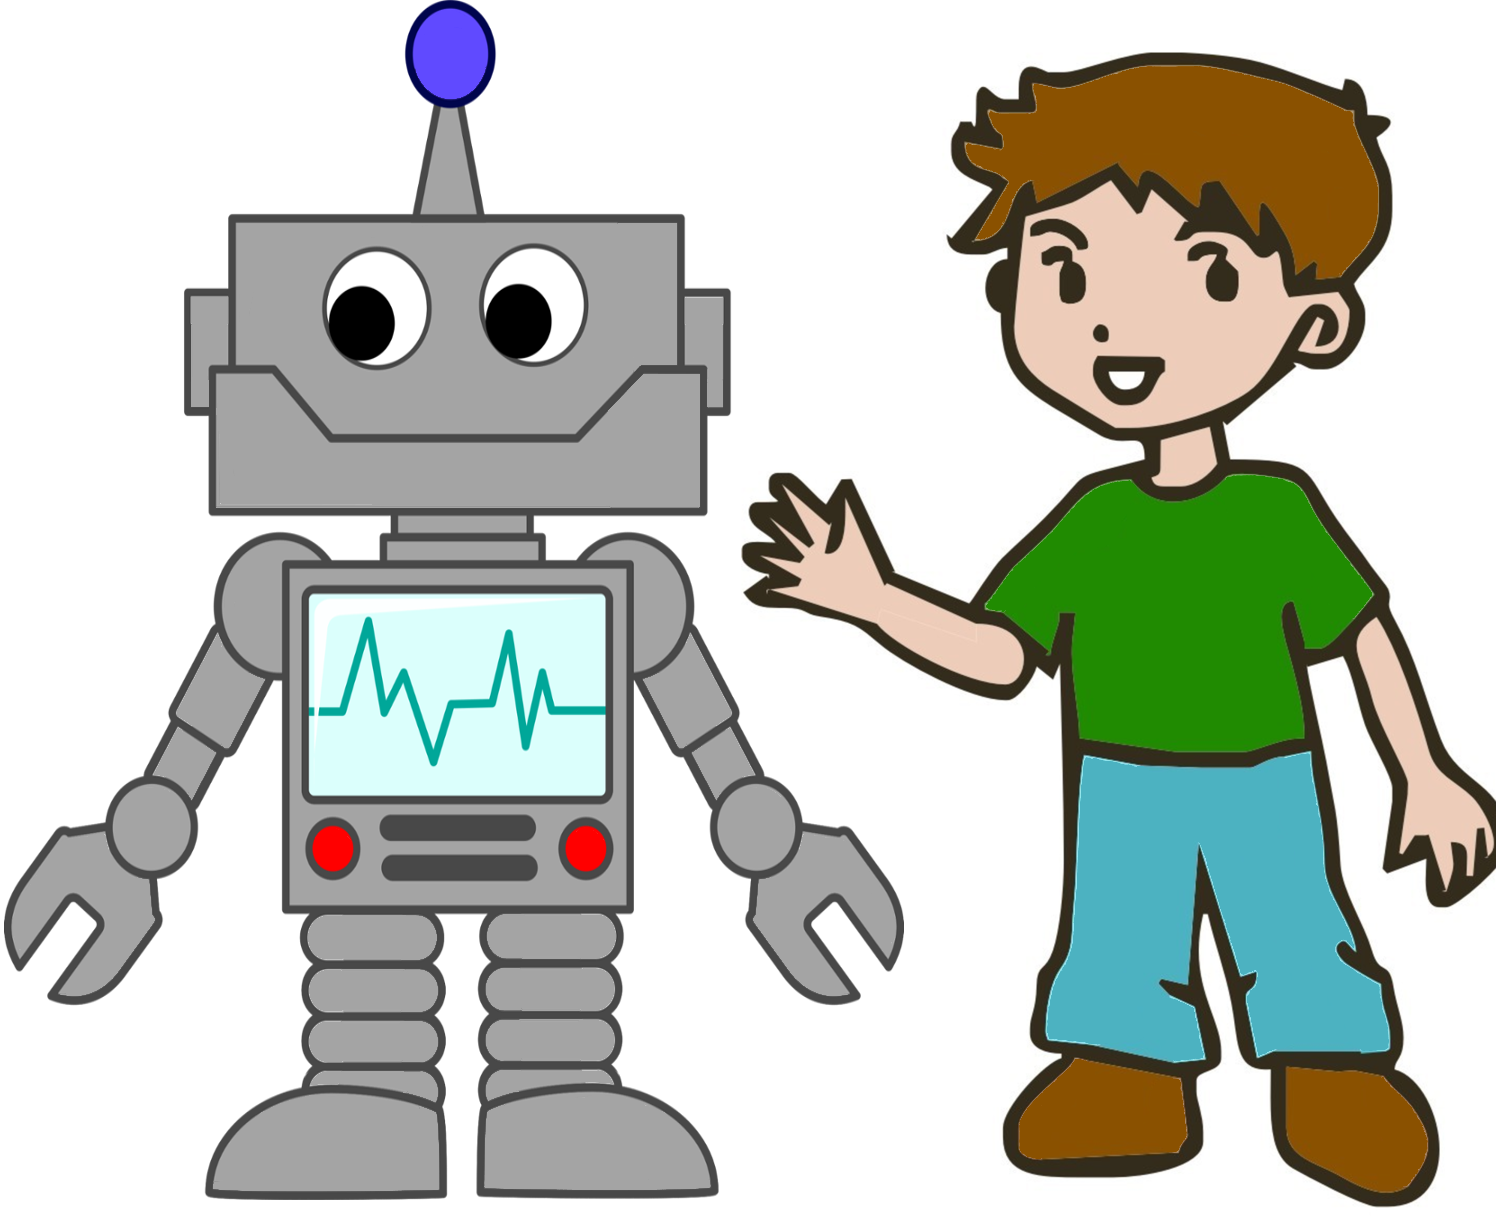
\includegraphics[width=0.5\columnwidth]{cover_pic}

\myVertSpace

\large

\textbf{\myThesisTitle}

\vspace{0.75cm}

\myFullName

\myVertSpace
\endgroup

\large

\textbf{Supervisor}: Doctor Alexandre José Malheiro Bernardino

\textbf{Co-Supervisor}: Doctor Giampiero Salvi

\textbf{Co-Supervisor}: Doctor Lorenzo Jamone

\myVertSpace

\centering

Thesis approved in public session to obtain the PhD Degree in\\Electrical and Computer Engineering

\vspace{0.75cm}

Jury final classification: Pass with Distinction

\vspace{\fill}

\textbf{2019}
\end{titlepage}

\restoregeometry

%!TEX encoding = UTF-8

\newgeometry{
    left=3cm,right=3cm,
    top=1cm,bottom=3cm
}

\begin{titlepage}
\setlength{\parindent}{0pt}

\includegraphics[bb=9.5cm 11cm 0cm 0cm,scale=0.23]{IST_A_CMYK_POS}

\begingroup
\centering

\vspace{0.75cm}

\Large
\textbf{UNIVERSIDADE DE LISBOA\\
INSTITUTO SUPERIOR TÉCNICO}

\myVertSpace

\large

\textbf{\myThesisTitle}

\vspace{0.75cm}

\myFullName

\myVertSpace
\endgroup

\large

\textbf{Supervisor}: Doctor Alexandre José Malheiro Bernardino

\textbf{Co-Supervisor}: Doctor Giampiero Salvi

\textbf{Co-Supervisor}: Doctor Lorenzo Jamone

\myVertSpace

\begingroup
\centering

Thesis approved in public session to obtain the PhD Degree in\\Electrical and Computer Engineering

\vspace{0.75cm}

Jury final classification: Pass with Distinction

\myVertSpace

\textbf{Jury}

\endgroup

\textbf{Chairperson}: Doctor João Manuel Lage de Miranda Lemos, Instituto Superior Técnico, Universidade de Lisboa

\textbf{Members of the Committee}:\\
Doctor José Alberto Rosado dos Santos Vítor, Instituto Superior Técnico,\\ Universidade de Lisboa

Doctor Ana Maria Severino de Almeida e Paiva, Instituto Superior Técnico,\\ Universidade de Lisboa

Doctor Luís Filipe de Seabra Lopes, Universidade de Aveiro

Doctor Alexandre José Malheiro Bernardino, Instituto Superior Técnico,\\ Universidade de Lisboa

Doctor Emre Uğur, Engineering Faculty, Boğaziçi University, Turkey

\vspace{0.75cm}

\textbf{Funding Institutions}:\\
Fundação para a Ciência e a Tecnologia

European Commission

\vspace{\fill}

\centering
\textbf{2019}
\end{titlepage}

\restoregeometry


% abstracts
%!TEX encoding = UTF-8

\chapter{Abstract}

%!TEX encoding = UTF-8

Personal and service robots may benefit society in different activities and challenges, thanks to their increasingly advanced mechanical and decision-making capabilities.
However, for that to happen one of the essential conditions is to have coherent, natural and intuitive interfaces so that humans can make a fruitful and effective use of these intelligent machines.
In general, the goal of reaching intuitive interfaces for \hri{} has not yet been attained, partly due to the fact that robots are not yet widespread in public spaces, partly due to the technical difficulties in interpreting human intentions.

Making service robots that understand their surroundings entails that they should possess capabilities that allow them to operate in unstructured environments and under unpredictable conditions, unlike industrial robots which usually operate in highly structured, controlled and repeatable environments.
To tackle these challenges, in this thesis we develop computational models based on findings from developmental psychology~(object affordances) and from neuroscience~(mirror neuron system).
The proposed models stem from the consideration that objects carry information about actions and interactions.

We contribute a modular framework for visual robot affordance learning, based on autonomous robot exploration of the world, sensorimotor data collection and statistical models.
We combine affordances with communication (gestures and language), to interpret and describe human actions in manipulative scenes by reusing previous robot experience.
We show a model that deals with multiple objects, giving rise to tool use, including the link from hand affordances~(i.e., action possibilities by using the hands) to tool affordances~(i.e., action possibilities by using tools).
We illustrate how affordances can be used for planning complex manipulation tasks under noise and uncertainty.
In two appendixes,
we describe a robot model for recognizing human gestures in manipulation scenarios,
and we report a study about how people perceive robot gestures when the facial information is turned off.

\bigskip

\textbf{Keywords}: \myThesisKeywords


%!TEX encoding = UTF-8

\chapter{Resumo}

%!TEX encoding = UTF-8

\begin{otherlanguage*}{portuguese}
Os robôs pessoais e de serviço podem beneficiar a sociedade em atividades e desafios diferentes, graças às suas capacidades mecânicas e de tomadas de decisão cada vez mais avançadas.
No entanto, para isso acontecer, uma das condições essenciais é a existência de interfaces coerentes, naturais e intuitivas para que os humanos possam usar estas máquinas inteligentes de uma forma frutuosa e eficaz.
No geral, o objetivo de alcançar interfaces intuitivas para a interação homem--robô (\emph{\hri}) não foi ainda alcançado, em parte pelo facto de que os robôs não estão ainda difusos nos espaços públicos, em parte devido às dificuldades técnicas na interpretação das intenções humanas.

Construir robôs de serviço, que percebam o que os rodeia, implica que os mesmos possuam capacidades que lhes permitam funcionar em ambientes não estruturados e em condições imprevisíveis, ao contrário dos robôs industriais que operam em ambientes altamente estruturados, controlados e repetíveis.
Para enfrentar estes desafios, nesta tese desenvolvemos modelos computacionais baseados em descobertas da psicologia do desenvolvimento~(potencialidades de objetos, \emph{object affordances}) e da neurociência~(sistema de neurónios espelho).
Os modelos propostos resultam da consideração que os objetos transportam informação sobre ações e interações.

Propomos uma biblioteca de \emph{software} modular para aprendizagem de potencialidades visuais em robôs, baseada na exploração autónoma do mundo, recolha de dados sensório-motores e técnicas estatísticas.
Juntamos potencialidades com comunicação (gestos e linguagem), para interpretar e descrever ações humanas em cenários de manipulação, reutilizando a experiência prévia do robô.
Mostramos um modelo que lida com objetos múltiplos, permitindo o uso de ferramentas, e também a ligação de potencialidades de mãos~(i.e., possibilidade de ações usando as mãos) para potencialidades de ferramentas~(i.e., possibilidade de ações usando ferramentas).
Explicamos como as potencialidades podem ser usadas para o planeamento de ações complexas de manipulação, sob ruído e incerteza.
Em dois apêndices,
descrevemos um modelo robótico para reconhecer gestos humanos em contextos de manipulação,
e relatamos um estudo de como as pessoas percebem gestos robóticos quando a informação facial dos mesmos é desligada.

\bigskip

\textbf{Palavras-chave}: \myPortugueseThesisKeywords
\end{otherlanguage*}



% acknowledgements
%!TEX encoding = UTF-8

\chapter{Acknowledgments}

First of all, I would like to give a warm thank you to my main supervisor, Prof.~Alexandre~Bernardino, for his constant guidance during the years that led to the preparation of this work, and for encouraging me to gain my independence. My co-supervisors, Prof.~Giampiero~Salvi and Prof.~Lorenzo~Jamone, have also supported me countless times with scientific insights, challenges, and suggestions, for which I am grateful.

I extend my gratitude to Prof.~José~Santos-Victor, director of the Computer and Robot Vision Laboratory~(VisLab) in Lisbon, for making me feel welcome, for making me feel an important ``player'' in a research team, and for creating an environment where it is possible to conduct research without worries. Thank you to all my laboratory mates as well~(too many to list!).

This research has been made possible with funding from the Portuguese Government (Fundação para a Ciência e a Tecnologia, doctoral grant SFRH/BD/61910/2009, project grants PEst-OE/EEI/LA0009/\allowbreak2011 and UID/EEA/50009/2013) and from the European Commission (POETICON++ project, FP7-ICT-288382).

The picture on the thesis cover was elaborated by me, modifying two open-access clipart images available from~\url{https://openclipart.org}, respectively drawn by Sirrob01~(robot image) and by an anonymous user~(boy image).

\bigskip

And finally, a heartfelt thanks to Cláudia for her unconditional patience and support all along.


% table of contents and other lists
\tableofcontents

\cleardoublepage
\addcontentsline{toc}{chapter}{\tocEntry{List of Figures}}
\listoffigures

\cleardoublepage
\addcontentsline{toc}{chapter}{\tocEntry{List of Tables}}
\listoftables

% list of acronyms, abbreviations and notation
%!TEX encoding = UTF-8

% https://tex.stackexchange.com/a/193799
\addchap{List of Acronyms}

\begin{acronym}
\acro{AHA}{Augmented Human Assistance}

\acro{AI}{Artificial Intelligence}

\acro{ASR}{Automatic Speech Recognition}

\acro{AI}{Artificial Intelligence}

\acro{BDe}{Bayesian Dirichlet likelihood-equivalence}

\acro{BN}{Bayesian Network}

\acro{CFG}{Context-Free Grammar}

\acro{CPD}{Conditional Probability Distribution}

\acro{CRF}{Conditional Random Field}

\acro{DAG}{Directed Acyclic Graph}

\acro{DoF}{Degree of Freedom}
\acrodefplural{DoF}[DoF]{Degrees of Freedom}

\acro{DMP}{Dynamic Movement Primitive}

\acro{EM}{\EMlong}

\acro{GMM}{Gaussian Mixture Model}

\acro{GPGPU}{General-Purpose Computing on Graphics Processing Units}

\acro{GRT}{Gesture Recognition Toolkit}

\acro{GT}{Ground Truth}

\acro{HMM}{Hidden Markov Model}

\acro{HPN}{Hierarchy Planning in the Now}

\acro{ISO}{International Organization for Standardization}

\acro{LBP}{Local Binary Pattern}

\acro{LoC}{Lines of Code}

\acro{MAP}{Maximum A Posteriori}

\acro{MCMC}{Markov Chain Monte Carlo}

\acro{MRF}{Markov Random Field}

\acro{MTRNN}{Multiple Timescales Recurrent Neural Network}

\acro{NLU}{Natural Language Understanding}

\acro{OAC}{\ObjAct{} Complex}
\acrodefplural{OAC}{\ObjAct{} Complexes}

\acro{PCA}{Principal Component Analysis}

\acro{PDDL}{Planning Domain Definition Language}

\acro{PDF}{Probability Density Function}

\acro{RNN}{Recurrent Neural Network}

\acro{RGB-D}{Red, Green, Blue and Depth}

\acro{ROS}{Robot Operating System}

\acro{SIFT}{Scale-Invariant Feature Transform}

\acro{SVM}{Support Vector Machine}

\acro{SoC}{System on Chip}

\acro{YARP}{Yet Another Robot Platform}
\end{acronym}


%%%%%%%%%%%%%%%%%%%%%%%%%%%%%%%%%%%%%%%%%%%%%%%%%%%%%%%%%%%%%%%%%%%%%%%%%%%%%%%%
\mainmatter
%%%%%%%%%%%%%%%%%%%%%%%%%%%%%%%%%%%%%%%%%%%%%%%%%%%%%%%%%%%%%%%%%%%%%%%%%%%%%%%%

% underline my name when listing publications with \fullcite
\underlinename{Saponaro}{Giovanni}{G.}

%!TEX encoding = UTF-8

\chapter{Motivation and Scope of the Thesis}
\label{chap:motivation}

In recent years, it is becoming increasingly common to use robots in domestic and public spaces. The total number of professional service robots sold in~2016~(i.e., non-industrial robots) rose considerably by~24\% to~\num{59706} units, up from~\num{48018} in~2015, with similarly positive forecasts expected for the period until~2020\footnote{Executive Summary World Robotics~2017 Service Robots, \url{http://www.ifr.org/service-robots/statistics/}}.
When deployed in domestic and public environments, robotic machines are expected to take on roles such as personal home assistants, receptionists, waiters, couriers, and more.
It is now feasible, though not without problems, to think of social robots being located in the same physical areas as a person.
This societal shift bears the issue of how to make robots that work effectively alongside humans.
In other words, how to build robots that possess the capabilities~(e.g., perception, reasoning, action) to execute their tasks well, and that in doing that are robust and reactive to uncertainty~(e.g., noisy measurements) and unexpected events~(e.g., failures), and that collaborate with us adequately by assisting our activities, without being a costly encumbrance in terms of money, time, or patience.
Public scenarios require interfaces that are easy to use for the general public, including for special groups like disabled, elderly or technology challenged people.
Human users should be able to provide instructions to robots in a natural and effortless way, mainly with verbal language and with nonverbal communication~(e.g., with body gestures), but this task has not been attained in general.
This thesis contributes to bridging the usability gap that human users face when dealing with robots.

One of the open challenges in designing robots that operate successfully in the \emph{unpredictable} human environment is how to make them able to foresee what actions they can perform onto objects of the world, and what the effects of these actions will be: in other words, how to provide them with the ability to perceive object \emph{affordances}~(action possibilities), a concept originally introduced in the field of developmental psychology in the 1960s, and of increasing importance in robotic research~(see Fig.~\ref{fig:num_papers:aff}). \label{aff_definition}
First proposed by J.~Gibson~\cite{jgibson:2014}, an affordance is defined as: ``a resource that the environment offers any animal that has the capabilities to perceive and use it''.
Later, E.~Gibson studied the role of affordances and learning in children~\cite{egibson:2003:ep}, reflecting on ``discovering the information that specifies an affordance''.
These theories stress how \emph{interacting} with the environment~(i.e., acting on it with a body) and \emph{perceiving} the environment~(i.e., sensing relevant features and changes of the world) are interconnected and related.

Suppose that a robotic agent has to operate in an environment, in particular having to see and use the objects that are available in order to achieve a given goal, such as adding sugar to a coffee~(\emph{stirring the coffee}) in the presence of a cup with coffee, of a sugar bowl, and of a spoon~(ignoring, for simplicity, the aspect of how the goal was entered into the system by a human user).
Classical \ac{AI} and robotic systems~\cite{russell_norvig:ai3,siciliano:2016:handbook2} will permit the agent to achieve the goal, relying on perceptual sensing algorithms, symbolic planning, and robot manipulator control, \emph{provided that the objects are recognized correctly}, meaning that the ``ingredients'' needed for the task~(e.g., cup, bowl, spoon) have been previously learned by the system at training time, and are detected at testing time.
However, what happens when a spoon is not available, or its appearance and shape are considerably different from the spoons that the system was taught?
Classical \ac{AI} may not be able to cope with this scenario, whereas the incorporation of affordances can help filling in the gaps in the following sense.
Reasoning on the affordances of the objects gives the benefit of relying on the knowledge about an object's \emph{functional features} or sub-parts, rather than on knowing the object's name or identity.
In the coffee example, if no spoon is available, the agent could use another type of cutlery which is long and thin, but if even that is not available, it might use yet another object that would help stir the coffee~(e.g., an object with a thin and elongated shape, as in the upper part of Fig.~\ref{fig:two-streams_cv}).
Affordances are mental shortcuts for accessing properties of objects that lead to a goal-directed action, without having to explicitly recognize the object name or type.
Therefore, affordances are a means to \emph{generalization} in robotic perception.
\label{coffee_example}

A similar argumentation can be made when we consider instructions provided by a human user to another agent~(human or robot).
In interactions, too, \emph{objects carry key information} about the action, which is conveyed explicitly or implicitly.
Humans can instruct other agents to perform operations on objects by saying their explicit name out loud~(using a shared verbal language which is understood by partners), or by referring to their distinctive features in an ambiguous situation~(e.g., by saying ``the large green box''), or by pointing at the objects themselves~(using a shared nonverbal gesture while communicating with an interaction partner).
Interestingly, when a person makes a gesture that points in the direction of an object, a system can reason on the affordances of the pointed object, which is useful for \emph{action prediction}~(i.e., predicting what the person will do next, or intends to do).
Indeed, when a person refers~(in whichever way) to an object, they are often really referring to the useful properties of it.
All in all, we can summarize these examples by saying that an object can act as a \emph{mediator for interaction}.
\nopagebreak[1]
Affordances are one way to exploit this power.
\label{action_prediction}

\begin{figure}[t!] % force footnote to appear on same page
\centering
\subfloat[][Number of published papers including ``affordances'' and ``robots'' in their text.]
{ 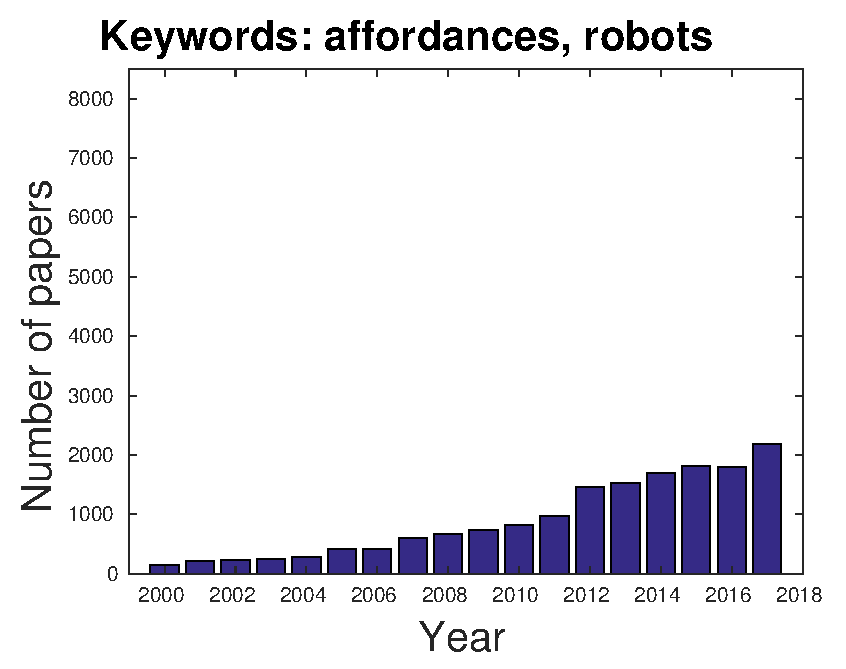
\includegraphics[width=0.45\textwidth]{num_papers_aff} \label{fig:num_papers:aff} } \quad
%
\subfloat[][Number of published papers including ``gestures'' and ``robots'' in their text.]
{ 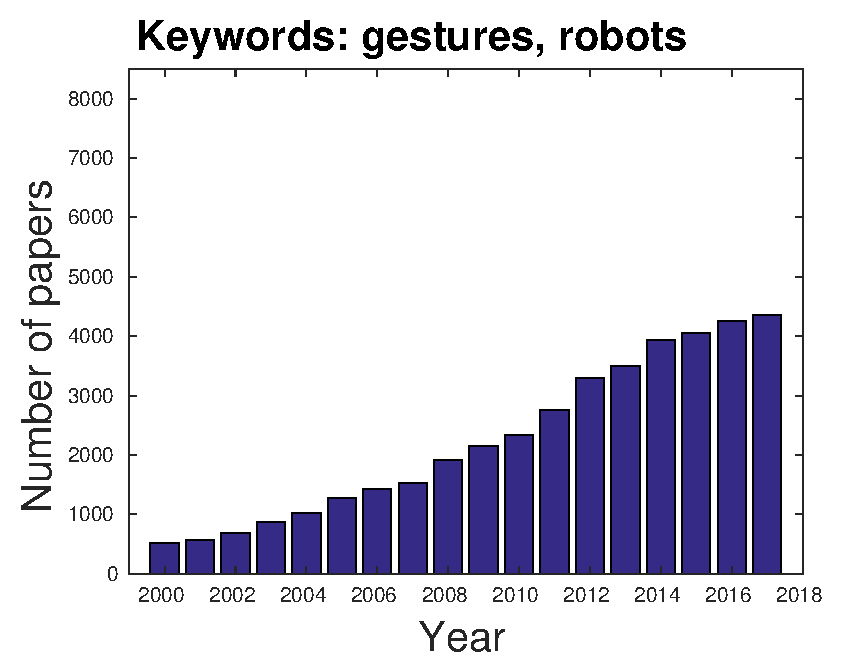
\includegraphics[width=0.45\textwidth]{num_papers_gest} \label{fig:num_papers:gest} } \\
%
\subfloat[][Number of published papers including the sentence ``\hri'' in their text.]
{ 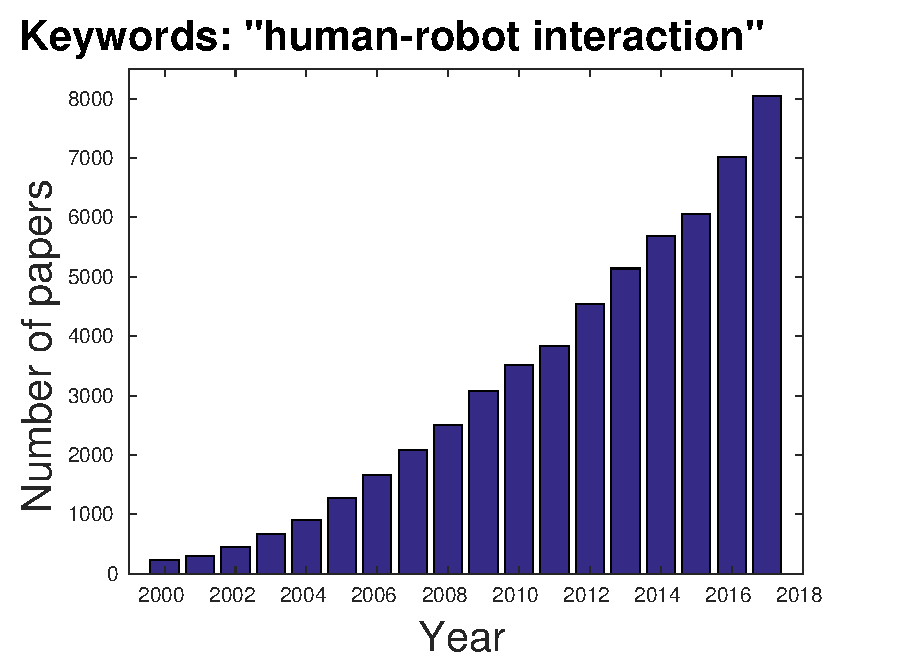
\includegraphics[width=0.45\textwidth]{num_papers_hri_in_quotes} \label{fig:num_papers:hri_in_quotes} } \quad
%
\subfloat[][Number of published papers including all of the keywords ``affordances'', ``gestures'', ``\hri'' and ``robots'' in their text.]
{ 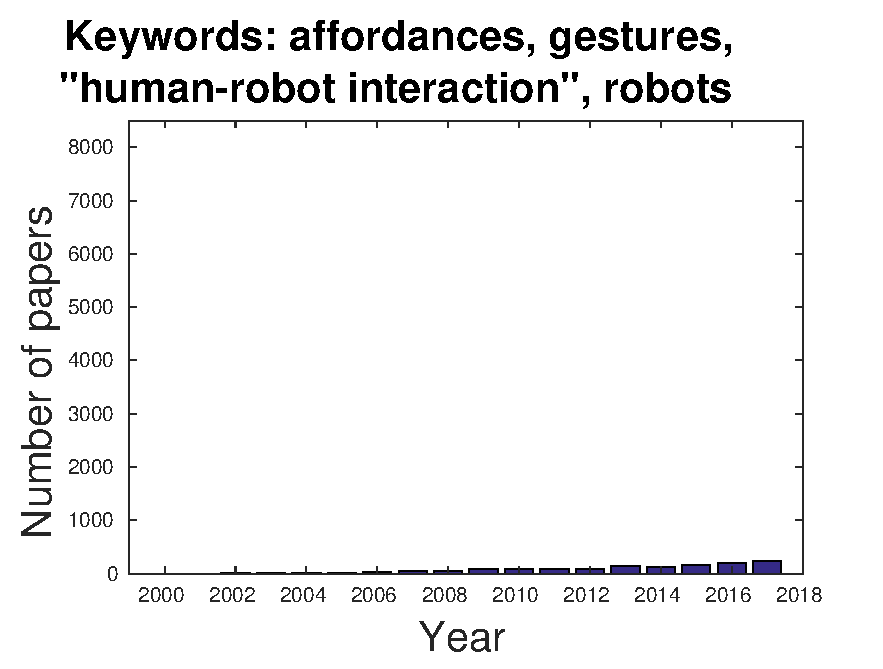
\includegraphics[width=0.45\textwidth]{num_papers_all} \label{fig:num_papers:all} }
% \cprotect protects \verb
% footnote within caption, https://tex.stackexchange.com/a/67030
\cprotect\caption[Number of published papers including relevant thesis keywords over time.]{Number of published papers including relevant thesis keywords over time. The searches in Fig.~\ref{fig:num_papers:aff}--\ref{fig:num_papers:hri_in_quotes} show a growing trend in terms of number of publications for individual topics, however Fig.~\ref{fig:num_papers:all} reveals that not many papers address all the considered topics jointly.
Plots computed from Google Scholar data, using the \verb!academic-keyword-occurrence! script by Volker Strobel\protect\footnotemark.}
\label{fig:num_papers}
\end{figure}
\footnotetext{\url{http://doi.org/10.5281/zenodo.1218409}}

Within robotic research, in addition to a growing interest in affordances as mentioned above, there has been a similar trend in topics such as body gestures~(see Fig.~\ref{fig:num_papers:gest}) and, in general, in \hri{} systems and studies~(see Fig.~\ref{fig:num_papers:hri_in_quotes}).
However, there are not many papers yet that address these topics \emph{jointly}, as seen in Fig.~\ref{fig:num_papers:all}: the number of published papers which mention all of the keywords~(in the entirety of the article text, not only in the title) ranges between~3 in year~2000 and about~180 in~2016.
Even though~180 papers is a reasonable number, it still constitutes a relatively small fraction of the whole body of articles produced by the robotics community yearly.

\section{Objectives}

This thesis revolves around the usefulness of affordances in robots, and the possible \emph{advantages of using robot affordances in conjunction with other modalities, such as human body gestures and language, for supporting effective interactions between humans and robots}.
The core goal is to develop computational models to use affordances and other environment elements in order to close the gap between human and robot knowledge.
We research how object affordances can provide a \emph{joint reference} between human and robot for the correct interpretation of gestural instructions, and how this can ultimately lead to intuitive robot utilization for the general population.
In particular, this work stems from the observation that objects contain important links to physical actions and action understanding when interacting with other agents.
From this idea, we develop a theory comprising objects affordances, body gestures and probabilistic inference.
We contribute software programs that can be deployed on real robotic systems.
We show a number of practical contributions in robot algorithms that incorporate the above concepts.

By advancing action recognition capabilities in robots through the combination of gestures and affordance perception, we also \allowbreak endow \allowbreak robots with the ability to recognize human actions during their enactment, i.e., before said actions are completed in their entirety.
The advantage is to provide robots the ability to \emph{anticipate} human actions and intentions, given contextual circumstances.
We show this anticipatory behavior and capability in \hr{} collaborative tasks, relying on the information provided by objects affordances, body gestures and probabilistic inference.

\begin{figure}
    \newcommand{\myscaleaffmodels}{0.45}
    \centering
    \subfloat[][Computational model of robot affordances by Montesano~\cite{montesano:2008}, explained in Ch.~\ref{chap:background}.]
    { \begin{tikzpicture}[scale=\myscaleaffmodels, every node/.style={transform shape}]
      \montesanoAE
      \montesanoO
      \end{tikzpicture} \label{fig:aff_models_intro:montesano}
    } \quad
    %
    \subfloat[][Computational model of affordances with associated verbal descriptions, by Salvi~\cite{salvi:2012:smcb}, explained in Ch.~\ref{chap:background}.]
    { \begin{tikzpicture}[scale=\myscaleaffmodels, every node/.style={transform shape}]
      \montesanoAE
      \montesanoO
      \salviW
      \end{tikzpicture} \label{fig:aff_models_intro:salvi}
    } \\
    %
    \hspace{-9cm} \footnotesize \emph{state of the art} \\
    \hrule
    \hspace{-9cm} \emph{our contributions} \normalsize \\
    %
    \subfloat[][Computational model of affordances with gestures and language, proposed in Ch.~\ref{chap:gestures}.]
    { \begin{tikzpicture}[scale=\myscaleaffmodels, every node/.style={transform shape}]
      \montesanoAE
      \montesanoO
      \saponaroGestRecBox
      \salviW
      \end{tikzpicture} \label{fig:aff_models_intro:gestures_lang}
    } \quad
    %
    \subfloat[][Computational model of affordances for dealing with multiple objects and tool use, proposed in Ch.~\ref{chap:tool}.]
    { \begin{tikzpicture}[scale=\myscaleaffmodels, every node/.style={transform shape}]
      \montesanoAE
      \saponaroManipulatorUseBox
      \end{tikzpicture} \label{fig:aff_models_intro:tools}
    }
\caption[Schematic diagrams of the cognitive robotic \allowbreak models discussed in this thesis.]{Schematic diagrams of the cognitive robotic models discussed in this thesis.
They all include a representation of affordances as relations between actions, objects and effects (Figs.~\ref{fig:aff_models_intro:montesano}--\ref{fig:aff_models_intro:tools}).
In addition, some of them include extensions or specific aspects being highlighted (Figs.~\ref{fig:aff_models_intro:gestures_lang}--\ref{fig:aff_models_intro:tools}).
Figs.~\ref{fig:aff_models_intro:montesano} and~\ref{fig:aff_models_intro:salvi} are prior existing works from the state of the art, whereas Figs.~\ref{fig:aff_models_intro:gestures_lang} and~\ref{fig:aff_models_intro:tools} are contributions of this thesis.}
\label{fig:aff_models_intro}
\end{figure}

Fig.~\ref{fig:aff_models_intro} illustrates the cognitive robotic models used in this thesis schematically.
Fig.~\ref{fig:aff_models_intro:montesano} exemplifies the state of the art in robot affordances: a computational implementation of simple object affordances, defined as the relations between actions, objects and effects, as proposed in the works of Montesano~\cite{montesano:2008}.
Fig.~\ref{fig:aff_models_intro:salvi} is also prior work from the state of the art, focusing on the joint learning of affordances and language descriptions.
Fig.~\ref{fig:aff_models_intro:gestures_lang} shows our contribution of incorporating gestures and language descriptions to the model, allowing a cognitive robot to reason about physical actions when external agents operate in an environment shared with the robot, to describe the scene verbally, and permitting anticipatory behavior.
Fig.~\ref{fig:aff_models_intro:tools} depicts our contribution related to tool use, which allow a robot to not only use a single object of the world, but to reason about the possibilities offered by a first grasped object (i.e., using a specific manipulator) onto a second object which is acted upon when the first one is in the agent's hand.

\bigskip

In the following sections, we present the constituent theoretical components upon which this thesis is based.
Sec.~\ref{sec:motivation:devrob} defines the principles that guide the framework of developmental robotics,
Sec.~\ref{sec:motivation:affordances} illustrates the concept of affordances and the advantages that it provides in robotics, and
Sec.~\ref{sec:motivation:neuro} specifies the neuroscience theories which are linked to our research.
Finally, Sec.~\ref{sec:motivation:main_contributions} lists the main contributions of the thesis, and Sec.~\ref{sec:motivation:outline} gives a brief outline of the structure of the next chapters.

\section{Developmental Robotics}
\label{sec:motivation:devrob}

Developmental robotics, also known as epigenetic robotics or ontogenetic robotics, is a subfield of robotics whose main aims are (i)~modeling the development of \emph{increasingly complex cognitive processes}~(for example, the understanding of language, or the acquisition of manipulation skills), and also (ii)~understanding how such processes emerge through physical and social interaction~\cite{lungarella:2003:devrobsurvey,cangelosi:2015:devrobbook}.
Developmental robotics takes direct inspiration from the progressive learning phenomena observed in children's cognitive development.
It is related to other fields such as \ac{AI}, developmental psychology, neuroscience and dynamical systems theory.

In this line of research, robots are used to verify theoretical models of emergence and development of action and cognition.
The rationale is the following: if a model is instantiated inside a system embedded in the real world, many things can be learned about its strengths and limitations.
Developmental robotics operates on short~(ontogenetic) time scales of single individuals, or small groups of individuals.
By contrast, evolutionary robotics typically operates on long~(phylogenetic) time scales and large populations of several individuals.

The basic idea behind developmental robotics~(i.e., that the mechanism of development can be used to understand and to construct cognition) can be traced back to Turing~\cite{turing:1950}:
``Instead of trying to produce a programme to simulate the adult mind, why not rather try to produce one which simulates the child's? If this were then subjected to an appropriate course of education, one would obtain the adult brain''.
Another core idea in developmental robotics is \emph{embodiment}~(or Embodied \acl{AI}), which states that intelligence~(e.g., common sense) can only be the result of learned experience of a body living in the real world~\cite{pfeifer:2006}.

This thesis follows the developmental robotics perspective: the contributions that we will describe in the next chapters hinge on the paradigm of a robot that learns about its surrounding environment by incremental \emph{self-exploration}, starting from a limited initial knowledge; in addition, this learning process is embodied, in the sense that it is conditioned on a particular, physical robot body~(e.g., the arms and hands can reach and manipulate certain objects and locations in the robot workspace, but not all of them).

\section{Motivation for Using Robot Affordances}
\label{sec:motivation:affordances}

Affordances, introduced in p.~\pageref{aff_definition}, correspond to action possibilities offered to agents by elements of the environment.
They can support service robotics\footnote{The \ac{ISO} defines a ``service robot'' as a robot ``that performs useful tasks for humans or equipment excluding industrial automation applications'' (ISO~8373).} and \hri{} applications for a number of reasons.

\begin{figure}
\centering
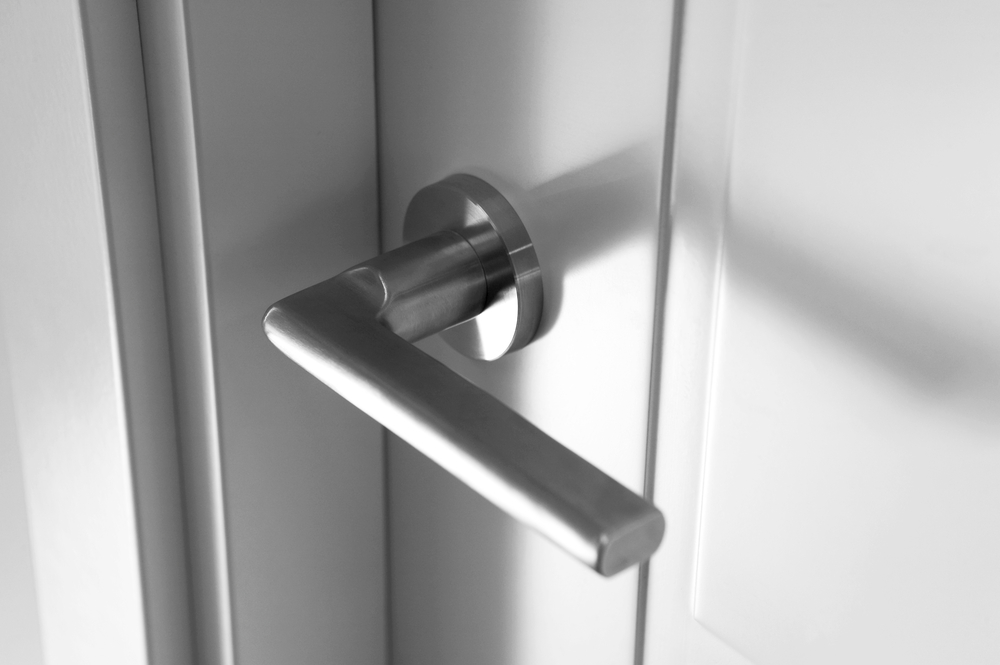
\includegraphics[width=0.9\textwidth]{door_handle.jpg}
\caption{A door handle affords the ability to be turned and pulled, resulting in the door to be open.}
\label{fig:door_handle}
\end{figure}

First, affordances are \emph{personal}: they depend on the agent~(or on the ``animal'', as in the original definition by J.~Gibson~\cite{jgibson:2014}).
For example, the door handle of Fig.~\ref{fig:door_handle} offers the affordance of being manipulated in order to open the door, but the precise motor realization of the act of turning the handle is different for an adult human or for a robot~(and also for other types of agents such as children or animals)~\cite{chemero:2003:outline,chemero:2007:gibsonian,jamone:2016:tcds}.
We can say that there is one set of affordances for humans and another one for robots.
Then, if a robot can understand both types, it can link human actions and robot actions.

Second, affordances are suited for learning and generalization behaviors on cognitive robots that manipulate objects of the world.
Modeling all the possible world interactions is unfeasible~(we cannot pre-program all the interactions between a robot, its motor action repertoire, and the resulting effects onto the objects of the world), therefore learning from experience is required.
However, to collect large amounts of robot sensorimotor data is challenging and costly.
Robot affordances are then one possibility to capture meaningful aspects of data, without necessarily requiring large amounts of data, but permitting to learn a model that can adapt to situations unseen during training.
We describe this aspect in Ch.~\ref{chap:background}.

Third, affordances can be profitably combined with \emph{communication}, both verbal~(i.e., language) and nonverbal~(i.e., gestures).
For example, the ability to foresee the action performed by other human agents onto physical objects is fundamental for successful \emph{anticipation} and collaboration in joint tasks.
If a robot can perceive the affordances offered to a human by objects present in a collaborative \hr{} scenario, it can monitor the evolution of the task, anticipate the final goal, and intervene in a timely manner.
We explore this aspect in Ch.~\ref{chap:gestures}.

Fourth, learning how humans operate \emph{tools} is crucial for having a robot operate in complex manipulation tasks that are typical in human-like environments.
We note that \emph{our hands are our first tools} in interacting with physical objects of the world; then, from~16~months of age, humans start developing functional tool use~\cite{fagard:2014:emergence}.
We investigate this transition on a humanoid robot, modeling the transfer from hand affordances~(i.e., perception of action possibilities offered by objects using different hand morphologies) to tool affordances~(i.e., perception of action possibilities offered by objects using different tools).
A robot can learn tool use capabilities in a gradual way, generalizing to different tools that afford different possibilities, similarly to how children progressively learn mutual interactions between different objects. Acquiring this capability permits a robot to perform actions that would otherwise not be possible, for example grasping a faraway object with the help of an elongated tool.
We explore these aspects in Ch.~\ref{chap:tool}.

Fifth, robot sensorimotor knowledge~(in the form of learned affordances) can be useful for symbolic reasoning in order to form a unified \emph{planning architecture} that allows a robot to carry out a complex manipulation task under challenging conditions and external disturbances~(e.g., noisy perception, motor problems, obstruction by other agents).
We present a case study about the POETICON++ project, which tackled all of those issues, in Ch.~\ref{chap:poeticon++_case_study}, introducing a robust action planning system that combines robot sensorimotor knowledge~(in the form of learned affordances) with symbolic reasoning, using a unified probabilistic representation.

\section{Neuroscience Inspiration}
\label{sec:motivation:neuro}

In this work we draw inspiration from neuroscience~(the science that deals with the function and structure of the nervous system and brain), in particular from the following concepts:
two-streams hypothesis; \allowbreak
canonical neurons and mirror neurons.
We will now briefly explain these ideas.

\subsection{Two-Streams Hypothesis}
\label{sec:motivation:neuro:twostreams}

\begin{figure}
\centering
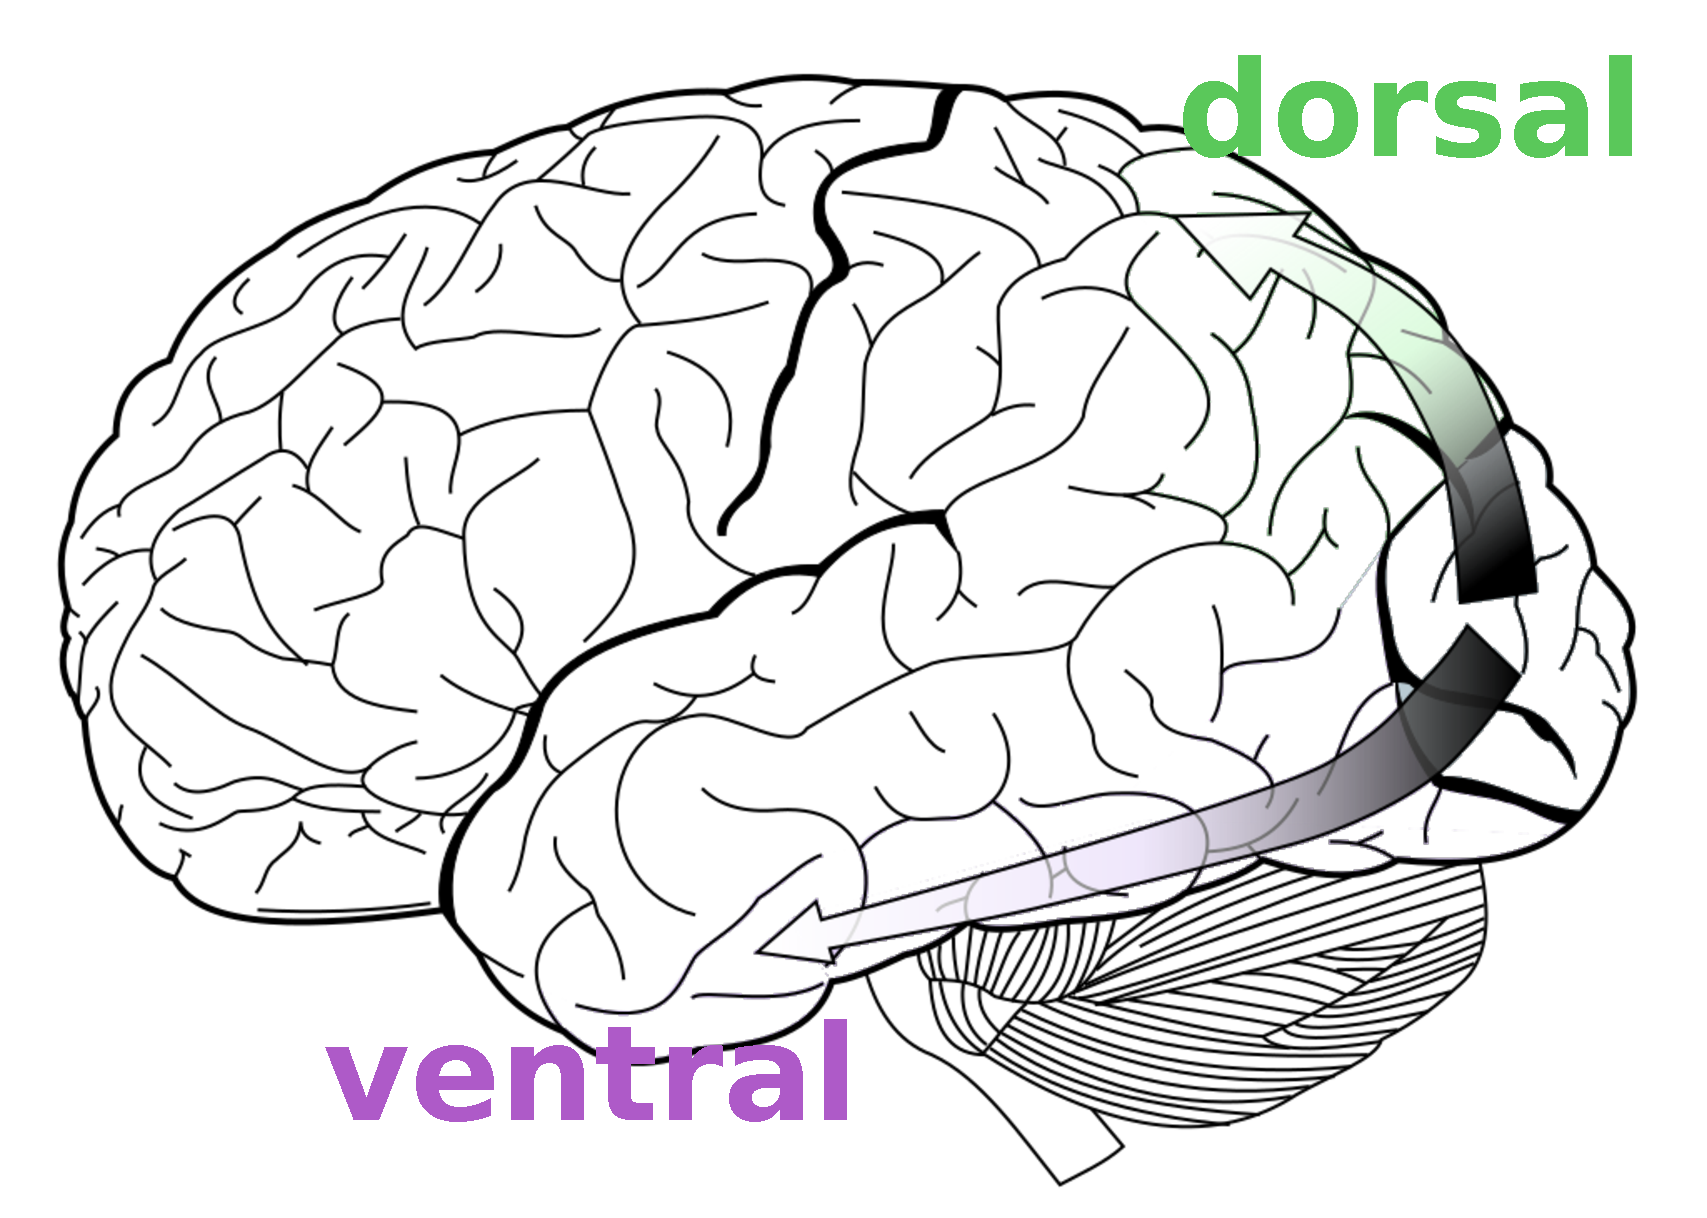
\includegraphics[width=0.9\textwidth]{two-streams_hypothesis_brain}
\caption[Graphical illustration of the visual processing streams in the human brain according to the two-streams hypothesis.]{Graphical illustration of the visual processing streams in the human brain according to the two-streams hypothesis.
The ventral stream~(lower part of figure) is shown in purple, stretching from the visual cortex into the temporal lobe.
The dorsal stream~(upper part) is shown in green, stretching from the visual cortex into the parietal lobe.
Picture elaborated under the CC BY-SA~3.0 license from an image by Wikimedia user Selket, author of the original picture at \url{https://commons.wikimedia.org/wiki/File:Ventral-dorsal_streams.svg}.}
\label{fig:two-streams_brain}
\end{figure}

The \emph{two-streams hypothesis}~\cite{goodale_milner:1992,chao:2000:neuro} speculates that the primate cerebral cortex processes visual information using two separate pathways:
\begin{enumerate}
\item the ventral or ``what'' stream, responsible for object categorization and recognition;

\item the dorsal or ``where'' or ``how'' stream, which guides object-directed actions such as reaching and grasping.
\end{enumerate}

\begin{table}
\caption[Main differences between the ventral stream and the dorsal stream.]{Main differences between the ventral stream and the dorsal stream, adapted and simplified from~\cite{norman:2002:bbs}.}
\label{tab:two-streams_differences}
\centering
\begin{tabular}{lll}
\toprule
factor & ventral stream & dorsal stream \\
\midrule
function        & object recognition & visually-guided behavior \\
                &                    & (e.g., reaching and grasping) \\
sensitivity     & details (high      & motion (high temporal \\
                & spatial frequency) & frequency) \\
memory          & long-term storage  & short-term storage \\
speed           & slow               & fast \\
consciousness   & high               & low \\
reference frame & object-centered    & viewer-centered \\
                & (allocentric)      & (egocentric) \\
visual input    & foveal             & across all retina \\
\bottomrule
\end{tabular}
\end{table}

Fig.~\ref{fig:two-streams_brain} shows a graphical representation of the two streams in the human brain, whereas Table~\ref{tab:two-streams_differences} lists the main differences between the two pathways for the purpose of this thesis.
In particular, looking at the \emph{speed} characteristic~(i.e., speed of firing after receiving a visual stimulus), it has been observed that the ventral stream is relatively slow~\cite[p.~84]{norman:2002:bbs}, whereas the dorsal stream is faster~\cite{proverbio:2011:neuro}.
The dorsal pathway constitutes a direct, fast neural link~(\textasciitilde250~ms) between vision and motor activation areas in the human brain, bypassing other regions while performing tasks like object reasoning or recognition~\cite{tunik:2007:neuroimage}.
For example, when humans observe a small cup of coffee, they perceive the shape, the handle, and the action possibilities provided by that object (i.e., its affordances) through the fast dorsal stream, whereas the precise object classification provided by the slower ventral pathway does not have the same usefulness, depending on the task.

\begin{figure}
\centering
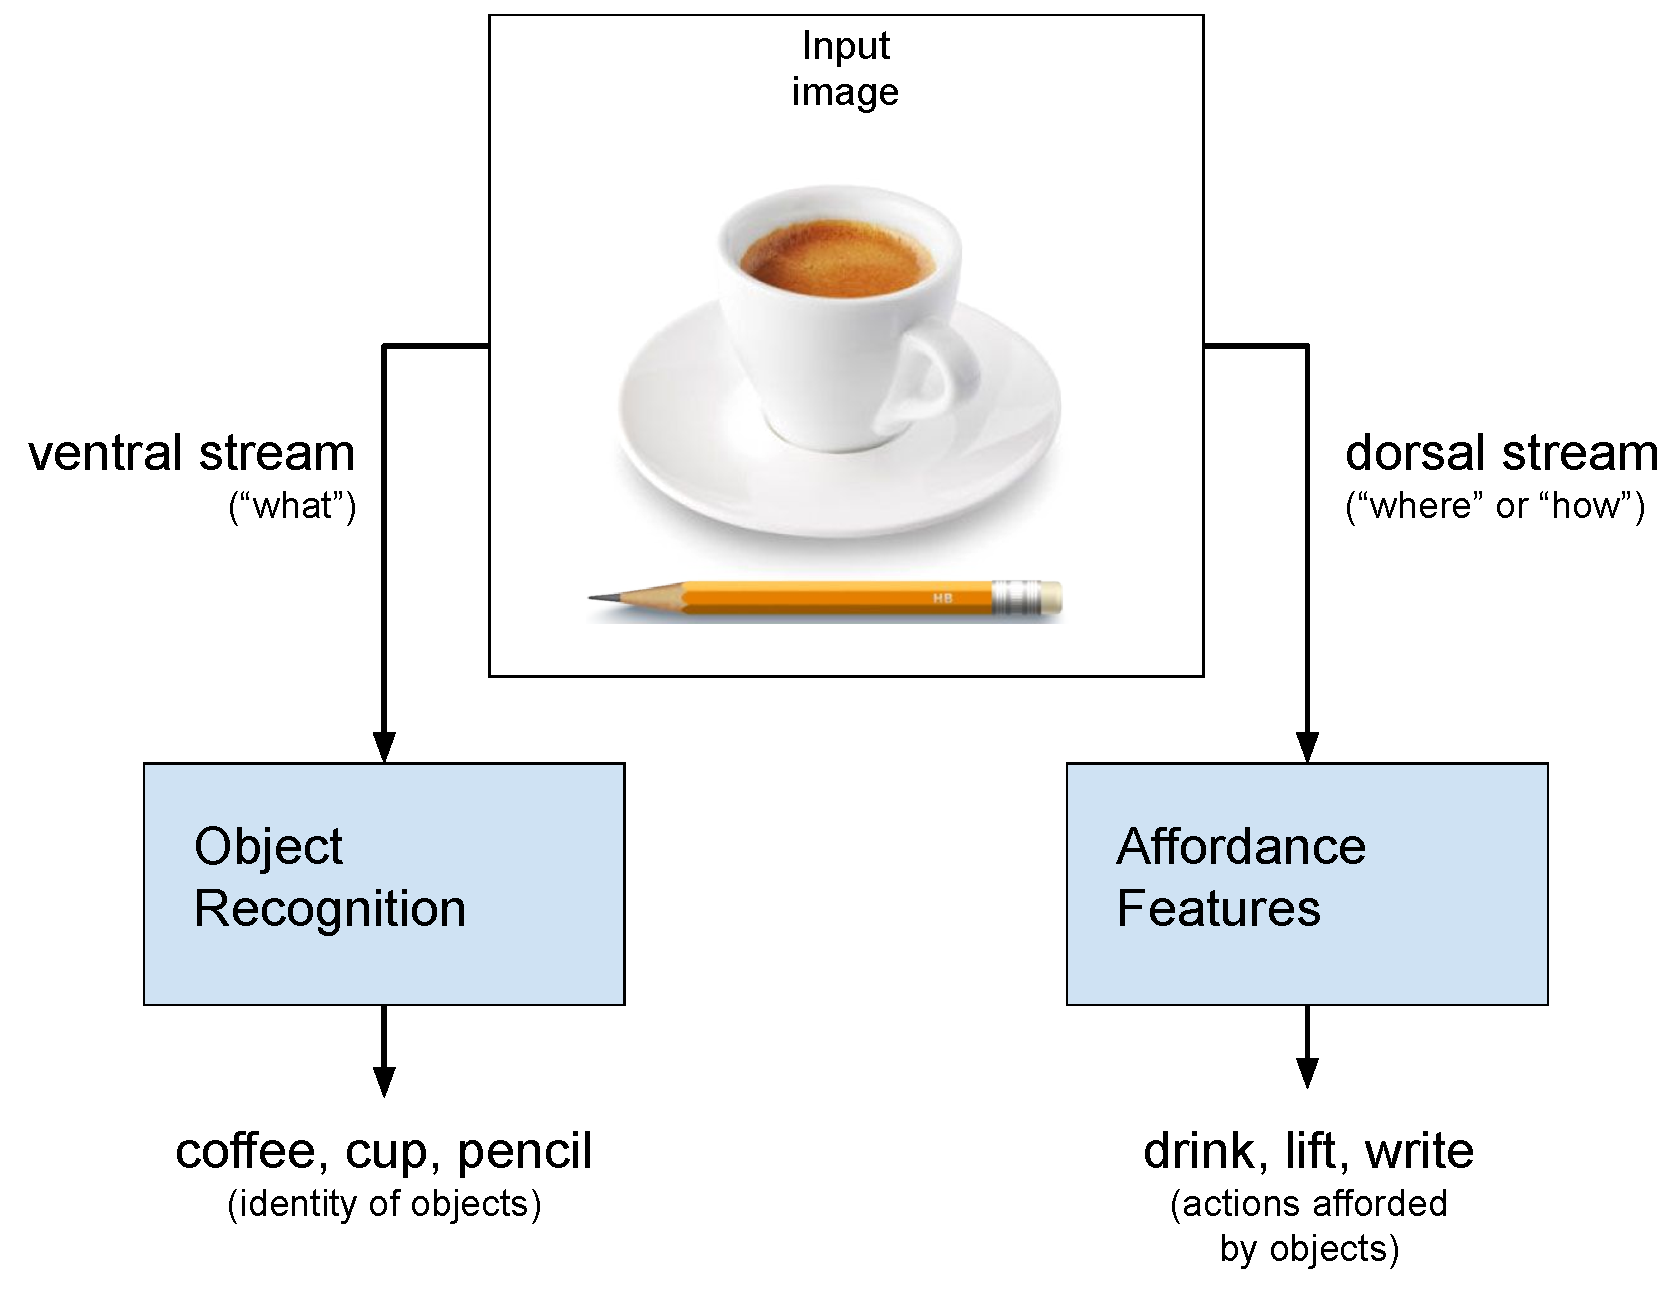
\includegraphics[width=0.9\textwidth]{two-streams_hypothesis_cv}
\caption[Illustration of the two-streams hypothesis from a computer vision point of view.]{Illustration of the two-streams hypothesis from a computer vision point of view.
The ventral and dorsal pathways are highlighted, having different features and scopes.
The work developed in this thesis mainly focuses on the dorsal pathway and on learning visual affordances, which does not require to know the identity of objects as in the ventral pathway.
However, in Ch.~\ref{chap:poeticon++_case_study}, we also show a case study that employs both types of object reasoning in parallel~(ventral and dorsal).}
\label{fig:two-streams_cv}
\end{figure}

The reason why this neuroscience theory can be fruitful for cognitive robotics is exemplified by looking at Fig.~\ref{fig:two-streams_cv}.
Each of the two streams has its own perceptual process~(with extracted features and outputs), depending on the intended application being considered.
In the case of the ventral stream, the application is typically object recognition: that is, identifying the label or name of objects present in the input image, provided that object classes have been previously learned by the system during a learning phase.

On the contrary, in the case of the dorsal stream, we seek visual object features that can be linked to functional properties of the object~(i.e., its affordances), without having to recognize the label of the object, that is, without having necessarily seen that object before.
Therefore, in the works reported in this thesis we rely on the dorsal stream type of reasoning, because it is a suitable model for \emph{reasoning on objects in a category-independent way}~(i.e., not focusing on the object name or category, but rather on its sub-parts and functional features).
To that end, we investigate the generalization capabilities provided by this type of reasoning~(e.g., when testing objects different from the ones seen during the training phase).
This dorsal pipeline is a complement to the ventral one, responsible for object recognition and categorization, which is a topic of its own in computer vision, outside the scope of this thesis.
However, in Ch.~\ref{chap:poeticon++_case_study}, we will show how it is possible and profitable to employ both types of object reasoning~(ventral and dorsal) in a scenario that involves \hri{} through spoken verbal requests by the human, action planning and manipulation by the robot.

All in all, we show how learned affordance skills can be leveraged by robots in several contexts and modalities: reasoning on tools, on hand postures, on human gestures, language, and for action planning during manipulation tasks.

\subsection{Canonical Neurons and Mirror Neurons}
\label{sec:motivation:neuro:canonical_and_mirror}

Certain classes of neurons have been observed to be active in primates~(apes and humans) not only during the execution of behaviors, but also during the perception of the objects that are related to these behaviors~\cite{rizzolatti:2004:arn}.

\emph{Canonical neurons} respond both during grasping action execution, and when we simply view an \emph{object of a particular shape}~\cite[Ch.~19]{kandel:2000:principles}.
In other words, these neurons have sensory properties such that they respond to the presentation of objects on which we can perform an action~(e.g., grasping).
The grasping of objects needs to be informed by the shape of the object: for instance, we grasp paperclips differently than how we grasp oranges.
The sensory input is used to drive appropriate grasping gestures.
Canonical neurons are not assumed to be responsible for visual recognition: they just receive relevant input from areas involved in the processing of visual features.
We use this idea to link geometrical features, computed from the shape of visually segmented objects, to robot affordances~(Ch.~\ref{chap:background}).

\emph{Mirror neurons} respond to the motor actions of others.
More precisely, according to the \emph{mirror neuron system} theory, there is a neurophysiological mechanism in the brain resulting in certain neurons firing in two different situations:
(i)~when performing a movement, or
(ii)~when sensing that a peer is performing a goal-directed movement~\cite{kilner:2009:jneurosci}.
The interpretation is that sensing and execution of movement are two sides of the same coin, and this mirroring mechanism is a fundamental part of action understanding and imitation learning skills~\cite{fogassi:2005:science,gazzola:2007:neuroimage}.
We use this idea to recognize manipulative gestures performed by external agents~(Ch.~\ref{chap:gestures})
and reasoning about the functional properties of the objects involved,
thus exploring action prediction and action anticipation capabilities~(as in the pointing gesture example of p.~\pageref{action_prediction})
integrating affordances with gestures.

People have an \apriori{} knowledge about others' body parts, and they use movement cues to understand what actions or gestures are being executed by others.
This mechanism can be replicated on a robot, encoding a gesture as the union of (i)~body part (appearance cue) and (ii)~movement.
We can interpret others' actions because what others do belongs to our motor repertoire or experience~\cite{rizzolatti:2001:nrn}.

\bigskip

To summarize, the contributions described in this thesis are based on a model of the environment surrounding the robot, with the novelty of representing the knowledge of this environment with affordances, beyond the mere recognition of specific objects.
Thus, our model looks at the physical objects present in the scene, their affordances, as well as people with their informative body gestures and actions.

\section{Contributions}
\label{sec:motivation:main_contributions}

The main contributions of this thesis are:
\begin{itemize}
\item a framework for visual robot affordance learning, based on autonomous robot exploration of the world, sensorimotor data collection and statistical models~(\aclp{BN}).
This system was implemented over the years 2010--2018 as a modular software to be deployed on humanoid robots, focusing on flexibility~(e.g., separating perception, learning and motor components, and allowing the user to employ some or all of them as needed) and real-time operations~(e.g., supporting robot cameras which capture images at~$30$ frames per second).
As a result, it was adopted as a building block for the further contributions of this thesis~(listed in the bullet points below), but it also had an impact externally, being adopted by other researchers: \cite{morse:2016:cogsci,dehban:2016:eccvws,dehban:2016:icra,dehban:2017:humanoids};

\item the combination of object affordances with communication (gestures and language).
This approach allows a robot to interpret and describe the actions of human agents by reusing the robot's previous experience.
This part produced the following publications:
\listPublicationsGestures

\item a model for tool use affordances in robots.
The main contributions were
(i)~the visual feature extraction component, capable of processing multiple objects simultaneously, extracting information both from the shape of whole objects as well as from their sub-parts;
(ii)~in the learning component, designing and evaluating various types of computational affordance models and parameters for assorted tasks (e.g., generalization to unseen objects; transfer of learned knowledge from a simulated robot to a real one);
(iii)~a method for learning the affordances of different robot hand postures, investigating the link from hand affordances~(i.e., action possibilities by using the hands) to tool affordances~(action possibilities by using tools).
This part produced the following publications:
\listPublicationsTools

\item a case study about the application of affordances and human verbal instructions for robot \emph{planning of manipulation tasks}, developed within the scope of the POETICON++ research project.
This part produced the following publications:
\listPublicationsPoeticonpp

\item an appendix that describes a novel human gesture recognition model for manipulative hand gestures, inspired by statistical techniques from \ac{ASR}.
It produced the following publication:
\listPublicationsAppendixGestureRecognition

\item finally, an appendix related to robot communication~(rather than robot perception and action, the core topics of the thesis):
the perceived social attitude attributed by non-technical users when observing certain head and body gestures performed by a robot.
This study paves the way for an active learning system capable of optimizing robot motion parameters with the aim of improving the communicative expressiveness.
It produced the following publication:
\listPublicationsAppendixHumanPercRobotGest

\end{itemize}

\section{Outline of the Thesis}
\label{sec:motivation:outline}

\begin{figure}
\centering
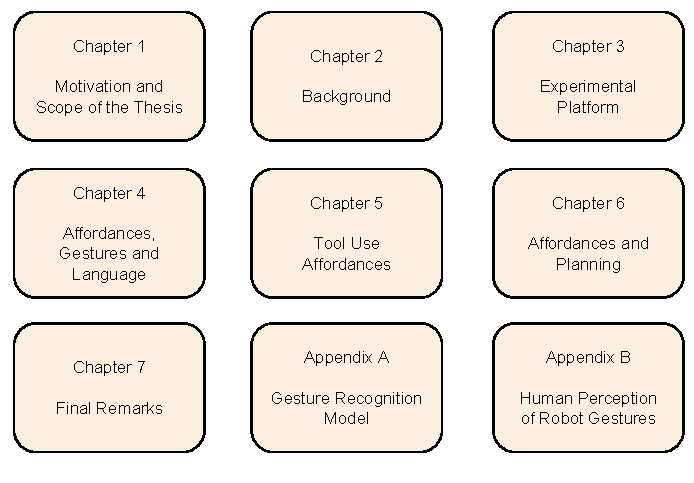
\includegraphics[width=0.9\textwidth]{chapters_diagram}
\caption{Structure of the thesis.}
\label{fig:chapters_diagram}
\end{figure}

The thesis is structured as sketched in Fig.~\ref{fig:chapters_diagram}.

Ch.~\ref{chap:background} illustrates
the main machine learning notation and concepts~(including \aclp{BN}) used in the thesis, and
the previous works in the literature which are related to our broad scope~(other chapters also contain specific related work sections).

Ch.~\ref{chap:platform} describes the experimental platform:
the iCub humanoid robot,
the experimental scenario under study, and
our modular software framework for robot affordance learning, focused on autonomous robot exploration of the world and visual processing, used as a building block in the rest of the thesis.

Ch.~\ref{chap:gestures} presents a computational model that combines affordances with language, broadly speaking.
It does that by incorporating
nonverbal language, in the form of \emph{human gestures}; and also
verbal language, by generating verbal descriptions of manipulative scenes.

Ch.~\ref{chap:tool} shows an affordance model that deals with multiple objects, giving rise to \emph{tool use}, including the link from hand affordances~(i.e., action possibilities by using the hands) to tool affordances~(action possibilities by using tools).

Ch.~\ref{chap:poeticon++_case_study} illustrates a case study about the application of affordances and human verbal instruction interpretation for robot \emph{planning of manipulation tasks}, developed within the scope of the POETICON++ research project.

Ch.~\ref{chap:final_remarks} draws the conclusions and lists the avenues for future work.

Appendix~\ref{chap:gesture_recognition} presents the details of the human gesture recognizer for manipulative hand gestures: this recognizer was inspired by statistical techniques from \ac{ASR}, and it was employed as one of the components of Ch.~\ref{chap:gestures},

Finally, as far as the robot communication aspect is concerned~(besides robot perception and action, the core topics of the thesis),
Appendix~\ref{chap:human_perc_robotgest} deals with the perceived social attitude attributed by non-technical users when observing certain body gestures performed by a robot.


%!TEX encoding = UTF-8

\chapter{Background}
\label{chap:background}

In this chapter, we provide the theoretical groundwork for the thesis.
In Sec.~\ref{sec:background:theory} we define some necessary machine learning concepts and models, how to train these models and how to make use of them.
Then, in Sec.~\ref{sec:background:previous_works} we discuss the main works in the literature which are related to the broad scope of the thesis~(note that, in the other chapters, we will also provide chapter-specific summaries of the related works about a particular topic, for example tool use in robotics).

\section{Theoretical Concepts}
\label{sec:background:theory}

In this section, we introduce the probabilistic models and machinery used for developing affordance learning in the rest of the thesis.
We adopt the notation from~\cite{bishop:prml}.

\subsection{Probability Theory}
\label{sec:background:theory:probability}

A random variable~$X$ is a variable whose possible values are numerical outcomes of a random phenomenon.
In general, these outcomes can be discrete or continuous, but \emph{we focus on random variables with discrete values}.
We write~$p(X = x_i)$ (supposing discrete values indexed by~$i = 1, \dots, M$) to denote the probability that~$X$ takes the value~$x_i$.
Given two random variables~$X$ and~$Y$, the notation $p(X=x_i, Y=y_j)$ indicates the \emph{joint probability} of~$X = x_i$ and~$Y = y_j$ ($j = 1, \dots, L$), expressing the probability that each of~$X$ and~$Y$ falls in any particular value specified for that variable.
In the case of two random variables, this joint probability distribution is also called a bivariate distribution.
The concept can be generalized to any number of random variables: in that case, it is called a multivariate distribution.

The joint probability distribution can be used to determine two other types of distributions:
\begin{itemize}
    \item the \emph{marginal probability} distribution, which gives the probabilities for any one of the variables with no reference to any specific ranges of values for the other variables; and

    \item the \emph{conditional probability} distribution, which expresses the probabilities for any subset of the variables, \emph{conditioned on} particular values of the remaining variables.
\end{itemize}

So far, we have used the notation~$p(X = x_i)$ to distinguish the random variable~$X$ from its possible value~$x_i$.
Now, we introduce a notation that is more compact and readable:~$p(X)$ denotes a \emph{distribution} over the random variable~$X$.
With this, we can write the two \emph{fundamental rules of probability theory}, which are (i)~the sum rule
\begin{equation} \label{eq:sum_rule}
    p(X) = \sum_Y p(X,Y)
\end{equation}
and (ii)~the product rule
\begin{equation} \label{eq:product_rule}
    p(X,Y) = p(Y \given X) p(X),
\end{equation}
where $p(X,Y)$ is the joint probability of $X$ and $Y$, $p(Y \given X)$ is the conditional probability of $Y$ given $X$, and $p(X)$ is the marginal probability of $X$.

From \eqref{eq:product_rule}, using the symmetry property $p(X,Y) = p(Y,X)$, we obtain the \emph{Bayes' rule}~(or Bayes' theorem), which is a relationship between conditional probabilities:
\begin{equation} \label{eq:bayes}
    p(Y \given X) = \frac{p(X \given Y) p(Y)}{p(X)},
\end{equation}
where $p(Y \given X)$ is called the \emph{posterior} probability of the hypothesis~$Y$ given the evidence~$X$,
$p(X \given Y)$ is the \emph{likelihood} of the evidence~$X$ if the hypothesis~$Y$ is true,
$p(Y)$ is the \emph{prior} probability of the hypothesis~$Y$, and
$p(X)$ is the probability that the evidence~$X$ itself is true.

Bayes' rule is the basis of \emph{Bayesian inference} or \emph{reasoning}: a method of statistical inference in which we use the rule to update the probability of a hypothesis, as more information becomes available.
The two key elements of~\eqref{eq:bayes} are the prior~$p(Y)$ and the likelihood~$p(X \given Y)$.
The prior can be interpreted as the probability that we assign to a hypothesis before we gather any new information.
The likelihood can be interpreted as the probability of some particular piece of data being collected if the hypothesis is correct.

\subsection{Graphical Models}
\label{sec:background:theory:graphical_models}

Even though probabilistic events of the world can be modeled purely with algebra by using the two fundamental probability rules of~\eqref{eq:sum_rule} and~\eqref{eq:product_rule}, in many applications it is useful to capture richer events by resorting to \emph{graphical models} \cite[Ch.~8]{bishop:prml}.
Their advantages are:
\begin{itemize}
    \item they provide a simple way to visualize the structure of a probabilistic model and can be used to design and motivate new models;

    \item information about the properties of the model, including conditional independence properties, can be obtained by inspecting the graph;

    \item complex computations, required to perform inference and learning, can be conveniently expressed in terms of graphical manipulations (which maintain the underlying mathematical expressions and properties implicitly).
\end{itemize}

In addition, in the next chapters we will see how a particular type of graphical models, \emph{\aclp{BN}} \cite{pearl:1988:probabilistic,jensen:1996:intro_bn} (also called directed graphical models or belief networks), exhibits further advantages for modeling the specific problem of robot affordance learning.
\acfp{BN}:
\begin{itemize}
    \item allow us to take into account the \emph{uncertainty} of the world \cite[Ch.~14, Probabilistic Reasoning]{russell_norvig:ai3};

    \item are suited to capture the notion of \emph{causality} \cite[p.~366]{bishop:prml};

    \item provide a unified framework for learning and using affordances \cite{montesano:2008};

    \item have been introduced back in the mid-1980s \cite{pearl:1988:probabilistic}, so they have been widely studied.
    In practical terms for researchers, that means that a number of mature, documented software packages and examples implementing \acp{BN} is readily available: for instance in the form of MATLAB toolboxes\footnote{Bayes Net Toolbox (\url{https://github.com/bayesnet/bnt}), Probabilistic \allowbreak Modeling Toolkit (\url{https://github.com/probml/pmtk3}).}, Python packages\footnote{Pomegranate (\url{https://github.com/jmschrei/pomegranate}), Python Library for Probabilistic Graphical Models (\url{https://github.com/pgmpy/pgmpy/}).} or R packages\footnote{bnlearn (\url{http://www.bnlearn.com/}).}.
    This makes the usage of \acp{BN} convenient for prototyping.
\end{itemize}

A graph comprises \emph{nodes}~(or vertices) connected by \emph{edges}~(or arcs, or links).
In a probabilistic graphical model, each node represents a random variable (or group of random variables), whereas the edges represent probabilistic relationships between these variables.
The graph captures the way in which the \emph{joint distribution} over all of the random variables can be decomposed into a product of factors, each depending only on a subset of the variables.

In the case of \acp{BN}, the edges of the graphs have a directionality, indicated by arrows.
\acsp{BN} offer the \emph{possibility of expressing causal relationships} between random variables.
We will clarify this aspect momentarily.

In formal terms, a \ac{BN} is a graphical model representing dependencies between random variables as a \ac{DAG}.
The network is defined by a pair $B = (G, \theta)$, where~$G$ is the \ac{DAG} structure whose nodes represent random variables, and~$\theta$ is the set of parameters of the network.
Each node represents a random variable~$Y_i, i=1,\dots,n$, whereas the edges (or lack of them) between two nodes~$Y_i$ and~$Y_j$ represents \emph{conditional independence} of the corresponding variables.

The \ac{CPD} of each variable~$Y_i$ in the network, denoted as~$p(Y_i \given Y_{\parents(Y_i)}, \theta_i)$, depends on (i)~the parents node of~$Y_i$, denoted as~$\parents(Y_i)$, and (ii)~a set of parameters~$\theta_i$.
The joint distribution of the \ac{BN} decomposes as:
\begin{equation}
    p(Y_1,\dots,Y_n \given \theta) = \prod_{i=1}^n p \left( Y_i \biggiven Y_{\parents(Y_i)}, \theta_i \right),
\end{equation}
where~$\theta$ represents all the parameters in the different \acp{CPD}.

Above, we mentioned that \acp{BN} offer the possibility of representing causal relationships: for example, an edge $Y_i \rightarrow Y_j$ can represent the information that ``$Y_i$ causes $Y_j$''~\cite{pearl:1988:probabilistic}.
We shall now clarify that possibility.
If we~(experimenters) know that there is a causal relation in a phenomenon of the world, we can represent such information in a \ac{BN} by attributing a certain arrow direction to an edge.
However, this is only an indication to us.
It reminds us that we possess extra information, in addition to the one codified by the \ac{BN} model.
A \ac{BN}, \emph{per se}, does not describe causal relationships, nor can it learn them.
In other words, causal relationships and directions of arrows are decided arbitrarily by the experimenters, depending on the phenomenon being modeled (in the case of this thesis, this is expressed in Sec.~\ref{sec:platform:scenario}).
This arbitrariness is related to the factorization being chosen, of which we give some examples below.
\label{para:BN_causality_clarification}

To illustrate \acp{BN}, let us consider a joint distribution $p(A,B,C)$ over three discrete variables.
By applying the product rule of probability~\eqref{eq:product_rule}, we can write the joint distribution in the form
\begin{equation} \label{eq:bn_bishop_ex_prod_rule_1}
    p(A,B,C) = p(C \given A,B) p(A,B).
\end{equation}

By applying the product rule again to the right-hand side of~\eqref{eq:bn_bishop_ex_prod_rule_1}, we obtain
\begin{equation} \label{eq:bn_bishop_ex_prod_rule_2}
    p(A,B,C) = p(C \given A,B) p(B \given A) p(A).
\end{equation}

\begin{figure}
\centering
\begin{tikzpicture}[node distance=2cm]
    \node[draw,circle,label=above:$A$] (a) {};
    \node[draw,circle,right of=a,label=above:$B$] (b) {};
    \node[draw,circle,below of=a,label=left:$C$] (c) {};

    \draw[->] (a) -- (b);
    \draw[->] (a) -- (c);
    \draw[->] (b) -- (c);
\end{tikzpicture}
\caption[A directed graphical model representing the joint \acf{PDF} over the variables of~\eqref{eq:bn_bishop_ex_prod_rule_2}.]{A directed graphical model representing the joint \acf{PDF} over three variables~$A$, $B$ and~$C$ according to the decomposition of the right-hand side of~\eqref{eq:bn_bishop_ex_prod_rule_2}. Adapted from~\cite{bishop:prml}.}
\label{fig:directed_graphical_model}
\end{figure}

The above decomposition holds for any choice of the joint distribution.
We now represent the right-hand side of~\eqref{eq:bn_bishop_ex_prod_rule_2} in terms of a \emph{graphical model} as follows.
First, we introduce a node for each of the random variables $A$, $B$ and $C$, and we associate each node with the corresponding \emph{\ac{CPD}} on the right-hand side of~\eqref{eq:bn_bishop_ex_prod_rule_2}.
Second, for each \ac{CPD} we add directed edges (arrows) to the graph from the nodes corresponding to the variables on which the distribution is conditioned.
Therefore, for the factorization $p(C \given A,B)$, there will be edges from nodes $A$ and $B$ to node $C$, whereas for the factorization $p(A)$ there will be no incoming edges.

Note that the order for the factorization was arbitrary: other factorizations represent the same evidence identically.
However, if we know \apriori{} the causal relationships of the domain, we can choose the parents so that they better reflect our beliefs about the causality in the domain.

The resulting graph is shown in Fig.~\ref{fig:directed_graphical_model}.
If there is an edge going from a node $A$ to a node $B$, we say that node $A$ is a \emph{parent} of node $B$, and conversely we say that $B$ is the \emph{child} of node $A$.
We do not make any formal distinction between a node and the variable to which it corresponds, but we simply use the same symbol to refer to both (interchangeably).

We now give a few examples of conditional independence and its properties.

\begin{figure}
\centering
\begin{tikzpicture}[node distance=2cm]
    \node[draw,circle,label=above:$A$] (a) {};
    \node[draw,circle,right of=a,label=above:$B$] (b) {};
    \node[draw,circle,below of=a,label=left:$C$] (c) {};

    \draw[->] (c) -- (a);
    \draw[->] (c) -- (b);
\end{tikzpicture}
\caption[A directed graphical model representing the joint \acf{PDF} over the variables of~\eqref{eq:cond_indep_bishop_ex1_joint_prob}.]{A directed graphical model representing the joint \acf{PDF} over three variables~$A$, $B$ and~$C$ according to the decomposition of the right-hand side of~\eqref{eq:cond_indep_bishop_ex1_joint_prob}. Adapted from~\cite{bishop:prml}.}
\label{fig:cond_indep_bishop_ex1}
\end{figure}

As a \emph{first example} of graphical models to illustrate the concept of \emph{conditional independence}, let us consider the graph in Fig.~\ref{fig:cond_indep_bishop_ex1}.
In this case, the joint probability $p(A,B,C)$ is
\begin{equation} \label{eq:cond_indep_bishop_ex1_joint_prob}
    p(A,B,C) = p(A \given C) p(B \given C) p(C).
\end{equation}

Let us now apply the rules of probability, in particular we will \emph{marginalize} (i.e., sum out over irrelevant variables), which can be done with regard to any variable. \label{para:marginalization}
If none of the three variables is observed (see Sec.~\ref{sec:background:theory:param_learning}), then we can marginalize both sides of~\eqref{eq:cond_indep_bishop_ex1_joint_prob}, for instance with respect to~$C$, obtaining
\begin{equation*}
  p(A,B) = \sum_C p(A \given C) p(B \given C) p(C).
\end{equation*}

If, instead, we condition~\eqref{eq:cond_indep_bishop_ex1_joint_prob} on the variable~$C$, we can write the \ac{CPD} of~$A$ and~$B$ given~$C$ (conditional independence property) as
\begin{align} \label{eq:cond_indep_bishop_ex1_on_variable_C}
\begin{split}
  p(A,B \given C) &= \frac{p(A,B,C)}{p(C)} \\
                  &= p(A \given C) p(B \given C).
\end{split}
\end{align}

We can think of a graphical interpretation of~\eqref{eq:cond_indep_bishop_ex1_on_variable_C} by looking at the \emph{path} from node~$A$ to~$B$ via~$C$ in Fig.~\ref{fig:cond_indep_bishop_ex1}.
We say that~$C$ has a \emph{tail-to-tail} connection with respect to this path, because the node is connected to the tails of the two arrows, and the presence of the path connecting~$A$ and~$B$ causes these nodes to be dependent. \label{tail_to_tail}
When we condition on~$C$, the conditioned node ``blocks'' the path from~$A$ to~$B$, as a consequence~$A$ and~$B$ become (conditionally)~independent.

\begin{figure}
\centering
\begin{tikzpicture}[node distance=2cm]
    \node[draw,circle,label=above:$A$] (a) {};
    \node[draw,circle,right of=a,label=above:$C$] (c) {};
    \node[draw,circle,right of=c,label=above:$B$] (b) {};

    \draw[->] (a) -- (c);
    \draw[->] (c) -- (b);
\end{tikzpicture}
\caption[A directed graphical model representing the joint \acf{PDF} over the variables of~\eqref{eq:cond_indep_bishop_ex2_joint_prob}.]{A directed graphical model representing the joint \acf{PDF} over three variables~$A$, $B$ and~$C$ according to the decomposition of the right-hand side of~\eqref{eq:cond_indep_bishop_ex2_joint_prob}. Adapted from~\cite{bishop:prml}.}
\label{fig:cond_indep_bishop_ex2}
\end{figure}

As a \emph{second example}, we can consider the graph of Fig.~\ref{fig:cond_indep_bishop_ex2}.
Its corresponding joint distribution is
\begin{equation} \label{eq:cond_indep_bishop_ex2_joint_prob}
  p(A,B,C) = p(A) p(C \given A) p(B \given C).
\end{equation}

If none of the variables are observed, we can marginalize over~$C$, obtaining
\begin{align*}
\begin{split}
  p(A,B) &= p(A) \sum_C p(C \given A) p(B \given C) \\
         &= p(A) p(B \given A).
\end{split}
\end{align*}

If we condition on~$C$, using Bayes' rule~\eqref{eq:bayes} and~\eqref{eq:cond_indep_bishop_ex2_joint_prob}, we obtain the conditional independence
\begin{align*}
\begin{split}
  p(A,B \given C) &= \frac{p(A,B,C)}{p(C)} \\
                  &= \frac{p(A) p(C \given A) p(B \given C)}{p(C)} \\
                  &= p(A \given C) p(B \given C).
\end{split}
\end{align*}

We say that~$C$ is \emph{head-to-tail} with respect to the path from~$A$ to~$B$. \label{head_to_tail}
This path connects nodes~$A$ and~$B$ and makes them dependent.
If we now observe~$C$, then this observation ``blocks'' the path from~$A$ to~$B$ and we obtain the conditional independence.

\begin{figure}
\centering
\begin{tikzpicture}[node distance=2cm]
    \node[draw,circle,label=above:$A$] (a) {};
    \node[draw,circle,right of=a,label=above:$B$] (b) {};
    \node[draw,circle,below of=a,label=left:$C$] (c) {};

    \draw[->] (a) -- (c);
    \draw[->] (b) -- (c);
\end{tikzpicture}
\caption[A directed graphical model representing the joint \acf{PDF} over the variables of~\eqref{eq:cond_indep_bishop_ex3_joint_prob}.]{A directed graphical model representing the joint \acf{PDF} over three variables~$A$, $B$ and~$C$ according to the decomposition of the right-hand side of~\eqref{eq:cond_indep_bishop_ex3_joint_prob}. Adapted from~\cite{bishop:prml}.}
\label{fig:cond_indep_bishop_ex3}
\end{figure}

As a \emph{third example}, let us consider the graph of Fig.~\ref{fig:cond_indep_bishop_ex3}.
Its corresponding joint distribution is
\begin{equation} \label{eq:cond_indep_bishop_ex3_joint_prob}
  p(A,B,C) = p(A) p(B) p(C \given A,B).
\end{equation}

If none of the variables are observed, we can marginalize both sides of~\eqref{eq:cond_indep_bishop_ex3_joint_prob} over~$C$, obtaining
\begin{align} \label{eq:cond_indep_bishop_ex3_no_vars_observed}
\begin{split}
  p(A,B) &= p(A) p(B) \cancel{\sum_C p(C \given A,B)} \\
         &= p(A) p(B).
\end{split}
\end{align}

If we condition on~$C$, using Bayes' rule~\eqref{eq:bayes} and~\eqref{eq:cond_indep_bishop_ex3_joint_prob}, we obtain the conditional independence
\begin{align*}
\begin{split}
  p(A,B \given C) &= \frac{p(A,B,C)}{p(C)} \\
                  &= \frac{p(A) p(B) p(C \given A,B)}{p(C)}.
\end{split}
\end{align*}

We say that~$C$ is \emph{head-to-head} with respect to the path from~$A$ to~$B$, because it connects to the heads of the two arrows. \label{head_to_head}
When~$C$ is not observed, it ``blocks'' that path, and the variables $A$ and~$B$ are independent, as expressed by~\eqref{eq:cond_indep_bishop_ex3_no_vars_observed}, in contrast to the two previous examples.
However, conditioning on~$C$ ``unblocks'' the path, rendering the variables~$A$ and~$B$ dependent.

Summarizing, a tail-to-tail node or a head-to-tail node leaves a path unblocked unless it is observed, in which case it blocks the path.
Instead, a head-to-head node blocks a path if it is unobserved, but once the node
(or one of its descendants\footnote{Node~$Y$ is a \emph{descendant} of node~$X$ if there is a path from~$X$ to~$Y$ in which all steps of the path follow the directions of the arrows~\cite[p.~376]{bishop:prml}.})
is observed, the path becomes unblocked.

Having examined the above instances, we shall now introduce the notion of \emph{equivalence classes} of graph structures:
two \acp{DAG}~$G$ and~$G'$ are equivalent if, for every \ac{BN} $B = (G, \theta)$, there exists another network $B' = (G', \theta')$ such that both define the same probability distribution.

\StructureLearning{} techniques, which we will describe in Sec.~\ref{sec:background:theory:structure_learning}, are able to distinguish among equivalence classes of graph structures.

This is linked with the concept of \emph{correlations} in the following sense: equivalence classes contain different correlations between the nodes of the network.

In order to be able to infer the correct correlation, i.e., to disambiguate between graph structures in the same equivalence class, it is necessary to use \emph{interventional variables}, i.e., variables which are fixed to a specific value. \label{para:interventional_vars}
We will use interventional variables in robot experiments throughout the thesis, giving an example when we describe the experimental robot setup in Ch.~\ref{chap:platform}.
The fact that robots make decisions to intervene in the world is what makes it possible to learn correlations.

\subsection{Learning the Structure of \aclp{BN}}
\label{sec:background:theory:structure_learning}

In light of the principles of developmental robotics, which is one of the motivations of this thesis (see Sec.~\ref{sec:motivation:devrob}), it is interesting to mention \StructureLearning.
Recall that, in developmental robotics, an embodied agent builds its cognition step by step, typically by incremental self-exploration of the surrounding environment, starting from a limited initial knowledge, then progressing towards the discovery of patterns and facts about the world, as time and experience advance.
In this sense, \StructureLearning{} can be loosely interpreted as the discovery of correlations in the environment.

Learning the structure of the network, $G$, is a model selection problem, where the search space contains all possible structures of \acp{DAG}, given the number of variables in the domain~\cite{pearl:1988:probabilistic}.

This can be formalized as estimating the distribution over all possible network structures~$G \in \mathcal{G}$ given the data.
Using Bayes' rule~\eqref{eq:bayes}, we can express this distribution as the product of the marginal likelihood and the prior over graph structures,
\begin{equation}
    p(G \given D) = \eta \, p(D \given G) p(G),
\end{equation}
where~$\eta = 1/p(D)$ is a normalization constant.
The prior~$p(G)$ allows to incorporate previous knowledge on possible structures.

Because the number of \acp{DAG} is super-exponential in the number of nodes~\cite{robinson:1977:dag}\footnote{%
See for example the Bayes Net Toolbox documentation (\url{http://bayesnet.github.io/bnt/docs/usage.html}), where the number of \acp{DAG} as a function of the number of nodes, $G(n)$, is given by the recurrence equation~(super-exponential in~$n$)
\begin{equation*}
G(n) = \sum_{k=1}^n (-1)^{k+1} \binom{n}{k} 2^{k(n-k)} G(n-k).
\end{equation*}%
}, it is unfeasible to enumerate all possible network structures and assign them a score, even for a low number of nodes.
This justifies the usage of heuristics to find a~(local) maximum in the structure space, approximating the full distribution.
Several methods have been proposed to approximate the distribution~$p(G \given D)$, such as:
\ac{MCMC}~\cite{madigan:1995:mcmc},
K2~\cite{cooper:1992:k2,bielza:2011:k2},
\ac{BDe}~\cite{shah:2009:pebl}.

The \ac{MCMC} algorithm~\cite{madigan:1995:mcmc} applied to \ac{BN} \StructureLearning{} generates a set of samples of possible network structures with relative frequencies that correspond to the Bayesian posterior distribution~$p(G \given D)$.
These samples can then be used to estimate the posterior probabilities of particular features of interest, marginalizing over the various structures.
Typically, implementations of this algorithm employ \MH{} sampling~\cite{giudici:2003:mcmc}.

The K2 algorithm~\cite{cooper:1992:k2,bielza:2011:k2} searches for the structure that maximizes the joint probability of structure and data, $p(G, \theta)$.
For this, it assumes a known ordering on the domain variables and that all possible structures are equally likely.
It starts from the lowest-order node and makes its way sequentially to the highest.
At each node, it first assumes that it has no parents, then it uses a greedy-search method over the K2 score~\cite{cooper:1992:k2} of the lower-order nodes to incrementally add them as its parents.
With \ac{BDe}~\cite{shah:2009:pebl}, the structure of the networks is maximized by using greedy search and simulated annealing.
In Ch.~\ref{chap:tool}, we will examine \ac{BN} \StructureLearning{} algorithms used in robot tool use affordance experiments.

\subsection{Learning the Parameters of \aclp{BN}}
\label{sec:background:theory:param_learning}

The structure of a \ac{BN} can either be provided by a human expert, or it can be learned with the methods described in the previous section.
In any case, given the structure of a \ac{BN}, the parameters~$\theta_i$ of each node can be estimated~(learned) with a Bayesian approach~\cite{heckerman:1995:learnbn}.
Then, the estimated parameters can also be updated online, permitting the incorporation of further information provided by new trials and experiments.

If a \ac{BN} has a known structure and it is fully observable~(i.e., all the variables represented by nodes are observed), the goal of parameter learning is to find the values of the \ac{BN} parameters~(in each \ac{CPD}) that maximize the (log)-likelihood of the training data.
In this case, we can use maximum-likelihood estimation.
Given a training dataset $\Sigma = \{ x_1, \dots, x_m \}$, where each $x_l = (x_{l1}, \dots, x_{ln})^\T, 1 < l < m$, is an $n$-dimensional data point corresponding to one realization~(value) of the random variable~$X_i$, and the parameter set $\theta = (\theta_1, \dots, \theta_n)$, where $\theta_i$ is the vector of parameters for the \ac{CPD} of variable~$X_i$ (represented by one node in the graph), the log-likelihood of the training dataset is a sum of terms, one for each node:
\begin{equation}
  \log L(\theta \given \Sigma) = \sum_l \sum_i \log p(x_{li} \given \parents(X_i), \theta_i).
\end{equation}

On the other hand, if the \ac{BN} is only partially observable~(i.e., some nodes are hidden or data is missing), parameter learning is~(in general) computationally intractable.
However, we can use the \EMlong~(\EM) algorithm to find a locally optimal maximum-likelihood estimate of the parameters.
If the conditional distributions and the parameter priors are conjugate, the \acp{CPD} and marginal likelihood can be computed in closed form, thus being efficient in terms of learning and inference algorithms.

\subsection{Making Inference on \aclp{BN}}
\label{sec:background:theory:inference}

Having a \ac{BN}, we can compute $p(\xinf \given \xobs)$, where~$\xobs$ is the set of observed variables, and~$\xinf$ is the set of variables on which we wish to perform an inference.
This computation is also called a query~(i.e., we query a network and as a result we obtain a response).
Usually, this is done by first converting the \ac{BN} into a tree-like structure\footnote{%
Converting a \ac{BN} graph into a tree is an operation that involves several computational steps.
For a detailed explanation see, for example, \cite[p.~416]{bishop:prml}.}, % end footnote
and then applying the \emph{\jtree{}} algorithm~\cite{lauritzen:1988:jtree,huang:1996:jtree,bishop:prml} in order to compute the queried distribution of interest.
The advantage of the \jtree{} algorithm is that of avoiding to work directly with the joint distribution of the variables considered, relying instead on factorization properties.

Importantly, for performing inference it is not necessary to know all the values of all the variables.
This entails that a query can combine any combination of the nodes (e.g., any combination that uses object features, actions and effects, as we will see in the affordances applications in Sec.~\ref{sec:background:previous_works}) either as observed variables or as the desired~(inferred) output.

Based on this probabilistic machinery, we can now use an affordance knowledge \ac{BN} to answer questions such as ``which is the best action to achieve an effect?'' or ``which effect will be obtained by exerting this action on this object?'', simply by computing the appropriate distributions.
For instance, predicting the effects of an observed action~$a_i$ given the observed features~$o_j$ can be performed from the distribution $p(E \given A=a_i, O=o_j)$.

The advantage of using \acp{BN} is that their expressive power allows the marginalization over any set of variables given any other set of variables.
For instance, referring to the diagram of Fig.~\ref{fig:aff_models_intro:montesano} which depicts the computational model of affordances by Montesano~\cite{montesano:2008}, one can extract different types of information~(i.e., perform different types of queries) from a previously-trained network, such as:
\begin{description}
\item[effect prediction] Given the motor action~$A$ executed by the robot and its target object~$O$, compute the distribution of the resulting physical effects: $p(E \given A,O)$;

\item[planning] Given the target object~$O$ and the (desired) physical effect~$E$, compute the appropriate motor action:
    \begin{equation*}
      A^{*} = \argmax_{A} p(A \given O,E);
    \end{equation*}

\item[object properties] Given the target object~$O$, compute the distribution of its possible physical effects: $p(E \given O)$;

\item[action properties] Given the motor action~$A$, compute the distribution of possible resulting physical effects: $p(E \given A)$.
\end{description}

\section{Previous Works}
\label{sec:background:previous_works}

In this section, we outline some previous works in the literature which are related to the broad scope of the thesis.
Explaining these works is useful to understand the contributions of the next chapters, where we will also provide chapter-specific summaries of the related works about particular topics.

What the works described below have in common is that they tackle the challenges associated with having autonomous robots operate in human-centered, unstructured environments.
To do that, they propose
(i)~to equip robots with the capability of building a \emph{model of the environment} surrounding them from autonomous exploration;
(ii)~to incorporate~(in such a model of the environment) elements such as physical \emph{objects} present in a scene, their affordances, and possibly the information expressed by human agents by performing physical \emph{actions} or body gestures;
(ii)~to use such a model for making sense or finding meaning~(in other words, to do \emph{reasoning}) about the environment.

This possibility of robots reasoning about their environment has several applications: prediction of the future, imitation of another agent, planning of complex actions that require multiple sub-actions, provision of feedback to humans when doing shared \hr{} collaboration tasks.

We now proceed in citing the previous works, categorized according to their main focus or topic.

\subsection{Reasoning about Objects}
\label{sec:background:previous_works:montesano}

In the previous chapter we have mentioned some advantages obtained by incorporating object affordances in cognitive robotic systems.
The concept of affordances is applicable to autonomous robots and has influenced many robotic studies and models, specifically because
(i)~affordances depend on perceptual and motor capabilities of the agent~(e.g., whether the robot is mobile or not, how tall it is, whether it has arms, actuators, etc.);
(ii)~affordances suggest action possibilities to the agent from direct perception, thus providing a means to predict the consequences of physical actions~(e.g., accomplish a given goal in a novel situation, as in the coffee example of p.~\pageref{coffee_example}).

We can summarize the advantages as follows:
\begin{enumerate}
    \item affordances can be \emph{learned} by a robot that explores different actions exerted on the environment (e.g., on the objects present in the environment) autonomously, or semi-autonomously;

    \item after learning, the acquired knowledge can be used for \emph{reasoning} (e.g., to perform inference about object and action properties);

    \item affordances are \emph{robust} in the sense that they can use incomplete data or limited data.
\end{enumerate}

The above aspects are relevant because modeling all the possible world interactions of a robot is unfeasible~(see Sec.~\ref{sec:motivation:affordances}), thus learning from experience is required.
In turn, this poses the challenge of collecting a large amount of experiments or training data, which can be partially mitigated by learning affordance models that perform adequately with only limited data.

The idea of using object affordances for supporting robot capabilities such as scene understanding, reasoning and learning, has been proposed by several authors since the mid-2000s~\cite{fitzpatrick:2003:icra,lopes:2005:smcb,moratz:2008} with different aims and motivations.
In perceiving human activities, object affordances can be used to infer the action executed by a user just by observing the resulting effect~\cite{kozima:2002:epirob,montesano:2008}.
This knowledge can then be used to make a robot provide feedback, or to imitate the human action with skill transfer~\cite{kozima:2002:epirob,lopes:2005:smcb,lopes:2007:iros,lopes:2007:smcb}, or to actively aid the human towards realizing a shared collaborative plan~\cite{lallee:2013:iros,jiang:2013:cvpr}.
Thill~\cite{thill:2013:jneubiorev} published a review of computational models of affordances inspired by the mirror neuron system.
More recently, a survey about the role of affordances in psychology, neuroscience, and robotics was published~\cite{jamone:2016:tcds}, followed by a comprehensive taxonomy of approximately~150 computational models of affordances in the robotics literature~\cite{zech:2017:ab}.

In this section, we focus on the work by Montesano~\cite{montesano:2008,montesano:2010:bookchap}, which is the starting point behind the contributions presented in this thesis.

\begin{figure}
\centering
\subfloat[][Humanoid robot in its workspace with a table and some objects.]
{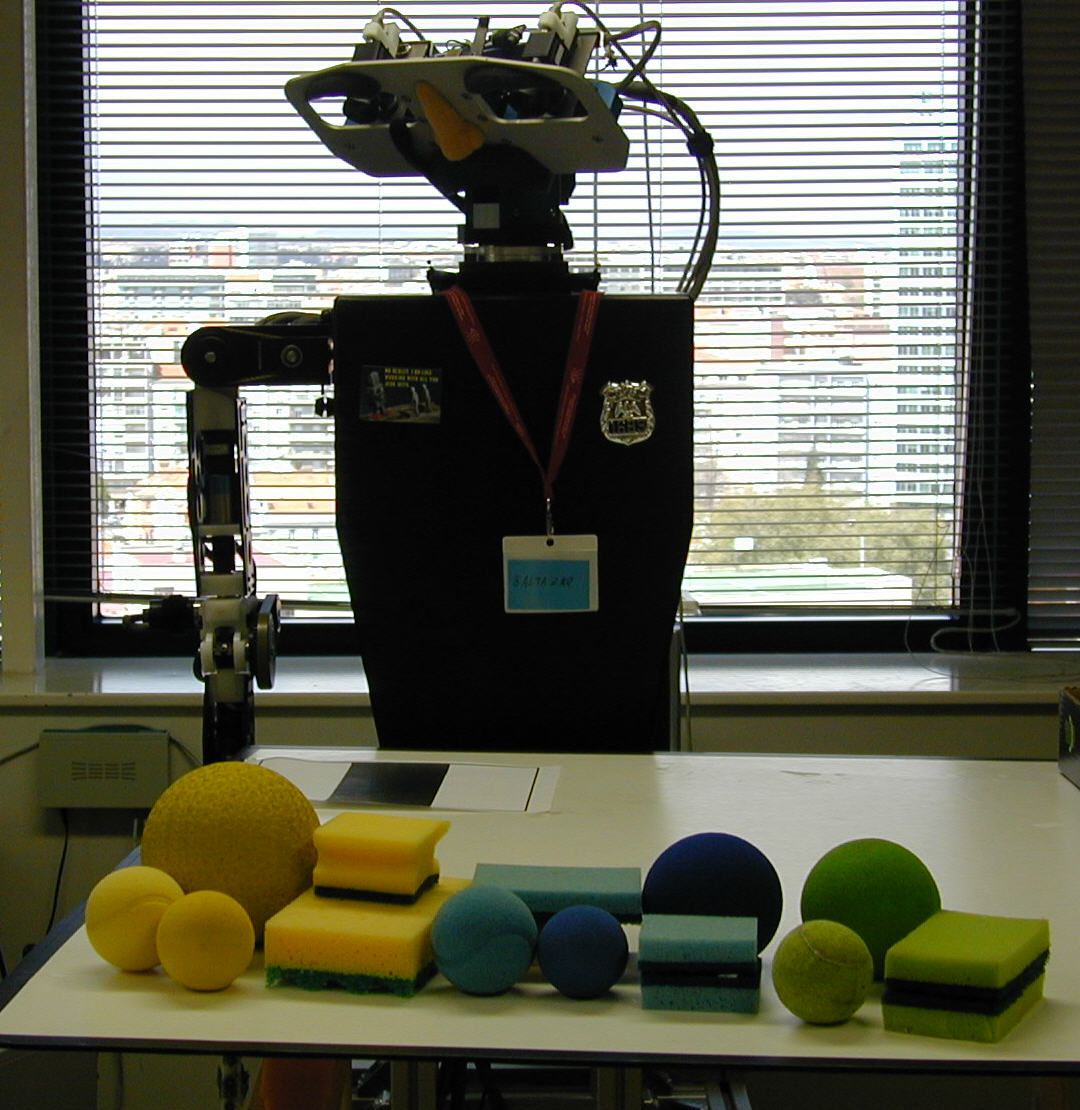
\includegraphics[width=0.546\textwidth]{montesano_setup} } \quad
%
\subfloat[][Objects being perceived and visually segmented by vision algorithms.]
{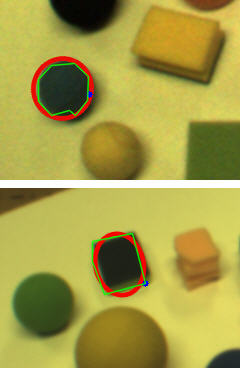
\includegraphics[width=0.364\textwidth]{montesano_shapeExample} }
\caption[Experimental setup of~\cite{montesano:2008}.]{Experimental setup of~\cite{montesano:2008}. In this work, a robot learns object affordances by autonomous exploration of colorful toys on a table; affordances are modeled as relationships between actions, objects and effects.}
\label{fig:montesano_setup}
\end{figure}

That work is influential in the cognitive robotics community, because it shows a computational model of affordances that is able to account for multiple possible affordances present in a robot's environment in a principled and probabilistic way, as opposed to assuming the existence of only one pre-defined affordance~(e.g., liftability).
In other words, this model is capable of learning multiple affordances present in the environment, or multiple possibilities offered by the objects perceived by the agent.
Computationally, it achieves this by using a \ac{BN} with a structure that encodes relations between motor actions, object features and resulting effects, as depicted in Fig.~\ref{fig:aff_models_intro:montesano}.

In a self-exploration manner (see Sec.~\ref{sec:motivation:devrob}), the Baltazar humanoid robot~\cite{lopes:2004:baltazar} tries out different motor actions onto different physical objects and records the observed effects, as shown in Fig.~\ref{fig:montesano_setup}.
Then, it learns the relations between the random variables involved (i.e., the variables pertaining to actions, object features and effects).
The actions are pre-defined tapping motions performed with the end effector, from four different directions.
The object features are (discretized) quantities related to size, shape, and color of objects extracted from vision.
The effects are the (discretized) physical displacements of the objects being moved on a tabletop, and the (discretized) durations of the contacts acquired with tactile sensors.
Data is discretized by using $k$-means clustering~\cite{lloyd:1982:kmeans} in order to train the \ac{BN} efficiently.

By repeating the exploration procedure several times, the robot acquires a set of~$N$ samples
\begin{equation}
    D = \{ y^{1:N} \},
\end{equation}
where the lower-case letter~$y$ represents the possible realizations~(i.e., values) of the random variable indicated by the upper-case letter~$Y$ (see Sec.~\ref{sec:background:theory:probability}).
Then, the set of nodes in a network,~$Y$, includes all of its variables, i.e., the ones representing robot actions~($A$), object features~($O$) and resulting effects~($E$), as follows:
\begin{equation}
    Y = \{ A, O_1,\dots,O_{n_O}, E_1,\dots,E_{n_E} \}.
\end{equation}

For the sake of this summary, let us assume for simplicity that the structure of the \ac{BN} is known, i.e., that we know the dependencies between the variables in~$Y$.

Given the (discrete) representation of actions, object features and effects, the authors use a \emph{multinomial distribution} and its corresponding conjugate, the Dirichlet distribution, to model the \acp{CPD} $p \left( Y_i \biggiven Y_{\parents(Y_i)}, \theta_i \right)$ and the corresponding parameter priors $p(\theta_i)$, respectively.
Let~$\mathcal{Y}_i$ and~$\mathcal{Y}_{\parents(Y_i)}$ indicate the range of values of random variables~$Y_i$ and the range of values of the parent nodes of~$Y_i$, respectively.
Assuming independence between the samples in~$D$, the marginal likelihood for the random variable~$Y_i$ and its parents given~$D$~(\cite{heckerman:1995:learnbn}) is:
\begin{align*}
p \left( y_i^{1:N} \biggiven y_{\parents(Y_i)}^{1:N} \right) &= \int \prod_{n=1}^n p \left( y_i^N \biggiven y_{\parents(Y_i)}^n, \theta_i \right) p(\theta_i) \, d\theta_i \\
 &= \prod_{j=1}^{|\mathcal{Y}_i|} \frac{\Gamma(\alpha_{ij})}{\Gamma(\alpha_{ij}+N_{ij})} \prod_{k=1}^{|\mathcal{Y}_{\parents(Y_i)}|} \frac{\Gamma(\alpha_{ijk}+N_{ijk})}{\Gamma(\alpha_{ijk})},
\end{align*}
where~$N_{ijk}$ counts the number of samples in which~$Y_i = j$ and~$Y_{\parents(Y_i)} = k$, $N_{ij} = \sum_k N_{ijk}$ and~$\Gamma$ represents the gamma function.
The \emph{pseudo-counts}~$\alpha_{ijk}$ denote the Dirichlet hyper-parameters of the prior distribution of~$\theta_i$ and $\alpha_{ij} = \sum_k \alpha_{ijk}$.
The marginal likelihood of the data is simply the product of the marginal likelihood of each node,
\begin{equation}
    p(D \given G) = p(Y^{1:N} \given G) = \prod_i p \left( y_i^{1:N} \biggiven y_{\parents(Y_i)}^{1:N} \right),
\end{equation}
where we have made explicit the dependency on the graph structure,~$G$.

One of the characteristics of Montesano's computational model of affordances is that it relies on discrete quantities being computed~(by a clustering algorithm) and passed as input to the \ac{BN}, rather than on the raw continuous-valued variables themselves.
In an extention work, Osório relaxes this assumption~\cite{osorio:2010:iros} in order to use the continuous values directly, by employing \acp{GMM} to represent the perceived visual features.
Results from a simulated environment suggest that continuous values can help \acp{BN} when data is noisy and when plenty of training data is available.
However, the practical applicability of this approach on real robots is problematic because of its
computational cost: the proposed solution uses the \EMlong~(\EM) algorithm, whose execution time is much slower than the one of Montesano's discrete \ac{BN} nodes.

Also, Montesano's model examines the possibilities afforded by \emph{one object}~at a time to the agent~(e.g., a ball affords high rollability).
In Ch.~\ref{chap:tool} we will extend the model in the context of \emph{tool use} affordances, meaning that, with exploration, the robot will learn to reason about two objects at a time, to be used as a tool and as an affected object, respectively~(e.g., a hammer and a nail).

\subsection{Affordances and Language}
\label{sec:background:previous_works:aff_language}

We have mentioned that robot affordances can help understanding a user's intention by recognizing the action performed by them.
Additionally, some works have used the concept of \emph{sensor fusion} to build \emph{multimodal affordances}, for example incorporating human language in addition to objects, where different modalities complement each other.

One of the first papers in this category is the one by Moratz~\cite{moratz:2008}, where linguistic instructions from a human to a robot are grounded in the affordances of objects present in a scene.
This system employs a robot object recognition system composed with a laser range finder, making use of an affordance-informed visual algorithm~(relating object shapes to object functionalities in a way pre-defined by the experimenter).
As a result, the system can be used to instruct a robot verbally, so that words relating to the affordances are mapped to the objects allowing the robot to choose the objects to use.
Notably, this setup requires a pre-defined set of known objects and of the rules associating affordances to objects.
Also, this approach does not exploit the information contained in nonverbal language, such as human gestures and movements.

\begin{figure}
    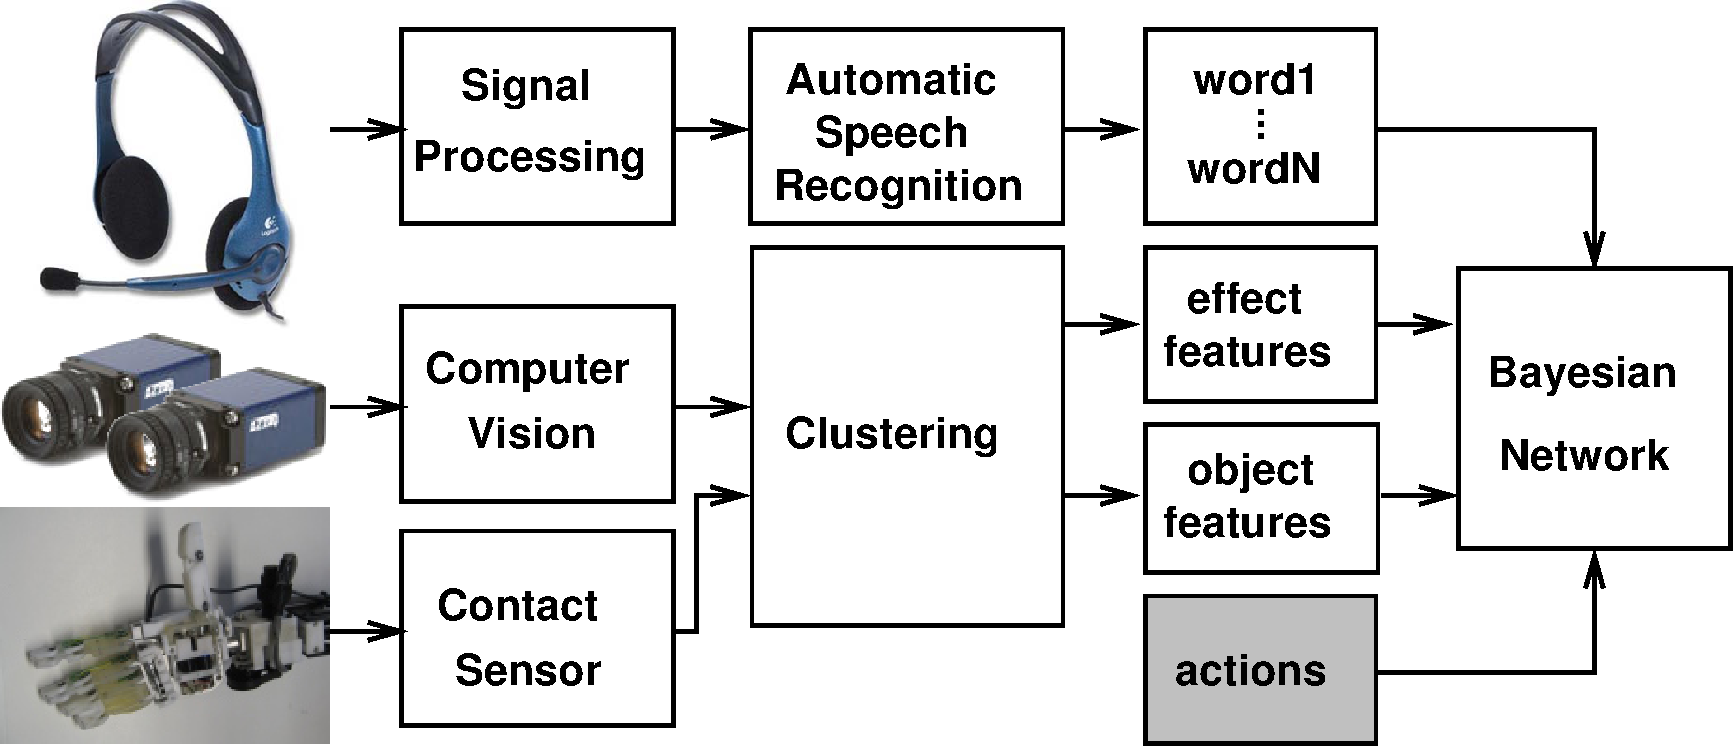
\includegraphics[width=0.9\textwidth]{salvi_scheme}
    \caption[Experimental setup of~\cite{salvi:2012:smcb}.]{Experimental setup of~\cite{salvi:2012:smcb}. In this work, which extends~\cite{montesano:2008}, a robot learns associations between \emph{spoken words} and object affordances~(where affordances are modeled as the relationships between actions, object features, effect features).}
    \label{fig:salvi_setup}
\end{figure}

A system with less stringent assumptions is the one by Salvi~\cite{salvi:2012:smcb}, whose experimental setup is shown in Fig.~\ref{fig:salvi_setup}.
In this work, building upon Montesano's model~(see Sec.~\ref{sec:background:previous_works:montesano}), object affordances are used to associate human words to the actual action, object and effect that they refer to.
Computationally, \acp{BN} are used, serving to learn \wordsmeanings{} associations.
This knowledge is then used together with spoken instructions for removing ambiguities during interactions with humans, for example permitting to command the robot to perform tasks.
We will expand upon the system by Salvi in Ch.~\ref{chap:gestures}.

Another work relating affordances and language is~\cite{celikkanat:2015:tamd}, which models the co-occurrence of actions, object information and language with a \emph{concept web} based on \acp{MRF}.
During operation, if partial information is available~(e.g., only the visual object information or the corresponding words), the corresponding affordance concepts previously learned are also activated.

\subsection{Reasoning about Human Actions}
\label{sec:background:previous_works:reasoning_about_human_actions}

Up to now, we have mentioned a number of works about robots that explore their environment, they operate on it~(e.g., using their limbs), and they build a cognitive model of the environment that takes into account the physical objects and the afforded actions.
Even though some of the works considered language, which is a human trait, the human dimension was not prominent in a physical or visual sense, meaning that the cognitive model used by the robot did not have any explicit representation of human users~(e.g., their location, their state, their physical action).
However, a growing line of research \emph{does} tackle this aspect, incorporating advances from other disciplines~(e.g., human activity recognition, machine learning and computer vision~\cite{aggarwal:2011}) onto robots.

Thus, we now list some works about autonomous robots possessing cognitive reasoning algorithms about environment objects \emph{and the humans} surrounding them.
This list is not exhaustive, but it is useful to understand the contributions of the next chapters.

\begin{figure}
\centering
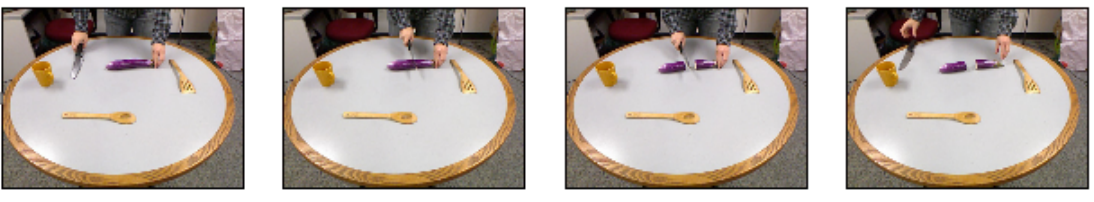
\includegraphics[width=0.9\textwidth]{aloimonos_eggplant}
\caption{Sequence of frames of a cutting action, reproduced from~\cite{pastra:2012:rstb}.}
\label{fig:minimalist_eggplant}
\end{figure}

Pastra and Aloimonos~\cite{pastra:2012:rstb} propose a ``minimalist grammar of action'' for robot cognition, linking the two aspects of language and action together.
That work is motivated by the biological evidence that both language and action are organized in a hierarchical, compositional way, and that the neural locus for composing their mechanisms is shared in Broca's area~\cite{pulvermuller:2005:broca}.
For example, Fig.~\ref{fig:minimalist_eggplant} shows a human person cutting an eggplant.
In order to do that, the person uses some prior knowledge and performs a sequence of low-level motor actions~(e.g., reaching for a knife tool, positioning the knife over the vegetable, exerting a vertical force to cut the vegetable, etc.), resulting in a high-level action~(e.g., cutting the vegetable).
In short, the proposed ``grammar'' is a formal, tree-like specification of actions with a biological human base.
This specification allows the development of generative computational models for action in the motor and visual space, by deploying a software component of a semantic memory~(i.e., the general human knowledge accumulated with experience) called the PRAXICON~\cite{pastra:2008:praxicon,mavroeidis:2016:praxicon}.
Indeed, this integration has been performed on a humanoid robot during the POETICON++ project\footnote{\url{http://www.poeticon.eu/} \label{footnote:poeticon++}}, and it will be described in detail in Ch.~\ref{chap:poeticon++_case_study}.

\begin{figure}
\centering
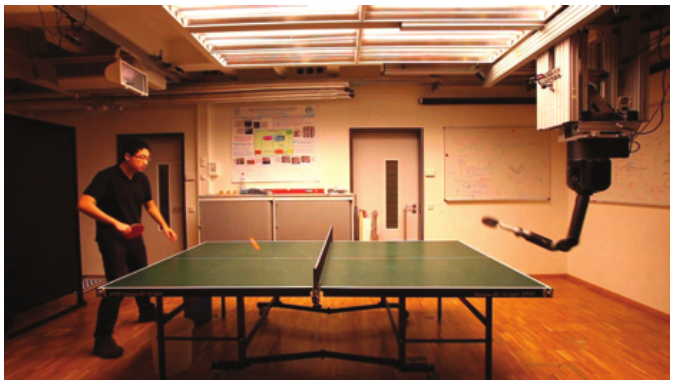
\includegraphics[width=0.9\textwidth]{wang2013-robot_table_tennis}
\caption{Tennis-playing robot, from~\cite{wang:2013:ijrr}.}
\label{fig:robot_table_tennis}
\end{figure}

In~\cite{wang:2013:ijrr}, a group from the Technical University of Darmstadt shows an example of a robotic system capable of recognizing and \emph{anticipating} a human's movements.
This system, shown in Fig.~\ref{fig:robot_table_tennis}, is capable of playing table tennis against a human opponent, using vision, control and machine learning.
It uses Gaussian Processes~\cite[p.~303]{bishop:prml}, finding a latent state representation of noisy and high-dimensional observations of human movement, at the same time capturing the dynamics of the motor task being considered.
Online approximate inference permits to anticipate the target position of the tennis ball~(i.e., the table region where the ball will fall) when the opponent performs the actual strike.
The predicted intention is then used to select the optimal robot hitting type~(e.g., forehand, middle, backhand strike).
This system requires specialized hardware, such as Gigabit Ethernet camera sensors with~200 frames per second.

\begin{figure}
\centering
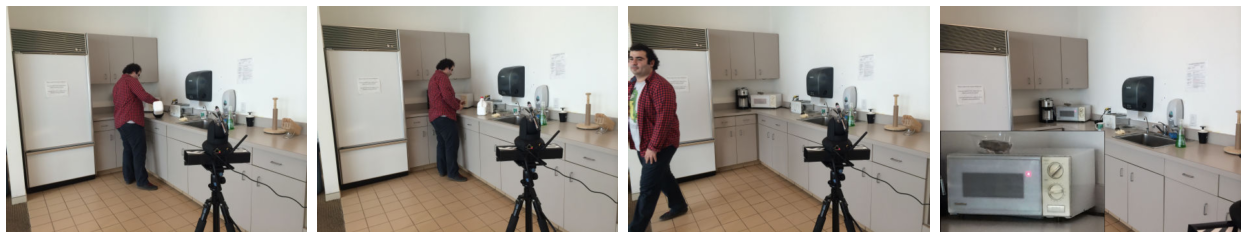
\includegraphics[width=0.9\textwidth]{wu2016watch-bot}
\caption[The Watch-n-Patch assistive robot system, reproduced from~\cite{wu:2016:icra}.]{The Watch-n-Patch assistive robot system, reproduced from~\cite{wu:2016:icra}. After spotting an unusual or incomplete action, the robot signals the information to the human user with a laser pointer.}
\label{fig:watchbot}
\end{figure}

The interest in vision techniques aimed at understanding human activity from videos has also grown~(e.g., using YouTube or other large video datasets).
In~\cite{wu:2015:cvpr}, a group by Cornell University propose a method to decompose complex events into simpler actions with video segmentation, and then learn the sub-action dynamics using an unsupervised graphical model, based on \acp{CRF} over Kinect~v2 data.
In~\cite{wu:2016:icra}, they then demonstrate how Watch-n-Patch\footnote{\url{http://watchnpatch.cs.cornell.edu/}}, an assistive robot with such a previously-trained system on board, can be useful not only to monitor daily human activities, but also to actively remind users of steps and pieces that they might forget in their typical activity sequences.
For example, they do that by using a laser pointer to indicate a ``forgotten'' object~(e.g., a milk carton) that was not handled appropriately after usage~(e.g., it was not put back in the fridge).

Koppula~\cite{koppula:2016:pami} consider the problems of detecting and anticipating human activities by combining complex full-body human trajectories, robot trajectories and object affordances knowledge in a graphical model based on \acp{CRF}.
That work shows that this kind of model can improve detection and anticipation over human action datasets.
The object affordances part in that model consists of a prior grounding specified by the programmer, assigning categories like ``drinkable'', ``pourable'', ``reachable'' to \actobj{} and \objobj{} relations, where the object features are \ac{SIFT}~\cite{lowe:1999:sift}.

The above ideas have also been explored in psychology, for example by Sciutti~\cite{sciutti:2015:fpsyg}, where the authors propose a model to make humanoid robots anticipate human partners' intentions, based on actively engaging humans in face-to-face interation and measuring the subtle kinematic movement signals that emerge.

\begin{figure}
\centering
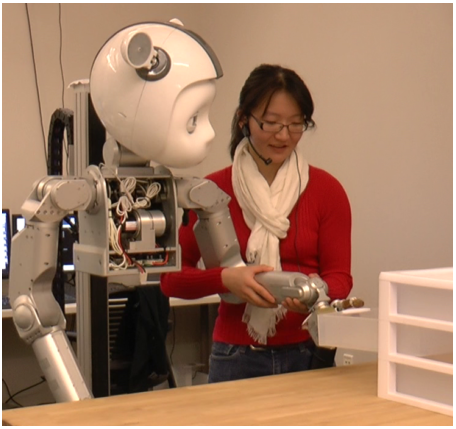
\includegraphics[width=0.6\textwidth]{chu_hri2016_curi}
\caption{A human guides a robot while it tries motor actions onto world objects to learn their affordances, from~\cite{chu:2016:hri}.}
\label{fig:chu_hri2016_curi}
\end{figure}

In~\cite{chu:2016:hri}, a group from Georgia Tech analyzes the impact of providing human guidance to a robot while it explores the environment and learns affordances~(see Fig.~\ref{fig:chu_hri2016_curi}), as opposed to having the robot learn them autonomously, like the approaches that we described so far.
In a controlled scenario with four household objects that a humanoid robot manipulates with different action parameters, they conclude that a mixed approach (i.e., partially human-guided, partially using self-exploration biased by information previously provided from human teachers) is effective for learning the affordances, requiring fewer interactions than other modalities.
A strong limitation of this approach is that it considers affordances as binary values~(i.e., does an object offer a specific affordance or not?) rather than probabilistically.
As previously mentioned, a probabilistic representation is key in modeling the inherent noise in uncontrolled, human environments.

\bigskip

In this chapter, we have provided the fundamental information needed to understand the contributions of the thesis in the next chapters.
Specifically,
we have gone through some theory~(\aclp{BN}) and
we have listed relevant works related to the broad scope of the thesis.


%!TEX encoding = UTF-8

\chapter{Experimental Platform}
\label{chap:platform}

In this chapter, we provide the practical groundwork for the experiments described in the thesis.

We start by describing the iCub humanoid robot in Sec.~\ref{sec:platform:icub}.
Then, in Sec.~\ref{sec:platform:scenario} we illustrate the experimental scenario adopted in the experiments.
Finally, Sec.~\ref{sec:platform:software_architecture} presents our modular system for robot affordance learning, based on autonomous robot exploration of the world and visual processing.
The whole system will be used as a building block for the next chapters.

%%%%%%%%%%%%%%%%%%%%%%%%%%%%%%%%%%%%%%%%%%%%%%%%%%%%%%%%%%%%%%%%%%%%%%%%%%%%%%%%
\section{The iCub Humanoid Robot}
\label{sec:platform:icub}

\begin{figure}
\centering
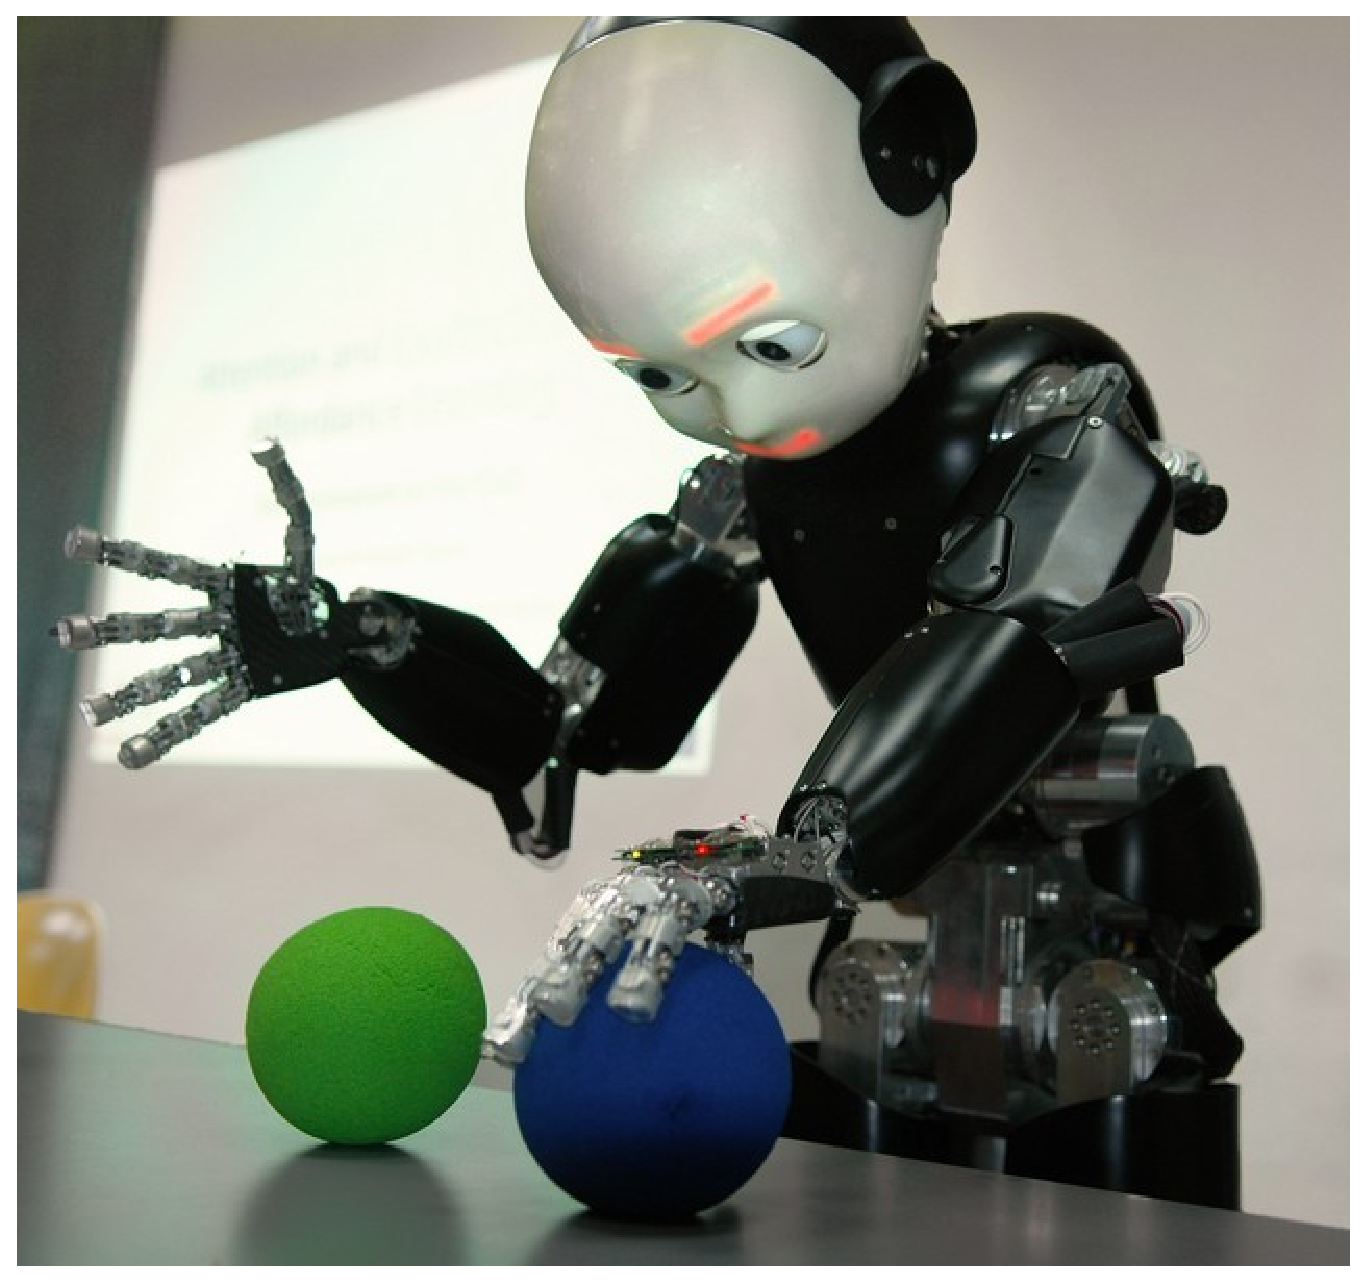
\includegraphics[width=0.9\textwidth]{icub_green_blue_balls}
\caption[The iCub humanoid robot.]{The iCub humanoid robot (picture by Lorenzo Natale).}
\label{fig:icub}
\end{figure}

In this section, we illustrate the humanoid \emph{robot} that we will use to run the experiments of this thesis.

The robot that we use is the \emph{iCub} child-like robot~\cite{metta:2010:nn}, shown in Fig.~\ref{fig:icub}.
Its shape is similar to that of a 5-year-old child, with a height of 1~meter, a weight of~27 kilograms, and a head with fully articulated eyes~\cite{beira:2007:msc}.
The structure of the iCub is sophisticated: it has a high number of \acp{DoF}\footnote{%
At the time of writing this thesis, the iCub robot is the second humanoid robot with the highest number of \ac{DoF} (53~\ac{DoF}), being surpassed only by the ARMAR robot by Karlsruhe Institute of Technology (63~\ac{DoF}) \cite{asfour:2019:armar_family}.}% end footnote
, the majority of which are located at the arms and hands, in order to make the robot perform object grasping, dexterous manipulation as well as articulatory gestures.
The iCub also has tactile sensors and microphones: these robot sensors are not directly used in this thesis, however they are included and used in some previous studies (\cite{montesano:2008,salvi:2012:smcb}) related to this thesis.
It is an \emph{open-source platform}, having been adopted by more than~30 research groups and universities worldwide~\cite{natale:2019:icub_bookchapter}.

The open-source iCub software is, as such, the work of a large community\footnote{\url{http://www.icub.org/}, \url{https://github.com/robotology}}:~2 million \ac{LoC}, hundreds of contributors\footnote{\url{https://www.openhub.net/p/robotology}}.
Parts of the available software can be used in other applications and platforms~(i.e., without the iCub), for example the visual processing algorithms.
iCub software modules, such as the ones developed for this thesis, rely on the \ac{YARP} middleware~\cite{metta:2006:yarp,fitzpatrick:2014:yarp}.
\ac{YARP} is similar to \ac{ROS}\footnote{%
At the time of writing this thesis, \ac{ROS} \cite{quigley:2009:ros} is the \defacto{} standard middleware in robotic research.
}, % end footnote
following the same \emph{middleware} concepts about managing distributed computations across a cluster of heterogeneous computers, hardware abstractions, low-level device drivers, message passing between processes, and implementation of commonly used functionality (e.g., geometry, linear algebra, vision algorithms).

The iCub robot was developed for studying cognition and learning.
The main idea behind this platform is that it is born with simple skills, and then it can become intelligent over time by interacting with the enviroment, where the term intelligence encompasses manipulation, social skills, and interactive skills.
As a result, it can gain a certain degree of autonomy.
The usefulness of the iCub is in its completeness: it encompasses movement~(high number of motors) and the possibility to measure the external environment~(sensors), which in turn permit to study aspects of higher intelligence~(algorithms).

%%%%%%%%%%%%%%%%%%%%%%%%%%%%%%%%%%%%%%%%%%%%%%%%%%%%%%%%%%%%%%%%%%%%%%%%%%%%%%%%
\section{Experimental Scenario}
\label{sec:platform:scenario}

\begin{figure}
\centering
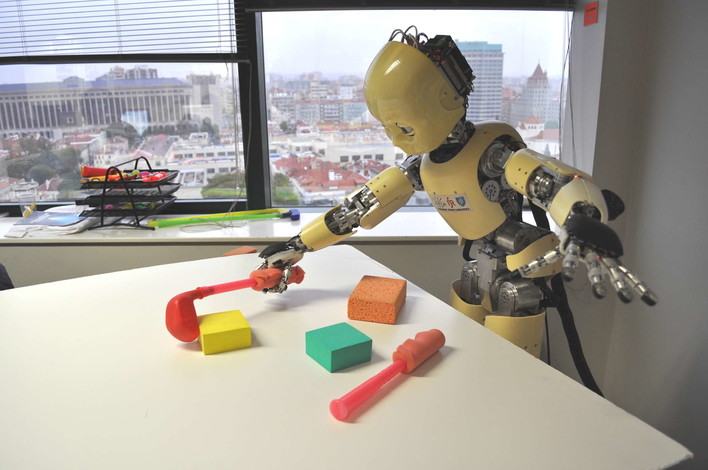
\includegraphics[width=0.9\textwidth]{icub_playing_with_objects_icdl-epirob2014}
\caption[The iCub robot in a playground table scenario.]{The iCub robot in a playground table scenario. Objects and tools are present in the scenario, so that the robot can interact with them, it can acquire a model of the environment derived from sensorimotor data, and it can use such a model for reasoning about the environment.}
\label{fig:icub_playing_with_objects}
\end{figure}

In our scenario, the iCub robot is positioned next to a \emph{playground table}, meaning a table which can have one or more objects on top of it.
Examples of these objects are colorful toys, sponges and elongated tools.
This scenario is designed so that the robot interacts with the objects, it acquires the model of the environment from sensorimotor data, and it can then use the acquired knowledge for reasoning about the environment.
Fig.~\ref{fig:icub_playing_with_objects} shows an example of our scenario.

In following Montesano's approach (see Sec.~\ref{sec:background:previous_works:montesano}), the variables that our model considers are related to: action, object, and effect.

Note that, when a robot interacts with its environment autonomously in a self-exploration fashion, several variables can be actively chosen by the robot, for example the motor action and the target object.
In our case, these variables are usually interventional~(see p.~\pageref{para:interventional_vars}), being set to their specific value during each experiment by the experimenter or by the robot.

\begin{figure}
\centering
\subfloat[][Grasp.]
{ 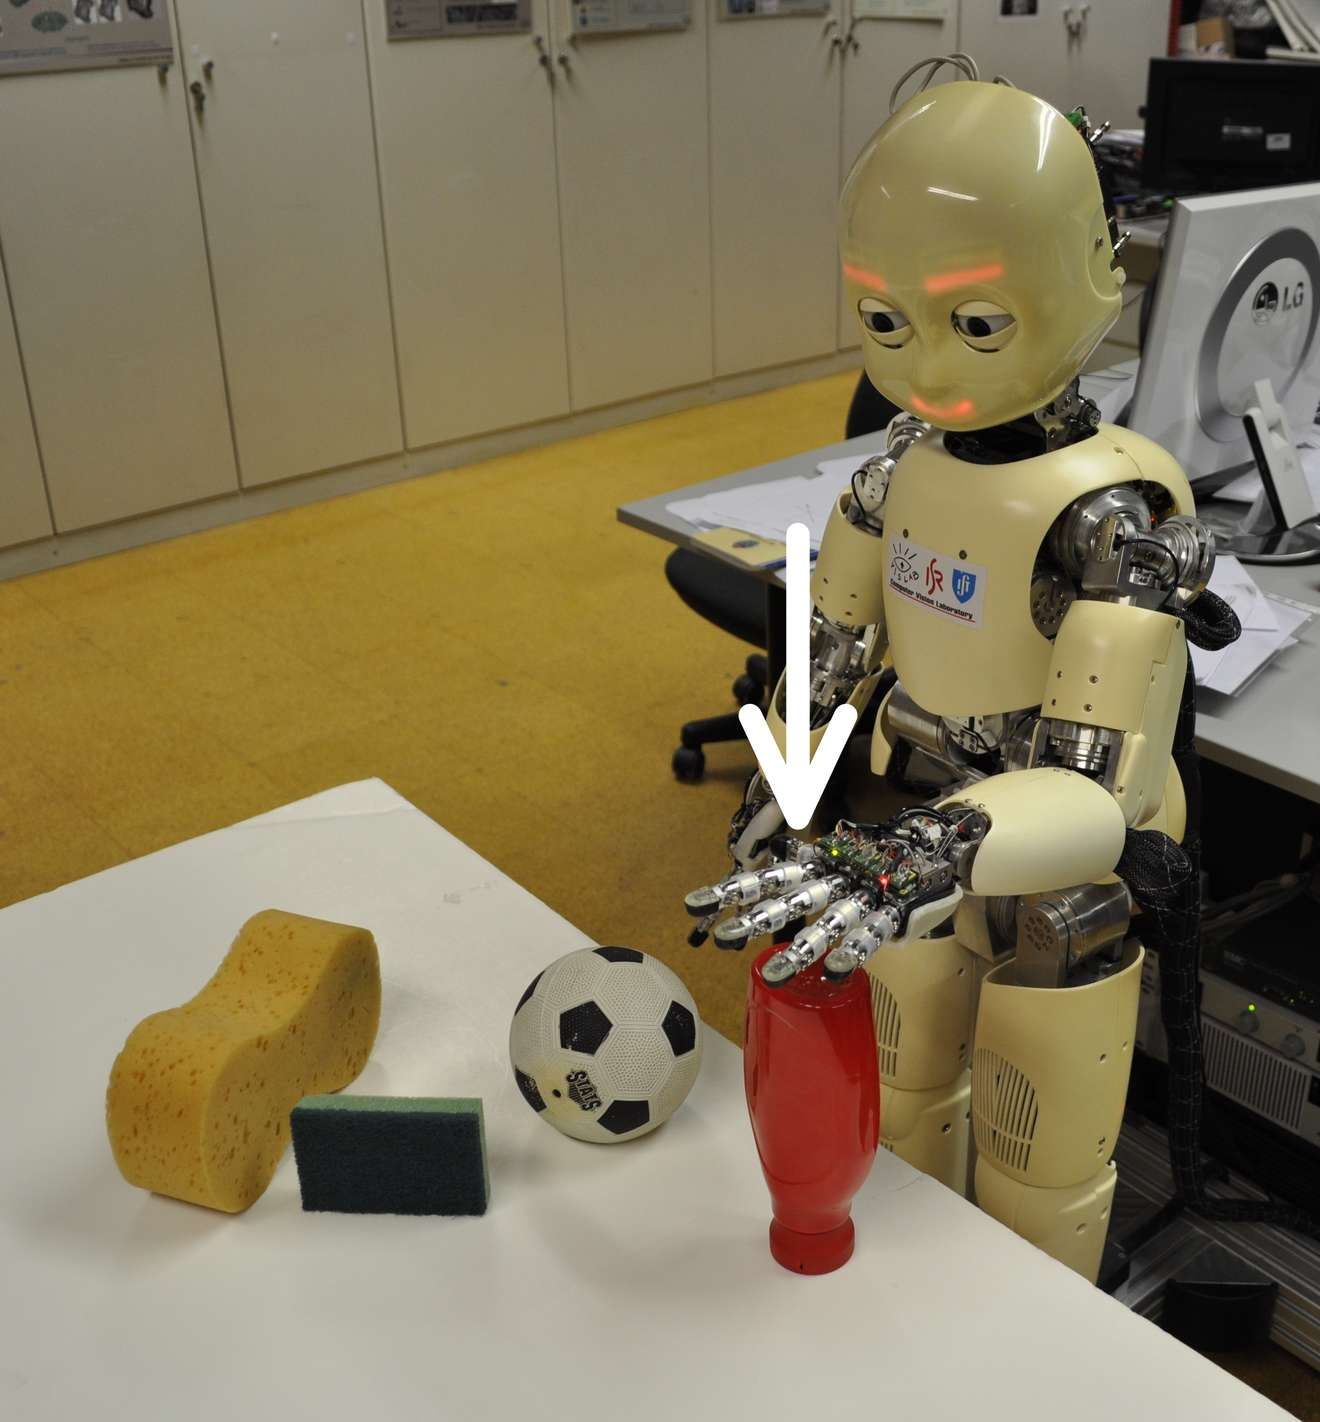
\includegraphics[width=0.25\linewidth]{icub_motor_actions_grasp_lowqual} } \quad
%
\subfloat[][Tap.]
{ 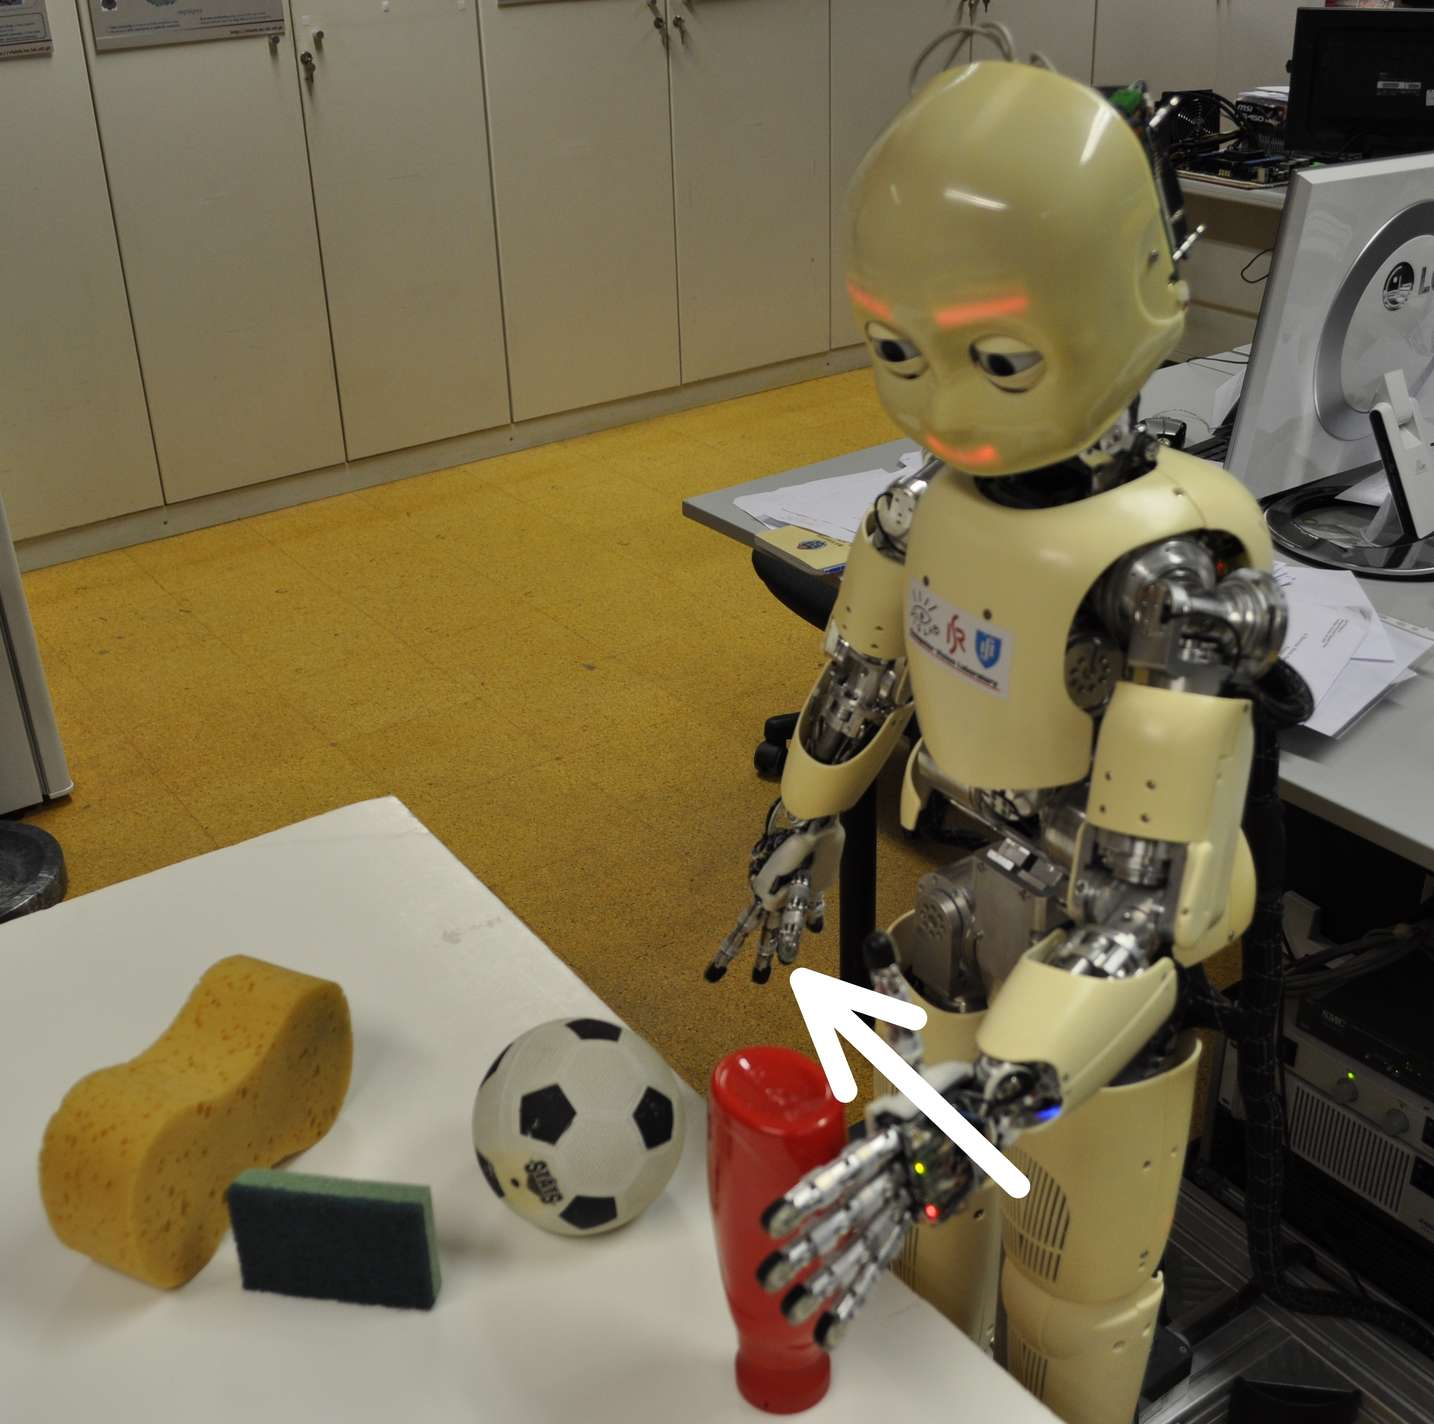
\includegraphics[width=0.27\linewidth]{icub_motor_actions_tap_lowqual} } \quad
%
\subfloat[][Push.]
{ 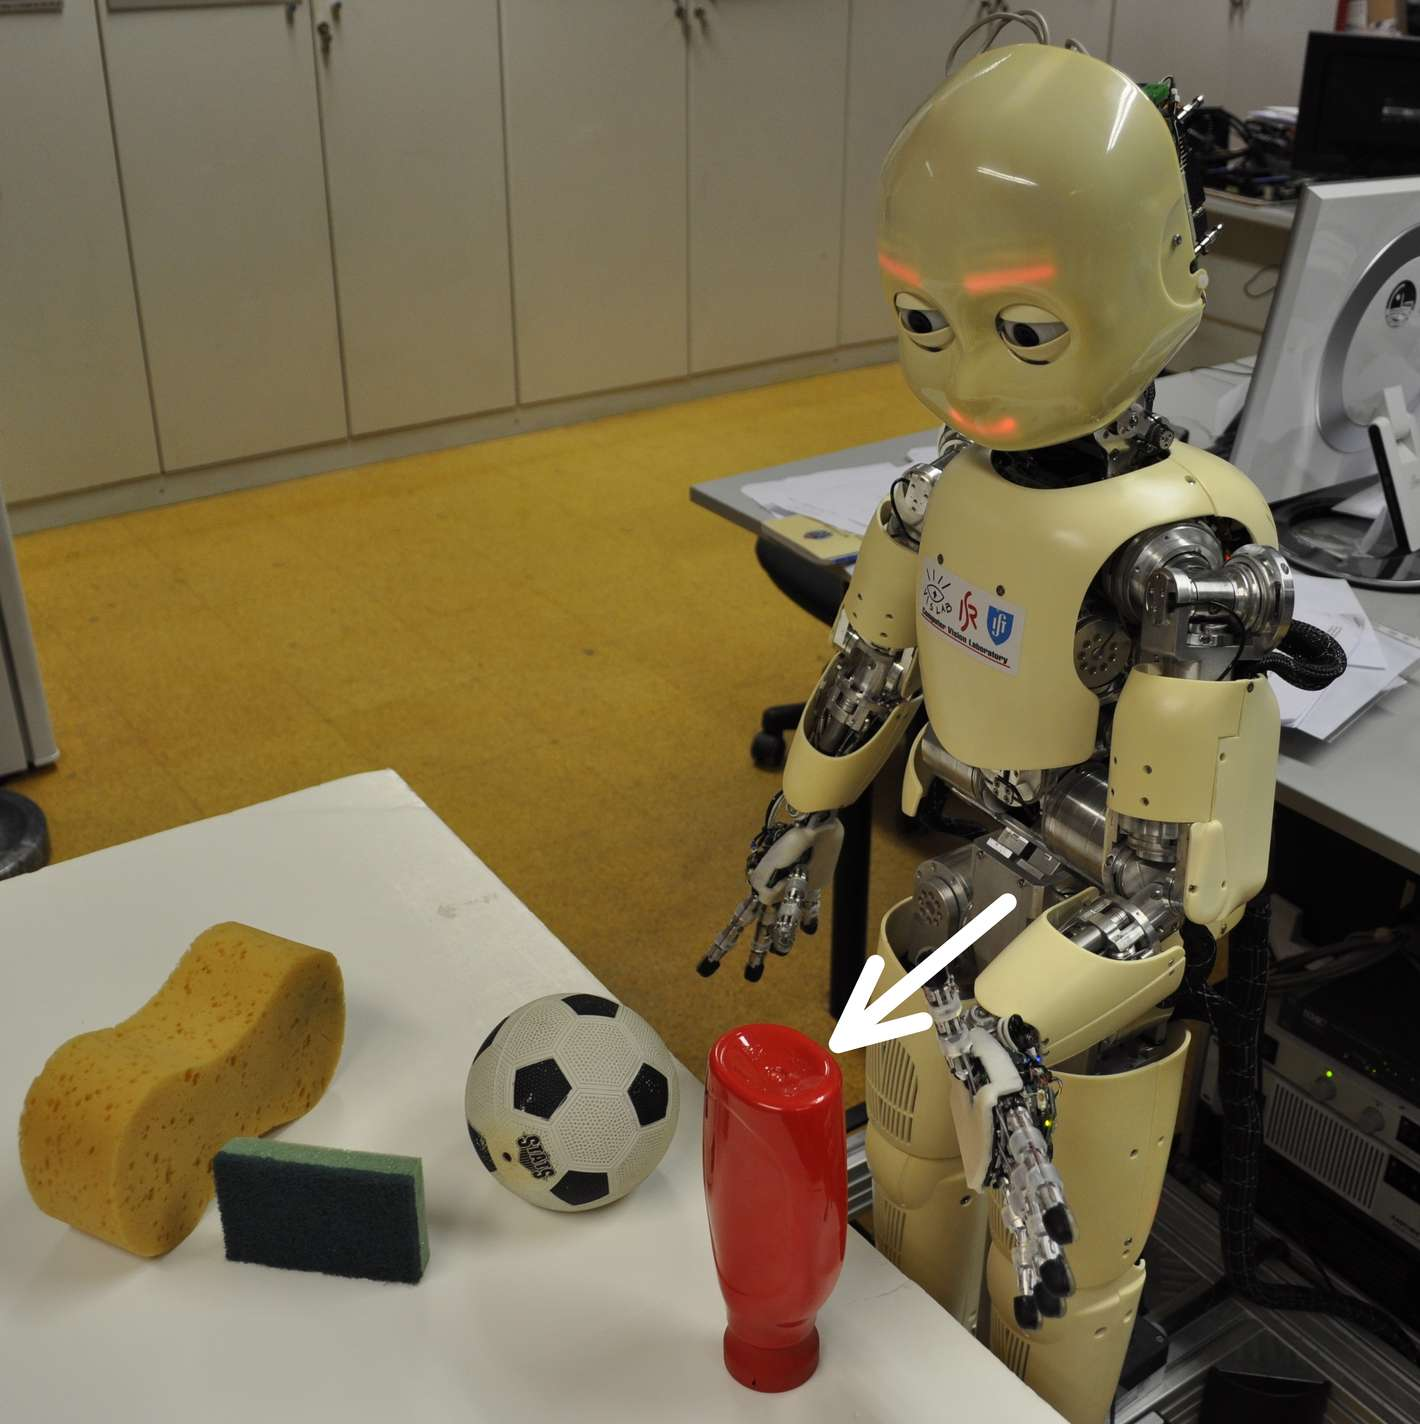
\includegraphics[width=0.27\linewidth]{icub_motor_actions_push_lowqual} }
%
\caption{Examples of manipulative motor actions performed by the iCub robot onto environment objects.}
\label{fig:icub_motor_actions}
\end{figure}

Regarding the motor \emph{actions} that can be executed by the iCub during experiments, in this thesis we consider manipulative hand gestures.
These are movements performed by the \armhand{} chain of the robot, capable of touching objects in the environment from different directions.
Fig.~\ref{fig:icub_motor_actions} shows some examples of these motor actions, highlighted in white.

In this thesis, the low-level control routines to realize the motor behaviors on the iCub robot (both simulated and real) are based on works and software modules previously made available by other researchers in the iCub community~\cite{pattacini:2010:iros,roncone:2016:rss}.

Regarding the \emph{effects} in the environment that are measured using robot perception, we consider physical displacements of objects on the table, being moved by the effector of robot from the time when the robot performs the action, until a pre-defined fixed duration (number of frames) afterwards. \label{para:effects}
The effector can be the agent's bare hand or the tip of a grasped tool, as we will describe in Ch.~\ref{chap:tool}.
The physical displacement of an object is computed as the difference between the final and initial coordinates of that object on a table.
Furthermore, we consider two displacement effects: along the lateral and longitudinal direction, respectively.
By clustering the continuous sensory values, we define five discrete levels for these effects: Very Positive (VP), Low Positive (LP), No Movement (NM), Low Negative (LN) and Very Negative (VN).
These levels correspond to an object moving
\begin{itemize}
\item VP: significantly to the left (or front) from the robot's perspective;

\item LP: slightly to the left (or front);

\item NM: little or no movement;

\item LN: slightly to the right (or back);

\item VN: significantly to the right (or back).
\end{itemize}

Recall from p.~\pageref{para:BN_causality_clarification} that \acp{BN} offer the possibility of representing causal relationships, based on knowledge (specified by the experimenter arbitrarily) of the world domain being modeled.
In the experimental part of this thesis, the robot chooses an action~$A$, it executes it on an object (with certain features) $O$, and it ``causes'' the effect~$E$ as a consequence.
Since $A$ and~$O$ are given as priors, and since effects happen later in time, we attribute the meaning that $A$ and~$O$ are causes, whereas $E$ are consequences.
Still, from the point of view of \acp{BN}, $A$, $O$ and $E$ are variables with no temporal information.
In this sense, as clarified in Sec.~\ref{sec:background:theory:graphical_models}, the model does not learn causal relationships.

%%%%%%%%%%%%%%%%%%%%%%%%%%%%%%%%%%%%%%%%%%%%%%%%%%%%%%%%%%%%%%%%%%%%%%%%%%%%%%%%
\section{Software Architecture}
\label{sec:platform:software_architecture}

In this section, we introduce our software framework that permits robots to sense, learn, and use the information contained in surrounding objects as well as their affordances.
It is a modular software framework for experiments in visual robot affordances, directed at the robotics, psychophysics and neuroscience communities.
Although the system was developed for the iCub platform in particular, thanks to its modular nature, parts of the system can be used for other robots.
We make this framework publicly available\footnote{\url{https://github.com/gsaponaro/robot-affordances} \label{footnote:robot-affordances_url}}.
Below, we show how this system can be used for
(i)~the perception of relevant visual features of a robot's surrounding objects;
(ii)~reasoning about the affordances of those objects and, as a result,
(iii)~supporting the new capabilities and behaviors described in the next chapters, for example tool use and action planning.

The basic intuition behind our architecture is that a robot learns links between object shape features and their physical properties: for instance, the notion that spherical objects roll faster than cubic ones when pushed laterally with an effector~(e.g., a robot hand or a tool held in the robot's hand).

Because learning is based on a \emph{probabilistic model}, the approach is able to deal with uncertainty, redundancy and irrelevant information.
We say that affordances are learned, because we let the robot discover them from autonomous experience in its environment, and then use the learned model in various profitable ways, e.g., prediction, tool use learning, planning a sequence of actions to achieve complex goals such as stacking objects.

As mentioned in Ch.~\ref{chap:background}, Zech published a systematic taxonomy of robot affordance models~\cite{zech:2017:ab}.
According to their criteria (defined in their taxonomy),
in terms of \emph{perception} the works in this thesis classify as using an agent perspective, meso-level features, first order, stable temporality (i.e., related to static object properties that do not change over time, such as the shape of rigid objects).
In terms of \emph{development}: acquisition by exploration, prediction by inference, generalization exploitation by action selection and language, and offline learning.

\subsection{Visual Pipeline}
\label{sec:platform:software_architecture:visual_pipeline}

\begin{figure}
    % align option is for linebreaks, https://tex.stackexchange.com/a/124114
    % RGB color is light gray
    \tikzstyle{block} = [rectangle, draw, thick, align=left, fill={rgb,255: red,234; green,236; blue,239}]
    %
    \centering
    \resizebox{0.9\textwidth}{!}{ % https://tex.stackexchange.com/a/363884
    \begin{tikzpicture}
    \node (robot_cam) [draw=none, circle, minimum size = 1mm, align=left] at (0, 0) {robot \\ camera};
    \node[draw=none, label={\tiny color image}, text width=1.25cm] (inv1) [right=of robot_cam, xshift=-0.75cm] {};
    \node[block, right=of inv1, xshift=-0.75cm] (segm) {segmentation};
    \node[draw=none, label={\tiny binary image}] (inv2) [right=of segm] {};
    \node[block, right=of inv2] (bd) {Blob \\ Descriptor};
    \node[block, below=of inv2] (sl) {Sequential \\ Labeler};
        \node[block, right=of bd] (bn) {Bayesian \\ Network \\ affordance \\ knowledge};
    %
    \draw[affarrow] (robot_cam) -- (segm.west);
    \draw[affarrow] (inv2.center) -- (sl.north);
    \draw[affarrow] (segm) -- (bd);
    \draw[affarrow] (sl) -| node[above, text width=1.25cm, xshift=-0.4cm]{\tiny labeled image} (bd);
    \draw[affarrow] (bd) -- node[above, text width=1.25cm, xshift=0.1cm, yshift=0.5cm]{\tiny shape features} (bn);
    \draw[->, dotted] (inv1.center) |- ([shift={(0mm,-26mm)}]inv1.center) -- node[below]{\tiny (optional connection, for visualization purposes)} ([shift={(0mm,-20mm)}]bd.south) -| ([shift={(5mm,0mm)}]bd.south);
    %
    \draw ([shift={(3mm,14mm)}]segm.north east) to[out=-90,in=0,distance=3.5cm] ([shift={(-5mm,-20mm)}]inv1.south);
    \node[text width=3.4cm, align=right] at (3.5, 1.4) {\small \emph{existing work by other researchers} \tiny (see p.~\pageref{para:lbpExtract})};
    \node at (7.3, 1.4) {\small \emph{our contributions}};
    \end{tikzpicture}
    } % end resizebox
    \caption[Our pipeline for computing visual affordance features.]{Our pipeline for computing visual affordance features. Boxes indicate software modules, arrows indicate data flow connections, dotted arrows indicate optional data flow connections.
    See text for details, and Fig.~\ref{fig:shape_features_pipeline} for an example computation.}
    \label{fig:our_aff_pipeline}
\end{figure}

\begin{figure}
\centering
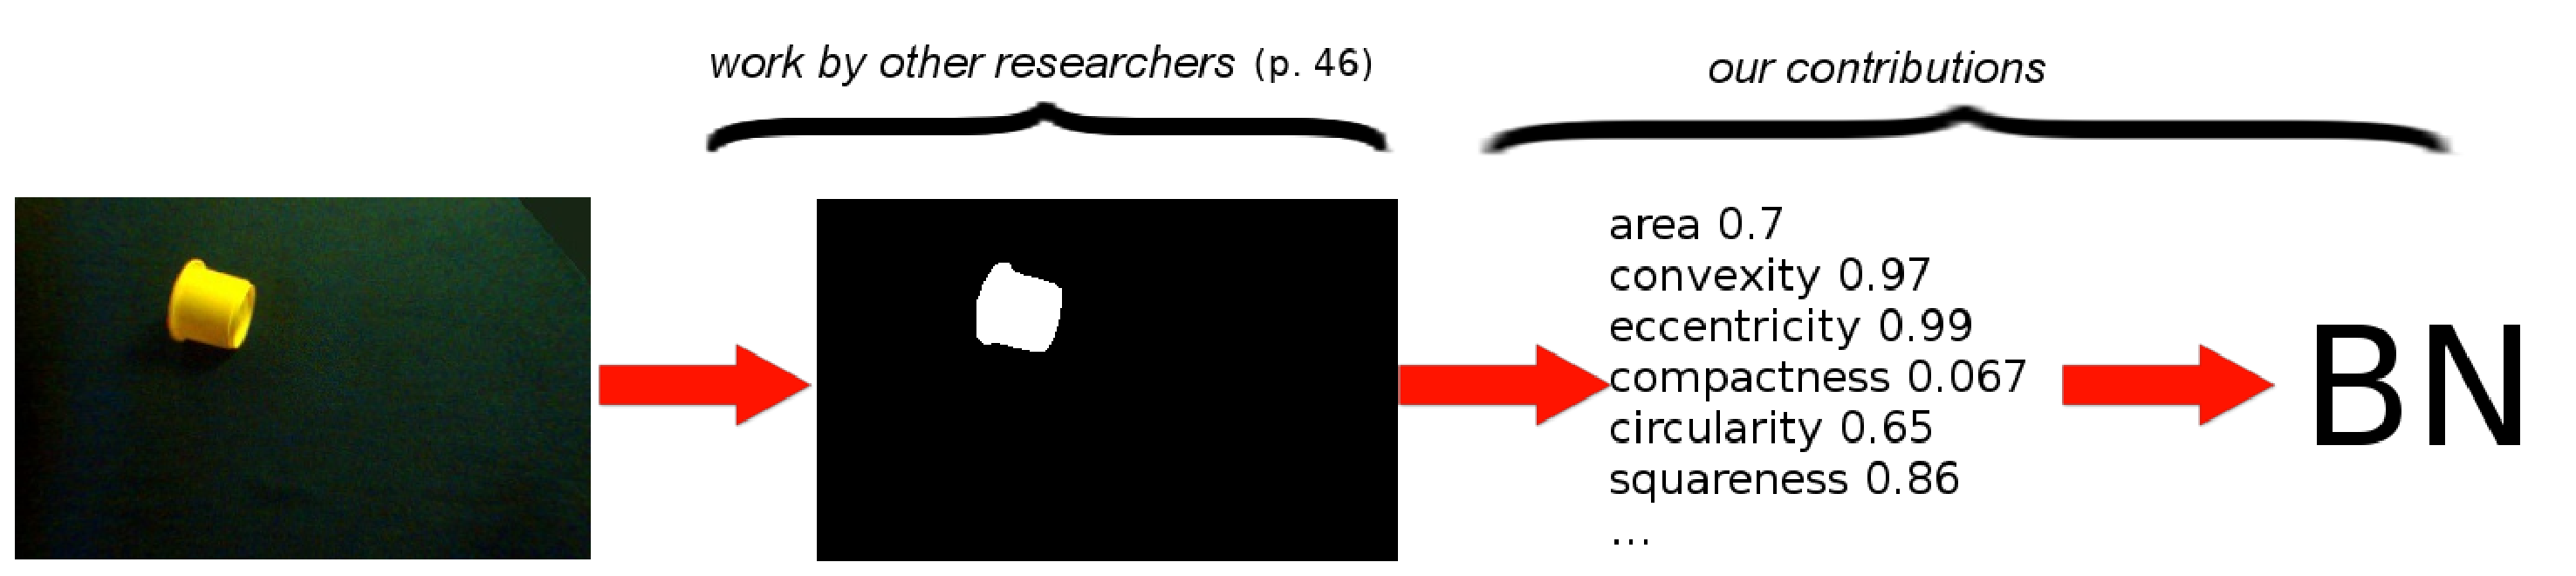
\includegraphics[width=0.9\textwidth]{shape_features_pipeline3_link_to_p46}
\caption[Example computation of extracting salient shape features for affordances.]{Example computation of extracting salient shape features for affordances.
From left to right: robot camera color image, binary segmentation image, shape features, \acl{BN} affordance knowledge.
The set of extracted shape features characterizes the object.
This set is then used to train the robot affordance knowledge model, and to perform inference queries on an affordance database.
See also Fig.~\ref{fig:our_aff_pipeline} for the diagram of software modules.}
\label{fig:shape_features_pipeline}
\end{figure}

The objective of this section is to illustrate a real-time~(30 fps), versatile and easy-to-use visual processing software that can be used in different scenarios such as robot perception, higher-level cognitive reasoning~(e.g., reasoning about the possibilities afforded by perceived objects) and related studies.

Starting from the beginning of such a perception and reasoning pipeline, let us first focus on visual features.
Computing features of interest of objects present in images is a frequent task in cognitive robotics.
For example, for the iCub humanoid robot this fundamental capacity was required during the research projects RobotCub\footnote{\url{http://www.robotcub.org/}} and POETICON++\footref{footnote:poeticon++}, where the robot had to see, characterize and grasp objects located on a playground table scenario, as described in Sec.~\ref{sec:platform:scenario}.
The exact requirements and subtleties vary slightly among different projects, setups and demonstrations.

Recall from Sec.~\ref{sec:motivation:neuro:twostreams} that the two-streams hypothesis of neuroscience speculates that visual perception occurs across two separate pathways: ventral and dorsal.
The former is mainly related to object recognition and categorization, the latter guides object-directed actions~(e.g., reaching and grasping).
We now illustrate the main components of our robot affordance pipeline, which is inspired by the dorsal pathway, in the sense that it does not require to know or recognize the category of objects, instead it reasons on their low-level shape features, and it permits the agent to act fast.

Fig.~\ref{fig:our_aff_pipeline} shows the organization of our pipeline, where boxes indicate conceptual~(and software) modules, arrows indicate data flow connections, and dotted arrows indicate optional data flow connections.
Fig.~\ref{fig:shape_features_pipeline} shows an example computation.
At the end of the pipeline, shape features are computed.
They serve as the data (about world objects) for the \ac{BN} computational implementation of the affordance knowledge.
In particular, using clustering of the continuous sensory values, we define three discrete levels for each shape feature: Low~(L), Medium~(M), and High~(H). \label{para:objects}

\begin{table}
\caption{Shape descriptors.}
\label{tab:descriptors}
\centering
\begin{tabular}{lp{0.6\columnwidth}}
\toprule
descriptor & definition \\
\midrule
area & number of blob pixels, normalized w.r.t. a constant \\
convexity & ratio between convex hull perimeter and object perimeter \\
eccentricity & ratio between minor and major axes of best-fit ellipse \\
compactness & ratio between object area and squared external contour perimeter \\
circularity & ratio between object area and area of minimum-enclosing circle \\
squareness & ratio between object area and area of minimum-enclosing rectangle \\
convexity defects & number of ``holes'' along blob contour \\
image moments & weighted averages of the blob pixels' intensities \\
\bottomrule
\end{tabular}
\end{table}

The modules are the following:
\begin{description}
    \item[segmentation] A visual module that takes as input a color image obtained from a robot camera, and outputs a binary image containing white pixels on the location of the objects, black pixels elsewhere~(i.e., background).
    Because the overall architecture is modular, it is possible to plug and play different segmentation implementations and algorithms as this module, provided that they have the required input and output format.
    The implementation that we adopt for the experiments in this thesis~(written by other researchers\footnote{%
        \texttt{lbpExtract} software module, written by Vadim Tikhanoff and available at \url{https://github.com/robotology/segmentation}
    }) % end footnote
    uses \acp{LBP}~\cite{ojala:2002:pami} for analyzing the texture of objects on a table in front of the robot, based on comparing the intensity of each pixel with its neighbors and representing this relationship with a histogram of binary numbers. \label{para:lbpExtract}

    \item[Sequential Labeler] A visual module that takes as input a binary segmentation image, and extracts as output the connected components contained therein (i.e., contiguous subsets of pixels). We call the output image \emph{labeled}, meaning that its pixels correspond to identifiers of the segmented objects: pixels are set to zeros over the background, to ones over the first segmented object, to twos over the second segmented object, etc.

    \item[Blob Descriptor] A visual module that, from the binary and labeled images, computes a vector of descriptors for each segmented object present in the scene.
    This module performs measurements on the connected components~(obtained by the two modules above), in order to extract some of their salient characteristics.
    The features that we extract are pre-categorical shape descriptors~\cite{zhang:2004:shape} computed as geometric relationships between perimeter, area, convex hull and approximated shapes of the segmented silhouettes of the objects in front of the robot.
    We list these shape descriptors in Table~\ref{tab:descriptors}.
\end{description}

The different types of images being processed and passed along between the modules are:
\begin{description}
    \item[color image] as acquired from the robot camera driver;

    \item[binary segmentation image,] which separates the objects of interest from the background. This image thus contains the contours of the object shapes, which we call \emph{blobs};

    \item[labeled image,] containing the uniquely-numbered connected components corresponding to the visual blobs: the pixels of the~$i^{\text{th}}$ blob are numbered~$i$, the background pixels are numbered zero.
\end{description}

\subsection{Impact}
\label{sec:platform:software_architecture:impact}

In addition to being applied for this thesis and other works authored by \myFullName, our visual affordances system has also been used by external researchers outside our scope,
namely:
\begin{itemize}
    \item in a developmental psychology work that links the visual appearance of objects with language learning on an iCub robot~\cite{morse:2016:cogsci}, and

    \item in studies about robot tool affordances which rely on the \emph{deep learning} paradigm instead of \aclp{BN}~\cite{dehban:2016:eccvws,dehban:2016:icra,dehban:2017:humanoids}.
\end{itemize}


%!TEX encoding = UTF-8

\chapter{Affordances, Gestures and Language}
\label{chap:gestures}

In this chapter, we present a computational model (see Fig.~\ref{fig:gestures:gestures_lang_computational_model}) that combines object affordances with communication, and we show the benefits of such an approach in cognitive robotic systems.

\begin{figure}[h]
\newcommand{\myscaleaffmodels}{0.7}
\centering
\begin{tikzpicture}[scale=\myscaleaffmodels, every node/.style={transform shape}]
\montesanoAE
\montesanoO
\saponaroGestRecBox
\salviW
\end{tikzpicture}
\caption{Computational model of affordances with gestures and language.}
\label{fig:gestures:gestures_lang_computational_model}
\end{figure}

We consider two aspects of communication: nonverbal (i.e., body gestures) and verbal (i.e., language).
It is worth exploring both of these modalities in robots, as means for providing them the skills to engage in sociality and collaboration with humans.
In other words, communication is useful for becoming social\footnote{A social robot is ``[a robot that is] able to communicate and interact with us, understand and even relate to us, in a personal way. [It] should be able to understand us and itself in social terms''~\cite{breazeal:2002:dsr}.}.
By incorporating communication aspects into a cognitive robotic system, we permit the leap from ego-centric behavior~(where the robot explores its surrounding world) to a social one~(where the robot perceives the actions of other agents and links them to its own actions).

Regarding nonverbal communication, we focus on human \emph{gestures} perceived with vision sensors.
We developed a gesture recognizer for manipulative hand gestures.
This recognizer receives a sequence of camera images depicting a person making manipulative gestures (these images contain the \emph{gesture feature} inputs), and it produces a probability distribution
over the gesture being recognized as output\footnote{Implementation details about the gesture recognition model will be given in Appendix~\ref{chap:gesture_recognition}. \label{footnote:link_to_appendix_gest_rec}}.

We embed the gesture recognizer into a computational model of object affordances, permitting to extend previous works (\cite{salvi:2012:smcb}, see also Sec.~\ref{sec:background:previous_works:aff_language}).
With our combination of affordances and gestures we show that, after having acquired knowledge of its surrounding environment from autonomous exploration, a humanoid robot can generalize this knowledge to the case when it observes another agent~(human partner) performing the same motor actions previously executed by the robot during training.
This is the shift from reasoning purely about actions performed by the robot itself~(ego-centric phase) to reasoning about actions performed by external human users~(social phase).

We also incorporate \emph{verbal language} capabilities into the model, motivated by the observation that \hh{} cooperation is greatly facilitated and influenced by human language~\cite{mueller:2000:psych}, therefore language description skills can benefit \hr{} cooperation.
In addition, having the verbal language component in our computational model allows us to visualize the results produced by the robot from a different angle.

Throughout this chapter, we use the following \emph{terminology}, in accordance to a review by Aggarwal on human activity recognition~\cite{aggarwal:2011}. \label{para:action_terminology}
Human activities can be categorized into different levels with increasing level of complexity.
\emph{Gestures} are elementary movements of a person's body part, and are the atomic components describing the meaningful motion of a person.
\emph{Actions} are single-person activities that may be composed of multiple gestures organized temporally, such as walking or waving.
\emph{Interactions} are activities that involve two or more persons and/or objects.

We make the code and data from this chapter publicly available%
\footnote{\url{https://github.com/gsaponaro/tcds-gestures}: code from \cite{saponaro:2019:language}. \label{footnote:tcds-gestures_url}% end footnote
} in the interest of reproducibility.

This chapter is the subject of the following publications:
\listPublicationsGestures

The outline of this chapter is as follows.
Sec.~\ref{sec:gestures:motivation} gives motivations for building models that jointly consider object affordances and communication~(nonverbal and verbal).
Sec.~\ref{sec:gestures:related} lists related works from the robotic literature implementing this fusion.
Sec.~\ref{sec:gestures:approach} presents our proposed approach for combining object affordances, nonverbal communication~(gestures), and verbal language.
In Sec.~\ref{sec:gestures:results} we report the experimental results,
and finally in Sec.~\ref{sec:gestures:conclusions} we draw our conclusions and possible future extensions.

\section{Motivation}
\label{sec:gestures:motivation}

Communication is defined as ``a process by which information is exchanged between individuals through a common system of symbols, signs, or behavior''\footnote{\url{https://www.merriam-webster.com/dictionary/communication}}.
In this section, we motivate why combining object affordances with communication (gestures and language) can be beneficial in cognitive robotic systems, as already hinted in the beginning of this chapter and in Sec.~\ref{sec:motivation:affordances}.

The common system of symbols existing between individuals during communication can be encoded by nonverbal aspects~(e.g., body gestures) as well as verbal ones~(i.e., natural human language).
Both nonverbal gestures and verbal words have specific motivations to be incorporated in robot perception algorithms and robot cognitive capabilities.
By relying on a gesture recognizer,
we augment the computational affordance model of Sec.~\ref{sec:background:previous_works:montesano} with gestures, permitting the shift from reasoning about actions performed by the robot itself~(ego-centric phase) to reasoning about actions performed by external users~(social phase).
In addition, we incorporate language into the model, allowing to estimate the probability of words given other observed variables.
This kind of reasoning over language is useful for human interpretability, because it allows to generate verbal descriptions of experimental data.
It also shows how our model can exhibit semantic language properties:
the choice of relevant words to describe a scene,
the choice of synonyms,
and of congruent/incongruent conjunctions.

We now give some motivations for incorporating gestures and words, respectively, in cognitive robotic systems.

\emph{Gestures} expose the role of physical movement in communication and interaction\footnote{%
Human gestures can be \emph{static} or \emph{dynamic}.
During static gestures, body joints do not move: examples are pointing, or displaying a number with the fingers.
Instead, in dynamic gestures, body joints move: for example during waving and clapping.
In the case of sign languages, a gesture can have both static and dynamic elements.
In this chapter \emph{we draw our attention to dynamic gestures}, which, due to their rapidly evolving nature, are particularly relevant in the manipulative scenarios that we consider, introduced in Sec.~\ref{sec:platform:scenario}. \label{footnote:static_dynamic_gestures}}% end footnote
.
Humans learn to use gestures during their first year of age, even before they learn to speak~\cite{tomasello:2007:cd}.
Psychology has studied how humans interact with body gestures for many activities and purposes~\cite{mcneill:1996,messing:1999}, including: greeting, leaving, showing agreement or disagreement, threatening, emphasizing a spoken sentence, physically pointing at something or someone.
In this chapter, we employ a gesture recognition model capable of recognizing the manipulative gesture made by a person probabilistically\footref{footnote:link_to_appendix_gest_rec}.

\emph{Verbal language} is another fundamental aspect of human communication that is useful to model in machines, particularly for the collaborative aspect.
A child acquires the skill of coordinating with peers or adult caregivers in shared problem-solving activities and social games (therefore, to \emph{collaborate}) around the second year of life~\cite{brownell:2006:childdev}: this is achieved not only by mere behavioral coordination, but also by employing communicative strategies~\cite{melis:2010:rstb} and by continuously observing partners' actions~\cite{ramnani:2004:natureneuro}.

Even though social robots
are becoming common in domestic and public environments, \hr{} teams still lag behind \hh{} teams in terms of effectiveness.
For robots, interpreting the actions of others and learning to describe them verbally~(for effective cooperation) is challenging.
One reason is that we cannot possibly model all the imaginable verbal cues that can take place during \hri, due to the richness of language and the high variability of the real world outside of structured research laboratories and factories.
A viable alternative is to have robots that \emph{learn} world elements and properties of language~\cite{iwahashi:2007:hri}, and the ability to link these verbal elements with other skills, such as other perceptual modalities~(e.g., vision of objects and other agents) and manipulation abilities~(e.g., grasping objects and placing them in order to achieve a goal)~\cite{steels:2003:trendscogsci}.

\begin{figure}
\centering
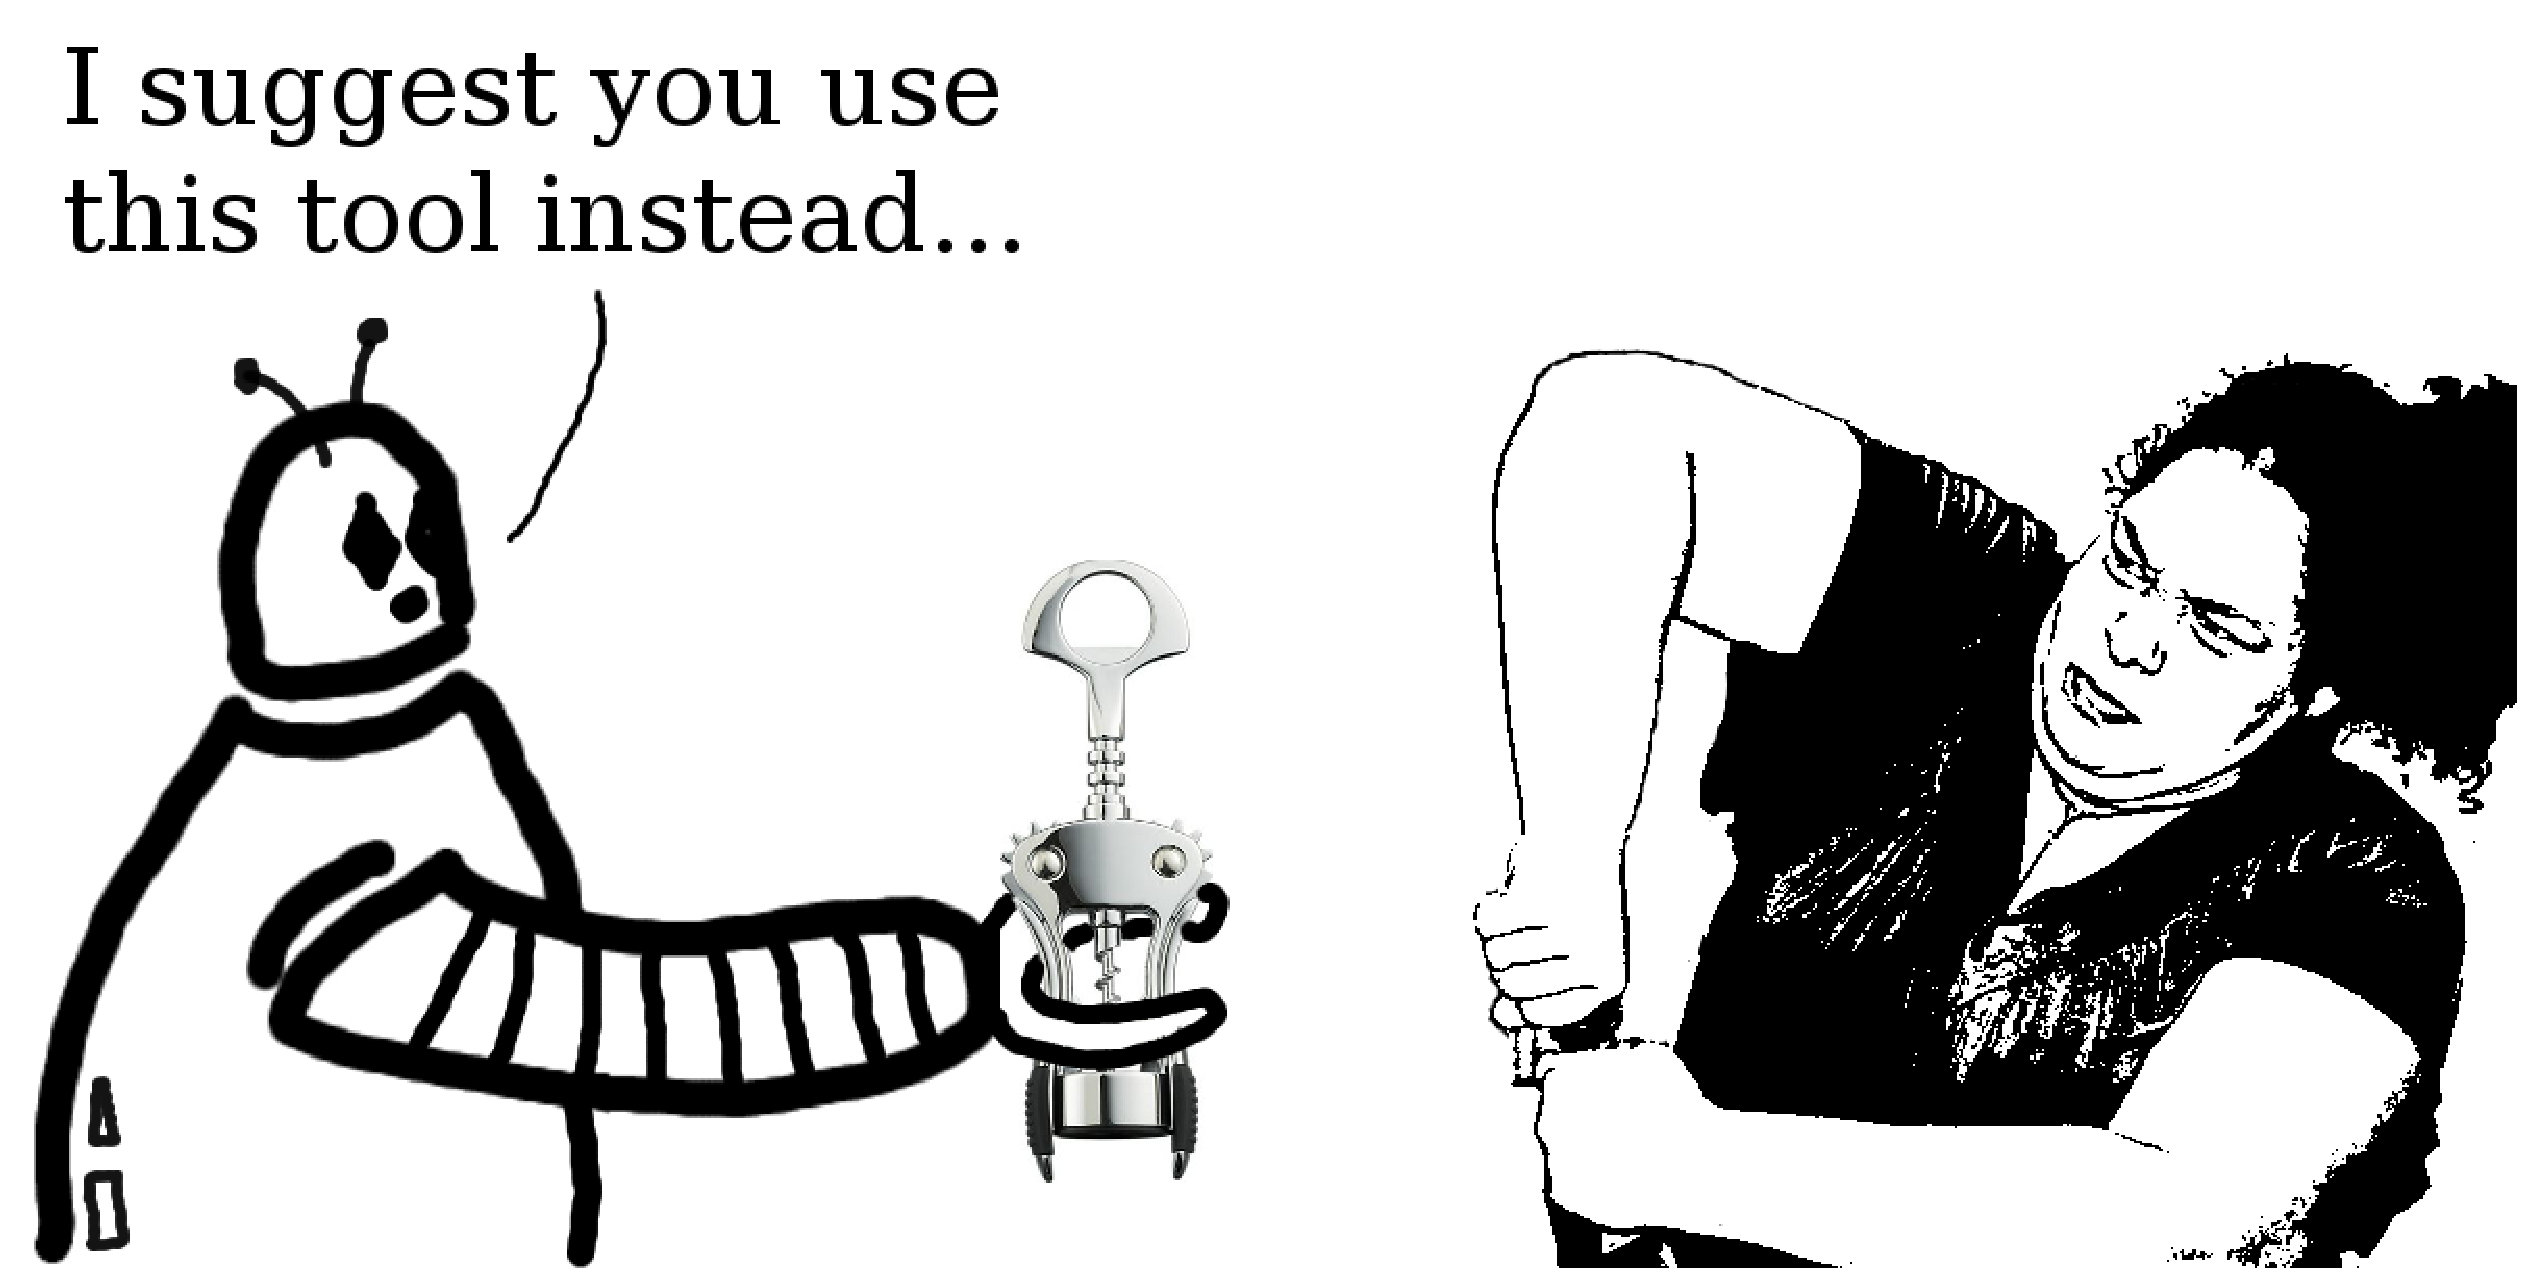
\includegraphics[width=0.9\textwidth]{robot_helper}
\caption[Proof of concept of a robot recognizing a human struggling while opening a bottle: the robot intervenes, providing help.]{Proof of concept of a robot~(left) recognizing a human struggling while opening a bottle~(right): the robot intervenes, providing help.
Picture elaborated from~\url{http://flic.kr/p/b8bbYZ} with permission from the original owner.}
\label{fig:robot_helper}
\end{figure}

A key motivation for using the above-mentioned sources of information~(object affordances, words, gestures) in robot algorithms, is to support \emph{activity recognition} of human agents.
For example, this is useful for revising the belief that a certain action occurred, given the observed effects of the human action onto physical objects (correction of action estimation).
In addition, a robot can anticipate the effects when the action has only been partially observed (early action recognition).
Equipping robots with these prediction capabilities allows them to anticipate effects before action completion, thus enabling interactions between human and robot to be uninterrupted and natural.

In turn, action recognition and prediction abilities serve:
(i)~to predict what is going to happen,
(ii)~to understand the \emph{motivation} beyond the others' action (mental simulation), and
(iii)~to provide feedback or commentary by an automated (possibly robotic) system.
Fig.~\ref{fig:robot_helper} sketches an example of these uses.
Inherent in this motivation is the leap from an ego-centric phase to a social one, permitting agents to reason about the actions of others, and to describe them verbally.
In this chapter, we illustrate our implementation of this process.

\section{Related Work}
\label{sec:gestures:related}

This section describes works that are related to the scope of this chapter, that is, the combination of object affordances with communication~(nonverbal and verbal) in cognitive robotic systems.

First, in Sec.~\ref{sec:gestures:related:salvi} we describe the model by Salvi in greater detail than in Ch.~\ref{chap:background}.
That work is the building block that this chapter extends.
Then, in Sec.~\ref{sec:gestures:related:other} we go through other works in the literature that use robot affordances and communication.

\subsection{Affordances and Language}
\label{sec:gestures:related:salvi}

In Sec.~\ref{sec:background:previous_works:aff_language}, we have introduced the \AffWords{} model by Salvi \cite{salvi:2012:smcb}.

Recall that Salvi proposes a joint model to learn robot affordances \emph{together with word meanings}.
It uses a Bayesian probabilistic framework to allow a robot to ground the basic world behavior and verbal descriptions associated to it, as shown in Fig.~\ref{fig:montesano_setup} on p.~\pageref{fig:montesano_setup} and Fig.~\ref{fig:salvi_setup} on p.~\pageref{fig:salvi_setup}.
The data used for learning such a model is obtained from robot manipulation experiments.
Each experiment is associated with a number of alternative verbal descriptions uttered by two human speakers according to a pre-defined grammar, for a total of \num{1270}~recordings.

Note, however, that in~\cite{salvi:2012:smcb} no grammar was used during the learning phase:
the speech recognizer used as a frontend to the spoken descriptions is based on a loop of words with no grammar, and the \AffWords{} model is based on a bag-of-words assumption, where only the presence or absence of each word in the description is considered.

The data in Salvi's work is acquired from a robot's \emph{ego-centric perspective}, meaning that the robot learns a model by interacting with the environment by self-exploration (see also Sec.~\ref{sec:motivation:devrob} and Sec.~\ref{sec:platform:scenario}), and then it reasons about its own actions.

\begin{figure}
  \tikzstyle{dashedgroup06} = [rectangle, draw, inner sep=0.6cm, dashed, rounded corners, black]
    \centering
    \begin{tikzpicture}
      % single nodes
      \node[affnode] (g1) {$g_1$};
      \node[affnode, right of=g1] (g2) {$g_2$};
      \node[right of=g2] (gdots) {$\dots$};
      \node[group, fit=(g1) (g2) (gdots),label=above:Gesture Features] (gestures) {};
      \node[affnode, below of=gestures] (actions) [below=1cm] {Actions};
      \node[affnode, right of=actions] (f1) [right=1.6cm] {$f_1$};
      \node[affnode, right of=f1] (f2) {$f_2$};
      \node[right of=f2] (fdots) {$\dots$};
      \node[affnode, below of=f1] (e2) [below=0.7cm] {$e_2$};
      \node[affnode, left of=e2] (e1) {$e_1$};
      \node[right of=e2] (edots) {$\dots$};
      \node[wordnode, below of=e1] (w1)  [below=0.7cm] {$w_1$};
      \node[wordnode, right of=w1] (w2) {$w_2$};
      \node[right of=w2] (wdots) {$\dots$};
      % groups
      \node[group, fit=(f1) (f2) (fdots),label=above:Object Features] (features) {};
      \node[group, fit=(e1) (e2) (edots),label=above:Effects] (effects) {};
      \node[group, fit=(w1) (w2) (wdots),label=above:Words] (words) {};
      \node[dashedgroup06, fit=(actions) (features) (effects) (words),label={[shift={(0:2.2)}]above:\AffWords{} model}]{};
      % arrows
      \draw[affarrow] (actions) -- ([xshift=-30pt]effects.north);
      \draw[affarrow] (actions) to [out=260,in=150] (words.west);
      \draw[affarrow] (features) -- ([xshift=20pt]effects.north);
      \draw[affarrow] ([xshift=20pt]features.south) to [out=280,in=30] (words.east);
      \draw[affarrow] ([xshift=30pt]effects.south) -- ([xshift=30pt]words.north);
      % extra
      \draw[affarrow] (actions) -- (gestures);
      \node[dashedgroup06, fit=(actions) (gestures),label=above:Gesture/Action recognition]{};
    \end{tikzpicture}
  \caption[Abstract representation of the probabilistic dependencies in our model which integrates affordances, gestures and language.]{Abstract representation of the probabilistic dependencies in our model which integrates affordances, gestures and language.
  See also Table~\ref{tab:salvi:bnsymb}.}
    \label{fig:gestures:full_model}
\end{figure}

\begin{table}
    \centering
    \caption[Symbolic variables of the \AffWords{} \acl{BN}.]{Symbolic variables of the \AffWords{} \acl{BN} (from~\cite{salvi:2012:smcb}), with the corresponding discrete values obtained from clustering during robot exploration of the environment.
    We call \emph{word variables} the booleans of the last row, whereas we call \emph{affordance variables} all the other symbols.
    See also Fig.~\ref{fig:gestures:full_model}.}
    \label{tab:salvi:bnsymb}
    \begin{tabular}{cp{3.7cm}l}
    \toprule
    symbol & name: description     & values \\
    \midrule
    $a$ & Action: motor action          & grasp, tap, touch \\
    \midrule
    $f_1$ & Color: object color   & blue, yellow, green1, green2 \\
    $f_2$ & Size: object size     & small, medium, big \\
    $f_3$ & Shape: object shape    & sphere, box \\
    \midrule
    $e_1$ & ObjVel: object velocity & slow, medium, fast \\
    $e_2$ & HandVel: robot hand velocity & slow, fast \\
    $e_3$ & ObjHandVel: relative \objecthand{} velocity & slow, medium, fast \\
    $e_4$ & Contact: object hand contact & short, long \\
    \midrule
    $w_1$--$w_{49}$ & presence of each word in the verbal description & true, false \\
    \bottomrule
    \end{tabular}
\end{table}

In this \AffWords{} model, the world behavior is defined by random variables, following the probabilistic machinery introduced in Ch.~\ref{chap:background}.
Table~\ref{tab:salvi:bnsymb} presents a list of variables and their possible values.

All variables are discrete or are discretized from continuous sensory variables through clustering in a preliminary learning phase.

Note that the name of the possible values have been assigned by the researchers arbitrarily to the clusters, for the sake of making the results more human-interpretable.
However, the robot has no prior knowledge about the meaning of these clusters nor about their order, in case they correspond to ordered quantities.

The variables can be divided according to their use: affordance variables and word variables.
Affordance variables are actions variables $A = \{a\}$, object feature variables $F=\{f_1, f_2, \dots\}$, and effect variables $E=\{e_1, e_2, \dots\}$.
Word variables are $W = \{w_1, w_2, \dots\}$.

To simplify the notation, let us call
\begin{align*}
X &= \{A, F, E, W\} \\
  &= \{a, f_1, f_2, \dots, e_1, e_2, \dots, w_1, w_2, \dots\}
\end{align*}
the set of affordance and word variables.
Consequently, the relationships between words and concepts are expressed by the joint probability distribution~$p(X) = p(A, F, E, W)$ of actions, object features, effects, and words in the spoken utterance.

This joint probability distribution,
illustrated by the dashed box labeled \AffWords{} model of Fig.~\ref{fig:gestures:full_model},
is estimated by the robot in an ego-centric way through interaction with the environment.
The dependency structure and the model parameters are estimated by the robot in an ego-centric way through interaction with the environment.
As a consequence, \emph{during learning, the robot knows \apriori{} what action it is performing with certainty, and the variable~$A$ assumes a deterministic value}.
During inference, the probability distribution of the variable~$A$ can be inferred from evidence on the other variables.
For example, if the robot is asked to make a spherical object roll, it will be able to select the action tap as most likely to obtain the desired effect, based on previous experience.

There is no one-to-one correspondence between affordance nodes and words in~\cite{salvi:2012:smcb}.
Each word is connected with many affordance nodes, that constitute the word's significant (for example, the word ``ball'' is not only connected to the shape object feature, but also to action and effect).

The lack of correspondence between affordance nodes and words was partly emerging from the natural variability that is inherent in the way humans describe situations in spoken words.
It was also a design choice, because in that work the authors wanted to prove that the model was not merely able to recover simple \wordmeaning{} associations, but was able to cope with more natural spoken utterances.
Consequently, in the spoken descriptions:
(i)~there are many synonyms for the same concept: for instance, cubic objects are called ``box'', ``square'' or ``cube''. Also, actions and effects are described using different tenses (``is grasping'', ``grasped'', ``has (just) grasped'');
(ii)~different affordance variable values may have the same associated verbal description, e.g., two color clusters corresponding to different shades of green are both referred to as ``green'';
(iii)~finally, many affordance variable values have no direct description: for example, the object velocity and \objecthand{} velocity~(slow, medium, fast), or the \objecthand{} contact~(short, long) are never described directly, and need to be inferred from the situation.

The \AffWords{} model does not account for the concepts of parts of speech, verb tenses or \emph{temporal aspects} explicitly.
For example, the words ``is'', ``grasping'', ``has'', ``grasped'', ``just'', and so on, are initially completely equivalent to the model, which has no prior information about what verbs, adjectives or nouns are, nor about similarity between words.
It is only through the association with the other robot observations that the model realizes that ``grasping'' has the same meaning as ``grasped''\footnote{The model of~\cite{salvi:2012:smcb} has no concept of past, present and future, and cannot distinguish between tenses.}.
The following three phrases, which were used interchangeably in the experiments by \cite{salvi:2012:smcb}, are mapped to exactly the same meaning, after learning:
(i)~``is grasping'',
(ii)~``has grasped'',
(iii)~``grasped''.
Note that the model \emph{per~se} would be fully capable to distinguish between those phrases, provided that they were used in different situations, which however was not the case in the experimental data.

The above assumption
of knowing the action with certainty during learning,
is relaxed in the proposed approach presented further down in this chapter, in Sec.~\ref{sec:gestures:approach}, by extending the model to the observation of external~(human) agents.
In doing this extension, we introduce a \emph{social perspective} where the robot reasons about other agents.

\subsection{Other Works}
\label{sec:gestures:related:other}

A few works have studied the potential coupling between learning robot affordances and \emph{language grounding} (where grounding refers to linking the symbolic nature of language with the sensorimotor experience of a robot).
The union of robot affordances with language grounding gives new skills to cognitive robots, such as:
creation of categorical concepts from multimodal association obtained by grasping and observing objects, while listening to partial verbal descriptions~\cite{nakamura:2009:iros,araki:2012:iros},
learning the association of spoken words with sensorimotor experience~\cite{morse:2016:cogsci}, linking language with sensorimotor representations~\cite{stramandinoli:2016:icdl}, or carrying out complex tasks~(which require \emph{planning} of a sequence of actions) expressed in natural language instructions to a robot.
The planning aspect will be the topic of Ch.~\ref{chap:poeticon++_case_study}.

In other works, both object-directed action recognition in external agents~\cite{koppula:2013:ijrr} and the incorporation of language in \hr{} systems~\cite{harnad:1990,matuszek:2014:aaai} have received ample attention, for example using the concept of \emph{intuitive physics}~\cite{lake:2017:bbs,gao:2018:acl} to be able to predict outcomes from real or simulated interactions with objects.

DeepMind and Google published a method~\cite{santoro:2017:relational_reasoning} to perform relational reasoning on images, i.e., a system that learns to reflect about entities and their mutual relations, with the ability of providing answers to questions such as ``Are there any rubber things that have the same size as the yellow metallic cylinder?''.
That work is very powerful from the point of view of cognitive systems, vision and language.
Our approach is different because
(i)~we focus on \emph{robotic} cognitive systems, including manipulation and the uncertainties inherent to robot vision and control, and
(ii)~we follow the developmental paradigm and the embodiment hypothesis~(see Sec.~\ref{sec:motivation:devrob}), meaning that, leveraging the fact that a human and a humanoid produce actions with similar effects, we relate words with the robot's \emph{sensorimotor} experience, rather than sensory only~(purely images-to-text).

\section{Proposed Approach}
\label{sec:gestures:approach}

In this section, we explain our approach for combining object affordances with communication~(nonverbal and verbal) in cognitive robotic systems.
This combination builds upon the intuition that a robot can use its previously-acquired knowledge of the world~(e.g., motor actions, objects properties, physical effects, verbal descriptions) to those situations where it observes a human agent performing familiar actions in a shared \hr{} scenario.

\subsection{Staged Developmental Process}
\label{sec:gestures:approach:stages}

Our method is a staged developmental process from a self-centered, individualistic learning, to socially aware learning.
This transition happens gradually in subsequent phases.

In the first phase, the system engages in manipulation activities with objects in its environment (following Montesano's approach, as described in Sec.~\ref{sec:background:previous_works:montesano}).
The robot learns object affordances by associating object properties, actions and the corresponding effects.

In a second phase, the robot interacts with a human who uses spoken language to describe the robot's activities (following Salvi's approach, as described in Sec.~\ref{sec:gestures:related:salvi}).
Here, the robot interprets the meaning of the words, grounding them in the \actionperception{} experience acquired so far.
Although this phase can already be considered \emph{social} for the presence of a human \emph{narrator}, it is still self-centered, because the robot is still learning how to interpret its own actions.

\begin{figure*}
  \centering
  \subfloat[][Grasp: moving the hand towards an object vertically, then grasping and lifting it.]{
    \resizebox{\linewidth}{!}{
      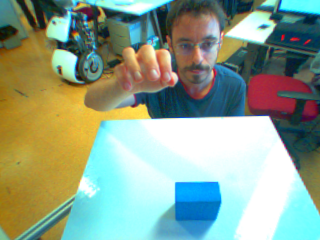
\includegraphics{grasp-00000169}
      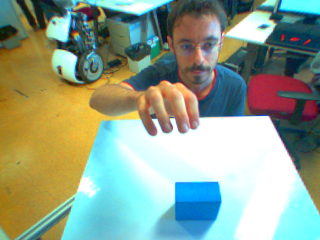
\includegraphics{grasp-00000170}
      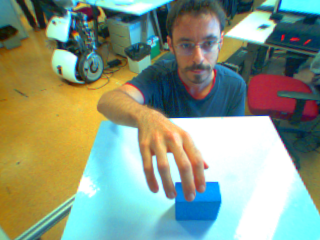
\includegraphics{grasp-00000171}
      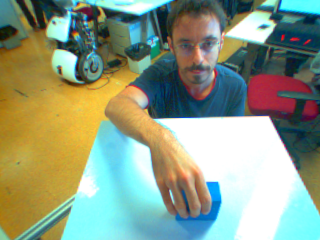
\includegraphics{grasp-00000173}
      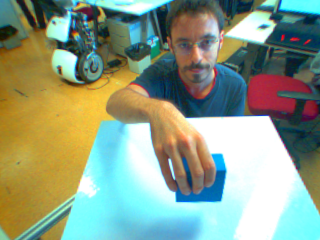
\includegraphics{grasp-00000177}
      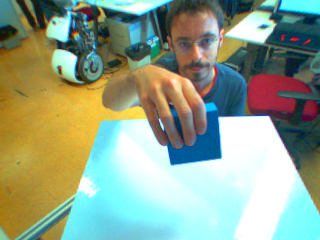
\includegraphics{grasp-00000180}
    } % end resizebox
    \label{fig:gestures:human_action_examples:grasp}
  } % end subfloat

  \subfloat[][Tap: moving the hand towards an object laterally then touching it, causing a motion effect.]{
    \resizebox{\linewidth}{!}{
      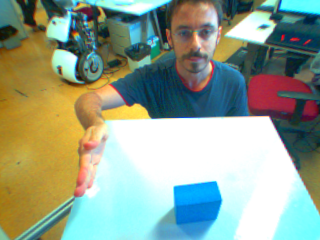
\includegraphics{tap-00000109}
      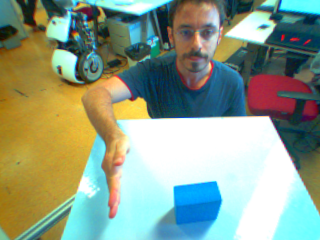
\includegraphics{tap-00000110}
      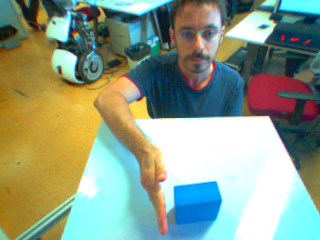
\includegraphics{tap-00000112}
      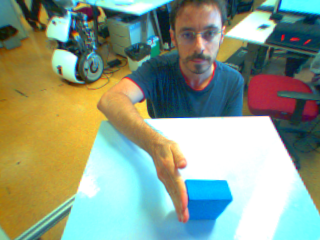
\includegraphics{tap-00000114}
      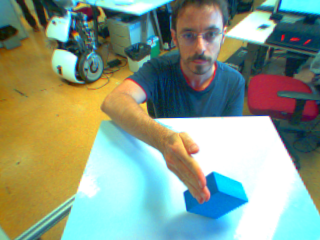
\includegraphics{tap-00000116}
      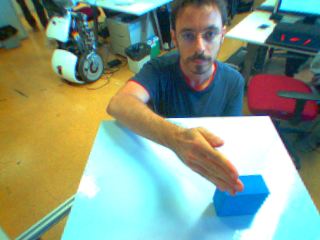
\includegraphics{tap-00000117}
    } % end resizebox
    \label{fig:gestures:human_action_examples:tap}
  } % end subfloat

  \subfloat[][Touch: moving the hand towards an object vertically, touching it~(without grasping), then retracting the hand.]{
    \resizebox{\linewidth}{!}{
      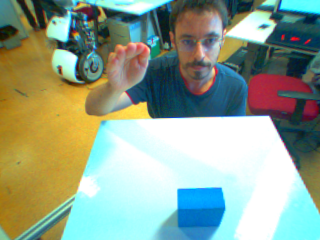
\includegraphics{touch-00000196}
      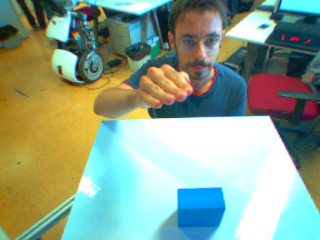
\includegraphics{touch-00000197}
      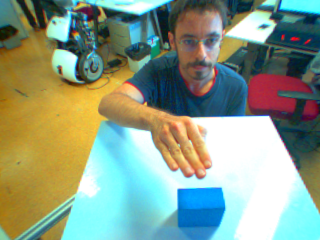
\includegraphics{touch-00000198}
      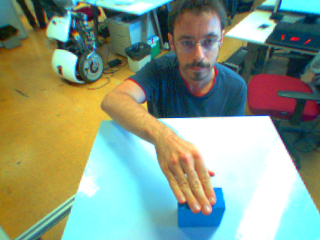
\includegraphics{touch-00000200}
      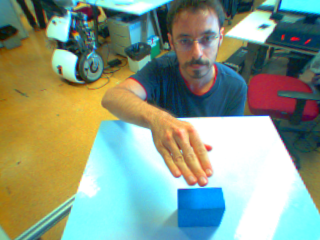
\includegraphics{touch-00000202}
      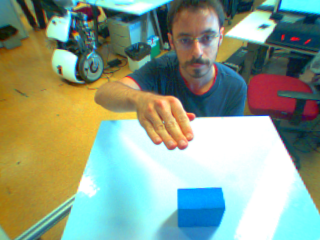
\includegraphics{touch-00000203}
    } % end resizebox
    \label{fig:gestures:human_action_examples:touch}
  } % end subfloat
  \caption{Examples of human manipulative actions from the point of view of the robot.}
  \label{fig:gestures:human_action_examples}
\end{figure*}

In the last phase, which is our contribution, the system turns to observing human actions of a similar nature as the ones explored in the first phases.
We consider three \emph{manipulative gestures}, displayed in Fig.~\ref{fig:gestures:human_action_examples}, corresponding to physical actions performed by an agent onto objects on a table, in a similar fashion as in Sec.~\ref{sec:platform:scenario}.
The robot reuses the experience acquired in the first phases to interpret the new observations between its own actions and the actions performed by the human.
In this phase, human movements are interpreted using the experience acquired so far, and they are incorporated into the model using a gesture recognizer\footref{footnote:link_to_appendix_gest_rec}.

\subsection{Combining Affordances and Communication}
\label{sec:gestures:approach:affgest}

Starting from the \AffWords{} computational model by Salvi \cite{salvi:2012:smcb},
we propose a way to fuse two sources of information~(about the self and about others) in a fully probabilistic manner.
This addition allows to perform fine-grained types of inferences and reasoning, by doing predictions over affordances and words when observing another agent with uncertainty.

In extending Salvi's model, we relax the assumption (described in Sec.~\ref{sec:gestures:related:salvi}) that the action is known during the learning phase.
That assumption is acceptable when the robot learns through self-exploration and interaction with the environment, but must be relaxed if the robot needs to generalize the acquired knowledge through the observation of another~(human) agent.
We estimate the action performed by a human user during a \hr{} collaborative task, by employing a human gesture recognition algorithm\footref{footnote:link_to_appendix_gest_rec}.
This provides two advantages.
First, we can infer the executed action during training.
Second, at testing time we can merge the action information obtained from gesture recognition with the information about affordances.

To permit the transfer from robot self-centered knowledge to human knowledge to work, we assume that the \emph{same actions}, performed on objects with the \emph{same properties}, cause the \emph{same effects} and are described by the \emph{same words}.
In other terms, all of the variables under consideration, listed in Tab.~\ref{tab:salvi:bnsymb}, are the link between robot and human.

In our formulation and in our implementation, we will hinge on the existence of the discrete action variable, the value of which is known to the robot in the ego-centric phase of learning, but must be inferred when observing human actions.

The \emph{gesture recognition model} (that will be fully detailed in Appendix~\ref{chap:gesture_recognition})
is based on a statistical algorithm called \ac{HMM}: therefore, we denote the probabilities obtained by the gesture recognizer as~$\phmm(\cdot)$.
The input of this model is a sequence of~$T$ gesture feature vectors (the sequence going from image frame~$1$ to image frame~$T$), which we define as~$G_1^T$.
Thus, $\phmm(A \given G_1^T)$ denotes the probability distribution over the actions recognized by this model, given gesture features from~$1$ to~$T$.
For example, for a certain input we can obtain that $\phmm(A \given G_1^T)$ corresponds to the following action probabilities summing up to one: grasp~$0.8$, tap~$0.15$, touch~$0.05$.

We define the \AffWords{} model as $\pbn(A, F, E, W)$.
Our goal is to combine the information from $\pbn(A, F, E, W)$ and $\phmm(A \given G_1^T)$ into a single probabilistic model $\pcomb(A, F, E, W \given G_1^T)$, that is, the joint probability of all the affordance and word variables, given that we observe a certain action performed by the human.

The two models can be combined by having the gesture recognizer (Gesture \acp{HMM}) provide a posterior distribution to the \ac{BN}.
The posterior distribution represents a probabilistic or soft decision~\cite{pan:2006:ictai}, as opposed to a deterministic hard decision (which would consider only the top result with full confidence, and would be in fact a less general case, that we described in \cite{saponaro:2017:glu}).

Recall from Sec.~\ref{sec:gestures:related:salvi} that we call $X = \{A, F, E, W\}$ the set of affordance and word variables~$\{a, f_1, f_2, \dots, e_1, e_2, \dots, w_1, w_2, \dots\}$.
During inference, we have a (possibly empty) set of observed variables~$\xobs \subseteq X$, and a set of variables $\xinf \subseteq X$ on which we wish to perform the inference.
In order for the inference to be non-trivial, it must be~$\xobs \cap \xinf = \varnothing$, that is, we should not observe any inference variable.
According to the \ac{BN} alone, without the gesture recognizer, the inference will compute the probability distribution of the inference variables~$\xinf$ given the observed variables~$\xobs$ by marginalizing (see p.~\pageref{para:marginalization}) over all the other latent variables $\xlat = X \setminus (\xobs \cup \xinf)$, where~$\setminus$~is the set difference operation:
\begin{equation*}
 \pbn(\xinf \given \xobs) = \sum_{\xlat} \pbn(\xinf, \xlat \given \xobs).
\end{equation*}

If we want to combine the evidence brought by the \ac{BN} with the evidence brought by the gesture recognizer, there are two cases that can occur:
\begin{enumerate}
\item the variable action is included among the inference variables: $A \in \xinf$, or

\item the variable action is not included among the inference variables: $A \in \xlat$.
\end{enumerate}

Here, we are excluding the case where we observe the action directly~($A \in \xobs$) for two reasons.
First, this would correspond to the robot performing the action by itself, whereas we are interested in interpreting other people's actions, which is a necessary skill to engage in social collaboration with humans.
Second, this would make the evidence on the gesture features~$G_1^T$ irrelevant, because in the model of Fig.~\ref{fig:gestures:full_model}, there is a tail-to-tail connection~(see p.~\pageref{tail_to_tail}) from~$G_1^T$ to the rest of the variables through the action variable, which means that, given the action, all dependencies to the gesture features are dropped.

The two cases 1.,~2. enumerated above can be addressed separately when we do inference.
In the first case, we call~$\xinf^\prime$ the set of inference variables excluding the action~$A$, that is, $\xinf = \{\xinf^\prime, A\}$.
We can write:
\begin{align} \label{eq:pcomb_inf_includes_action}
  & \pcomb(\xinf \given  \xobs, G_1^T) = \pcomb(A, \xinf^\prime \given  \xobs, G_1^T)= \nonumber \\
  &= \sum_{\xlat} \pcomb(A, \xinf^\prime, \xlat \given \xobs, G_1^T)= \nonumber\\
  &= \sum_{\xlat} \left[\pbn(A, \xinf^\prime, \xlat \given \xobs, G_1^T)\right. \nonumber \\[-4mm]
    & \mspace{80mu} \left.\phmm(A, \xinf^\prime, \xlat \given \xobs, G_1^T)\right]= \nonumber \\
  &= \left[\sum_{\xlat} \pbn(A, \xinf^\prime, \xlat \given \xobs)\right] \phmm(A \given G_1^T)= \nonumber \\
  &= \pbn(\xinf \given \xobs) \phmm(A \given G_1^T).
\end{align}
This means that we can evaluate the two models independently, then multiply the distribution that we obtain from the \ac{BN}~(over all the possible value of the inference variables) by the gesture posterior for the corresponding value of the action.

In the second case, where the action is among the latent variables, we define, similarly, $\xlat = \{A, \xlat^\prime\}$, and we have:
\begin{align} \label{eq:pcomb_inf_excludes_action}
  & \pcomb(\xinf \given \xobs, G_1^T) = \nonumber \\
  &= \sum_{\{A,\xlat^\prime\}} \pcomb(\xinf, A, \xlat^\prime \given \xobs, G_1^T)= \nonumber \\
  &= \sum_{\{A,\xlat^\prime\}} \left[\pbn(\xinf, A, \xlat^\prime \given \xobs, G_1^T)\right. \nonumber \\[-4mm]
    & \mspace{100mu} \left.\phmm(\xinf, A, \xlat^\prime \given \xobs, G_1^T)\right]= \nonumber \\[2mm]
  &= \sum_{\{A,\xlat^\prime\}} \left[\pbn(\xinf, A, \xlat^\prime \given \xobs) \phmm(A \given G_1^T)\right]= \nonumber \\
  &= \sum_{A}\left[\phmm(A \given G_1^T)\sum_{\xlat^\prime} \pbn(\xinf, A, \xlat^\prime \given \xobs)\right]= \nonumber \\
  &= \sum_{A}\left[\phmm(A \given G_1^T) \pbn(\xinf, A \given \xobs)\right].
\end{align}
This time, we first need to use the \ac{BN} to do inference on the variables~$\xinf$ and~$A$, and then we marginalize out (see p.~\pageref{para:marginalization}) the action variable~$A$ after having multiplied the probabilities by the gesture posterior.

\subsection{Verbal Descriptions}
\label{sec:gestures:approach:verbal}

In this section, we describe the \emph{verbal language description} capabilities of the combined model described in Sec.~\ref{sec:gestures:approach:affgest}.
These capabilities are made possible by reasoning on the co-occurring verbal descrition of the experiments, linking affordance variables to word variables.

Verbal descriptions allow the robot to:
\begin{itemize}
\item use language in order to determine the mapping between human and own actions, and learn the corresponding perceptual models;

\item use the affordance variables to infer the above mapping even in the absence of verbal descriptions;

\item once the perceptual models for human actions are acquired, use the combined model (\ac{BN} and gestures) to do inference on any variable given some evidence.
\end{itemize}

Such a system makes a robot able to describe the actions of human agents with human language, given some input evidence about the words being uttered and about the visual signals that are detected in the scene.

We use the following notation in order to distinguish between the values of the affordance nodes~(all but the last row in Table~\ref{tab:salvi:bnsymb}) and the words~(last row in the table).
Words and sentences are always enclosed in quotation marks.
For example, ``sphere'' refers to the spoken word, whereas sphere refers to the value of the Shape variable corresponding to the specific cluster.
Similarly, ``grasp'' corresponds to a spoken word, whereas grasp correponds to a value of the action variable.

In Sec.~\ref{sec:gestures:approach:verbal:grammar} we specify the grammar, then in Sec.~\ref{sec:gestures:approach:verbal:descriptions} we outline how we generate and score the verbal descriptions generated from it.

\subsubsection{Grammar Definition}
\label{sec:gestures:approach:verbal:grammar}

The model described above defines a probability distribution over words, given evidence from the scene.
Therefore, it can be used to inspect the understanding by the robot of the current situation.
However, interpreting those probability distributions can be hard.
For this reason, we have augmented the model with a \ac{CFG}\footnote{A \ac{CFG} is a set of recursive rewriting rules~(also called productions) used to generate patterns of strings~\cite{sipser:2012:introtc3}. \label{footnote:cfg}}
that allows us to generate human-readable descriptions from the evidence encoded by the model.

Here, we provide the \emph{grammar definition}.

As a note, recall from Sec.~\ref{sec:gestures:related:salvi} that in~\cite{salvi:2012:smcb}, therefore also in this chapter, no grammar was used during learning:
the model is based on a bag-of-words assumption, where only the presence or absence of each word in the description is considered~(see Sec.~\ref{sec:gestures:approach:verbal:descriptions}).
In other words, the \ac{CFG} will be useful \emph{for interpreting} the results that involve semantic language properties in a human-readable manner (see Sec.~\ref{sec:gestures:results:verbal}), but those results come from our developmental model, not from the grammar itself.

The pre-defined \acl{CFG} uses the following notation.
The symbol \texttt{.|.} represents alternative items, while the symbol \texttt{[.]} optional items.
Non-terminal symbols are given between \texttt{<.>}, while words~(terminal symbols) are given in plain text and font: thus, the full set of words is given by all the plain text words below.

\begin{grammar}
  <sentence> ::= <agent> <action> <object> <conjunction> <object> <effect>

  <agent> ::= the robot | he | baltazar

  <action> ::= <touch> | <poke> | <tap> | <push> | <grasp> | <pick>

  <touch> ::= touches | [has] [just] touched | is touching

  <poke> ::= pokes | [has] [just] poked | is poking

  <tap> ::= taps | [has] [just] tapped | is tapping

  <push> ::= pushes | [has] [just] pushed | is pushing

  <grasp> ::= grasps | [has] [just] grasped | is grasping

  <pick> ::= picks | [has] [just] picked | is picking

  <object> ::= the [<size>] [<color>] <shape>

  <size> ::= big | small

  <color> ::= green | yellow | blue

  <shape> ::= sphere | ball | cube | box | square

  <conjunction> ::= and | but

  <effect> ::= <inertmove> | <slideroll> | <fallrise>

  <inertmove> ::= is inert | is still | moves | is moving

  <slideroll> ::= slides | is sliding | rolls | is rolling

  <fallrise> ::= rises | is rising | falls | is falling
\end{grammar}

\subsubsection{Generation and Scoring}
\label{sec:gestures:approach:verbal:descriptions}

In order to illustrate the language capabilities of the model, rather than displaying the probability distribution of the words inferred by the model, we use the \ac{CFG} described in Sec.~\ref{sec:gestures:approach:verbal:grammar} to generate written descriptions of the robot observations, on the basis of those probabilities.

With our approach, by merging the \AffWords{} model and the gesture recognition model, we allow the robot to \emph{reinterpret} the concepts that it has learned in the self-centered phase, but we do not add any new words to the model.
Consequently, the descriptions that the model generates when observing humans use the same words to describe the agent (see also Sec.~\ref{sec:gestures:results:verbal}).

The textual descriptions are generated as follows.
Given some evidence~$\xobs$ that we provide to the model (not including any $W$ variables) and some human observation features~$G_1^t$ extracted from frames~$1$ to~$t$, we extract the generated word probabilities
$p(w_i \given \xobs, G_1^t)$.
We generate~$N$ sentences randomly from the \ac{CFG} using the \texttt{HSGen} tool from HTK~\cite{young:htkbook}.
Then, the sentences are re-scored according to the log-likelihood of each word in the sentence, normalized by the length of the sentence:
\begin{equation} \label{eq:sentence_score}
  \text{score}(s_j \given \xobs, G_1^t) = \frac{1}{L_j} \sum_{k=1}^{L_j} \log p(w_{jk} \given \xobs, G_1^t),
\end{equation}
where~$s_j$ is the~$j$th sentence,~$L_j$ is the number of words in the sentence~$s_j$, and~$w_{jk}$ is the~$k$th word in the sentence~$s_j$.
Finally, an $N$-best list of possible descriptions is produced by sorting the scores.

\section{Experimental Results}
\label{sec:gestures:results}

In this section, we provide experimental results obtained with our combined model of affordances and communication.
First, in Sec.~\ref{sec:gestures:results:affgest} we focus on the results made possible by incorporating gestures into the \AffWords{} model by Salvi, permitting the social leap towards the observation of other agents.
Then, in Sec.~\ref{sec:gestures:results:verbal} we report the verbal descriptions results in the form of human-interpretable sentences.

\subsection{Combining Affordances and Communication}
\label{sec:gestures:results:affgest}

Because our combined model is based on \aclp{BN} (see Sec.~\ref{sec:background:theory:graphical_models}), it can make inferences over any set of its variables~$\xinf$, given any other set of observed variables~$\xobs$.

In particular, the model can do reasoning on the elements that constitute our computational concept of affordances.
Referring to Fig.~\ref{fig:gestures:full_model}, these are action, object features, and effect elements, as well as words.
We present the following types of results:
\begin{itemize}
  \item inferences over affordance variables~(i.e., over all the entries of Table~\ref{tab:salvi:bnsymb} except the last row therein) in Sec.~\ref{sec:gestures:results:affgest:inference_actions}, \ref{sec:gestures:results:affgest:inference_effects}, \ref{sec:gestures:results:anticipation_effects};

  \item predictions of word probabilities~(i.e., predictions of the last row entry of Table~\ref{tab:salvi:bnsymb}) in Sec.~\ref{sec:gestures:results:affgest:prediction_words};

  \item verbal descriptions generated from the word probabilities of the previous point, according to a \ac{CFG} (see footnote~\footref{footnote:cfg} on p.~\pageref{footnote:cfg}).
  These descriptions are useful for clear human interpretation.
  They serve as a way to observe the emergence (from the model) of certain language phenomena: Sec.~\ref{sec:gestures:results:verbal:descriptions_and_synonyms}, \ref{sec:gestures:results:verbal:conjunction}, \ref{sec:gestures:results:verbal:description_objects}.
\end{itemize}

\subsubsection{Inference over Action}
\label{sec:gestures:results:affgest:inference_actions}

\begin{figure}
\centering
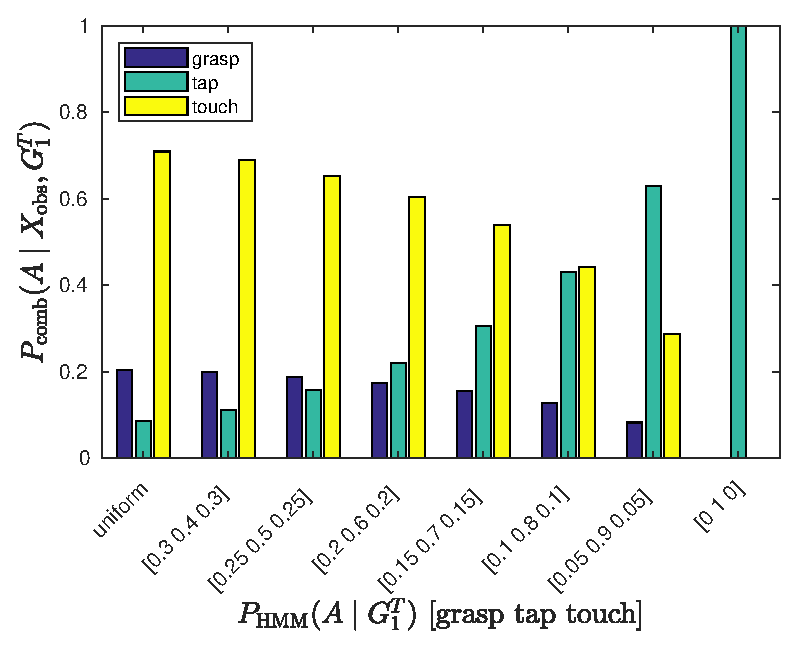
\includegraphics[width=0.9\columnwidth]{impact_of_evidence_on_Action.eps}
\caption{Affordances and gestures combined model: inference over action given the evidence $\xobs =\{\text{Size}=\text{small}, \text{Shape}=\text{sphere}, \text{ObjVel}=\text{slow}\}$, combined with different probabilistic soft evidence about the action.}
\label{fig:impact_of_evidence_on_Action}
\end{figure}

In this experiment, we test the ability of our approach to recognize actions.
Both the \AffWords{} model and the gesture recognizer can each perform inference of the action variable individually: the former by using the variables of Tab.~\ref{tab:salvi:bnsymb}, the latter by using human gesture features.
We show how our combined model performs the inference over action in a joint way.
This includes dealing with information with different degrees of confidence, or conflicting information.

Let us consider the evidence
$\xobs = \{$ Size=small, Shape=sphere, ObjVel=slow~$\}$.
This corresponds to an experiment that involves a small ball which, after the manipulative action, exhibits a low velocity.
Fig.~\ref{fig:impact_of_evidence_on_Action} displays the inference over the action variable by our model.

Based on the evidence, the affordance model alone gives the highest probability $\pbn(A \given \xobs)$ to the action \emph{touch}, which usually (in training) does not result in any movement of the object.
However, in this particular situation, let us further assume that the action performed by the human was an (unsuccessful) \emph{tap}, that is, a tap that does not result in any movement for the object.

In the figure, we show the effect of augmenting the inference with information from the gesture recognizer, that is, computing \eqref{eq:pcomb_inf_includes_action} (in the case where the action variable is included among the inference variables).
We analyze the effect of varying the degree of confidence of the gesture classifier.
We start from a uniform posterior $\phmm(A \given G_1^T)$, corresponding to a poor classifier, and gradually increase the probability of the correct action until it reaches~$1$.
In this particular example, in order to win the belief of the affordance model, the gesture recognizer needs to be very confident ($\phmm(A=\text{tap} \given G_1^T) > 0.81$).

\subsubsection{Inference over Effects}
\label{sec:gestures:results:affgest:inference_effects}

\begin{figure*}
\centering
\subfloat[][Predictions with a sphere object.]
{ 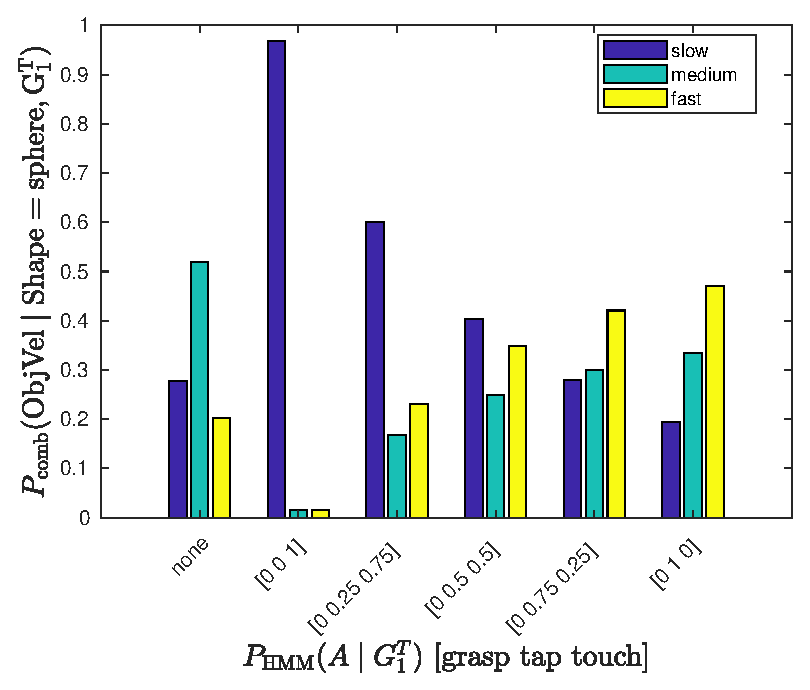
\includegraphics[width=0.45\linewidth]{impact_of_evidence_on_ObjVel_sphere.eps} \label{fig:impact_of_evidence_on_ObjVel_sphere} } \quad
%
\subfloat[][Predictions with a box object.]
{ 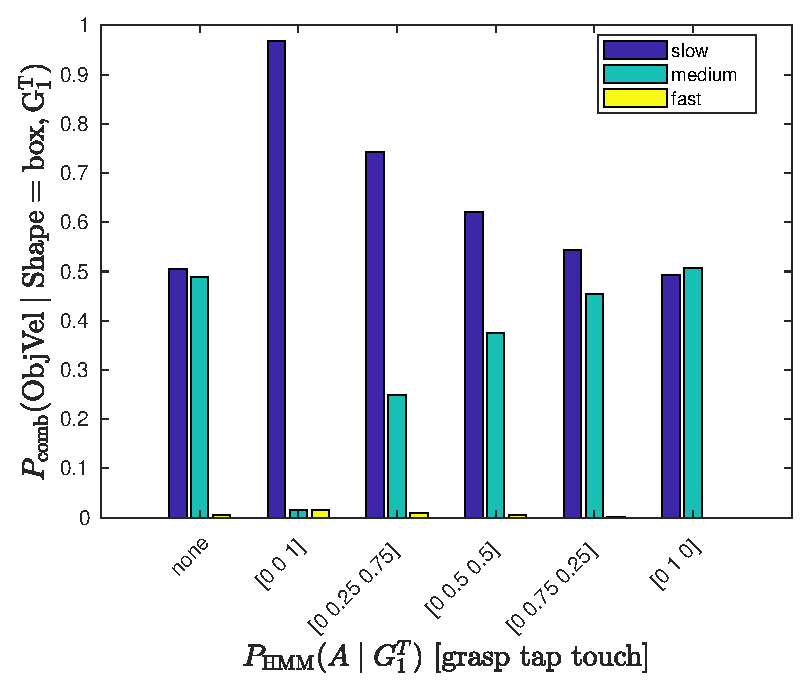
\includegraphics[width=0.45\linewidth]{impact_of_evidence_on_ObjVel_box.eps} \label{fig:impact_of_evidence_on_ObjVel_box} }
\caption{Affordances and gestures combined model: inference over the object velocity effect of different objects, when given probabilistic soft evidence about the action.}
\label{fig:impact_of_evidence_on_ObjVel}
\end{figure*}

We now show how our approach does inference over variables other than the action one.
This corresponds to computing \eqref{eq:pcomb_inf_excludes_action} (in the case where the action variable is not among the inference variables, but it is among the latent variables).

We will run this test by using different degrees of probabilistic confidence about the action, and analyzing the outcome in terms of velocity prediction.
This experiment exposes that \emph{all} the variables of Tab.~\ref{tab:salvi:bnsymb} jointly link robot and human, not only the action variable, for the reasons expressed in Sec.~\ref{sec:gestures:approach:affgest}.

Fig.~\ref{fig:impact_of_evidence_on_ObjVel} shows the considered inference in two cases: when the prior information indicates that the shape is spherical~(see Fig.~\ref{fig:impact_of_evidence_on_ObjVel_sphere}), and when it is cubic~(see Fig.~\ref{fig:impact_of_evidence_on_ObjVel_box}).

The leftmost distribution in both figures shows the prediction of object velocity from the \AffWords{} model alone, without any additional information.
When the shape is spherical, the model is not sure about the velocity, whereas if the shape is cubic, the model does not expect high velocities.
If we add clear evidence on the action \emph{touch} from the gesture recognizer, suddenly the combined model predicts slow velocities in both cases, as expected.
However, if the action recognition evidence is gradually changed from \emph{touch} to \emph{tap}, the predictions of the model depend on the shape of the object.
Higher velocities are expected for spherical objects that can roll, compared to cubic objects.

\subsubsection{Prediction of Word Probabilities}
\label{sec:gestures:results:affgest:prediction_words}

\begin{figure}
\centering
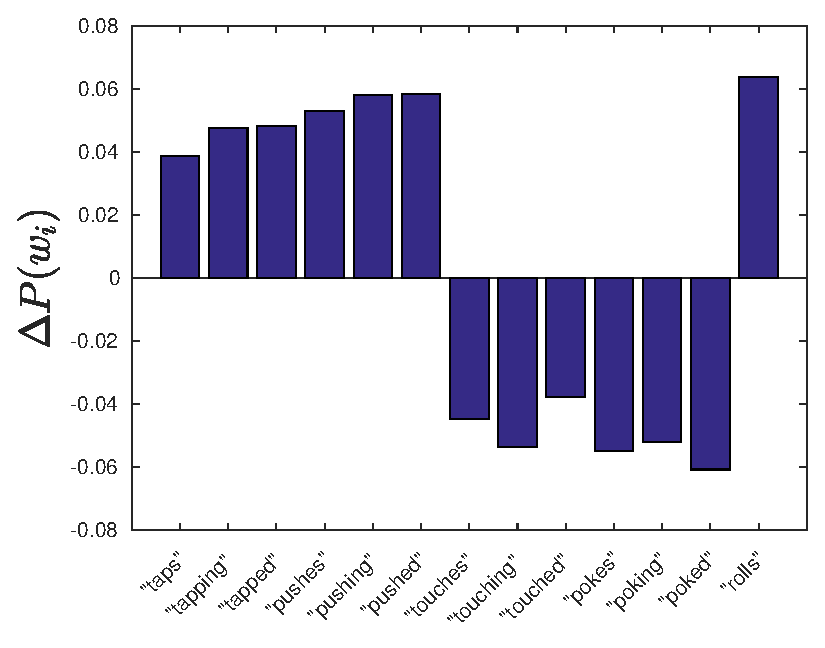
\includegraphics[width=0.9\columnwidth]{tcds-partialfig.eps}
\caption[Affordances and verbal language: variation of word occurrence probabilities.]{Affordances and verbal language: variation of word occurrence probabilities
$\Delta p(w_i) = \pcomb(w_i \given \xobs, \text{Action=tap}) - \pbn(w_i \given \xobs)$, where $\xobs = \{ \text{Size=big, Shape=sphere, ObjVel=fast} \}$.
This variation corresponds to the difference of word probability when we add the tap action evidence~(obtained from gesture recognition) to the initial evidence about object features and effects. We have omitted words for which no significant variation was observed.}
\label{fig:variation_word_occurrence_prob}
\end{figure}

Our model permits to make predictions over the word variables associated to affordance evidence (see Table~\ref{tab:salvi:bnsymb}, last row).
In Fig.~\ref{fig:variation_word_occurrence_prob} we show the variation in word occurrence probabilities between two cases:
\begin{enumerate}
\item when the robot's prior knowledge evidence consists of information about object features and effects only: \{Size=big, Shape=sphere, ObjVel=fast\};

\item when the evidence corresponds to the one of the previous point, with the addition of the \emph{tap} action observed from the gesture recognizer (deterministic hard evidence).
\end{enumerate}

This result is interesting for two reasons.
First, the probabilities of words related to tapping and pushing increase when a tapping action evidence from the gesture recognizer is introduced; conversely, the probabilities of other action words~(touching and poking) decreases.
Second, the probability of the word ``rolling''~(which is an effect of an action onto an object) also increases when the tap action evidence is entered.

\subsubsection{Effect Anticipation}
\label{sec:gestures:results:anticipation_effects}

\begin{figure*}
  \centering
  \subfloat[][Action performed on small sphere. Description: ``the robot pushed the ball and the ball moves''.]{
    \resizebox{0.9\linewidth}{!}{
      \begin{tikzpicture}
        \node (lik) {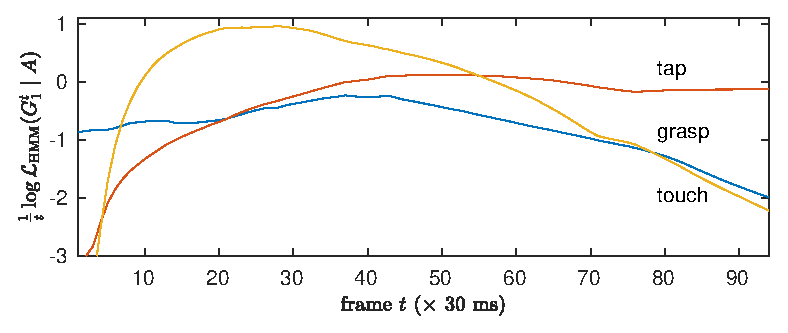
\includegraphics[width=0.6\linewidth]{evolution_of_action_posterior_sphere_log.eps}};
        \node at ([xshift=-90pt,yshift=30pt]lik.north) {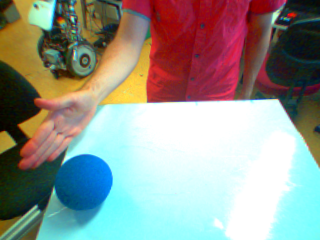
\includegraphics[width=\myWidthTcds\linewidth]{tap-sphere-00000179}};
        \node at ([xshift=+10pt,yshift=30pt]lik.north) {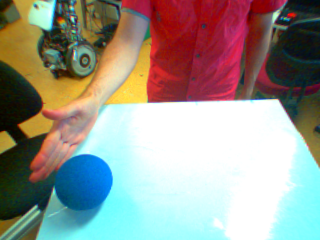
\includegraphics[width=\myWidthTcds\linewidth]{tap-sphere-00000183}};
        \node at ([xshift=+110pt,yshift=30pt]lik.north) {\includegraphics[width=\myWidthTcds\linewidth]{tap-sphere-00000187}};
        \node at ([xshift=100pt,yshift=30pt]lik.east) {\includegraphics[width=0.35\linewidth]{evolution_of_action_posterior_sphere_effect_pred.eps}};
      \end{tikzpicture}
    } % end resizebox
    \label{fig:effect_pred_sphere}
  } % end subfloat

  \subfloat[][Action performed on big box. Description: ``the robot is pushing the big square but the box is inert''.]{
    \resizebox{0.9\linewidth}{!}{
      \begin{tikzpicture}
        \node (lik) {\includegraphics[width=0.6\linewidth]{evolution_of_action_posterior_box_log.eps}};
        \node at ([xshift=-90pt,yshift=30pt]lik.north) {\includegraphics[width=\myWidthTcds\linewidth]{tap-box-00000230}};
        \node at ([xshift=+10pt,yshift=30pt]lik.north) {\includegraphics[width=\myWidthTcds\linewidth]{tap-box-00000250}};
        \node at ([xshift=+110pt,yshift=30pt]lik.north) {\includegraphics[width=\myWidthTcds\linewidth]{tap-box-00000270}};
        \node at ([xshift=100pt,yshift=30pt]lik.east) {\includegraphics[width=0.35\linewidth]{evolution_of_action_posterior_box_effect_pred.eps}};
      \end{tikzpicture}
    } % end resizebox
  \label{fig:effect_pred_box}
  } % end subfloat
  \caption[Affordances and gestures combined model: object velocity effect anticipation before impact.]{Affordances and gestures combined model: object velocity effect anticipation before impact. The evidence from the gesture recognizer~(left) is fed into the \AffWords{} model before the end of the execution. The combined model predicts the effect~(right) and describes it in words~(verbal language).}
  \label{fig:effect_pred}
\end{figure*}

Since the gesture recognition method interprets sequences of human motions, we can test this predictive ability of our combined model when we observe an incomplete action.
Fig.~\ref{fig:effect_pred} shows an example of this where we reason about the expected object velocity caused by a tap action.

In particular, Fig.~\ref{fig:effect_pred_sphere} shows the action performed on a spherical object, whereas Fig.~\ref{fig:effect_pred_box} on a cubic one.
Within each of the two figures, the graphs on the left side show the time evolution of the evidence $\phmm(A \given G_1^t)$ from the gesture recognizer.
In order to make the variations emerge more clearly, instead of the posterior, we show $\frac{1}{t} \log \mathcal{L}_\text{HMM} (G_1^t \given A)$: the log-likelihood normalized by the length of the sequence.

Note how, in both cases, the correct action is recognized by the model given enough evidence, although the observation sequence is not complete.
The right side of the plot shows the prediction of the object velocity, given the incomplete observation of the action and the object properties.
The model correctly predicts that the sphere will probably move but the box is unlikely do so.
Finally, the captions in the figure also show the human-interpretable verbal description~(see Sec.~\ref{sec:gestures:approach:verbal}) generated by feeding the probability distribution of the words estimated by the model, given incomplete evidence, into the \ac{CFG}.

\subsection{Verbal Descriptions}
\label{sec:gestures:results:verbal}

We now present results about the verbal descriptions generated by the model with the \ac{CFG}.
They allow us to observe the emergence of non-trivial language phenomena (they emerge from our developmental model, not from the grammar itself, which is provided only for the purpose of interpreting the probability distributions over the words).

By generating and scoring verbal descriptions about what the robot observes~(see Sec.~\ref{sec:gestures:approach:verbal}), we can provide evidence to the model and interpret the verbal results.

From Sec.~\ref{sec:gestures:approach:verbal:descriptions} recall that, with our method, we do not add new words to the model when we observe the human performing actions.
Rather, the human-readable descriptions that we generate are based on the same words that were present in the self-centered learning phase (see Sec.~\ref{sec:gestures:approach:stages}).
In that phase, the verbal descriptions described the agent of the observed actions as either ``the~robot'', ``he'', or ``Baltazar''~(the name of the robot used in \cite{salvi:2012:smcb}).
Consequently, the \AffWords{} model learned by the robot includes those words as the subject of the action.

\subsubsection{Choice of Synonyms}
\label{sec:gestures:results:verbal:descriptions_and_synonyms}

\begin{table}
    \centering
    \caption{Affordances and verbal language: $10$-best list of sentences generated from the evidence $\xobs = \{ \text{Color=yellow, Size=big, Shape=sphere, ObjVel=fast} \}$.}
    \label{tab:example_generated_sentences}
    \resizebox{\linewidth}{!}{% https://tex.stackexchange.com/a/27105
    \begin{tabular}{ll}
    \toprule
    sentence & score \\
    \midrule
    ``the robot pushed the ball and the ball moves'' & $-0.54322$ \\
    ``the robot tapped the sphere and the sphere moves'' & $-0.5605$ \\
    ``he is pushing the sphere and the sphere moves'' & $-0.57731$ \\
    ``the robot is tapping the yellow ball and the big yellow sphere is moving'' & $-0.57932$ \\
    ``he pushed the yellow ball and the sphere is rolling'' & $-0.58853$ \\
    ``the robot is poking the ball and the sphere is rolling'' & $-0.58998$ \\
    ``he is pushing the ball and the yellow ball moves'' & $-0.59728$ \\
    ``he pushes the sphere and the ball is moving'' & $-0.60528$ \\
    ``he is tapping the yellow ball and the ball is moving'' & $-0.60675$ \\
    ``the robot pokes the sphere and the ball is rolling'' & $-0.60694$ \\
    \bottomrule
    \end{tabular}%
    } % end resizebox
\end{table}

As an example, by providing the evidence $\xobs=$\{Color=yellow, Size=big, Shape=sphere, ObjVel=fast\} to the model, we obtain the sentences reported in Table~\ref{tab:example_generated_sentences}.
The higher the score, the more likely the sentence.

In many of the sentences in the table, we note that
(i)~the correct verb related to the tap action is generated (in the initial evidence, no action information was present, only object features and effects information were), and
(ii)~the object term ``ball'' or synonyms thereof~(e.g., ``sphere'') are used coherently, both in the first part of the sentence describing the action and in the second part describing the effect.

This result shows that different synonyms may be used by the model in the same sentence.
This is a consequence of the random generation of sentences, described in Sec.~\ref{sec:gestures:approach:verbal:descriptions}, and because synonyms are often assigned similar (but not necessarily equal) probabilities by the model, given the same evidence.

\subsubsection{Choice of Conjunction}
\label{sec:gestures:results:verbal:conjunction}

The manipulation experiments that we consider in this chapter have the following structure, similar to the one described in Sec.~\ref{sec:platform:scenario}: an agent~(human or robot) performs a physical action onto an object with certain properties, and this object will show a certain physical effect as a result.
For example, a touch action on an object yields no physical movement, but a tap does~(especially if the object is spherical).
In the language description associated to an experiment, it makes sense to analyze the \emph{conjunction} chosen by the model given specific evidence.
In particular, it would be desirable to separate two kinds of behaviors: one in which the action and effect are coherent~(expected conjunction: ``and''), and the other one in which they are contradictory (``but'').

\newcommand{\evidenceProducingAnd}{$\xobs=$\{ Action=grasp, ObjVel=medium \}}
\newcommand{\evidenceProducingBut}{$\xobs=$\{ Action=grasp, ObjVel=slow \}}

\begin{figure*}
  \centering
  \subfloat[][Evidence: \evidenceProducingAnd.]{
    \begin{tabular}[b]{c}
    \includegraphics[width=0.4\linewidth]{p_conjunctions_and_evidence.eps}\\

    \resizebox{!}{0.1\linewidth}{% https://tex.stackexchange.com/a/27105
      \begin{tabular}{ll}
        \toprule
        sentence & score \\
        \midrule
        ``the robot is picking the sphere \textbf{and} the sphere is moving''  & $-0.59328$ \\
        ``the robot grasps the sphere \textbf{and} the ball is moving''  & $-0.59507$ \\
        ``the robot is picking the sphere \textbf{and} the sphere is rising''  & $-0.60882$ \\
        ``the robot grasped the sphere \textbf{and} the sphere is rising''  & $-0.61842$ \\
        ``the robot picked the ball \textbf{and} the ball is rising''  & $-0.64052$ \\
        ``baltazar grasps the sphere \textbf{and} the sphere is moving''  & $-0.66182$ \\
        ``the robot has grasped the ball \textbf{and} the ball is rising''  & $-0.66398$ \\
        ``the robot picked the ball \textbf{and} the green ball is moving''  & $-0.67134$ \\
        ``baltazar grasped the sphere \textbf{and} the ball is moving''  & $-0.67283$ \\
        ``baltazar is grasping the ball \textbf{and} the sphere is rising''  & $-0.6787$ \\
        \bottomrule
      \end{tabular}%
    } % end resizebox
    \end{tabular}
    \label{tab:conjunction:and}
  } % end subfloat
  \quad
  \subfloat[][Evidence: \evidenceProducingBut.]{
    \begin{tabular}[b]{c}
    \includegraphics[width=0.4\linewidth]{p_conjunctions_but_evidence.eps}\\

    \resizebox{!}{0.1\linewidth}{% https://tex.stackexchange.com/a/27105
      \begin{tabular}{ll}
        \toprule
        sentence & score \\
        \midrule
        ``the robot is picking the cube \textbf{but} the square is still''  & $-0.52575$ \\
        ``the robot is grasping the sphere \textbf{but} the box is inert''  & $-0.55$ \\
        ``the robot is grasping the square \textbf{but} the sphere is still''  & $-0.55388$ \\
        ``the robot grasped the square \textbf{but} the cube is inert''  & $-0.55608$ \\
        ``baltazar is grasping the square \textbf{but} the square is inert''  & $-0.5571$ \\
        ``the robot is grasping the cube \textbf{but} the ball is inert''  & $-0.56011$ \\
        ``the robot picks the box \textbf{but} the square is inert''  & $-0.56397$ \\
        ``baltazar is picking the square \textbf{but} the square is still''  & $-0.56402$ \\
        ``he is grasping the square \textbf{but} the cube is inert''  & $-0.56815$ \\
        ``the robot grasps the square \textbf{but} the sphere is inert''  & $-0.57417$ \\
        \bottomrule
      \end{tabular}%
    } % end resizebox
    \end{tabular}
    \label{tab:conjunction:but}
  } % end subfloat
    \caption[Affordances and verbal language: $10$-best list of sentences generated given two different sets of evidence.]%
    {Affordances and verbal language: $10$-best list of sentences generated given two different sets of evidence.
    In~(a) the model interprets the object movement as indicating a succesful grasp and uses the conjunction ``and''.
    In~(b) the slow movement is interpreted as no movement at all and, therefore, as an unsuccessful grasp: for that reason, the conjunction ``but'' is used.}
    \label{tab:conjunction}
\end{figure*}

Fig.~\ref{tab:conjunction} shows an example of the behavior described above.
We give the same action value \emph{grasp} to the model as evidence, but two different values for the final object velocity.
When the object velocity is medium~(Fig.~\ref{tab:conjunction:and}), the model interprets this as a successful grasp, and it uses the conjunction ``and'' to separate the description of the action from the description of the effect.
When the object velocity is slow~(in the clustering procedure, the velocity was most often zero in those cases), the model predicts that this is an unsuccessful grasp and it uses the conjunction ``but'', instead.

\subsubsection{Description of Object Features}
\label{sec:gestures:results:verbal:description_objects}

\newcommand{\graspBoxGreenOne}{``the robot is grasping the box and the green box is moving''}
\newcommand{\touchBoxGreenOne}{``the robot is poking the green square and the cube is inert''}
\newcommand{\graspSphereGreenTwo}{``the robot picked the ball and the green ball is moving''}
\newcommand{\touchSphereGreenTwo}{``baltazar is poking the green sphere and the sphere is still''}

\newcommand{\evidenceProducingGraspBoxGreenOne}{$\xobs = \{ \text{Action=grasp, Color=green1, Shape=box} \}$}
\newcommand{\evidenceProducingTouchBoxGreenOne}{$\xobs = \{ \text{Action=touch, Color=green1, Shape=box} \}$}
\newcommand{\evidenceProducingGraspSphereGreenTwo}{$\xobs = \{ \text{Action=grasp, Color=green2, Shape=sphere} \}$}
\newcommand{\evidenceProducingTouchSphereGreenTwo}{$\xobs = \{ \text{Action=touch, Color=green2, Shape=sphere} \}$}

\begin{figure}
  \centering
  \subfloat[][\graspBoxGreenOne.]{
    \resizebox{\linewidth}{!}{
      \includegraphics{graspBoxGreen1-00000007}
      \includegraphics{graspBoxGreen1-00000008}
      \includegraphics{graspBoxGreen1-00000009}
      \includegraphics{graspBoxGreen1-00000010}
      \includegraphics{graspBoxGreen1-00000013}
      \includegraphics{graspBoxGreen1-00000016}
    } % end resizebox
    \label{fig:verbal_descriptions:graspBoxGreenOne}
  } % end subfloat

  \subfloat[][\touchBoxGreenOne.]{
    \resizebox{\linewidth}{!}{
      \includegraphics{touchBoxGreen1-00000008}
      \includegraphics{touchBoxGreen1-00000009}
      \includegraphics{touchBoxGreen1-00000010}
      \includegraphics{touchBoxGreen1-00000011}
      \includegraphics{touchBoxGreen1-00000013}
      \includegraphics{touchBoxGreen1-00000015}
    } % end resizebox
    \label{fig:verbal_descriptions:touchBoxGreenOne}
  } % end subfloat

  \subfloat[][\graspSphereGreenTwo.]{
    \resizebox{\linewidth}{!}{
      \includegraphics{graspSphereGreen2-00000007}
      \includegraphics{graspSphereGreen2-00000008}
      \includegraphics{graspSphereGreen2-00000009}
      \includegraphics{graspSphereGreen2-00000011}
      \includegraphics{graspSphereGreen2-00000013}
      \includegraphics{graspSphereGreen2-00000015}
    } % end resizebox
    \label{fig:verbal_descriptions:graspSphereGreenTwo}
  } % end subfloat

  \subfloat[][\touchSphereGreenTwo.]{
    \resizebox{\linewidth}{!}{
      \includegraphics{touchSphereGreen2-00000006}
      \includegraphics{touchSphereGreen2-00000007}
      \includegraphics{touchSphereGreen2-00000008}
      \includegraphics{touchSphereGreen2-00000010}
      \includegraphics{touchSphereGreen2-00000011}
      \includegraphics{touchSphereGreen2-00000012}
    } % end resizebox
    \label{fig:verbal_descriptions:touchSphereGreenTwo}
  } % end subfloat

  \caption{Affordances and verbal language: examples of descriptions generated by the model.}
  \label{fig:verbal_descriptions}
\end{figure}

In Fig.~\ref{fig:verbal_descriptions}, we show examples of verbal descriptions generated by the model given different values of observed evidence:
\begin{itemize}
\item \evidenceProducingGraspBoxGreenOne{} (Fig.~\ref{fig:verbal_descriptions:graspBoxGreenOne});

\item \evidenceProducingTouchBoxGreenOne{} (Fig.~\ref{fig:verbal_descriptions:touchBoxGreenOne});

\item \evidenceProducingGraspSphereGreenTwo{} (Fig.~\ref{fig:verbal_descriptions:graspSphereGreenTwo});

\item \evidenceProducingTouchSphereGreenTwo{} (Fig.~\ref{fig:verbal_descriptions:touchSphereGreenTwo}).
\end{itemize}
Note that the box object in the two first examples has a dark shade of green~(value of Color affordance variable of Table~\ref{tab:salvi:bnsymb} clustered as:~green1), whereas the spherical one in the two last examples has a lighter shade (Color value:~green2).
However, the verbal descriptions reported in Fig.~\ref{fig:verbal_descriptions} all use the adjective ``green''.
This behavior emerges from fact that the robot develops its perceptual symbols (clusters) in an early phase, and only subsequently associates them with the human vocabulary.
We believe that this phenomenon is practical and potentially useful~(i.e., the possibility that a low-level fine-grained robot representation can be abstracted into a high-level language description, which bundles the two shades of green under the same word).

\section{Conclusions and Future Work}
\label{sec:gestures:conclusions}

This chapter has illustrated a computational model that combines object affordances, human gestures and verbal language.
We presented such a combined model, allowing a robot to interpret and describe the actions of external agents, by reusing the knowledge previously acquired in an ego-centric manner.

We have shown that for cognitive robots it is possible, and indeed fruitful, to combine knowledge acquired from interacting with elements of the environment~(affordances) with the probabilistic observation of another agent's actions~(gestures) as well as verbal language elements.
In this sense, our model supports the growing field of \emph{\hr{} collaboration}~\cite{bauer:2008:ijhr,dragan:2015:hri}, whose goal is to enable effective teamwork between humans and robots.

In a developmental setting, the robot learns the link between words and object affordances by exploring its environment.
Then, it classifies the manipulative gestures performed by another agent.
Finally, by fusing the information from the affordances model and a gesture recognizer, the robot can reason over affordances and words when observing the other agent.
This can also be leveraged to do early action recognition~(see Sec.~\ref{sec:gestures:results:anticipation_effects}).

In terms of language, although the complete model only estimates probabilities of single words given the evidence, we showed that feeding these probabilities into a pre-defined grammar produces human-interpretable sentences that correctly describe the situation.
We also highlighted some interesting language-related properties of the combined model, such as:
the choice of relevant words to describe a scene,
the choice of synonyms,
and of congruent/incongruent conjunctions,

Our demonstrations are based on a restricted scenario~(see Sec.~\ref{sec:gestures:related:salvi}), i.e., one human and one robot manipulating simple objects on a shared table, a pre-defined number of motor actions and effects, and a vocabulary of approximately~$50$ words to describe the experiments verbally.
However, one of the main strengths of our study is that it spans different fields such as robot learning, language grounding, and object affordances.
We also work with real robotic data, as opposed to learning images-to-text mappings~(as in many works in computer vision) or using robot simulations~(as in many works in robotics).

In terms of \emph{scalability}, note that our \ac{BN} model can learn both the dependency structure and the parameters of the model from observations.
The method that estimates the dependency structure, in particular, is sensitive to biases in the data.
Consequently, in order to avoid misconceptions, the robot needs to explore any possible situation that may occur.
For example, if the robot only observes blue spheres rolling and the objects with any other shape are never blue, it might infer that it is the color that makes the object roll, rather than its shape.
In order to scale the method to a larger number of concepts, it would be necessary to scale the amount of data considerably, similarly to what is done in many deep learning approaches.
In models of developmental robotics, where this is neither practically feasible, nor desirable, we would need to devise methods that can generalize more efficiently from very few observations.

As future work, it would be useful to investigate how the model can extract syntactic information from the observed data autonomously, thus relaxing the bag-of-words assumption in the current model.
Another line of research would be to study how the model can guide the discovery of new acoustic patterns~(e.g., \cite{falstrom:2017:glu, vanhainen:2014:icassp, vanhainen:2012:interspeech}), and how to incorporate the newly discovered symbols into our \AffWords{} model.
This would release our current assumption of a pre-defined set of words.


%!TEX encoding = UTF-8

\chapter{Tool Use Affordances}
\label{chap:tool}

In this chapter, we present a computational model of affordances capable of dealing with multiple objects (see Fig.~\ref{fig:tool:tools_computational_model}), giving rise to a \emph{tool use} behavior.
This skill is useful to operate in complex manipulation tasks typical of human-like environments.

\begin{figure}[h]
\newcommand{\myscaleaffmodels}{0.6}
\centering
\begin{tikzpicture}[scale=\myscaleaffmodels, every node/.style={transform shape}]
\montesanoAE
\saponaroManipulatorUseBox
\end{tikzpicture}
\caption{Computational model of affordances for dealing with multiple objects and tool use.
In this chapter, the manipulator corresponds to the held object (i.e., tool) or to the robot hand.}
\label{fig:tool:tools_computational_model}
\end{figure}

The concept of tool use has been studied extensively in cognition research of humans and other animals~\cite{beck:1980,st_amant:2008:animal}.
Beck defines it as
``[\dots] the external employment of an unattached environmental object to alter more efficiently the form, position, or condition of another object, another organism, or the user itself when the user holds or carries the tool during or just prior to use and is responsible for the proper and effective orientation of the tool'' \cite[p.~10]{beck:1980}.

We accomplish a tool use behavior with our computational model through reasoning, learning and a developmental approach.

In terms of reasoning, we have the robot interpret the possibilities offered by \emph{multiple entities} in a joint way.
In particular, the robot interprets the possibilities permitted by a \emph{manipulator} onto an \emph{acted object}.
By manipulator, we refer to a first, grasped object which acts as a tool (also known as held or intermediate object), being located in the agent's hand; we also use the term manipulator to indicate the bare hands of the robot with a particular aperture of the fingers, when we study the transition from hand to tool affordances.
By acted (or primary) object, we refer to the target object in the scene over which the action is exerted.
A key aspect of our system is that it analyzes the relationship between \emph{sub-parts} of objects: not only looking at the level of their entirety, but also at their constituent sub-parts, such as the handle part or the effector/tip part of objects.

For \emph{learning} tool affordances, we evaluate different computational models, in particular different \ac{BN} structures and parameters, for evaluating
the capability of predicting effects from previously unseen data (generalization), and the possibility of transfering predictions from robot simulation to the real world.

Finally, we propose a method for learning the affordances of different robotic hand postures, investigating the \emph{developmental link} from hand affordances~(i.e., action possibilities by using the hands) to tool affordances~(action possibilities by using tools).

This chapter is the subject of the following publications:
\listPublicationsTools

The outline of this chapter is as follows.
Sec.~\ref{sec:tool:motivation} gives motivations for developing a tool use behavior in robots;
Sec.~\ref{sec:tool:related_work} lists related work from the literature;
Sec.~\ref{sec:tool:approach} presents our proposed approach.
In Sec.~\ref{sec:tool:results} we report the experimental results,
and finally in Sec.~\ref{sec:tool:conclusions} we draw our conclusions and possible future extensions.

%%%%%%%%%%%%%%%%%%%%%%%%%%%%%%%%%%%%%%%%%%%%%%%%%%%%%%%%%%%%%%%%%%%%%%%%%%%%%%%%
\section{Motivation}
\label{sec:tool:motivation}

Many important human behaviors require putting (multiple)~objects in such a way that they are in physical contact with each other.
A fundamental cognitive ability to master such skill is to understand the relationships between the physical properties of the objects' surfaces that enter into contact, i.e., \emph{\intobj} affordances or mutual affordances among objects.
For instance, to pile objects we must put into contact their flat surfaces to assure stability~(see Fig.~\ref{fig:tool:behaviors_intobj:pile});
to bring objects that are out of reach from our arms closer to us, we pull them with elongated objects~(see Fig.~\ref{fig:tool:behaviors_intobj:faraway});
to fit objects together we match concave parts on one object to corresponding convex parts on the other~(see Fig.~\ref{fig:tool:behaviors_intobj:fit}).

\begin{figure}
\centering
\subfloat[][Making a pile.]
{ \includegraphics[width=0.27\textwidth]{building-blocks-for-kids-resized} \label{fig:tool:behaviors_intobj:pile} } \quad
%
\subfloat[][Reaching for faraway objects.]
{ \includegraphics[width=0.27\textwidth]{revoreach_grip_lock_reacher} \label{fig:tool:behaviors_intobj:faraway} } \quad
%
\subfloat[][Fitting.]
{ \includegraphics[width=0.27\textwidth]{placing_electrical_plug} \label{fig:tool:behaviors_intobj:fit} }
\caption{Examples of human behaviors that involve multiple objects in relationship with each other.}
\label{fig:tool:behaviors_intobj}
\end{figure}

In humans, the first tools are one's own hands.
Learning the affordances of the hands~(i.e., what actions one can do with them, what effects one can obtain) is a long developmental process that begins in infancy~\cite{egibson:1994,james:2010:icd}.
At~6 months of age, infants already manipulate objects in a differentiated manner depending on the object's properties~\cite{bushnell:1993:child}.
The process continues during childhood through exploration of different actions and different objects~\cite{rosenblatt:1977:bioplay,rosenbaum:2009}.
In essence, children achieve \intobj{} and functional tool use reasoning abilities over several stages~\cite{lockman:2000:childdev,szokolszky:2010,lobo:2013:ibd,fagard:2014:emergence}.
The knowledge previously acquired by babies during manual exploration of objects is likely to play a role in tool use.
Definitely, one of these roles is that the increased hand dexterity acquired during development allows the child to correctly grasp, manipulate and orient a tool; however, another role may be that the child ``sees'' in the shapes of some tools relevant characteristics that remind the child of previously used shapes of the own hands~(although no experimental evidence of this perceptual skill has been provided in the developmental psychology literature, as far as we know).

Typically, a manipulative robot operates on external objects by using its own hands~(or similar end-effectors), but in some cases the use of tools may be desirable.
For instance, if the robot has to use certain objects which are not reachable (due to geometric workspace constraints), tools may be a convenient way to extend the length of robot limbs, thus permitting the robot to reach for far objects.
The advantage of modeling \intobj{} affordances (i.e., affordances among multiple objects) is that this permits to infer
(i)~affordances of acted objects,
(ii)~affordances of manipulator (held) objects, and
(iii)~affordances of the interaction between held and acted objects.
Our model can be used
to predict effects given both objects and the performed action (i.e., effect prediction), or choose the best manipulator object or tool to achieve a goal (i.e., tool selection), or choose the best action given the available objects and a desired effect (i.e., action selection, which is particularly useful for planning complex actions made up of many simple steps, as we will see in Ch.~\ref{chap:poeticon++_case_study}).
In general, the evaluation tasks that we devise aim to test
the capability of predicting effects from previously unseen data (generalization), and the possibility of transfering predictions from robot simulation to the real world.

Inspired by the above observations in developmental psychology, and motivated by a need of autonomous robotic systems, we investigate the following aspects related to tool use on robots:
\begin{itemize}
\item we design a \emph{reasoning model} of visual \intobj{} affordances, namely a model that deals with the relationships between (i)~pairs of objects, (ii)~sub-parts of said objects;

\item we devise a method to \emph{learn} \intobj{} affordances, by designing and evaluating variations of the above model, both specified \apriori{} or automatically obtained from experimental data via \StructureLearning{} (see Sec.~\ref{sec:background:theory:structure_learning});

\item we make a robot learn the affordances of different hand postures and, having done that, we investigate the \emph{developmental link} from hand affordances (i.e., action possibilities by using the hands) to tool affordances (action possibilities by using tools).
\end{itemize}

About the model, we specialize our system for visual robot affordances (introduced in Sec.~\ref{sec:platform:software_architecture}) so that it is able to process multiple simultaneous objects, their mutual relationships, and the relationships between object sub-parts (e.g., handle part and effector part).

In terms of learning, we compare different \ac{BN} structures and parameters, and we evaluate them for the tasks of
(i)~predicting effects from previously unseen data (generalization), and
(ii)~the possibility of transfering predictions from robot simulation to the real world.

About the link from hands to tools, we explore how a learned representation of hand affordances can be generalized to estimate the affordances of tools
which were never seen before by the robot.

%%%%%%%%%%%%%%%%%%%%%%%%%%%%%%%%%%%%%%%%%%%%%%%%%%%%%%%%%%%%%%%%%%%%%%%%%%%%%%%%
\section{Related Work}
\label{sec:tool:related_work}

This section overviews related work about hand and tool affordances in the contexts of psychology and robotics.

\subsection{Psychology}
\label{sec:tool:related_work:psychology}

In developmental psychology, it is still debated whether the skill of tool use
emerges progressively through familiarization with experience, or
it appears through sudden insight at a certain age.

The skill of tool use has been observed in greater apes for almost a century \cite{kohler:mentality_of_apes}.
In humans and in more recent times, Fagard reports a longitudinal study on five infants aged~12 to~20 months, where they have to use a rake-like tool to reach toys that are out of reach~\cite{fagard:2014:emergence}.
Their results indicate that it is only between~16 and~20 months that the infants \emph{suddenly} start to intentionally try to bring the toy closer with the tool.
According to this research, the sudden success at about~18 months might correspond to the coming together of a variety of capacities, such as the development of \meansend{} behavior~(i.e., they notice and recall cause and effect actions and reactions).

In terms of the connection from hand affordances to tool affordances, several researchers have investigated the role of hand actions during human intelligence development for learning to deal with the uncertainty of the real world~(e.g., toddler visual attention~\cite{yu:2009:tamd}) and tool use.
Piaget documents an observation where his daughter makes an analogy between a doll's foot hooking her dress, and her own finger bent like a hook~\cite{piaget:1962}.
Tool use competence in humans emerges from \emph{explorative actions}, such as those performed with the child's bare hands in the first year~\cite{smith:2014:jecp}.

Lockman~\cite{lockman:2000:childdev} suggests that the actions employed by toddlers on a daily basis initially incorporate many of the~(previously learned) motor patterns that infants employ with their hands and arms for exploring and learning their everyday objects.
Szokolszky~\cite{szokolszky:2010} stresses how tool use is dependent and continuous with other action routines, such as reaching, grasping, focusing on an object or on a person, and eating with the hand.

In~\cite{lobo:2013:ibd}, Lobo highlights the following points about the relationship between early self-exploration behaviors and developing object exploration behaviors:
(i)~in the first months of life, infants are already actively engaging in exploratory behaviors to inform themselves about the affordances of their own bodies, objects, and the intersection of the two;
(ii)~the emergence of reaching is an important step forward towards advanced object exploration and advanced self-exploration;
(iii)~the behaviors that infants adopt to explore their own bodies and surfaces during the first months of life may form the set of behaviors from which they later \emph{choose}, as they begin to interact with objects.

With these considerations in mind, one of the things that we pursue in this chapter is a robotic model that transfers hand knowledge to tool knowledge.
In the experimental part, we verify the applicability of a \emph{tool selection} problem when the robot is presented with unknown tools, given its previous exploratory hand knowledge.

\subsection{Robotics}

In robotics, many computational models have been proposed to express affordances and tool use \cite{wood:2005:sieds,stoytchev:2005:icra,sinapov:2007:icdl,stoytchev:2008:lnai,tikhanoff:2013:humanoids,mar:2018:tcds,jain:2013:alr,abelha:2017:iros,moldovan:2018:ar}.
The objective of these works is to implement complex problem solving abilities in autonomous robots~\cite{jamone:2016:tcds}.
What they have in common is that they give a robot model the possibility of dealing with multiple objects, in other words, of reasoning about \intobj{} affordances.

\begin{figure}
\centering
\subfloat
{ \includegraphics[width=0.45\textwidth]{wood-aibo1} } \quad
%
\subfloat
{ \includegraphics[width=0.45\textwidth]{wood-aibo2} }
\caption{Sequence of frames of a robot using a stick tool, reproduced from~\cite{wood:2005:sieds}.}
\label{fig:tool:wood-aibo}
\end{figure}

One of the first examples of a robot computational model designed to acquire tool use capabilities is~\cite{wood:2005:sieds}.
In this work, a Sony Aibo dog-like robot is equipped with an artificial neural network to learn appropriate postures for grasping a stick tool and thus for reaching a faraway ball on a tower, as shown in Fig.~\ref{fig:tool:wood-aibo}.
Implicitly, it is relying on an internal representation of its body (a body schema) with the attached tool: we will elaborate on this concept for visually processing images of robot hands in Sec.~\ref{sec:tool:approach:hand_to_tool}.

\begin{figure}
\centering
\includegraphics[width=0.7\textwidth]{stoytchev-setup}
\caption{A robot arm with different tools and an orange target object, reproduced from~\cite{stoytchev:2008:lnai}.}
\label{fig:tool:stoytchev-setup}
\end{figure}

The works by Stoytchev and Sinapov \cite{stoytchev:2005:icra,sinapov:2007:icdl,stoytchev:2008:lnai} propose to learn tool affordances as
\toolbehavior{} pairs which yield a desired effect on a robot manipulator, shown in Fig.~\ref{fig:tool:stoytchev-setup}.
Using a number of possible tools (designed to be similar to the ones used by~\cite{kohler:mentality_of_apes} in experiments with chimpanzees), the robot arm explores different possible behaviors and observes their effects on the environment.
We should note that these models learn the affordances of specific tools (i.e., considered as individual entities), however no association between the distinctive features of a tool and its affordances is made.
Therefore, the generalization capabilities of these models are limited to dealing with smaller and larger versions of known tools.

Tikhanoff \cite{tikhanoff:2013:humanoids} focuses on an iCub robot learning the specific tool affordance of pulling.
This is done by learning a relationship between angles of the robot action being exerted, and distance traveled by objects on the table, after a series of pull actions.
Although useful for robot operations, this knowledge is specific for the tool that is experienced at training time, and it cannot be easily generalized to novel, previously unseen, tools.
This limitation is relaxed by Mar \cite{mar:2018:tcds}: visual features are extracted from the functional part of the tool (also accounting for the way in which the tool is grasped), and they are related to the effects observed after the robot action.
This allows to robustly adjust the motion parameters depending on how the tool is grasped by the robot.
However, the target object's shape is not taken into consideration and, as such, the influence of the object on the measured effects is not studied.
In addition, that system starts with the tool in the robot's hand: therefore, it does not address tool selection.

In~\cite{jain:2013:alr}, a \ac{BN} is used to model tool affordances as probabilistic dependencies between actions, tools and effects.
To address the problem of predicting the effects of unknown tools (i.e., the generalization ability of the model), the authors of that work propose a tool representation based on the functional features of the tool (geometrical features, e.g., corners, bars, etc.), arguing that those features can remain distinctive and invariant across different tools used for performing similar tasks.
However, it is not clear how those features are computed or estimated, if they can be directly obtained through robot vision and if they can be applied to different classes of tools.
Also, the functional features in that system have to be annotated by hand, contrary to other works such as~\cite{mar:2018:tcds}.

It is worth noting that in
\cite{stoytchev:2005:icra,sinapov:2007:icdl,stoytchev:2008:lnai,tikhanoff:2013:humanoids,mar:2018:tcds,jain:2013:alr}
the properties
of the acted objects are not explicitly considered in the model;
only the general affordances of tools are learned, regardless
of the objects that the tools act upon.
Instead, in our model we relate the properties of the acted objects with the properties of the tools.

Abelha and Guerin \cite{abelha:2017:iros} propose a system that, given a specified task and some available candidate tools in a scene, learns to predict the individual tool affordances (the results are in the form of pixelwise scores, as well as the regions for grasping and using tools).
Prior task knowledge is learned from simulating actions with~116 object CAD models available from the web.
One strength of this system is that, in addition to predicting how well a tool part affords a task, it also provides geometric manipulation cues (indicating the region for grasping the tool and the region for using it onto the target object), thus exploring the idea that a tool potentially possesses many ways in which it can be used for a given task.
However, this work is done in simulation only: not only is it not evaluated on a real robot, but even these simulations are not embodied in any specific robot.
Because of this limitation and of the differences between all the end effectors that exist in real robots, the applicability of such a work on real robots remains to be seen.

Moldovan and colleagues consider a multi-object scenario \cite{moldovan:2018:ar} in which the relational affordances between objects pairs are exploited to \emph{plan} a sequence of actions to achieve a desired goal, using probabilistic reasoning (we will elaborate on the usefulness of affordances for planning in Ch.~\ref{chap:poeticon++_case_study}).
The pairwise interactions are described in terms of the objects' relative distance, orientation and contact.
However, the authors of that work do not investigate how these interactions are affected by different geometrical properties of the objects.

In Sec.~\ref{sec:tool:related_work:psychology} we analyzed the possible link from hand affordances to tool affordances.
To the best of our knowledge, ours is the first contribution, in the robot affordances field, which explicitly looks at the visuomotor possibilities offered by different hand morphologies and postures~(e.g., hands with straight fingers, bent fingers, or arched fingers, see Fig.~\ref{fig:robot_hand_postures}).
We exploit this information to acquire, through self-exploration, a model that is able to generalize to novel situations for a robotic agent, including making the crucial developmental leap from hand use to tool use, as observed in babies by psychology studies.

%%%%%%%%%%%%%%%%%%%%%%%%%%%%%%%%%%%%%%%%%%%%%%%%%%%%%%%%%%%%%%%%%%%%%%%%%%%%%%%%
\section{Proposed Approach}
\label{sec:tool:approach}

Fig.~\ref{fig:tool:tools_computational_model} shows a diagram of our computational model of affordances for dealing with multiple objects and, thus, permitting tool use behavior.
Our model is an extension of the model by Montesano (see \cite{montesano:2008} and Sec.~\ref{sec:background:previous_works:montesano}), which had the limitation of the robotic agent dealing with one object only.
By contrast, our extension permits the agent to consider a pair of entities: a manipulator (i.e., the held object in the robot's hand, or the bare hand itself) and an acted object upon which actions are executed.

Below, we describe our proposed approach as follows.
Sec.~\ref{sec:tool:approach:model} illustrates the reasoning model of \intobj{} affordances.
In Sec.~\ref{sec:tool:approach:learning} we show how to learn affordances of multiple objects and tools, including the transfer of knowledge from simulation to a real robot.
Finally, in Sec.~\ref{sec:tool:approach:hand_to_tool} we explore the developmental link from hand affordances to tool affordances.

Notably, in Sec.~\ref{sec:tool:approach:learning} (\cite{goncalves:2014:icdl}) the concept of toolness is not specified in the model, but it emerges from experiments.
Instead, in Sec.~\ref{sec:tool:approach:hand_to_tool} (\cite{saponaro:2017:icdl}) the concept of toolness is a starting hypothesis, and the focus is on the developmental transition from hand to tool affordances.

%%%%%%%%%%%%%%%%%%%%%%%%%%%%%%%%%%%%%%%%%%%%%%%%%%%%%%%%%%%%%%%%%%%%%%%%%%%%%%%%
\subsection{Computational Model}
\label{sec:tool:approach:model}

The computational formulation of affordances by Montesano \cite{montesano:2008} models affordances as \actobjeff{} triplets (see Sec.~\ref{sec:background:previous_works:montesano}).
Due to this formulation, only certain robot scenarios can be considered: those where the action is applied to a \emph{single object} using the robot hands and the effects are observed.
In this section, we extend that formulation by explicitly modeling both the manipulator (e.g., the held object) and the acted object (i.e., the target of the action) with corresponding variables\footnote{For now, we consider the manipulator node of Fig.~\ref{fig:tool:tools_computational_model} to refer to the held object (i.e., tool). Later on in the chapter, we will consider the special case when this manipulator is the robot's bare hand.}, thus reasoning about \emph{\intobj} affordances.
We do this by modifying the visual affordance and reasoning framework of Sec.~\ref{sec:platform:software_architecture}.

We now illustrate our model to capture meaningful relationships between actions, effects, manipulators and acted objects.

\begin{figure}
\centering
\includegraphics[width=0.5\textwidth]{tool_seg_simulator_ICARSC}
\caption[Two environment objects being visually processed in simulation.]%
{Two environment objects being visually processed in simulation.

Left: a possible manipulator (held object or tool), whose segmented silhouette is divided in two parts (top and bottom) along its main axis.

Right: possible acted object.
This one is also divided in two parts by the model, however we do not show the halves graphically when the whole object's compactness descriptor is above an empirically-defined threshold (which only affects the display, not the experiments).

From each object and each object part we compute a set of shape descriptors, used to build the tool affordances knowledge.
Compare with Fig.~\ref{fig:shape_features_pipeline} on p.~\pageref{fig:shape_features_pipeline} for the one-object case.}
\label{fig:tool+object_segmentation_example}
\end{figure}

Both the manipulator and the acted object are represented by
the pre-categorical shape descriptors (described in Sec.~\ref{sec:platform:software_architecture:visual_pipeline}) of visually segmented objects (``blobs'') seen by the robot.
The shape descriptors employed here are a subset of the ones reported in Table~\ref{tab:descriptors} on p.~\pageref{tab:descriptors}: convexity, eccentricity, compactness, circularity, squareness.

The most distinctive aspect of our model with respect to the state of the art is that we consider elongated objects split in two halves along its main axis, as shown in the example of Fig.~\ref{fig:tool+object_segmentation_example}.

The intuition for reasoning about sub-parts (halves) of tools is that the affordance offered by a tool often resides in only the most salient and functional part of the tool perceived by the agent~\cite{lockman:2000:childdev}, not in the entirety of it.
A hammer tool affords the action of hitting a nail so that it enters a wall, and this capability resides in the characteristics of the tip of the hammer~(e.g., the shape and the material of the tip).

For reasoning on tool affordances with robot perception algorithms, the graphical splitting of a tool along its main axis is a simple yet helpful way to capture affordances of manipulator (held) objects, for which only the effector part (tip part, or non-grasped part) physically interacts with the acted object.
Note that, when the robot sees a possible manipulator object lying on the table, in our model any of the two halves could be potentially used as effector: \emph{we do not pre-program which of the halves is the handle and which is the effector}, but we let the robot discover that by \emph{autonomous exploration}, following the developmental robotics perspective described in Sec.~\ref{sec:motivation:devrob}.

For manipulators (held objects), the \acl{BN} variables that we consider are the visual descriptors of one of the object halves: during learning, the half that is not grasped is considered; during inference (e.g., effect prediction, tool selection, action selection), each of the halves can be considered, if the held object has not been grasped yet.
For acted objects, the whole blob visual descriptors are used (i.e., the blob is not split in two halves).
As in p.~\pageref{para:objects}, each shape descriptor has a value that can range within three empirically-defined discrete levels.

In terms of motor \emph{actions} performed by the agent with a manipulator (held) object in its hand onto an acted object on the table, we consider the following pre-defined directional movements:
left lateral tap,
right lateral tap,
pull closer,
push away.

The discrete identifiers of these four actions are the values of the action node in the affordance \acp{BN}.

\begin{figure}
\centering
\includegraphics[width=0.4\linewidth, clip, trim=8.5cm 0cm 2cm 0cm]{iCub_selecting_between_two_tools2}
\caption{The iCub robot in a tool use scenario, with green overlay arrows showing the effects (i.e., displacements of objects).}
\label{fig:iCub_selecting_between_two_tools_green_overlays}
\end{figure}

Finally, as for the resulting \emph{effects}, we do as in p.~\pageref{para:effects} in terms of modeling the two directions of displacement (lateral and longitudinal) of the acted object on a tabletop, each direction having a value that can range within five empirically-defined discrete levels of possible displacement magnitude.
Fig.~\ref{fig:iCub_selecting_between_two_tools_green_overlays} shows an illustration, with the two effects marked~$E_x$ and~$E_y$.

Our model allows to predict the motion effects induced by the motor action being exerted by the robot and the shape descriptors of the two objects involved:
$p(\EffectX, \EffectY \given A, T, O)$,
where~$\EffectX$ is the lateral motion of the acted object on the table,
$\EffectY$ is its longitudinal motion,
$A$ is an identifier of the robot action~(e.g., pushing, pulling),
$T$ is the vector of shape descriptors of the manipulator (tool) held in the robot's hand, and
$O$ is the vector of shape descriptors of the acted object on the table.

%%%%%%%%%%%%%%%%%%%%%%%%%%%%%%%%%%%%%%%%%%%%%%%%%%%%%%%%%%%%%%%%%%%%%%%%%%%%%%%%
\subsection{Learning}
\label{sec:tool:approach:learning}

In this section, we show how to learn from data our computational model for tool use affordances described in Sec.~\ref{sec:tool:approach:model}.
We compare different \aclp{BN} that implement our model, to determine the most suitable one.
The comparison is in terms of memory complexity, prediction ability and generalization capability.
In all the \acl{BN} structures that we discuss, we use discrete variables and \ac{MAP} probability estimates to learn the \ac{CPD} table parameters.

To begin with, we capture these relationships \emph{in simulation}, which has the advantage of letting us run hundreds of robot manipulation experiments without the cost associated to real robot experiments.
Later, we will see how it is possible to transfer tool use affordances knowledge from a simulated robot to a real robot, making predictions in the real world, and take optimal decisions with respect to a desired outcome during manipulation.

\begin{figure}
\centering
\includegraphics[width=0.9\textwidth]{tool_nets_full}
% footnote within caption, https://tex.stackexchange.com/a/67030
\caption[Fully connected \acl{BN} structure to encode \intobj{} affordances.]{Fully connected \acl{BN} structure to encode \intobj{} affordances.
A.~Object means Acted Object, Manipulator refers to the held object.
This structure was specified manually.}
\label{fig:tool:nets:full}
\end{figure}

\begin{figure} % contains a figure and a table on the same page, https://tex.stackexchange.com/a/111121
\centering
\includegraphics[width=0.9\textwidth]{tool_nets_pca2014}
\caption[Dimensionality-reduced \acl{BN} structure to encode \intobj{} affordances, adapted from \cite{goncalves:2014:icdl}.]{Dimensionality-reduced \acl{BN} structure to encode \intobj{} affordances, adapted from \cite{goncalves:2014:icdl}.
A.~Object means Acted Object, Manipulator refers to the held object.
This structure was specified manually, after having empirically tried different \ac{PCA} hyper-parameters, see Table~\ref{tab:tool:tool_pca_hyperparams}.
The \ac{PCA} dimensionality reduction is computed on the continuous vectors of the visual features.

In this case, there is one \ac{PCA} block for the whole original visual feature space with~12 dimensions (6 features for the manipulator or held object, and~6 for the acted object, considered jointly).
This is because the concept of toolness was not specified in this work, but was emerging from experiments.}
\label{fig:tool:nets:pca2014}
%
\captionof{table}[Hyper-parameters used to train the \acl{BN} of Fig.~\ref{fig:tool:nets:pca2014}.]{%
Hyper-parameters used to train the \acl{BN} of Fig.~\ref{fig:tool:nets:pca2014} for predicting the distribution of the effects.
} % end captionof
    \scriptsize
    \begin{tabular}{*{2}{l}} % left-aligned columns
    \toprule
    parameter & value (and comment) \\
    \midrule
    number of \acs{PCA} blocks                   & $1$ (manipulator and acted object features considered jointly) \\
    number of components in the \acs{PCA}        & $2$ \\
    number of discretization values (bins)       & $3$ \\
    of each \acs{PCA} component                  & \\
                                                 & \\
    number of discretization values (bins)       & $5$ \\
    of each $\Effect$ node                       & \\
                                                 & \\
    intervals (in meters) of the $\Effect$ bins  & $\interval[open left]{-\infty}{-0.06}$, $\interval[open left]{-0.06}{-0.025}$, \\
                                                 & $\interval[open left]{-0.025}{0.025}$, $\interval[open left]{0.025}{0.06}$, $\interval[open]{0.06}{\infty}$ \\
    \bottomrule
    \end{tabular}
    \label{tab:tool:tool_pca_hyperparams}
\end{figure}

\begin{figure}
\centering
\subfloat[][K2 \StructureLearning{} network.]
{ \includegraphics[width=0.9\textwidth]{tool_nets_k2} \label{fig:tool:nets:k2} } \\
%
\subfloat[][BDe \StructureLearning{} network.]
{ \includegraphics[width=0.9\textwidth]{tool_nets_bde} \label{fig:tool:nets:bde} }
\caption[\StructureLearning{} \acl{BN} structures to encode \intobj{} affordances.]{\StructureLearning{} \acl{BN} structures to encode \intobj{} affordances.
A.~Object means Acted Object, Manipulator refers to the held object.
These structures were obtained from experimental data.}
\label{fig:tool:nets:structure_learning}
\end{figure}

The first, baseline structure for our comparisons is a manually defined \emph{fully connected} network, shown in Fig.~\ref{fig:tool:nets:full}.
This is the most general structure, in which all the acted object, manipulator (held object) and action nodes are connected to the effect nodes.

The fully connected network suffers from a number of limitations: low performance, overfitting, large number of parameters.
Basically, this network structure suffers from the curse of dimensionality\footnote{%
The curse of dimensionality \cite[p.~33]{bishop:prml} is a difficulty arising when we add more features to a pattern recognition model (i.e., when we increase the dimensionality of its feature space), which in turn requires to collect more data. The amount of data that we need to collect to avoid overfitting grows exponentially as we add more dimensions.}. % end footnote
Each effect node has a high number of parents.
In our case~6 for the manipulator (held object), plus~6 for the acted object, plus~1 for the action, in total~13: this results in big \ac{CPD} tables, which makes the network hard to train and unfit to generalize the trained observations to unseen situations.

The second structure is a dimensionality-reduced one.
To reduce the dimensionality of the feature space, we apply \acf{PCA}\footnote{%
\ac{PCA} is a technique for dimensionality reduction and feature extraction.
It attempts to find a (linear) sub-space of lower dimensionality than the original input space, where the new features have the largest variance \cite[p.~561]{bishop:prml}.% end footnote
} to the features seen in our training data, as shown in the upper part of Fig.~\ref{fig:tool:nets:pca2014} in white.
We use~$80\%$ of our experimental data for training and~$20\%$ for testing,
where the original feature space has~12 dimensions:
6 features for the manipulator (held object) and~6 for the acted object, considered jointly.

\ac{PCA} provides the~12 eigenvectors and eigenvalues computed from the data matrix, of which, however, we only need the~2 Principal Components with the highest significance (i.e., the~2 with the highest eigenvalue), to explain over~$99\%$ of the data variance.
This shows that acted object and manipulator features are highly correlated.
Therefore, we create two nodes, each corresponding to a Principal Component, and these, along with the action node, are now the parents of the effect nodes of a \emph{reduced} \acl{BN}, displayed in the lower part of Fig.~\ref{fig:tool:nets:pca2014} in blue.
The values of these nodes are the coefficients of each eigenvector given the observable features.
These coefficients are then discretized, based on the training data, into two bins
(half the data to each bin).
The \ac{PCA} dimensionality reduction is computed on the continuous vectors of the visual features.
This structure was specified manually, after having empirically tried different \ac{PCA} hyper-parameters.
We tried to discretize each node into more bins, but the performance of the network when predicting effects of unseen data got significantly worse.

In Sec.~\ref{sec:background:theory:structure_learning} we have introduced \acl{BN} \StructureLearning{}, that is, the problem of learning the structure of the \ac{DAG} from data, and two common heuristic-based approaches for this problem: K2 and BDe.
We employ these two approaches and compare the performance of the resulting networks (Figs.~\ref{fig:tool:nets:k2} and~\ref{fig:tool:nets:bde}, respectively) with those of the fully connected network and of the \ac{PCA} one.

We use~$80\%$ of our experimental data for training and~$20\%$ for testing.
All the nodes except for $\EffectX$ and $\EffectY$ are entered as interventional variables, defined on p.~\pageref{para:interventional_vars}, which means that we force a node to take a specific value, thereby effectively severing its incoming arcs~\cite{murphy:2012:mlprob}.

The effect prediction inference performed on the networks is of the type $p(\Effect \given \parents(\Effect))$, which, considering for example the topology of the network from Fig.~\ref{fig:tool:nets:pca2014}, amounts to this marginalization over our two effect nodes (horizontal and vertical displacement of the object):
\begin{equation} \label{eq:effect_query}
    p(\EffectX, \EffectY \given M, O, A),
\end{equation}
where $M$~is the vector of features of the manipulator, $O$~is the vector of features of the acted object, $A$~is the motor action identifier.

The measure of \emph{complexity} in Table~\ref{tab:tool:complexity} is computed as the number of elements in the largest \ac{CPD} of a network.
Complexity depends only on the discretization and on the network structure, independently of data and learning.

\begin{table}
\caption[Complexity of affordances \aclp{BN}.]{Complexity of affordances \aclp{BN}, computed as the sum of the elements in the \acp{CPD} of all nodes.}
\label{tab:tool:complexity}
\centering
\begin{tabular}{*{4}{p{0.15\columnwidth}}} % four p{} columns
\toprule
Baseline   & \acs{PCA}   & \StructureLearning{} BDe & \StructureLearning{} K2 \\
\midrule
\num{21257680} & $\bm{168}$ & \num{1594} & $535$ \\
\bottomrule
\end{tabular}
\end{table}

%%%%%%%%%%%%%%%%%%%%%%%%%%%%%%%%%%%%%%%%%%%%%%%%%%%%%%%%%%%%%%%%%%%%%%%%%%%%%%%%
\subsection{Hand to Tool Transition}
\label{sec:tool:approach:hand_to_tool}

\begin{figure}
    \centering
    \includegraphics[width=0.9\textwidth]{icub_with_different_hands-smaller2_lighter}
    \caption[The iCub humanoid robot performing motor actions with different hand postures onto a physical object.]{The iCub humanoid robot performing motor actions with different hand postures onto a physical object. In the background screen, we show the visual routines that monitor the evolution of the environment.}
    \label{fig:iCub_with_different_hand_postures}
\end{figure}

We now show how the model presented in the previous sections can be adapted for learning the affordances of different hand postures (e.g., hands with straight fingers, bent fingers, or arched fingers, see Fig.~\ref{fig:robot_hand_postures}).
This approach is useful for implementing the developmental leap from hand use to tool use on a humanoid robot.

One important motivation to study this problem is the \emph{cost of data acquisition}.
While a robot can collect many sensorimotor experiences using its own hands, this cannot happen for all possible human-made tools.
Therefore, we investigate the developmental transition from hand to tool affordances: what sensorimotor skills that a robot has acquired with its bare hands can be employed for tool use?

\begin{figure*}
    \subfloat
    {\includegraphics[width=0.3\textwidth]{persp1_straight} } \quad
    %
    \subfloat
    {\includegraphics[width=0.3\textwidth]{persp1_bent} } \quad
    %
    \subfloat
    {\includegraphics[width=0.3\textwidth]{persp1_fortyfive} } \\
    %
    \subfloat
    {\includegraphics[width=0.3\textwidth]{persp2_straight}  } \quad
    %
    \subfloat
    {\includegraphics[width=0.3\textwidth]{persp2_bent} } \quad
    %
    \subfloat
    {\includegraphics[width=0.3\textwidth]{persp2_fortyfive} } \\
    %
    \subfloat
    {\includegraphics[width=0.3\textwidth]{handUnity_straight_persp1} } \quad
    %
    \subfloat
    {\includegraphics[width=0.3\textwidth]{handUnity_bent_persp1} } \quad
    %
    \subfloat
    {\includegraphics[width=0.3\textwidth]{handUnity_fortyFive_persp1}}
    \caption[The three robot hand postures adopted to study the hand to tool transition.]{The three robot hand postures adopted to study the hand to tool transition. Left column: straight hand; center column: bent hand; right column: arched hand. The first two rows are real robot postures seen from different viewpoints; the last row shows the simulated body schema CAD model of the top viewpoint. From the latter simulated view, we obtain the segmented silhouette contour of the hand and its shape features.}
    \label{fig:robot_hand_postures}
\end{figure*}

In particular, we adapt the model described earlier in this chapter to relate the
(i)~visual features of the agent's \emph{own hands} (i.e., in this case the manipulator node of Fig.~\ref{fig:tool:tools_computational_model} refers to the hand, not to the held object),
(ii)~visual features of an acted object located on a surface,
(iii)~a motor action, and
(iv)~the resulting effects of the action onto the object, in the sense of the physical displacement compared to the initial position.
We use three different robot hand postures, shown in Fig.~\ref{fig:robot_hand_postures}.

The setup is similar to the one described in Sec.~\ref{sec:tool:approach:model}, with the following differences:
\begin{itemize}
  \item motor control: the four directional actions performed with the robot's bare hands are: tapping an object from the left side~(with the palm of the hand), tapping an object from the right side~(with the back of the hand), pushing an object away from the agent, and pulling the object towards the agent;

  \item robot actions: the location of the acted object (i.e., the location where the robot performs an action) can be anywhere on the table, provided that it is within the reachable space of the robot end-effector, and that it satisfies geometric safety limits to avoid self-collisions. We determine this location with the visual segmentation routines described in Sec.~\ref{sec:platform:software_architecture:visual_pipeline};

  \item visual features: we incorporate a richer set of~13 features instead of~5 as was the case in Sec.~\ref{sec:tool:approach:model}.
  In addition to convexity, eccentricity, compactness, circularity, and squareness, we also compute features useful to characterize hand shapes: number of convexity defects~(i.e., number of cavities along the contour, for example the ``holes'' between fingers in a hand image), and seven central normalized moments.
  See also Sec.~\ref{tab:descriptors}.
  The raw visual features of manipulators and objects are real-valued and normalized between~0 and~1.
\end{itemize}

In our endeavor, we wish to compute the visual shape features of the robot's bare hands (for relating them with the other variables in the model), in the various hand postures, but this poses a technical challenge.
The image of a robot hand is difficult to segment from the background, and additionaly its contour is not easy to extract, given the different colors of the metal and plastic parts~(see for example the top-left hand image in Fig.~\ref{fig:robot_hand_postures}).
We bypass this problem by resorting to an internal model of the robot's hand, based on the ideas of \emph{body awareness}.

From a developmental psychology perspective, body awareness appears to be an incremental learning process that starts in early infancy~\cite{vonhofsten:2004:tcs} or probably even prenatally~\cite{joseph:2000:drev}.
Such awareness is supported by a neural representation of the body that is constantly updated with multimodal sensorimotor information acquired during motor experience and that can be used to infer the limbs' position in space and guide motor behaviors: a \emph{body schema}~\cite{berlucchi:1997:tneu}.

We use an internal model simulator from~\cite{vicente:2016:jint}.
From a technical perspective, using the simulated robot rather than the real one to obtain the hand posture visual shape, serves to filter out noise from the image processing pipeline.
Although it is not always true that we can generalize from simulation to the real robots, in this case, we adopt a graphically and geometrically precise appearance model of the robotic hand~(based on the CAD model),
therefore we can use the internal model simulation without losing generality or compromising the overall idea, as shown when visually comparing the real and simulated hands of Fig.~\ref{fig:robot_hand_postures}.

In terms of hand affordance \emph{learning}, the structure of the \ac{BN} is the \ac{PCA} one as described in the previous sections, this time putting in relationships robot manipulator (which can be the hand or the tool), acted object, motor action, and resulting effects.
Fig.~\ref{fig:tool:nets:pca2017general} shows the structure of the \ac{BN} that we train with robot self-exploration hand affordance data, using the hand postures of Fig.~\ref{fig:robot_hand_postures}.
This structure is similar to the one that gave us the best effect prediction performance in Sec.~\ref{sec:tool:approach:learning}.
In Table~\ref{tab:tool:hand_to_tool_pca_hyperparams} we list the hyper-parameters used at training time.
Thanks to the dimensionality reduction of this type of network, the number of edges and the computational complexity are also reduced.
Most importantly, this type of network reduces the amount of training data required to observe the emergence of some learning effect.

\begin{figure} % contains a figure and a table on the same page, https://tex.stackexchange.com/a/111121
\centering
\includegraphics[width=0.9\textwidth]{pca_bn_general_icdl2017}
\caption[Dimensionality-reduced \acl{BN} structure to encode hand to tool affordances, from \cite{saponaro:2017:icdl}.]{Dimensionality-reduced \acl{BN} structure to encode hand to tool affordances, from \cite{saponaro:2017:icdl}.
A.~Object means Acted Object, Manipulator refers to the bare robot hand or to a held object (tool).
This structure was specified manually, after having empirically tried different \ac{PCA} hyper-parameters, see Table~\ref{tab:tool:hand_to_tool_pca_hyperparams}.
The \ac{PCA} dimensionality reduction is computed on the continuous vectors of the visual features.

In this case, there are two \ac{PCA} blocks: one for the manipulator visual features, one for the acted object visual features.
This is because in this work the concept of toolness was a starting hypothesis, and the focus was on the developmental transition from hand to tool affordances.}
\label{fig:tool:nets:pca2017general}
%
\captionof{table}[Hand to tool transition: hyper-parameters used to train the \acl{BN} of Fig.~\ref{fig:tool:nets:pca2017general}.]{%
Hand to tool transition: hyper-parameters used to train the \acl{BN} of Fig.~\ref{fig:tool:nets:pca2017general} for predicting the distribution of the effects.
} % end captionof
    \scriptsize
    \begin{tabular}{*{2}{l}} % left-aligned columns
    \toprule
    parameter & value (and comment) \\
    \midrule
    number of \acs{PCA} blocks                   & $2$ (one for manipulator, one for object) \\
    number of components of each \acs{PCA} block & $2$ \\
    number of discretization values (bins)       & $2$ \\
    of each \acs{PCA} component                  & \\
                                                 & \\
    number of discretization values (bins)       & $5$ \\
    of each $\Effect$ node                       & \\
                                                 & \\
    intervals (in meters) of the $\Effect$ bins  & $\interval[open left]{-\infty}{-0.06}$, $\interval[open left]{-0.06}{-0.025}$, \\
                                                 & $\interval[open left]{-0.025}{0.025}$, $\interval[open left]{0.025}{0.06}$, $\interval[open]{0.06}{\infty}$ \\
    \bottomrule
    \end{tabular}
    \label{tab:tool:hand_to_tool_pca_hyperparams}
\end{figure}

The nodes of the network are the same ones of Sec.~\ref{sec:tool:approach:learning},
but the \ac{PCA} block is different due to the following reason.

There are now two \ac{PCA} blocks: one for the manipulator visual features, one for the affected object visual features.
This is because in this work (\cite{saponaro:2017:icdl}) the concept of toolness is a starting hypothesis, and the focus is on the developmental transition from hand to tool affordances.
By contrast, in Sec.~\ref{sec:tool:approach:learning} (\cite{goncalves:2014:icdl}) there was one \ac{PCA} block for the whole original visual feature space with~12 dimensions (6 features for the manipulator or held object, and~6 for the acted object, considered jointly).
That was because the concept of toolness was not specified in that work, but was emerging from experiments.

%%%%%%%%%%%%%%%%%%%%%%%%%%%%%%%%%%%%%%%%%%%%%%%%%%%%%%%%%%%%%%%%%%%%%%%%%%%%%%%%
\section{Experimental Results}
\label{sec:tool:results}

We now show the results obtained with our tool use affordance reasoning model.
In Sec.~\ref{sec:tool:results:bns} we evaluate the various \intobj{} \ac{BN} structures both in simulation and on the real robot, then
Sec.~\ref{sec:tool:results:hand_to_tool} focuses on the experiments about hand affordances, and on the developmental link from hand affordances to tool affordances.

%%%%%%%%%%%%%%%%%%%%%%%%%%%%%%%%%%%%%%%%%%%%%%%%%%%%%%%%%%%%%%%%%%%%%%%%%%%%%%%%
\subsection{Evaluation of the \IntObj{} \aclp{BN}}
\label{sec:tool:results:bns}

To compare the multitude of possible values for the nodes of the \acp{BN} described in Sec.~\ref{sec:tool:approach:learning}, it is not feasible to collect robotic data with the real robot (for thousands of experiments), therefore we collect most data in simulation.
In particular, we gather \num{2353}~experimental trials in the iCub simulator~\cite{tikhanoff:2008:icubsim}, and 21~trials in the real iCub robot.

\begin{figure}
\newcommand{\myheight}{2.5cm}
\centering
\subfloat
{\includegraphics[height=\myheight]{tool_sim_exploration1.png} \label{fig:tool:sim_exploration:1} } \quad
%
\subfloat
{\includegraphics[height=\myheight]{tool_sim_exploration2.png} \label{fig:tool:sim_exploration:2} } \quad
%
\subfloat
{\includegraphics[height=\myheight]{tool_sim_exploration3.png} \label{fig:tool:sim_exploration:3} } \quad
%
\subfloat
{\includegraphics[height=\myheight]{tool_sim_exploration4.png} \label{fig:tool:sim_exploration:4} } \quad
%
\caption[Exploration sequence of tool use in the iCub simulator.]{Exploration sequence of tool use in the iCub simulator: (1)~the robot acquires the visual descriptors of a manipulator (held object) and its two halves while it is on the table; (2)~the robot acquires the visual descriptors of an acted object in its initial state~(position); (3)~the robot exerts one of the motor actions onto the acted object using the held manipulator; (4)~the robot observes the final position of the acted object after a fixed number of frames, permitting to compute the resulting effect compared to the initial state.}
\label{fig:tool:sim_exploration}
\end{figure}

For each trial, the \emph{experimental protocol} consists of performing one of the~4 directional movements (see Sec.~\ref{sec:tool:approach:model}) upon the acted object while holding a manipulator object (i.e., held object or tool) in the robot's hand, as shown in Fig.~\ref{fig:tool:sim_exploration}.
Both objects are chosen from a set of~8 possibilities displayed in Fig.~\ref{fig:tool:sim_objects}).

Of the whole set of experiments, a part is used to learn the proposed \acl{BN} models and a part is used for testing, as described in Sec.~\ref{sec:tool:approach:learning}.

\begin{figure}
\centering
\subfloat[][Ball.]
{\includegraphics[width=0.2\textwidth]{tool_sim_objects_1-ball.png} \label{fig:tool:sim_objects:ball} } \quad
%
\subfloat[][Cube.]
{\includegraphics[width=0.2\textwidth]{tool_sim_objects_2-cube.png} \label{fig:tool:sim_objects:cube} } \quad
%
\subfloat[][Cylinder.]
{\includegraphics[width=0.2\textwidth]{tool_sim_objects_3-cylinder.png} \label{fig:tool:sim_objects:cylinder} } \quad
%
\subfloat[][Stick.]
{\includegraphics[width=0.2\textwidth]{tool_sim_objects_4-stick.png} \label{fig:tool:sim_objects:stick} } \\
%
\subfloat[][L-stick.]
{\includegraphics[width=0.2\textwidth]{tool_sim_objects_5-L-stick.png} \label{fig:tool:sim_objects:L-stick} } \quad
%
\subfloat[][Bone.]
{\includegraphics[width=0.2\textwidth]{tool_sim_objects_6-bone.png} \label{fig:tool:sim_objects:bone} } \quad
%
\subfloat[][Umbrella.]
{\includegraphics[width=0.2\textwidth]{tool_sim_objects_7-umbrella.png} \label{fig:tool:sim_objects:umbrella} } \quad
%
\subfloat[][Fork.]
{\includegraphics[width=0.2\textwidth]{tool_sim_objects_8-fork.png} \label{fig:tool:sim_objects:fork} }
%
\caption[Objects used in robot simulation to train affordance \aclp{BN}.]{Objects used in robot simulation to train affordance \aclp{BN}. Object~\subref{fig:tool:sim_objects:fork} is only used
in one of the evaluation tests of Sec.~\ref{sec:tool:results:bns:effect_prediction}.%
}
\label{fig:tool:sim_objects}
\end{figure}

For our tests, we use two \emph{evaluation criteria}:

\begin{description}
\item[Accuracy:] defined as the number of correct predictions (e.g., discrete predictions of effect, or tool, or action, depending on the query) over the number of total predictions.

\item[Distance:] defined as the absolute difference
between the prediction (e.g., discrete predictions of effect, or tool, or action, depending on the query) and the real value (i.e., \acl{GT}, also discrete).
In Tables~\ref{tab:tool:scores:splitting} and~\ref{tab:tool:scores:leave_one_out}
it is shown as a percentage, relative to the maximum possible distance.
\end{description}

%%%%%%%%%%%%%%%%%%%%%%%%%%%%%%%%%%%%%%%%%%%%%%%%%%%%%%%%%%%%%%%%%%%%%%%%%%%%%%%%
\subsubsection{Effect Prediction}
\label{sec:tool:results:bns:effect_prediction}

We evaluate the \acp{BN} regarding their capability of predicting effects, given two objects' visual descriptors and the action performed with them, with previously unseen test data.
To do this we use two different evaluation techniques: (i)~data splitting and (ii)~leave-one-out validation.

The first evaluation consists of randomly \emph{splitting} the data in a training set with $80\%$~of observations, the remaining~$20\%$ for testing.
The exploration data is relative to the~\num{1663} trials corresponding to the seven objects of Fig.~\ref{fig:tool:sim_objects:ball}--\ref{fig:tool:sim_objects:umbrella}.
Results are presented in Table~\ref{tab:tool:scores:splitting}.
The original baseline network is the one with the lowest performance: due to its huge complexity, this network does not generalize well what it learned.
13.55\%~of the time, this network made a random prediction because an event where all the instantiated variables were seen with the exact same values observed in the test data was never seen during training.
The \ac{PCA} network yields a good score, because it has the smallest complexity of all the networks considered.
However, the two networks obtained with \StructureLearning{} (i.e., BDe and K2) provide very similar results, being the networks with the best performance on the test data.

\begin{table}
\caption[Data splitting scores when randomly selecting 80\% of observations as training data, the remaining observations as test data.]{Data splitting scores when randomly selecting 80\% of observations as training data, the remaining observations as test data.
Accuracy: higher is better.
Distance: lower is better.
R.p. stands for random predictions.}
\label{tab:tool:scores:splitting}
\centering
\begin{tabular}{p{0.21\columnwidth}    *{4}{p{0.13\columnwidth}}} % five columns
\toprule
        & Baseline (13.55\% r.p.) & \ac{PCA} (0\%~r.p.) & \StructureLearning{} BDe (0\%~r.p.) & \StructureLearning{} K2 (0\%~r.p.) \\
\midrule
Accuracy            & $75.90\%$   & $80.57\%$   & $83.28\%$ & $\textbf{83.73\%}$ \\
Distance            &  $9.11\%$   &  $6.10\%$   &  $\textbf{5.12\%}$ &  $\textbf{5.12\%}$ \\
\bottomrule
\end{tabular}
\end{table}

The second evaluation is a \emph{leave-one-out} validation, using the same networks as in the data splitting one, but the unseen object of Fig.~\ref{fig:tool:sim_objects}~\subref{fig:tool:sim_objects:fork} as test data (690~samples).
Results are shown in Table~\ref{tab:tool:scores:leave_one_out}.
The \ac{PCA} network has the best performance: being the least complex network makes it the most capable network for generalization to unseen objects.
The performance of the other networks gets significantly worse, showing that these networks are too dependent on the training data (overfitting), so their use on the real robot with a changing environment should be accompanied with an online \StructureLearning{} and parameter learning algorithm, which we do not do (the K2 and BDe structures are learned offline).

\begin{table}
\caption[Leave-one-out scores, testing networks against an object unseen during training.]{Leave-one-out scores, testing networks against an object unseen during training.
Accuracy: higher is better.
Distance: lower is better.
R.p. stands for random predictions.}
\label{tab:tool:scores:leave_one_out}
\centering
\begin{tabular}{p{0.21\columnwidth}    *{4}{p{0.13\columnwidth}}} % five columns
\toprule
        & Baseline (57.25\% r.p.) & \ac{PCA} (0\% r.p.) & \StructureLearning{} BDe (52.61\% r.p.) & \StructureLearning{} K2 (53.04\% r.p.) \\
\midrule
Accuracy           & $44.20\%$   & $\textbf{73.91\%}$   & $48.42\%$ & $47.93\%$ \\
Distance           & $25.60\%$   &  $\textbf{7.28\%}$   & $23.72\%$ & $23.97\%$ \\
\bottomrule
\end{tabular}
\end{table}

%%%%%%%%%%%%%%%%%%%%%%%%%%%%%%%%%%%%%%%%%%%%%%%%%%%%%%%%%%%%%%%%%%%%%%%%%%%%%%%%
\subsubsection{Generalization from Simulation to Reality}
\label{sec:tool:results:bns:sim_to_real}

In this experiment, the robot executes the left lateral tap action while holding a straight stick.
It repeats this action~10 times acting on a ball,~11 times acting on a box.
From each iteration, we acquire the \acf{GT}.
The \ac{GT} is the discrete index of the displacement bin where the object finished after being acted upon and moving: see p.~\pageref{para:effects} for the names of the bins, Table~\ref{tab:tool:tool_pca_hyperparams} for the parameters.
Then, we compare the \ac{GT} to the computed prediction of the resulting effect, given the manipulator and acted objects, by the K2 and \ac{PCA} network.

In this experiment, we do not present results of the baseline and the BDe networks: they provide random answers, i.e., equal probability for all values, because those networks' structures do not represent well the exact combination of observations in the experiment.

Results for the query $p(\Effect | \parents(\Effect))$, where $\Effect$ is~$\EffectX$ or~$\EffectY$, and the \acp{GT}, are shown together in Table~\ref{tab:tool:prediction:all}.

% custom column type to Hide a column
% https://tex.stackexchange.com/a/26482
% https://tex.stackexchange.com/a/16607
\newcolumntype{H}{>{\setbox0=\hbox\bgroup}c<{\egroup}@{}}

\begin{table}
\raggedleft
\caption[Comparison between \acf{GT} and effect prediction by K2 and \acs{PCA} networks.]{Comparison between \acf{GT} and effect prediction by K2 and \acs{PCA} networks.
See p.~\pageref{para:effects} for the abbreviations of the five effect bins, Table~\ref{tab:tool:tool_pca_hyperparams} for the parameters.
\acs{PCA} provides better matches for the ball experiments, K2 for the box ones.
Overall, \acs{PCA} has a match distance $7.3\%$ higher than K2. }
\label{tab:tool:prediction:all}
\tiny
\begin{tabularx}{\textwidth}{ l *{6}{X} *{15}{H} } % left-aligned, 6 'X' (auto-spaced, see tabularx manual), 15 Hidden
\toprule
 & \multicolumn{3}{c}{VN} & \multicolumn{3}{c}{LN} \\
\cmidrule(lr){2-4} \cmidrule(lr){5-7}
 & \ac{GT} & K2 & \ac{PCA} & \ac{GT} & K2 & \ac{PCA} & \ac{GT} & K2 & \ac{PCA} & \ac{GT} & K2 & \ac{PCA} & \ac{GT} & K2 & \ac{PCA} & K2 &
  \\ % some columns are hidden by the custom H column type
\midrule
\toolPredictionBigTabularData
\bottomrule
\end{tabularx}

\bigskip
%
\begin{tabularx}{\textwidth}{ H *{6}{H} *{11}{X} }
\toprule
& & & & &  &  & \multicolumn{3}{c}{NM} & \multicolumn{3}{c}{LP} & \multicolumn{3}{c}{VP} & \multicolumn{2}{c}{match distance} \\ % hide first columns manually, add some empty columns to shift the bin names to the right (hack)
        \cmidrule(lr){1-10} \cmidrule(lr){11-13} \cmidrule(lr){14-16} \cmidrule(lr){17-18} % hide first columns manually; 1-10 instead of 8-10 (hack)
 & \ac{GT} & K2 & \ac{PCA} & \ac{GT} & K2 & \ac{PCA} & \ac{GT} & K2 & \ac{PCA} & \ac{GT} & K2 & \ac{PCA} & \ac{GT} & K2 & \ac{PCA} & K2 &
\ac{PCA}  \\
\midrule
\toolPredictionBigTabularData
\bottomrule
\end{tabularx}
\end{table}

We evaluate how well the predictions match the \acp{GT} by computing the \emph{match distance}~\cite{rubner:2000:earth} between their histogram distributions.
Being a cross-bin dissimilarity measure, the match distance is suited to cases where the bin order matters.
Our bin order for the effects (VN,LN,NM,LP,VP), as defined on p.~\pageref{para:effects}, places more similar displacements in neighbor bins.
The maximum value of the distance, in our case, is $d_{\text{MAX}}=4$, the distance between histograms $(1,0,0,0,0)$ and $(0,0,0,0,1)$.
It is a special case of the Earth Mover's Distance~\cite{rubner:2000:earth}, so it can be interpreted as the amount of mass transported between bins times their distance, to transform one histogram into the other.

Both the \ac{PCA} network and the K2 structure provide acceptable results (average match distances below~$10\%$ of~$d_{\text{MAX}}$), with K2 being slightly more accurate (about~$7\%$ lower match distances), although the K2 structure has the peculiarity of the $\EffectX$ node being conditionally independent from acted object features (see Fig.~\ref{fig:tool:nets:k2}).
This explains why the K2~$\EffectX$ rows of Table~\ref{tab:tool:prediction:all} have equal values, regardless of the acted object.

%%%%%%%%%%%%%%%%%%%%%%%%%%%%%%%%%%%%%%%%%%%%%%%%%%%%%%%%%%%%%%%%%%%%%%%%%%%%%%%%
\subsubsection{Tool Selection}
\label{sec:tool:results:bns:tool_selection}

\begin{figure}
\centering
\subfloat[]
{\includegraphics[width=0.24\linewidth, clip, trim=8.5cm 0cm 2cm 0cm]{iCub_selecting_between_two_tools2} \label{fig:iCub_selecting_between_two_tools:photo} } \quad
%
\subfloat[]
{\includegraphics[width=0.26\linewidth]{pull_with_Stick} \label{fig:iCub_selecting_between_two_tools:pStick} } \quad
%
\subfloat[]
{\includegraphics[width=0.26\linewidth]{pull_with_Hook} \label{fig:iCub_selecting_between_two_tools:pHook} } \quad
%
\subfloat
{\includegraphics[width=0.05\linewidth]{colorbar_gray-trimmed} }
\caption[The iCub robot using affordance reasoning to select the most appropriate tool for achieving a given action.]{(a):~the iCub robot using affordance reasoning to select the most appropriate tool for achieving a given action, i.e., pulling the bread closer to the agent.
(b--c):~effect prediction probabilities of the bread motion using the tools, where the robot location is marked with a red dot, and the table area is divided into a grid of squares.}
\label{fig:iCub_selecting_between_two_tools}
\end{figure}

In the example of
Fig.~\ref{fig:iCub_selecting_between_two_tools}, the robot has to \emph{select the most appropriate tool}
for pulling
the bread object
closer to it.
Figs.~\ref{fig:iCub_selecting_between_two_tools:pStick} and~\ref{fig:iCub_selecting_between_two_tools:pHook} show the motion effect predictions (posterior probabilities) using the Stick and the Hook tools, respectively.
In the figures, the table is discretized into a grid, and the robot location is represented by the red dot.
The values of the effect predictions represented by the figures are the following:
\begin{equation} \label{eq:posterior_pull_with_stick}
\begin{split}
p(\EffectX, \EffectY \given A=\text{pull}, T=\text{Stick visual features}, \\
O=\text{Bread visual features}) = \\
    \begin{bmatrix*}[l] % left-aligned columns
    0 &   0.0030 &   0.0290 &   0.0118 &        0 \\
    0 &   0.0185 &   0.1780 &   0.0722 &        0 \\
    0 &   0.0374 &   0.3602 &   0.1461 &        0 \\
    0 &   0.0099 &   0.0952 &   0.0386 &        0 \\
    0 &        0 &        0 &        0 &        0
    \end{bmatrix*},
\end{split}
\end{equation}

\begin{equation} \label{eq:posterior_pull_with_hook}
\begin{split}
p(\EffectX, \EffectY \given A=\text{pull}, T=\text{Hook visual features}, \\
O=\text{Bread visual features}) = \\
    \begin{bmatrix*}[l] % left-aligned columns
    0.0085 &   0.0085 &   0.2257 &   0.3704 &   0.0681 \\
    0.0037 &   0.0037 &   0.0973 &   0.1597 &   0.0294 \\
    0.0003 &   0.0003 &   0.0083 &   0.0136 &   0.0025 \\
    0      &   0      &   0      &   0      &   0 \\
    0      &   0      &   0      &   0      &   0
    \end{bmatrix*}.
\end{split}
\end{equation}

The posterior distributions in~\eqref{eq:posterior_pull_with_stick} and~\eqref{eq:posterior_pull_with_hook} show the expected pulling movement effects when using the Stick or the Hook, respectively.
The latter achieves higher values along the desired direction (i.e., in the values along the first two rows, corresponding to the motion of the acted object Bread towards the agent, as desired when performing a pulling action).
Therefore, the robot selects the Hook.
This happens because the Hook possesses shape characteristics similar to the ones of tools that have achieved successful \emph{pull} actions during learning, therefore it yields a higher probability of the desired motion compared to the Stick.

%%%%%%%%%%%%%%%%%%%%%%%%%%%%%%%%%%%%%%%%%%%%%%%%%%%%%%%%%%%%%%%%%%%%%%%%%%%%%%%%
\subsection{Evaluation of the Hand to Tool Transition}
\label{sec:tool:results:hand_to_tool}

We train a probabilistic model of hand affordances, relating visual features of (i)~different robotic hand postures and (ii)~different objects, with the resulting effects caused by the robot motor actions onto such objects.
Training data are collected during several experiments in which the iCub robot (see Sec.~\ref{sec:platform:icub}) performs manual actions on objects located on a table.
We publicly release a novel dataset of hand posture affordances\footnote{\url{https://github.com/vislab-tecnico-lisboa/affordance-datasets} \label{footnote:hand_aff_dataset}}, and we test it for generalization against an available dataset of tool affordances~\cite{dehban:2016:eccvws}.

We now present the results obtained from our hand affordance model, and we assess its performance.

%%%%%%%%%%%%%%%%%%%%%%%%%%%%%%%%%%%%%%%%%%%%%%%%%%%%%%%%%%%%%%%%%%%%%%%%%%%%%%%%
\subsubsection{Hand Affordances Dataset}

Our experimental data is obtained by making manipulation experiments on an iCub humanoid robot, in a setup like the one shown in Fig.~\ref{fig:iCub_with_different_hand_postures}, using its left arm for data collection.
We consider 4~motor actions A (tapFromRight, tapFromLeft, pull, push), 2~objects O (lego piece, pear), 3~hand postures H (straight fingers, bent fingers, arched fingers; shown in Fig.~\ref{fig:robot_hand_postures}).
We extract the visual features from both O and H (before performing the actions).
The dataset is publicly available: see footnote~\footref{footnote:hand_aff_dataset} on p.~\pageref{footnote:hand_aff_dataset}.

\begin{figure*}
    \subfloat[][Motion caused with the robot \emph{hands} when using different actions and hand postures, as observed when interacting with 2~objects multiple times in our experiments.]
    { \includegraphics[width=0.8\textwidth]{all_hand_effects_2obj} \label{fig:hand_to_tool_effect_data:hands} } \\
    %
    \subfloat[][Motion caused with \emph{tools} when using different actions and tool types, taken from~\cite{dehban:2016:eccvws}. Here we show only the interactions with 2~objects, to be consistent with Fig.~\ref{fig:hand_to_tool_effect_data:hands}.]
    { \includegraphics[width=0.8\textwidth]{all_tool_effects_2obj} \label{fig:hand_to_tool_effect_data:tools} }
    \caption[Motion caused by different robotic manipulators~(hands and tools) when using different actions and manipulator morphologies.]{Motion caused by different robotic manipulators~(hands and tools) when using different actions and manipulator morphologies: in Fig.~\ref{fig:hand_to_tool_effect_data:hands} we use different hand postures, whereas in Fig.~\ref{fig:hand_to_tool_effect_data:tools} we vary tool types for comparison. Each plot displays the geometrical displacement along horizontal and vertical direction~(in meters, measured from the object initial position) from the point of view of the robot~(the robot is at the~0 in the x-axis marker). For example, tapping an object from the right~(tapFromRight action) usually results in making the object shift to the left direction; pulling an object closer only works if the manipulator morphology is appropriate.}
    \label{fig:hand_to_tool_effect_data}
\end{figure*}

In Fig.~\ref{fig:hand_to_tool_effect_data} we show the distributions of the motion effects onto acted objects caused by the robot influence when it touches objects with its manipulator.
In particular, Fig.~\ref{fig:hand_to_tool_effect_data:hands} shows the effects of using the different hand postures.
For comparison, Fig.~\ref{fig:hand_to_tool_effect_data:tools} depicts the effect of using the elongated tools (Fig.~\ref{fig:dehban_tools}) on the same objects.
Visual inspection reveals the similarities in the effect of using tools or hands, for example, tapping from left usually results in the object moving to the right.
Another prominent similarity is that pulling with a stick or with the straight hand posture causes only minimal movement.

\begin{figure}
    \centering
    \includegraphics[width=0.9\textwidth]{atabak_tools}
    \caption[Hand to tool transition: the three baseline tools used in~\cite{dehban:2016:eccvws}.]{Hand to tool transition: the three baseline tools used in~\cite{dehban:2016:eccvws},
    (a)~stick, (b)~rake and (c)~hook. They provide different affordances when grasped by the hand of the robot and employed for performing motor actions onto objects. In this chapter, we consider these tool affordances as a comparison term to assess our novel hand affordances.}
    \label{fig:dehban_tools}
\end{figure}

We also do data augmentation on the Hand Affordances Dataset.
We assume that the affordance of an object and of a robot manipulator is viewpoint-invariant.
By exploiting this notion, it is possible to artificially augment the trials data using \emph{multiple views} of manipulators and objects.
In all of the following experiments, we have used at least 10~viewpoints of each object and manipulator, effectively multiplying the number of available samples by more than~100 times.

%%%%%%%%%%%%%%%%%%%%%%%%%%%%%%%%%%%%%%%%%%%%%%%%%%%%%%%%%%%%%%%%%%%%%%%%%%%%%%%%
\subsubsection{Effect Prediction}
\label{sec:tool:results:hand_to_tool:effect_prediction}

One way to assess the quality of the learned \ac{BN} of Fig.~\ref{fig:tool:nets:pca2014} is to predict the effect distribution, given the descriptors of manipulator, object, and action, i.e., the direct application of~\eqref{eq:effect_query}.
As before, we have empirically divided the effect distribution along each axis into five bins~(a list of the hyper-parameters that we used for training our network is reported in Table~\ref{tab:tool:hand_to_tool_pca_hyperparams} for reproducibility).
We use the accuracy metric from Sec.~\ref{sec:tool:results:bns}, which is the fraction of correct predictions by the network (i.e., when it predicts the correct effect bin out of five) among the total number of predictions performed.
Since there exist two axis directions, a random predicting machine would be correct~1/25 of the time.
At the end of this assessment, we divide by the number of total predictions performed.

\begin{table}
\caption[Hand to tool transition: accuracy of the \acl{BN} with different training and test data.]{Hand to tool transition: accuracy of the \acl{BN} with different training and test data. Chance level is 4\% (see text).}
\label{tab:tool:accuracy_hand_tool}
\centering
\begin{tabular}{*{3}{r}} % three right-aligned columns
\toprule
training set & test set   & accuracy \\
\midrule
80\% hand    & 20\% hand  & 72\% \\
80\% tool    & 20\% tool  & 58\% \\
100\% hand   & 100\% tool & 53\% \\
\bottomrule
\end{tabular}
\end{table}

Using the same network parameters but training with different data, we obtain the accuracy scores reported in Table~\ref{tab:tool:accuracy_hand_tool}.
To explain these scores, we note that motor control on the iCub is noisy, and actions on this platform are not deterministic or repeatable~(e.g., when commanding the robot twice starting from an initial position, the same motor command can produce two slightly different configurations).
Even so, in Table~\ref{tab:tool:accuracy_hand_tool} and in Fig.~\ref{fig:hand_to_tool_effect_data} we see that tool effects are more varied than hand effects, making tools less reliable~(i.e., more noisy) than hands.
Nevertheless, by only training on the hand data, we obtain an accuracy that is comparable with the case where the network is trained on tool data, demonstrating the generalization of our proposed method.

%%%%%%%%%%%%%%%%%%%%%%%%%%%%%%%%%%%%%%%%%%%%%%%%%%%%%%%%%%%%%%%%%%%%%%%%%%%%%%%%
\subsubsection{Tool Selection from Hand Affordance Knowledge}

One question that we wish to investigate is the following: if an agent gains the knowledge of how its hand postures can affect the environment, can it generalize this knowledge to other tools which look similar to its hands?
To answer this question in the scope of the presented scenario, we conduct the following experiment.
We suppose that an agent has defined a goal, for example to pull an object towards itself.
It knows that the correct action for this task will be to \emph{pull} ($A = \text{pull}$), however the object is out of the hand's reach and one of the presented tools of Fig.~\ref{fig:dehban_tools} must be selected for the task.

In this scenario, an agent looks at the available tools and at the acted object and performs a mental simulation of the known action along the two effect displacement directions:
  \begin{align*}
    p(\EffectX &\given A=\text{pull}, M=\text{tool visual features}, O=\text{object visual features}), \\
    p(\EffectY &\given A=\text{pull}, M=\text{tool visual features}, O=\text{object visual features}), \\
               &\text{for each tool available in the scene}.
  \end{align*}

The above expressions return a posterior distribution, in the form of a $5 \times 5$ matrix, because of the way that we discretized the table in front of the robot.

A tool is selected if it is expected to cause a movement of the target object \emph{along the desired direction}, and it is rejected if no movement is predicted, or if the object is predicted to move against the desired direction.
Because in this work we divide the direction into five bins~(see Sec.~\ref{sec:tool:results:hand_to_tool:effect_prediction}), \emph{we compare the sum of the predictions in the two desired-movement bins against the sum of the predictions in the remaining bins}.
Since there was no interaction with the tool, it is necessary to generalize from the knowledge of previous hand explorations to tools in a zero-shot manner.

As an example of a successful generalization, the agent should predict that pulling an object with a stick is pointless, because the agent has already experimented pulling objects with a straight hand posture, and the visual descriptors of straight hands are similar to those of a stick.
Table~\ref{tab:tool:tool_selection_results} shows the result of this inquiry.
We have also implemented a baseline in which the agent has already experienced with the tools and is asked to select the correct tool.
As expected, all the tools can be used for the desired effects, and it is only the pull action which requires a tool with a specific shape.
The numbers are normalized, as they correspond to different views of the tool and object, and they reflect the percentage of the cases where that specific tool was selected.

In this experiment, being familiar with the available tool shape in advance (i.e., encountering a tool that is similar to one of the three baseline tools from Fig.~\ref{fig:dehban_tools}) provides an advantage.

\begin{table}
    \centering
    \caption[Tool selection results obtained from our ``hand to tool''~(HT) network.]{Tool selection results obtained from our ``hand to tool''~(HT) network, compared to ones obtained from the baseline ``tool to tool''~(TT) network~\cite{dehban:2016:eccvws}.}
    \label{tab:tool:tool_selection_results}
    \begin{tabular}{*{4}{l}} % left-aligned columns
    \toprule
    action       & stick             & hook           & rake \\
    \midrule
    tapFromRight & HT: $1.0$         & HT: $1.0$         & HT: $1.0$ \\
                 & (TT: $1.0$)       & (TT: $1.0$)       & (TT: $1.0$) \\
                 &                   &                   & \\
    tapFromLeft  & HT: $1.0$         & HT: $1.0$         & HT: $1.0$ \\
                 & (TT: $1.0$)       & (TT: $1.0$)       & (TT: $1.0$) \\
                 &                   &                   & \\
    pull         & HT: $\bm{0.5385}$ & HT: $\bm{0.6154}$ & HT: $\bm{1.0}$ \\
                 & (TT: $0.1538$)    & (TT: $0.1538$)    & (TT: $0.4615$) \\
                 &                   &                   & \\
    push         & HT: $1.0$         & HT: $1.0$         & HT: $1.0$ \\
                 & (TT: $1.0$)       & (TT: $1.0$)       & (TT: $1.0$) \\
    \bottomrule
    \end{tabular}
\end{table}

%%%%%%%%%%%%%%%%%%%%%%%%%%%%%%%%%%%%%%%%%%%%%%%%%%%%%%%%%%%%%%%%%%%%%%%%%%%%%%%%
\section{Conclusions and Future Work}
\label{sec:tool:conclusions}

In this chapter, we have presented a computational model which permits a robot to use tools, and showed a number of experiments to this end, both in simulation and on a real robot.

First, we specialized our system for visual object affordances to let it support pairs of simultaneous objects, their mutual relationships, and the relationships between object sub-parts (e.g., handle part and effector part of a tool).
This specialized model is a \ac{BN} that relates robot actions, visual features of manipulators (e.g., tool tips), visual features of objects and produced effects, allowing a humanoid robot to predict the effects of different manual actions.

Being probabilistic, our model is robust in dealing with the uncertainty that exists in real world signals (in the next chapter, we will see a case study of this robustness used in the context of robotic action planning in uncertain environments).

Second, we investigated different structures of the \ac{BN} that implement our computational model, obtained either through \StructureLearning{} (K2 and BDe algorithms) or \ac{PCA} dimensionality reduction: we compare them in terms of complexity, representation capability and generalization, with respect to a baseline fully connected structure.
Our results show that both \StructureLearning{} and dimensionality reduction techniques allow to reduce the complexity of the model while improving the estimation performance.
Specifically, the \ac{PCA} model is characterized by the lowest complexity and the best performance in generalization to novel objects (Tables~\ref{tab:tool:complexity} and~\ref{tab:tool:scores:leave_one_out}), while the K2 model performs slightly better in representing the experienced data (Table~\ref{tab:tool:scores:splitting}).
Moreover, the model learned in simulation can be used to reasonably predict the effects of the actions on the real robot; in this case, the structure obtained with the K2 algorithm shows the best average performance (Table~\ref{tab:tool:prediction:all}).

Finally, we used our model to learn a representation of hand affordances (i.e., affordances perceived when using different hand apertures), and we investigated how such a hand affordance model can adapt to a tool affordance model (i.e., affordances perceived when using tools).
Interestingly, we show how the hand affordance knowledge, acquired by the robot through autonomous exploration of different actions, \emph{hand postures} and objects, can be generalized to \emph{tool use}, and employed to estimate the most appropriate tool to obtain a desired effect on an object, among a set of tools that were never seen before.

Regarding the developmental link from hand affordances to tool affordances, we should clarify that our results show that, in \emph{some specific cases}, it is indeed possible to generalize what was learned about hand affordances to tools that were never seen before.
This is limited to a subset of all the possible human-made tools that a humanoid robot could see and possibly use.
However, the previous knowledge about hand affordances can give the robot the possibility to make a good initial estimate of how a tool could be used.

In terms of future work, it would be interesting to investigate how further sensorimotor experience with tools can be integrated in the learned model, and possibly permit better predictions.
Also, another possible avenue is to study the developmental link in the opposite direction, from tools to hands: can the knowledge acquired with a specific tool be re-used to estimate the effects of manual actions without the tool, or to shape the robot hand in the best posture to achieve some effects?

We believe that the results from this chapter can be useful for the developmental robotics community, because we propose a robot learning framework that presents practical advantages for robot autonomy, at least in the limited number of situations that we analyzed in our experiments, since it permits to generate meaningful predictions about a non-finite set~(i.e., tools) from experiences in a finite set~(i.e., hand postures).


%!TEX encoding = UTF-8

\chapter{Affordances and Planning}
\label{chap:poeticon++_case_study}

This chapter presents a case study of the application of the ideas presented in the previous chapters~(namely affordances, language, and tool use) within the scope of the European research project POETICON++.
See Fig.~\ref{fig:poeticon++_logo_and_description} for a brief description of that project.

We show how robot sensorimotor knowledge (learned affordances) can be combined with symbolic reasoning, forming a unified \emph{planning architecture}.
We use probabilistic reasoning to permit a robot to carry out a complex manipulation task, requested by a human user with verbal language, under challenging conditions and external disturbances.

\begin{figure}
\centering
\includegraphics[width=0.4\textwidth]{logopoeticonplusplus150dpi-ebook} % white bg
\caption[Logo of the POETICON++ project.]{Logo of the POETICON++ project \allowbreak (\url{http://www.poeticon.eu/}).
The main objective of this project was to develop computational models and machinery for robots that would allow them to generalize motor execution and visual experiences beyond the ones known at learning time, resorting to natural language reasoning.}
\label{fig:poeticon++_logo_and_description}
\end{figure}

This chapter is the subject of the following publications:
\listPublicationsPoeticonpp

The rest of this chapter is structured as follows.
Sec.~\ref{sec:poeticon++:motivation} gives the background and motivation for the case study.
Sec.~\ref{sec:poeticon++:related_work} overviews the literature of robot reasoning architectures similar to ours.
Sec.~\ref{sec:poeticon++:setup} states our main objective, assumptions and approach.
Sec.~\ref{sec:poeticon++:proposed_approach} illustrates our proposed architecture and its constituent parts.
We report experimental robot results in Sec.~\ref{sec:poeticon++:results}.
Finally, in Sec.~\ref{sec:poeticon++:conclusions} we give our concluding remarks.

\section{Motivation}
\label{sec:poeticon++:motivation}

\begin{figure}
\centering
\includegraphics[trim=0.5cm 0cm 0cm 1.5cm,clip, width=0.9\linewidth]{icub_with_objects-low_viewpoint_1}
\caption[A robot performing a complex manipulation task after receiving a verbal instruction from a human.]{A robot performing a complex manipulation task after receiving a verbal instruction from a human.
In the back screen, images from the robot cameras showing visual perception routines.}
\label{fig:icub_with_objects}
\end{figure}

As robots are increasingly moving to unstructured settings (e.g., homes and public places, see~\cite{prassler:2016:domestic}), they must be able to carry out \emph{complex manipulation tasks} alongside humans, also in the presence of \emph{uncertainty}.
Indeed, the shift from industrial to service robots bears the issue of how to design artificial agents that can work effectively with humans performing manual tasks, in a scenario like the one of Fig.~\ref{fig:icub_with_objects}: a human verbally instructing a robot to perform a manipulation task.
In particular, major challenges faced by the robot in such a situation are:
(i)~how to understand and execute instructions provided by human users (see Fig.~\ref{fig:sandwich_xkcd}), taking into consideration the properties of the available objects and the uncertainty in robot action and perception;
(ii)~how to monitor and adapt to an unstructured~(non-industrial) environment which will be constantly evolving and changing during task execution~\cite{haazebroek:2011:cognprocess}.

\begin{figure}
\centering
\includegraphics[width=0.6\textwidth]{sandwich-xkcd149}
% footnote within caption, https://tex.stackexchange.com/a/67030
\caption[A comic strip about the subtleties of asking another agent to prepare a sandwich.]{A comic strip about the subtleties of asking another agent to prepare a sandwich. Reproduced under the CC BY-NC~2.5 license from~\url{https://xkcd.com/149/}\protect\footnotemark.\ In the POETICON++ project, the final demonstration also consisted of asking a robot to make a sandwich, using the available tools and ingredients present in the scene, as explained in this chapter.}
\label{fig:sandwich_xkcd}
\end{figure}
\footnotetext{Explanation of the comic strip of Fig.~\ref{fig:sandwich_xkcd}: on UNIX and Linux computer systems, users can be assigned to all kinds of rights, for example rights to access to certain directories and to execute certain commands. The \emph{sudo} command lets certain authorized users override these policies by executing the command (everything after the word \emph{sudo} on the command line) as the administrator root user. Forgetting to start the command with \emph{sudo} is a fairly common and frustrating mistake for people who administer UNIX-like systems. They then need to repeat the command with \emph{sudo}, at which point the computer responds obediently, and everything works smoothly.}

Bearing these challenges in mind, in this chapter we present a robot action selection system that combines
(i)~robot sensorimotor knowledge~(in the form of learned affordances) with
(ii)~symbolic reasoning, by resorting to a unified probabilistic representation; moreover, this system is seamlessly integrated in a bigger control architecture which includes
(iii)~formulation of robot goals from human verbal requests,
(iv)~continuous perception of the world through robot sensing,
(v)~execution monitoring and re-planning with heuristics.

This chapter contains:
a thorough description of our framework from the systems perspective, including the strategies~(e.g., heuristics) devised for applying our system profitably;
qualitative tests of our architecture on a real humanoid robot;
a quantitative evaluation of the architecture, simulating the execution of a human-specified instruction under varying levels of uncertainty and with different planning strategies and heuristics.

We have implemented our architecture on the iCub humanoid robot (see Sec.~\ref{sec:platform:icub}), validating our system, showing how the overall architecture allows complex robotic problem solving of manual tasks specified by humans, coping efficiently with different levels of uncertainty.
We publicly release our code\footnote{\url{https://github.com/robotology/poeticon} \label{footnote:poeticon_repo}}, including a simulated symbolic reasoner for validating the probabilistic planner under challenging conditions, and real robot sensorimotor data used for affordance learning.
The public repository contains additional material, e.g., a video of the system implemented on the iCub.

\section{Related Work}
\label{sec:poeticon++:related_work}

In this case study we consider a \emph{cognitive architecture} that allows a humanoid robot to understand generic instructions provided in natural language~(i.e., \emph{\acl{NLU}} or \acs{NLU}), and to execute them by combining \emph{affordance perception} and \emph{action planning}: below, we report relevant previous works in these areas.

%%%%%%%%%%%%%%%%%%%%%%%%%%%%%%%%%%%%%%%%%%%%%%%%%%%%%%%%%%%%%%%%%%%%%%%%%%%%%%%%
\subsection{Cognitive Architectures}

In \ac{AI} and robotics literature, several comprehensive cognitive architectures for making robots accomplish complex tasks have been proposed~\cite{vernon:2016:bica}.
Given their interdisciplinary scope, these architectures are typically modular.
They contain multiple components which address the specific requirements~(e.g., \acs{NLU}, planning under uncertainty, probabilistic inference, sensor fusion, execution monitoring, robot manipulation), although there is no single framework that is suited for all applications, given their great diversity~\cite{beetz:2016:ai-reasoning}.
Examples of comprehensive cognitive architectures for robots are~\cite{py:2010:aamas,haazebroek:2011:cognprocess,sisbot:2012:tro,lemaignan:2017:ai,moulin-frier:2018:tcds}.
While these systems present solid theoretical foundations in behavior-based control and robot simulation results, they do not focus on robustness to uncertainty and noise, on re-planning, or on the applicability to general scenarios~(i.e., not being restricted to one specific task) on real robot platforms such as humanoids equipped with many degrees of freedom.
An interesting work is~\cite{ramirez-amaro:2015:ai}, which shows a reasoning system for transferring goal-oriented skills by imitation between two agents, human and robot.
This system gives an iCub humanoid robot the ability to recognize the action performed by a human demonstrator, to extract semantic properties from that action, and to replicate the goal of that action autonomously at a later moment.
Our work has analogies with it, given that we also introduce a goal reasoning and execution system deployed on the iCub robot, however
(i)~we consider actions expressed in natural language, being then grounded and translated to a~(potentially long) sequence of sub-goals for autonomous robot planning and execution;
(ii)~we focus on the unified probabilistic integration of robot affordances with probabilistic planning, which together provide our system some leeway to recover from unexpected events and failures, as well as generalization ability when presented with novel objects not seen in the training phase.

In~\cite{caccavale:2017:icdl}, a framework for imitation learning of sequential tasks is proposed, using human demonstrations to have a robot execute a pizza topping task.
That work is focused on learning movement primitives without supervision in dual-arm assembly settings, assuming for simplicity that the downmost ingredient of the structure to assemble~(i.e., the pizza dough) is known \apriori{} and that it is located within an area reachable by both robot arms; additionally, there is no explicit fault detection mechanism to monitor task execution and to react to failures.
By contrast, our work addresses arbitrary locations of the objects to be used by the robot~(including ones that are not reachable with bare robot hands but might become reachable when resorting to tools).
In addition we explicitly incorporate mechanisms and heuristics for re-planning and recovery from failure, as mentioned above.

In~\cite{moulin-frier:2018:tcds}, an architecture for complex collaborative tasks between a human and an iCub humanoid robot is proposed, integrating different robot skills such as perception, manipulation, and social interaction capabilities with a speech interface and generation of verbal descriptions of events.
That work has similarities with our proposed approach, being targeted to a \hr{} collaboration task using language.
However, the authors employ planning at a local level, meaning that they envision a list of successive actions requested explicitly by a human user to a robot, one after another~(i.e., ``take the cube'', ``point to the octopus toy''), and then, for each action, a sequence of sub-actions with pre-conditions and post-conditions is considered, selecting and executing the one with the shortest length.
Each motor action is repeated~(up to a pre-defined timeout) until the post-conditions are met, and visual-linguistic knowledge is incorporated to guide action selection.
By contrast,
(i)~we use probabilistic planning at a global level, going from a single human instruction in natural language~(i.e., the final goal) to an entire plan that instantiates a list of sub-goals and robot motor actions, reasoning on their probabilities of success, which are updated during task execution and monitoring;
(ii)~when an object is needed but it is not reachable by the robot, we use tool affordance knowledge to have the robot select the best tool in order to bring the object closer autonomously and carry on with the greater plan, whereas in~\cite{moulin-frier:2018:tcds} the robot asks the help of the human partner to position the object closer to the robot;
(iii)~to address failures of individual actions, we use probabilistic strategies and heuristics~(e.g., the robot tries to use an alternative arm or an alternative ingredient if the first one has failed repeatedly) instead of pre-defined timeouts.

%%%%%%%%%%%%%%%%%%%%%%%%%%%%%%%%%%%%%%%%%%%%%%%%%%%%%%%%%%%%%%%%%%%%%%%%%%%%%%%%
\subsection{\acl{NLU}}
\label{sec:poeticon++:related_work:nlu}

The work by Tellex~\cite{tellex:2011:aaai,tellex:2011:ai} is geared at interpreting language commands given to mobile robots with statistical symbol grounding, i.e., mapping words to syntactic structures of concrete objects, paths and events~\cite{harnad:1990}, possibly with unsupervised learning \cite{taniguchi:2016:advr}.
Along with grounding, many works also handle symbol anchoring~\cite{coradeschi:2003:ras,lemaignan:2012:ijsr,elfring:2013:ras}.
Anchoring refers to the process of linking language symbols to real-world representations acquired with robot sensing: it requires appropriate strategies when the process takes place over time in a dynamic environment.
We implement the anchoring aspect in our world modeling component~(see Sec.~\ref{sec:poeticon++:proposed_approach:worldstate}).
In \cite{matuszek:2012:icml,matuszek:2013:er}, language and perception signals are learned jointly by a robot, which is then able to disambiguate generic instructions (e.g., ``go'') using contextual cues; however, no error recovery mechanism is present.
Similarly, in~\cite{chen_mooney:2011:aaai} a semantic parser is learned by observing a human instructor perform a set of motor actions related to navigation, also without recovery from failure.

When it comes to available \emph{general} knowledge bases of natural language applicable to robotics~(in the sense that they are not just geared towards a specific problem like understanding navigation instructions, but span multiple domains), \emph{semantic reasoning} engines for translating human language into robot instructions have been proposed, for instance PRAXICON~\cite{pastra:2008:praxicon,mavroeidis:2016:praxicon} and DIARC~\cite{dzifcak:2009:icra}. DIARC is an architecture for translating natural language instructions and executing them on a robot.
However, while that system has a failure detection mechanism, it does not re-plan, nor does it use prior robot action knowledge to generalize to unseen objects and tools as done in the present work.
In~\cite{misra:2016:ijrr}, a statistical method for grounding natural language instructions to specific robot environments in kitchen and home scenarios is proposed, being able to handle missing and incomplete instructions in the human language input, such as in ``heat up the water, then cook the ramen''~(inferring how to cook the object in this scenario).
Similarly, the framework of~\cite{eppe:2016:iros} analyzes specific language understanding problems and ambiguities that frequently arise in \hri.
In PRAXICON, which we adopt in our architecture, a human instruction is decomposed into a set of deterministic human-like actions such as ``hand grasps knife, knife cuts tomato, \dots''.
However, this type of sequence does not take into account the geometric world around the robot, thus requiring planning over each instruction for a physical implementation.

%%%%%%%%%%%%%%%%%%%%%%%%%%%%%%%%%%%%%%%%%%%%%%%%%%%%%%%%%%%%%%%%%%%%%%%%%%%%%%%%
\subsection{Affordance Perception and Planning}

Affordances are useful in robotics because they model essential properties of environment objects in terms of the actions that a robot is able to perform with them (see Ch.~\ref{chap:motivation} and~\ref{chap:background}).
We now cite a few works that link affordances with action planning, being relevant for this chapter.

In~\cite{moldovan:2018:ar} the relational affordances between objects pairs are exploited to plan a sequence of actions to achieve a desired goal, using probabilistic reasoning; however, how these interactions are affected by different geometrical properties of the objects is not investigated.
Some authors have suggested an alternative computational model called \emph{\acfp{OAC}} \cite{kruger:2011:ras}, which links low-level sensorimotor knowledge with high-level symbolic reasoning hierarchically in autonomous robots, similarly to how we will use affordances for planning in this chapter.
However, the practical uses reported up to the time of writing this thesis correspond to simple examples, pre-defined transition rules and high-level relations, excluding typical problems that characterize real-world robot behaviors: noise, errors in perception, execution failure, unexpected events.
By contrast, the literature on robot affordances reports results from real (i.e., not simulated) robot experiments that tackle those problems explicitly.

In~\cite{ugur:2015:icra} a robot first learns affordance categories and then high-level logical rules, which are encoded in \ac{PDDL}, enabling symbolic planning with off-the-shelf \ac{AI} planners.
In a follow-up work~\cite{ugur:2015:humanoids} the generated plans are used in a real-world object stacking task and new affordances that appear during plan execution are discovered.
The robot is able to build stable towers exhibiting interesting reasoning capabilities, such as stacking larger objects before smaller ones, and the ability to generalize by object types~(assuming that the robot is able to visually detect objects, to extract their features before learning, and that object relations such as relative differences in diameter have been previously learned in simulation).

The system of~\cite{ugur:2015:icra,ugur:2015:humanoids} focuses on learning a parameterized symbolic representation from robot manipulation experiments, and is useful for planning probabilistically with unknown objects.
Our system focuses on combining affordance perception with probabilistic planning, too, but we include tool use affordance capabilities~(to overcome the geometric difficulties of objects being far away from the robot), as well as heuristic strategies for recovering from failures and re-planning, thus providing a system that is robust under manipulation noise.
Furthermore, the tools that our system is able to use do not need to be previously learned by object recognition.

Task and motion \emph{planning} have been combined together in several \ac{AI} and robotic works~\cite{lozano:1987:icra,srivastava:2014:icra}.
Hierarchical planning~\cite{nourbakhsh:1998:wac} has provided algorithms like SHOPS2~\cite{goldman:2009:icaps,wolfe:2010:icaps}.
These methods combine symbolic and geometrical planning, however they usually employ one static plan to be followed and completed by the agent, not allowing failures or re-planning.
Further work exists on simultaneous plan and execution~(\acl{HPN} or \acs{HPN}~\cite{pasula:2007:jair,kaelbling:2011:icra}), focused specifically on the execution of geometrical problems, merging symbols with geometric planning.
The problem of real-time planning and execution requires an algorithm that can adapt to changes in the state.
\acs{HPN} introduces this by updating a world state model at each step, and planning from there.
By using a hierarchy of actions, it transforms a hard problem into several smaller ones that are more easily solved by a planner.
This approach was initially suggested by Nourbakhsh~\cite{nourbakhsh:1998:wac}, where a big problem would be turned into smaller ones by completing sub-goals and re-planning.

\begin{figure*}
\centering
\includegraphics[width=0.9\textwidth]{diagram_for_poeticon++_thesis_chapter}
\caption[POETICON++ architecture exposing the main components of our system.]{POETICON++ architecture exposing the main components of our system.
In the bottom left, a human user expresses an instruction in natural language.
In the bottom right, a robot reasons about the environment and executes the instruction.
The robot can be real or simulated.
The components~(software modules) of the system are represented as gray rectangles, or gray cylinders in case they incorporate a knowledge base.
Arrows indicate data flow.}
\label{fig:poeticon++_diagram}
\end{figure*}

Multi-level planning based on~\cite{nourbakhsh:1998:wac} has been explored in~\cite{wolfe:2010:icaps,kaelbling:2011:icra,lozano:2014:iros}, using a set of pre-determined robot instructions.
By contrast, our approach creates a full chain, from a very abstract human instruction to specific motions at the lower control level, as shown in Fig.~\ref{fig:poeticon++_diagram}.
Our proposal uses Nourbakhsh's concept applied to \emph{probabilistic planning}.
In particular, we use the PRADA probabilistic engine~\cite{lang:2010:prada}, which has proven to be both fast and accurate in planning the first best action of the plan, ultimately permitting real-time robot operations, and that allows to incorporate the prior robot knowledge encoded in probabilistic terms~(in our case, through the affordance perception described in Ch.~\ref{chap:tool}).

\section{Main Objective, Assumptions and Method}
\label{sec:poeticon++:setup}

Our architecture aims to equip a robot with the ability to realize manual tasks specified by humans with natural verbal instructions.
We assume that the robot possesses basic action and perception capabilities to interact with the environment, in line with Sec.~\ref{sec:platform:scenario}. However, we assume that these have unmodeled uncertainty, probability of failure and unpredictability: we refer to the combination of these phenomena as \emph{noise}.
Our main objective is to be robust to such \emph{noise}.

The core aspect that makes our architecture robust is an action selection system that combines affordance perception and probabilistic planning, which are aligned through a common probabilistic framework:
affordance perception is realized by approximate inferences over a joint distribution of variables estimated through a \acl{BN} (see Sec.~\ref{sec:background:theory:graphical_models} and Ch.~\ref{chap:tool}), whereas symbolic planning is achieved with probabilistic relational rules encoded with a structured Dynamic \acl{BN}~\cite{lang:2010:prada}.
Affordance perception allows to predict the~(probabilistic) effects of a certain action on a certain object, and the planner uses those predictions to discover the action sequence that has the highest probability to lead to a desired final effect~(i.e., problem solving); in other terms, the probabilities associated to the probabilistic symbols used by the planner~(i.e., the effects of individual actions) are inferred through affordance perception.

Indeed, the integration of affordance perception and symbolic planning is particularly interesting since they are complementary in different ways.

First, both processes have a learning component, but with different dynamics.
Learning how to perceive object affordances is a long-term process that involves repeated sensorimotor experiences, resulting in
a permanent knowledge which can be reused and generalized later~(e.g., the robot learns what actions should be ``seen'' in an object, and what effects could be predicted, based on its sensorimotor capabilities, and it is then able to infer the action possibilities of never-seen-before objects).
By contrast, probabilistic planning is a real-time process in which the probabilities associated to the symbols~(that can be initialized with the affordance predictions) can be adaptively corrected and fine-tuned during the execution of a specific plan~(e.g., the robot realizes that one action is not causing the predicted effect, and the probability of that effect is decreased temporarily).
Therefore, affordance perception is based on previous learning, and probabilistic planning permits real-time adaptation.

Second, the rules of symbolic planning need grounding \cite{konidaris:2014:aaai,konidaris:2018:jair}, which depends both on robot sensorimotor capabilities and on object properties.
Affordance perception provides such grounding, by instantiating the probabilities of the symbols based on the robot perception, subject to its previous sensorimotor experiences.
Notably, describing these symbols with a probabilistic representation, instead of deterministically, allows to better cope with the noisy and uncertain nature of robot perception and action, by taking such information into account at a planning level, based on the previous sensorimotor experience of the robot: this makes our system robust to unmodeled sources of noise and uncertainty, such as robot miscalibration, limited dexterity in manipulation, and noisy visual perception.

%%%%%%%%%%%%%%%%%%%%%%%%%%%%%%%%%%%%%%%%%%%%%%%%%%%%%%%%%%%%%%%%%%%%%%%%%%%%%%%%
\section{Proposed Approach}
\label{sec:poeticon++:proposed_approach}

Fig.~\ref{fig:poeticon++_diagram} is a sketch of our system.
It shows that two agents are involved: a human one who expresses an instruction in natural language~(bottom left), and a robot which reasons about the environment and acts on it to execute the instruction~(bottom right).
Individual components~(software modules) are represented as gray rectangles, or gray cylinders when they incorporate a knowledge base.
Arrows indicate data flow.
Note that the robot can be real or simulated: this choice does not affect other components.

Next, we describe the system parts following the numberical indexes within Fig.~\ref{fig:poeticon++_diagram}:
(\ref{sec:poeticon++:proposed_approach:language})~language-based semantic knowledge about the task, used when the interaction starts through speech;
(\ref{sec:poeticon++:proposed_approach:objrec})~object recognition capabilities;
(\ref{sec:poeticon++:proposed_approach:affordances})~prior robot knowledge in the form of learned object affordances (action possibilities);
(\ref{sec:poeticon++:proposed_approach:worldstate})~perceptual information about the current robot context, including world sensing and modeling; and (\ref{sec:poeticon++:proposed_approach:planner})~probabilistic planning
to formulate sub-goals, use them to solve the task, and recover from failures.

%%%%%%%%%%%%%%%%%%%%%%%%%%%%%%%%%%%%%%%%%%%%%%%%%%%%%%%%%%%%%%%%%%%%%%%%%%%%%%%%
\subsection{Language Memory and Reasoner}
\label{sec:poeticon++:proposed_approach:language}

The PRAXICON semantic memory and reasoner (see Sec. \ref{sec:poeticon++:related_work:nlu} and \cite{pastra:2008:praxicon,mavroeidis:2016:praxicon}) interprets task-oriented natural language human instructions~(e.g., ``prepare a salad'') and computes a possible sequence of motor actions to accomplish the task, conditioned on the list of currently available object names in the robot surroundings, provided by the Object Recognition module.
The resulting individual actions are expressed in a
quasi-natural language that is comprehensible by us~(e.g., ``hand grasps knife, knife cuts tomato, \dots'').
Such a sequence is intuitive for humans, but it has limited applicability for robots, because those action formulations in natural language do not take into account constraints of the environment surrounding the agent, its motor capabilities, and the possibility of failing one or more actions.

%%%%%%%%%%%%%%%%%%%%%%%%%%%%%%%%%%%%%%%%%%%%%%%%%%%%%%%%%%%%%%%%%%%%%%%%%%%%%%%%
\subsection{Object Recognition}
\label{sec:poeticon++:proposed_approach:objrec}

We use a state-of-the-art object recognizer based on deep learning, specialized for humanoid robots~\cite{pasquale:2016:iros}\footnote{\url{https://github.com/robotology/iol}}.
From robot camera images, this provides real-time classifications that are robust to changes in scale, light and orientation.
Objects are visually segmented from the background based on their luminosity; they are encoded as the output of the highest layer of a convolutional neural network.
Then, each segmented object in the robot view is assigned to a label with a Support Vector Machine classifier.

Note that, in Fig.~\ref{fig:poeticon++_diagram}, the Object Recognition visual pathway is separate from the one associated to Affordance Perception.
The former is concerned with obtaining the \emph{labels} of the objects, the latter with reasoning about their functionalities.
This is consistent with the two-streams hypothesis of neuroscience (see Sec.~\ref{sec:motivation:neuro:twostreams}).

%%%%%%%%%%%%%%%%%%%%%%%%%%%%%%%%%%%%%%%%%%%%%%%%%%%%%%%%%%%%%%%%%%%%%%%%%%%%%%%%
\subsection{Affordance Perception}
\label{sec:poeticon++:proposed_approach:affordances}

Affordance perception allows to predict the use of novel objects, not previously seen or trained.
To do this, we adopt the scenario from Sec.~\ref{sec:platform:scenario} and the computational model from Ch.~\ref{chap:tool}, with the environment variables being: action, manipulator (held object) shape descriptors, acted object shape descriptors, resulting effects.
Refer to the detailed example of affordance prediction from Sec.~\ref{sec:tool:results:bns:tool_selection}.
In short, what determines the affordances of an object are its shape characteristics, combined with the agent sensorimotor experience and learning.

%%%%%%%%%%%%%%%%%%%%%%%%%%%%%%%%%%%%%%%%%%%%%%%%%%%%%%%%%%%%%%%%%%%%%%%%%%%%%%%%
\subsection{World State}
\label{sec:poeticon++:proposed_approach:worldstate}

This component collects information about the environment objects and robot parts.
It is a dynamic database containing a short-term memory of symbolic properties needed by the probabilistic planner for next action selection.
We use the World State for a robust anchoring~(see Sec.~\ref{sec:poeticon++:related_work:nlu}, \cite{coradeschi:2003:ras,lemaignan:2012:ijsr,elfring:2013:ras}) of physical entities to symbols, accounting for persistence in time and issues like occlusions and failures originating from robot mechanics and control issues, or perception errors~(e.g., vision, object recognition).

Object entities and hand entities share common properties, listed in Table~\ref{tab:worldstatesym:common}.
In addition, they also possess entity-specific properties, reported in Table~\ref{tab:worldstatesym:objects} and~\ref{tab:worldstatesym:hands}.
The symbols that are monitored are:
(i)~entity ID,
(ii)~label name,
(iii)~type (hand or object).
An object entity also includes:
(iv)~spatial position on the table,
(v)~shape descriptors of the whole segmented shape,
(vi)~shape descriptors of the top and bottom sub-parts,
(vii)~in which hand it is grasped,
(viii)~which objects are below,
(ix)~which entities can reach it,
(x)~which entities can pull it.
A hand entity also includes
(xi)~its availability.

Note that, although these symbols are quite general and could be used in a wide range of manipulation tasks, different or additional symbols might be needed for other tasks (e.g., a room cleaning scenario).
Thanks to the modular nature of our architecture, new World State symbols can be easily defined for new tasks, leaving the other modules of Fig.~\ref{fig:poeticon++_diagram} unchanged.

\begin{table}
\centering
\caption{World State symbols that pertain to all types of entities~(hands and objects).}
\label{tab:worldstatesym:common}
\begin{tabular}{*{3}{l}} % left-aligned columns
\toprule
symbol              & description                         & domain \\
\midrule
(i) \verb!id!       & numerical identifier                & integer number \\
(ii) \verb!name!    & human-readable label                & string \\
(iii) \verb!isHand! & flag to distinguish hands           & true if hand, false if object \\
\bottomrule
\end{tabular}
%
\medskip
%
\centering
\scriptsize
\caption{World State symbols that pertain to object entities.}
\label{tab:worldstatesym:objects}
\begin{tabular}{*{3}{l}} % left-aligned columns
\toprule
symbol                    & description                         & domain \\
\midrule
(iv) \verb!position!      & 2D spatial coordinates              & vector of numbers \\
(v) \verb!desc!           & shape descriptors of whole object   & vector of numbers \\
(vi) \verb!tooldesc!      & s. d. of top and bottom parts       & vector of numbers\\
(vii) \verb!inHand!       & name of hand holding this object    & left, right or none \\
(viii) \verb!onTopOf!     & objects that are below this one     & vector of IDs \\
(ix) \verb!reachableList! & entities that can reach this object & vector of IDs \\
(x) \verb!pullableList!   & entities that can pull this object  & vector of IDs \\
\bottomrule
\end{tabular}
%
\medskip
%
\centering
\caption{World State symbols that pertain to hand entities.}
\label{tab:worldstatesym:hands}
\begin{tabular}{*{3}{l}} % left-aligned columns
\toprule
symbol              & description                         & domain \\
\midrule
(xi) \verb!isClear! & availability of the hand            & true if free, false if busy \\
\bottomrule
\end{tabular}
\end{table}

Finally, the World State incorporates strategies for:
(i)~\emph{occlusions}~(i.e., after $obj_1$ has been picked and placed behind a different $obj_2$, we maintain the knowledge that $obj_1$ is there, even if it is not visible);
(ii)~{\emph{partial re-planning}}~(i.e., when a new verbal request is received by the system, we re-initialize the World State, but we take care in not resetting objects that are currently positioned in the robot's hands, keeping that information for the next re-planning).

%%%%%%%%%%%%%%%%%%%%%%%%%%%%%%%%%%%%%%%%%%%%%%%%%%%%%%%%%%%%%%%%%%%%%%%%%%%%%%%%
\subsection{Probabilistic Planner}
\label{sec:poeticon++:proposed_approach:planner}

The planning components of Fig.~\ref{fig:poeticon++_diagram} are:

%%%%%%%%%%%%%%%%%%%%%%%%%%%%%%%%%%%%%%%%%%%%%%%%%%%%%%%%%%%%%%%%%%%%%%%%%%%%%%%%
\subsubsection{Action Rules}
\label{sec:poeticon++:proposed_approach:action_rules}

List of symbolic rules, or ungrounded actions, where objects are indicated by \fo{obj} and hands are indicated by \fo{hand}\footnote{%
We use first-order logic syntax, where variables and predicates start with a lowercase letter~(e.g., \fo{obj}, \fo{graspWith}), and constants start with an uppercase letter~(e.g., \fo{Tomato} is an instance of \fo{obj}).%
}. % end footnote
Each rule is defined by:
(i)~an action symbol, e.g., \fo{graspWith(obj,hand)};
(ii)~the necessary pre-conditions to execute the action, e.g., \fo{clear(hand)}, \fo{reachableWith(obj,hand)}; and
(iii)~a list of possible outcomes with associated probabilities, ordered from most to least likely, summing up to one, e.g., $\{$ \fo{inHand(obj,hand)}~$1.0$~$\}$.
In our realization of the system, the probabilities associated with the outcomes~(i.e., the effects of the actions) are initialized with either the effect predictions coming from affordance perception or with default values~(if no affordance is perceived for that action), and then they can be updated during execution.

Considering our scenario, the Action Rules that we model are: grasping an object, pulling an object towards the robot, pushing an object farther from the robot, putting it on top of another object, and dropping a currently-grasped object.
We provide the full specification below.
The control routines that implement the motor actions have been developed by other researchers within the iCub community \cite{pattacini:2010:iros,tikhanoff:2013:humanoids}.

Table~\ref{tab:action_rules} shows the list of ungrounded Action Rules that we define.
When grounding these actions, the symbol \fo{ALL} is expanded to all existing world entities~(hands and objects): for instance, if the entities are \fo{LeftHand, RightHand, Tomato, Bread}, then \fo{reachableWith(obj,ALL)} when \fo{obj=Tomato} is expanded to the conjunction of \newline \fo{reachableWith(Tomato,LeftHand)}, \fo{reachableWith(Tomato,RightHand)}, \fo{reachableWith(Tomato,Bread)}.
The symbol \fo{OTHERHAND} is expanded to \fo{LeftHand} when \fo{hand=RightHand}, or to \fo{RightHand} when \fo{hand=LeftHand}.

% http://tex.stackexchange.com/a/330785
\begin{sidewaystable}
\caption{List of Action Rules.}
\label{tab:action_rules}
\begin{tabularx}{\textwidth}{lXX} % 1 left then 2 'X' (auto-spaced, see tabularx manual) columns
\toprule
Action symbol & Pre-conditions & Probabilistic outcomes \\
\midrule
\fo{push(obj,tool,hand)} & $\neg isHand(obj), inHand(tool,hand),$ & $\neg reachableWith(obj,ALL) \quad 0.85$ \\
                         & $reachableWith(obj,tool)$                                                              & <unpredictable outcomes> $\quad 0.15$ \\
\midrule
\fo{pull(obj,tool,hand)} & $\neg isHand(obj), inHand(tool,hand),$ & $reachableWith(obj,ALL) \quad 0.85$ \\
                         & $reachableWith(obj,tool), pullableWith(obj,tool)$                                        & <unpredictable outcomes> $\quad 0.15$ \\
\midrule
\fo{graspWith(obj,hand)} & $\neg isHand(obj), isClear(hand), isHand(hand),$   & $inHand(obj,hand), \neg isClear(hand) \quad 0.95$ \\
                         & $reachableWith(obj,hand), \neg on(ALL,obj),$       & <unpredictable outcomes> $\quad 0.05$ \\
                         & $\neg inHand(obj,OTHERHAND)$                       & \\
\midrule
\fo{dropWith(obj,hand)}  & $\neg isHand(obj), inHand(obj,hand), isHand(hand)$ & $\neg inHand(obj,hand), isClear(hand),$ \\
                         &                                                    & \myhspacePoeticonpp $reachableWith(obj,hand) \quad 0.95$ \\
                         &                                                    & <unpredictable outcomes> $\quad 0.05$ \\
\midrule
\fo{putOnWith($obj_1,obj_2,hand$)} & $\neg isHand(obj_1), reachableWith(obj_2,hand),$             & $on(obj_1,obj_2), \neg inHand(obj_1,hand),$ \\
                                   &                                                              & \myhspacePoeticonpp $isClear(hand) \quad 0.7$ \\
                                   & $\neg isHand(obj_2), inHand(obj_1,hand), \neg on(ALL,obj_2)$ & $\neg inHand(obj_1,hand), isClear(hand) \quad 0.15$ \\
                                   &                                                              & <unpredictable outcomes> $\quad 0.15$ \\
\bottomrule
\end{tabularx}
\end{sidewaystable}

%%%%%%%%%%%%%%%%%%%%%%%%%%%%%%%%%%%%%%%%%%%%%%%%%%%%%%%%%%%%%%%%%%%%%%%%%%%%%%%%
\subsubsection{Goal Compiler}
\label{sec:poeticon++:proposed_approach:goal_compiler}

This translates instructions from human language-like format into symbolic robot goals and sub-goals, which the robot can then use to plan its own actions.
Human instructions provided by the PRAXICON semantic reasoner come in the form \emph{(object action object)}, e.g., ``hand grasp cheese''.
The Goal Compiler searches the list of ungrounded Action Rules for a rule with a similar symbol~(string matching),
e.g., \fo{graspWith(obj,hand)}, since ``grasp'' is common to both the human instruction and the rule present in the ungrounded rule list.
Finally, it creates a sub-goal from the most likely outcome of the action, e.g., \fo{graspWith(obj,hand)}~$\rightarrow$~\fo{inHand(obj,hand)}.
Each sub-goal is obtained by applying the most likely effects of the matching ungrounded rule to the previous sub-goal.
This can be seen as the ideal behavior of the system, or as an optimistic default prediction of the effects of the robot actions.
Such predictions will be made more realistic through the Action Grounding process below.

%%%%%%%%%%%%%%%%%%%%%%%%%%%%%%%%%%%%%%%%%%%%%%%%%%%%%%%%%%%%%%%%%%%%%%%%%%%%%%%%
\subsubsection{Action Grounding}
\label{sec:poeticon++:proposed_approach:action_grounding}

This component generates a list of grounded actions given the objects that are present in the current environment and the possible probabilistic outcomes estimated from affordance perception.
This combination is realized by the mapping shown below (on the left side; the right side contains an example):
\begin{align*}
A \to &a                    & \text{e.g.: } & graspWith( \\
O \to &arg_1                &               & Bread, \\
T \to &arg_2                &               & LeftHand) \\
\cline{1-4} % horizontal line
E \to &\text{probabilistic} &               & \{ inHand(Bread,LeftHand) \; 0.9, \\
      &\text{outcomes}      &               & \neg inHand(Bread,LeftHand) \; 0.1 \}
\end{align*}
The next best action is predicted with these grounded actions.

%%%%%%%%%%%%%%%%%%%%%%%%%%%%%%%%%%%%%%%%%%%%%%%%%%%%%%%%%%%%%%%%%%%%%%%%%%%%%%%%
\subsubsection{Planning Cycle}
\label{sec:poeticon++:proposed_approach:planning_cycle}

This is the main planning loop, where the robot updates its perception of the world, it checks if the current sub-goal or final goal have been met, it plans the next action using the PRADA probabilistic planner engine~\cite{lang:2010:prada}, and it executes the planned action with the robot controllers.
In Algorithm~\ref{algo:planning_cycle} we show the full pseudocode of the main planning loop used in our architecture, highlighting the \emph{heuristics} that we implement for coping with challenging events, unpredictability of the real world and disturbances that may occur in our considered domain.

\begin{algorithm}
\caption{POETICON++ Planning Cycle} \label{algo:planning_cycle}
\begin{algorithmic}[5]
\State $\textbf{Input: } \text{sequence of sub-goals } G = \{g_1, \ldots, g_N\}$
\State $\textbf{Output: } \text{boolean indicating if plan completed or failed}$
\State $\textbf{Parameters: } \text{initial horizon } H_0, \text{maximum horizon } \Hmax$

\Statex

\State $i \gets 1$ \Comment{current sub-goal}
\State $h \gets H_0$ \Comment{current horizon}
\While{true}
    \State{update World State}

    \Statex

    \If{last action produced no observable changes} \label{code:adaptability}
        \State $\text{apply Adaptability heuristic \eqref{eq:decay}}$
    \EndIf

    \Statex

    \If{$i>1 \land g_{i-1}$ not satisfied} \label{code:goal_maintenance}
        \State $i \gets i-1$ \Comment{apply Goal Maintenance heuristic}
    \EndIf

    \Statex

    \If{$g_i$ satisfied}
        \If{$i=N$}
            \State \textbf{return } true \Comment{plan completed}
        \Else
            \State $i \gets i+1$ \Comment{process next sub-goal}
        \EndIf
    \Else
        \State $A \gets \text{PRADA}(g_i,h)$ \Comment{plan next action $A$}
        \If{$A$ is valid}
            \State execute $A$ on robot \label{code:execute_action}
        \Else{\Comment{no plan found}}
            \State $h \gets h+1$ \Comment{extend horizon}
            \If{$h \leq H_{\text{max}}$}
                \State \textbf{continue} \Comment{re-plan with increased horizon}
            \ElsIf{$i<N$} \Comment{able to skip sub-goal} \label{code:creativity}
                \State{$i \gets i+1$} \Comment{apply Creativity heuristic}
            \Else{\Comment{no more sub-goals}}
                \State \textbf{return } false \Comment{plan failed}
            \EndIf
        \EndIf
    \EndIf
\EndWhile
\end{algorithmic}
\end{algorithm}

%%%%%%%%%%%%%%%%%%%%%%%%%%%%%%%%%%%%%%%%%%%%%%%%%%%%%%%%%%%%%%%%%%%%%%%%%%%%%%%%
\paragraph{Adaptability Heuristic}
\label{heu:adaptability}

This enables to adjust the previous probabilistic knowledge of the world~(acquired by the robot after long-term affordance learning), by operating on it in a short-term local fashion, dynamically \emph{adapting} the knowledge of action success and failure during operation.

We consider the environment model to be Markovian, that is, the effects of an action given the current state are conditionally independent from past states.
However, this assumption fails to capture unobserved features of the world that may hinder the success of a given action.
For example, let us consider the action
\fo{graspWith(Bread,LeftHand)},
with outcome \fo{inHand(Bread,LeftHand)} with an associated default probability of 85\%.
However, suppose that this action repeatedly fails during one execution of a specific task; this may be caused by noise in the perception of the target object, or by a temporary malfunctioning in the robot hardware or control algorithms.
While on the one hand we would like the system to adapt to this situation, and avoid repeating the same action again and again if it proves to be not effective, we would not want the default probability to change permanently.

To address this problem, we model the success probability of a given action as a parameter to be estimated, which is initialized with a default value, and it is then temporarily updated during task execution based on a Bayesian estimation approach~\cite{pearl:1988:probabilistic} explained below.

%%%%%%%%%%%%%%%%%%%%%%%%%%%%%%%%%%%%%%%%%%%%%%%%%%%%%%%%%%%%%%%%%%%%%%%%%%%%%%%%
\paragraph{Formalization of Adaptability Heuristic}
\label{heu:adaptability_formalization}

The idea behind the Adaptability heuristic is simple: if an action fails, its assumed success probability should be reduced. According to this heuristic, this probability is reduced by a factor~$\sigma$. Even though this reduction is intuitive, we provide here a theoretical support for this reduction, under a Bayesian estimation framework~\cite{pearl:1988:probabilistic}.

We model the success probability of a given grounded action as a parameter to be estimated. It has an initial value, given by the affordances model, and it is updated during task execution, namely whenever an action fails.

Let~$p_{a,o_k}$ be the outcome probability of~$o_k$ corresponding to a grounded action~$a$. For example,~$a$~could be \fo{graspWith(Bread,LeftHand)}, having possible outcomes $p_{a,o_1}=0.85$~(success), $p_{a,o_2}=0.15$~(failure). Thus, the parameters to be estimated are these probabilities. Given a grounded action~$a$, let~ $\Theta_a=[p_{a,o_1}, \ldots, p_{a,o_N}]$ be the vector containing the probabilities of the possible outcomes, where~$\sum_i p_{a,o_i} = 1$.

We now want to estimate~$\Theta_a$, after performing action~$a$ and observing the outcome~$o_k$.
Taking a Bayesian estimation approach, the posterior of~$\Theta_a$ can be written as
\begin{equation}
  \label{eq:estimator}
  P(\Theta_a \mid a, o_k) \propto P(o_k \mid a, \Theta_a) P(\Theta_a),
\end{equation}
assuming that the prior of~$\Theta_a$ is independent from the performed action~$a$, that is, $P(\Theta_a \mid a)=P(\Theta_a)$. In other words,
the knowledge of the action alone does not provide any information about the outcome probability vector~$\Theta_a$.
The first term of the factorization in~\eqref{eq:estimator} is the probability of outcome~$o_k$ given the outcome probability vector itself and the grounded action, that is, $P(o_k \mid a, \Theta_a)=p_{a,o_k}$.

Since~$\Theta_a$ parameterizes a categorical distribution, its conjugate prior is a Dirichlet distribution, parameterized by a vector~$[\alpha_1,\ldots, \alpha_N]$ of parameters, such that~$p_{a,o_k} = \alpha_k / \sum_i \alpha_i$. Now consider that action~$a$ was performed and the observed outcome was~$o_k$.
The posterior estimator for~$p_{a,o_j}$, corresponding to the outcome~$o_j$ where~$j\neq k$, is given by
\begin{equation}
  \label{eq:decay}
  \hat{p}_{a,o_j} = \frac{\alpha_j}{1+\sum_i \alpha_i}
  = \frac{\sum_i \alpha_i}{1+\sum_i \alpha_i} \frac{\alpha_j}{\sum_i \alpha_i}
  = \sigma p_{a,o_j},
\end{equation}
where~$\sigma=\frac{\sum_i \alpha_i}{1+\sum_i \alpha_i}$. Note that~$0<\sigma<1$ is a factor that depends only on the normalization sum~$\sum_i \alpha_i$ of the prior, not on any particular distribution. Thus, we have shown that a geometric decay of the probability of the outcome~$o_j$ can be cast as a Bayesian estimation problem.

In the experimental part of this chapter we set~$\sigma = 0.2$, since a strong decay rate was intended, in order to prevent the same action to be tried after it has just failed.
In practice, our chosen value implies that the probability of an action drops sharply~(we divide it by $5$), therefore the system adapts an action for~$2$ or~$3$ times maximum before it gives up.
This parameter impacts the speed--success trade-off plots (see Sec.~\ref{sec:poeticon++:results}).
By lowering its value, we can make the robot try the same action more times: it can be worthwhile in terms of higher~$\varSuccess$ in noisy situations, though at the expense of worse~$\varSpeed$.
Note that for~$\sigma = 1.0$ we have no adaptation, so this is actually a special case of a general Adaptability update rule.

%%%%%%%%%%%%%%%%%%%%%%%%%%%%%%%%%%%%%%%%%%%%%%%%%%%%%%%%%%%%%%%%%%%%%%%%%%%%%%%%
\paragraph{Creativity Heuristic}
\label{heu:creativity}

\begin{figure}
\centering
\includegraphics[width=0.9\linewidth]{creativity}
\caption[Creativity heuristic.]{Creativity heuristic. Each row represents a temporal step. When no action is found for a certain sub-goal, and the planning horizon is already too large, this heuristic allows the planner to jump to the next sub-goal and attempt that one instead, bypassing deadlocks.}
\label{fig:creativity}
\end{figure}

Considering the list of sub-goals created by the Goal Compiler,
there might be cases in which forcing the system to necessarily go through all the sub-goals might prevent reaching the final goal~(e.g., if one of the sub-goal symbols which is not part of the final goal proves to be not reachable).
We want to simplify the planning problem by taking advantage of the sub-goals, yet we want to leave the system a certain flexibility to avoid sub-goals, if it turns out that there are better ways to reach the final goal.

For example, suppose that the robot has to cut a cake, a slicing knife is present but not reachable, whereas a fork is near the robot and reachable.
The semantic reasoner suggests to use the knife~(being available in the scene, but ignoring geometric constraints).
However, because the knife is not reachable~(this is captured by the World State symbolic representation), the sub-goal symbol \fo{inHand(Knife,LeftHand)} fails.
Using Creativity, the planner can jump to the next sub-goal, which is \fo{isCut(Cake)}.
Then, the agent can achieve this sub-goal using the fork which is near and reachable.
More precisely, we allow the system to \emph{jump one step forward in the sub-goal list}, reset the horizon, and replan: see the green arrow in Fig.~\ref{fig:creativity}.
Since all the information required for the successful completion of the task is present in the final goal, one can jump back and forth in the sub-goal list without loss.

%%%%%%%%%%%%%%%%%%%%%%%%%%%%%%%%%%%%%%%%%%%%%%%%%%%%%%%%%%%%%%%%%%%%%%%%%%%%%%%%
\paragraph{Goal Maintenance Heuristic}
\label{heu:goal_maintenance}

It may happen that necessary conditions that are met at a certain moment in time are later un-met by accident or because of an external influence, e.g.,
when an object is removed from a stack.
Since the goals are kept in memory after their compilation, we make the system perform a consistency check at each step, verifying that all previous goals are still satisfied, and backtracking when this check fails, allowing the planner to fix the problem first, then continue with the execution.
Fig.~\ref{fig:goal_maintenance} depicts this idea.
The check is performed on the symbols that are common to both the current and previous sub-goal, verifying if they are met.
If one of these symbols is not present in the World State~(i.e., a symbol has not been met), the system detects that a previous sub-goal has been undone, and it jumps back by one step in the sub-goal list.

\begin{figure}
\centering
\includegraphics[width=0.9\linewidth]{goal_maintenance}
\caption[Goal Maintenance heuristic.]{Goal Maintenance heuristic. Each row represents a temporal step. At each planning step, a check is performed on the symbols that are common to the current and previous sub-goals. If one of those symbols fails the check, the planner backtracks along its sub-goal list until this check passes, and re-plans from there.}
\label{fig:goal_maintenance}
\end{figure}

%%%%%%%%%%%%%%%%%%%%%%%%%%%%%%%%%%%%%%%%%%%%%%%%%%%%%%%%%%%%%%%%%%%%%%%%%%%%%%%%
\subsection{Simulated Symbolic Reasoner}
\label{sec:poeticon++:auro:noise_and_metrics}

For this case study, we developed a simulator to investigate the system robustness at a deep, quantitative level, with a focus on robustness to robot noise~(see Sec.~\ref{sec:poeticon++:setup}).
We now explain how this noise interplays with the planner operation, and we introduce some metrics to assess our experiments.

%%%%%%%%%%%%%%%%%%%%%%%%%%%%%%%%%%%%%%%%%%%%%%%%%%%%%%%%%%%%%%%%%%%%%%%%%%%%%%%%
\subsubsection{Noise}

It accounts for all possible hard-to-identify and hard-to-model causes of robot action failures in the manipulation setting and action types that we consider, for example: robot miscalibration due to mechanical backlash in the joints, inaccuracies in the motor control, noise in the visual perception of the objects' positions.
Within a simulated \emph{episode}~(experiment), we model the noise probability associated to each capability~(e.g., left arm manipulation capability, right arm manipulation capability, visual recognition capability) by setting a \emph{noise level} threshold, corresponding to the capability under interest, to a fixed discrete value ranging from~$0.0$~(perfectly reliable) to~$0.95$~(very unreliable).

At the beginning of a simulated episode we fix the \emph{initial environment} conditions of objects available to the agent, in the form of one image~(recorded with the real robot cameras), and the perceived coordinates, object recognition labels and other World State properties of each object,
as well as previously-learned affordance knowledge.
This fixed initial environment makes the visual, geometric and affordance information at the beginning of an episode controllable by the experimenter, thus easily reproducible.
Then, we vary the value of the robot noise level and/or the possibility of using the Adaptability
and Creativity
heuristics by the planner\footnote{%
We did not test the Goal Maintenance heuristic in the simulator~(i.e., we did not implement the possibility of an object being moved in the world by an external agent) because, from our qualitative tests (see Sec.~\ref{sec:poeticon++:results:qualitative}), we already deem this as the heuristic with the clearest impact. Either our system is able to detect and deal with external changes~(i.e., Goal Maintenance is on), or it does not have that capability and in the latter case it simply fails consistently. \label{footnote_goalmaint}}, % end footnote
and we repeat the process.
When we have run a significant number of episodes~(i.e.,~$20+$ repetitions) for each configuration of the system~(i.e., values of the noise levels, activations or not of the heuristics), we extract statistics from that set of episodes.

When the planning system requests the execution of an action from the robot, \emph{we simulate the outcome of the action stochastically}, by extracting a random uniform number and comparing it against the previously-fixed robot noise level: if the random number is above the noise level threshold, we will consider the action successful~(as a result, the World State will change); otherwise, we will declare it unsuccessful.
Note that this simulator only affects the low-level robot components in the bottom right of Fig.~\ref{fig:poeticon++_diagram}: the rest of the system, in particular the Probabilistic Planning, carries on with its strategies and action selection, as if it were operating with the real robot.

%%%%%%%%%%%%%%%%%%%%%%%%%%%%%%%%%%%%%%%%%%%%%%%%%%%%%%%%%%%%%%%%%%%%%%%%%%%%%%%%
\subsubsection{Metrics to Characterize One Episode}
At the end of one episode, we save the following pieces of information:
(i)~$\varGood$: number of motor actions which succeeded;
(ii)~$\varTotal$: number of total attempted motor actions, including failed ones;
(iii)~$\varSuccess$: boolean indicating whether the planner attained the goal or not:
\begin{equation*}
\varSuccess = \begin{cases}
              \valTrue & \text{planner achieves goal} \\
              \valFalse & \text{otherwise,}
              \end{cases}
\end{equation*}
being allowed at most~$t$ total motor actions in a plan, where $t>1$ is a data-derived constant.
We use~$t=50$, obtained by multiplying the number of consecutive repetitions that we want to permit for each action of a plan~(between~$8$ and~$10$), times the ground-truth number of actions necessary to reach the final goal from the considered initial conditions~($4$ in the simple scenario,~$7$ in the complex scenario, see Sec.~\ref{sec:poeticon++:results}).

For example, an episode with $\{ \varGood=5, \varTotal=8,$ $\varSuccess=\valTrue \}$ represents that the system commanded~$5$ motor actions which succeeded, it attempted~$8$ actions in total, and it achieved the final goal autonomously.

We define~$\varSpeed$ as a quantity that captures how fast the planning process is at finishing an experimental episode, regardless of the final outcome.
The rationale is that sometimes it is important for a robotic system to be fast in reporting a failure.
For example, in our scenario, we favor robot speed over success, because it is undesirable to keep trying the same noisy robot action over and over, and we accept to fail at times~(the robot can ask the human for help).
The~$\varSpeed$ metric is a function to the~$\varTotal$ counter introduced above:
\begin{equation} \label{eq:speed_metric}
\varSpeed = \max \left( 1 - \frac{\varTotal}{t}, \quad 0 \right),
\end{equation}
where~$\varTotal/t$ is a penalty term, and~$t$ makes the fraction be less than one~(in our case, each extra action attempt incurs a cost of making the speed metric decrease by~$1/50$).
Basically, $\varSpeed \simeq 1$ corresponds to an episode with high speed~(low number of total attempted motor actions), whereas $\varSpeed \simeq 0$ is a very slow episode~(high number of total actions).

%%%%%%%%%%%%%%%%%%%%%%%%%%%%%%%%%%%%%%%%%%%%%%%%%%%%%%%%%%%%%%%%%%%%%%%%%%%%%%%%
\subsubsection{Metrics to Characterize a Set of Episodes}
Recall how for each simulated configuration we repeat the process~$20+$ times~(number of episodes in a set).
We are interested in analyzing the behavior of the system in that configuration according to the two statistical metrics~$\varSuccess$ and~$\varSpeed$, averaged over the number of episodes.
Both metrics have a range between~$0$ and~$1$:
(i)~the \varAvgSuccess{} is the fraction of episodes within the set where the system managed to complete the goal~(i.e., with $\varSuccess=\valTrue$). In a sense, this metric expresses the difficulty of one experimental configuration~(i.e., initial condition, noise levels, heuristics activations) from the point of view of the system. For example, an average success of~$0.9$ indicates that the system managed to complete the goal in~$90\%$ of the episodes pertaining to the current experimental configuration;
(ii)~the \varAvgSpeed{} expresses how fast the planning process is at completing the experiment on average, regardless of the final outcomes.

%%%%%%%%%%%%%%%%%%%%%%%%%%%%%%%%%%%%%%%%%%%%%%%%%%%%%%%%%%%%%%%%%%%%%%%%%%%%%%%%
\section{Results}
\label{sec:poeticon++:results}

\begin{figure}
\centering
\includegraphics[width=0.9\linewidth]{make_a_sandwich_pic2}
\caption[Example of the initial state of the sandwich making problem.]{Example of the initial state of the sandwich making problem.
The instruction provided by the human is reported in the gray balloon, the objects are annotated with orange boxes, and the output of the visual perception routines is shown in the back screen.
Note that perceiving the affordances of tools does not require their names.}
\label{fig:make_a_sandwich}
\end{figure}

In this section, we evaluate our full system on the iCub humanoid robot (see Sec.~\ref{sec:platform:icub}) in a sandwich making scenario as the one of Fig.~\ref{fig:make_a_sandwich}.
We present
(i)~qualitative results observed by our implementation and tests on the real iCub robot platform in Sec.~\ref{sec:poeticon++:results:qualitative}, then
(ii)~a quantitative analysis obtained by studying the response of our system when we simulate noisy robot action failures in Sec.~\ref{sec:poeticon++:results:quantitative}.
Lastly, (iii)~we report statistics about the main contributors to the POETICON++ project code repository in Sec.~\ref{sec:poeticon++:results:repo_contributions}.

\subsection{Qualitative Results}
\label{sec:poeticon++:results:qualitative}

We now list qualitative behaviors and capabilities that we implemented on the real iCub robot.

%%%%%%%%%%%%%%%%%%%%%%%%%%%%%%%%%%%%%%%%%%%%%%%%%%%%%%%%%%%%%%%%%%%%%%%%%%%%%%%%
\subsubsection{Object Out of Reach}
% \label{sec:poeticon++:results:qualitative:outofreach}

When the robot cannot grasp an object with its own end effector, it can bring that object closer by using elongated tools (see Fig.~\ref{fig:complex6}). In addition, in the presence of more than one tool it can select the most appropriate one by querying its previously learned \toolobj{} affordances knowledge base~(see Sec.~\ref{sec:poeticon++:proposed_approach:affordances}).

%%%%%%%%%%%%%%%%%%%%%%%%%%%%%%%%%%%%%%%%%%%%%%%%%%%%%%%%%%%%%%%%%%%%%%%%%%%%%%%%
\subsubsection{Sabotaged Plan}
\label{sec:poeticon++:results:qualitative:sabotage}

\begin{figure*}
\centering
\subfloat[][]
{ \includegraphics[trim=1cm 0cm 1cm 0cm,clip, width=\myWidthPoeticonpp\textwidth]{sabotage-01-start} \label{fig:sabotage:start} } \quad
%
\subfloat[][]
{ \includegraphics[trim=1cm 0cm 1cm 0cm,clip, width=\myWidthPoeticonpp\textwidth]{sabotage-02-humansabotage} \label{fig:sabotage:humansabotage} } \quad
%
\subfloat[][]
{ \includegraphics[trim=1cm 0cm 1cm 0cm,clip, width=\myWidthPoeticonpp\textwidth]{sabotage-03-aftersabotage} \label{fig:sabotage:aftersabotage} } \quad
%
\subfloat[][]
{ \includegraphics[trim=1cm 0cm 1cm 0cm,clip, width=\myWidthPoeticonpp\textwidth]{sabotage-04-normalstart} \label{fig:sabotage:normalstart} } $\cdots$
%
\subfloat[][]
{ \includegraphics[trim=1cm 0cm 1cm 0cm,clip, width=\myWidthPoeticonpp\textwidth]{sabotage-05-normalend}  \label{fig:sabotage:normalend} }
\caption[Temporal snapshots of the robot during the Sabotaged Plan qualitative example.]{Temporal snapshots of the robot during the Sabotaged Plan qualitative example~(see Sec.~\ref{sec:poeticon++:results:qualitative:sabotage}).}
\label{fig:sabotage}
\end{figure*}

During \hr{} shared tasks, the robot is able to monitor human intervention and exploit it towards the realization of the assigned goal.
Namely, with its visual perception the robot can detect if a human \emph{sabotages} the robot plan execution by removing ingredients that have been already assembled for the sandwich, such as the tomato in the Fig.~\ref{fig:sabotage} example.
The Goal Maintenance heuristic~(see Sec.~\ref{heu:goal_maintenance}) detects that the sub-goal \fo{on(Tomato,Cheese)} no longer holds, so it helps the planner by \emph{backtracking}, fixing the goals that have been sabotaged, and going \emph{forward} with the plan.

%%%%%%%%%%%%%%%%%%%%%%%%%%%%%%%%%%%%%%%%%%%%%%%%%%%%%%%%%%%%%%%%%%%%%%%%%%%%%%%%
\subsubsection{Robot Action Failure}

The system can detect problems caused by the robot itself due to miscalibrations and unexpected events, such as an object falling from the robot hand after it had been grasped correctly.
This can be detected with robot proprioception~(measuring the weight at the end effector) or with vision~(classifying between full hand and empty hand). The Adaptability heuristic~(see Sec.~\ref{heu:adaptability}) can only help to a limited extent, by repeatedly reducing the probability of the failing action, for example \fo{inHand(Cheese,LeftHand)}.
However, the Creativity heuristic~(see Sec.~\ref{heu:creativity}) avoids a deadlock, by instead focusing on the underlying goal \fo{on(Cheese,Bun-bottom)}, and choosing the right hand to achieve it anyway: \fo{graspWith(Cheese,RightHand)}; \fo{putOnWith(Cheese,Bun-bottom,RightHand)}, where the predicate \fo{putOnWith($obj_1,obj_2,h$)} means ``put object~$obj_1$ on object~$obj_2$ with hand~h''.

%%%%%%%%%%%%%%%%%%%%%%%%%%%%%%%%%%%%%%%%%%%%%%%%%%%%%%%%%%%%%%%%%%%%%%%%%%%%%%%%
\subsubsection{Semantic Change}

In some cases, objects might go missing during the plan execution.
For example, they can fall on the ground or disappear from the field of view.
As long as the problem object is not part of the final goal, the probabilistic planner can still find a solution.
Otherwise, it \emph{reports the failure} back to the high-level planning (i.e., to the human user) and awaits further instructions.

\subsection{Quantitative Results}
\label{sec:poeticon++:results:quantitative}

In Sec.~\ref{sec:poeticon++:results:qualitative}, we presented qualitative tests in a sandwich making scenario like the one of Fig.~\ref{fig:make_a_sandwich}, showcasing the capability of the system to react to
objects being far away from the robot, or
being removed due to external intervention~(sabotage), or
disappearing from the scene entirely.
In the present section, we evaluate our system \emph{quantitatively}, with a detailed analysis in simulation obtained by studying the response of our system when we reproduce different types of robot failures and we activate our proposed heuristics.

\begin{figure}
\subfloat[][Simple scenario.]
{\includegraphics[width=0.45\linewidth]{simple3} \label{fig:simple3} } \quad
%
\subfloat[][Complex scenario.]
{\includegraphics[width=0.45\linewidth]{complex6} \label{fig:complex6} }
\caption[Possible initial conditions of the quantitative POETICON++ evaluation.]{Possible initial conditions of the quantitative POETICON++ evaluation. (a):~simple scenario with three objects available and reachable by the robot. (b):~complex scenario with six objects, some of them not directly reachable by the robot.}
\label{fig:simple3+complex6}
\end{figure}

We report experiments in different scenarios with two possible initial conditions, shown in Fig.~\ref{fig:simple3+complex6}.
In both cases a human user asks the robot to ``make a ham sandwich'', and the semantic reasoner translates such a request in the following sequence of instructions:
``hand grasp Ham,
Ham reach Bun-bottom,
hand put Ham,
hand grasp Bun-top,
Bun-top reach Ham,
hand put Bun-top''.
%
The PRAXICON language reasoner generates those instructions by taking into consideration the semantics of the available objects~(i.e., the labels recognized from object recognition, and their semantic relationship with the ``ham sandwich''), excluding all environmental position constraints and the actual capabilities of the robot~(e.g., the probability of success of the robot actions); these additional aspects are accounted for by affordance perception and probabilistic planning.

Our experiments are evaluated with the $\varSuccess$ and $\varSpeed$ metrics.
Note that, in a collaborative scenario, when the system reports a failure~($\varSuccess = \valFalse$, i.e., impossibility to achieve the final assembly goal autonomously) it is not necessarily bad, as long as the $\varSpeed$ is kept at an acceptable value.
A failure means that the system asks for external help~(e.g., from the human, or with another query to the semantic reasoner given the partially-completed plan).
This is shown in the speed--success trade-off plots described next, and further discussed in the formalization of the Adaptability heuristic in Sec.~\ref{heu:adaptability_formalization}.
In the plots, each colored line corresponds to a system configuration, and it contains five markers corresponding to different levels of noise.

\subsubsection{Simple Scenario with Equal Arms Noise Level}
\label{sec:poeticon++:results:quantitative:simple}

\begin{figure*}
\subfloat[][Speed response.]
{\includegraphics[width=0.3\linewidth]{simple3_speed} \label{fig:simple3:speed} } \quad
%
\subfloat[][Success response.]
{\includegraphics[width=0.3\linewidth]{simple3_success} \label{fig:simple3:success} } \quad
%
\subfloat[][Speed--success trade-off.]
{\includegraphics[width=0.3\linewidth]{simple3_speed_vs_success} \label{fig:simple3:plot_paired_metrics} }
\caption{Response of the system in the \emph{simple scenario} when varying the \emph{robot noise equally for both arms}, and activating the different planner heuristics.}
\label{fig:simple3:plots}
%
\subfloat[][Speed response.]
{\includegraphics[width=0.3\linewidth]{simple3_onearm_speed} \label{fig:simple3_onearm:speed} } \quad
%
\subfloat[][Success response.]
{\includegraphics[width=0.3\linewidth]{simple3_onearm_success} \label{fig:simple3_onearm:success} } \quad
%
\subfloat[][Speed--success trade-off.]
{\includegraphics[width=0.3\linewidth]{simple3_onearm_speed_vs_success} \label{fig:simple3_onearm:plot_paired_metrics} }
\caption{Response of the system in the \emph{simple scenario} when varying the \emph{left arm noise}, keeping the right arm noise constant at~$0.25$, and activating the different planner heuristics.}
\label{fig:simple3_onearm:plots}
\end{figure*}

We first validate our architecture on a simple scenario which includes three objects, all within reach of the robot, as shown in Fig.~\ref{fig:simple3}.
Our system has to translate the semantic instructions to symbols, actions and goals usable by the robot.
In this case, the semantic instructions are fairly similar to the planner ones, the only significant difference being the choice of the hand~(instantiation of \fo{hand}, which can be \fo{LeftHand} or \fo{RightHand}). Depending on the simulated robot noise and on the type of planning strategy~(no heuristics; with or without Adaptability and Creativity), the behavior of the system changes as follows.

Without any heuristic~(magenta dotted line in Fig.~\ref{fig:simple3:plots}), as we introduce more noise, $\varSpeed$ decreases~(i.e., it requests a high number of $\varTotal$ actions to reach the goal), and $\varSuccess$ is constantly~$1$ (i.e., $\valTrue)$ for $\varNoise \leq 0.75$. The absence of Adaptability implies that failing actions can be executed again, up to~$t = 50$ $\varTotal$~motor actions within each episode. Despite the fact that the agent almost consistently manages to achieve the goal~($\varSuccess$ decreases only for very elevated noise), this result is disappointing from the point of view of the $\varSpeed$. Intuitively, it is not desirable that the robot try the same physical action over and over until it eventually succeeds, at the cost of considerable time wasted.
The same considerations hold for the case with the Creativity heuristic~(blue dash-dotted line in Fig.~\ref{fig:simple3:plots}), again due the absence of Adaptability~(however, the influence of Creativity would be higher if the robot noise affected only one arm instead of both arms, as we will see in the experiment of Sec.~\ref{sec:poeticon++:results:quantitative:simple_onearm}).

When we enable the Adaptability heuristic~(red dashed line in Fig.~\ref{fig:simple3:plots}), or Adaptability in conjunction with Creativity~(green solid line), as we introduce more noise, $\varSpeed$ is approximately constant~(constant $\varTotal$ attempted actions), however $\varSuccess$ decreases.
As the noise is increased, we observe some cases where the system \emph{fails} to achieve the goal~(lower \varAvgSuccess).
This is preferable to the no-heuristics and the Creativity cases, considering that $\varTotal$ is now lower, and the system can ask for external help to reach the final goal.

To summarize, when the noise is elevated we appreciate the advantage introduced by the heuristics, allowing the system to acknowledge the infeasibility of the goal when a motor action fails repeatedly, and react to it by asking for external help. This effect is more pronounced in the $\varSpeed$ metric~(see Fig.~\ref{fig:simple3:speed}), which, as defined in Eq.~\ref{eq:speed_metric}, is inversely proportional to the $\varTotal$ counter of attempted motor actions.
Fig.~\ref{fig:simple3:plot_paired_metrics} shows the trade-off between the two metrics.

\subsubsection{Simple Scenario with Unequal Arms Noise Level}
\label{sec:poeticon++:results:quantitative:simple_onearm}

In this case we start from the simple scenario and we vary the \emph{left arm noise}, keeping the right arm noise constant at~$0.25$.
Fig.~\ref{fig:simple3_onearm:plots} shows the response of the system.
The no-heuristics configuration (magenta dotted line) results in the $\varSpeed$ metric decreasing quickly, whereas $\varSuccess$ decreases only at the very end~(highest left arm noise).
When we enable the Creativity heuristic~(blue dash-dotted line) the response is similar, because Creativity alone is not effective in reacting to elevated noise in this case.

In the Adaptability case~(red dashed line), $\varSpeed$ does not decrease, but $\varSuccess$ does, and rather abruptly at that. Adaptability alone is not sufficient, in this case, because the probability of the failing action is penalized (e.g., \fo{graspWith(Ham,LeftHand)}), but the planner is not able to jump to the next sub-goal (e.g., choosing the sub-goal \fo{on(Ham,Bread)} instead of \fo{inHand(Ham,LeftHand)}).

Finally, in the Adaptability+Creativity configuration (green solid line): neither the robot $\varSpeed$ nor the $\varSuccess$ decrease much.
In particular, in Fig.~\ref{fig:simple3_onearm:plot_paired_metrics} we see that the performance always remains in the optimal region in the top-right.
Even for the most challenging left noise value, typical episodes are $\{ \varGood=4, \varTotal=9, \varSuccess=\valTrue \}$, meaning that if some left arm action fails for a few times, the planner quickly penalizes that action (Adaptability), and it is then able to jump to the next sub-goal, using the other arm (Creativity).

\subsubsection{Complex Scenario with Equal Arms Noise Level}
\label{sec:poeticon++:results:quantitative:complex}

\begin{figure*}
\subfloat[][Speed response.]
{\includegraphics[width=0.3\linewidth]{complex6_speed} \label{fig:complex6:speed} } \quad
%
\subfloat[][Success response.]
{\includegraphics[width=0.3\linewidth]{complex6_success} \label{fig:complex6:success} } \quad
%
\subfloat[][Speed--success trade-off.]
{\includegraphics[width=0.3\linewidth]{complex6_speed_vs_success} \label{fig:complex6:plot_paired_metrics} }
\caption{Response of the system in the \emph{complex scenario} when varying the \emph{robot noise equally for both arms}, and activating the different planner heuristics.}
\label{fig:complex6:plots}
%
\subfloat[][Speed response.]
{\includegraphics[width=0.3\linewidth]{complex6_onearm_speed} \label{fig:complex6_onearm:speed} } \quad
%
\subfloat[][Success response.]
{\includegraphics[width=0.3\linewidth]{complex6_onearm_success} \label{fig:complex6_onearm:success} } \quad
%
\subfloat[][Speed--success trade-off.]
{\includegraphics[width=0.3\linewidth]{complex6_onearm_speed_vs_success} \label{fig:complex6_onearm:plot_paired_metrics} }
\caption{Response of the system in the \emph{complex scenario} when varying the \emph{left arm noise}, keeping the right arm noise constant at~$0.25$, and activating the different planner heuristics.}
\label{fig:complex6_onearm:plots}
\end{figure*}

We now test the system on a complex scenario which includes six objects, some of which not within the direct reach of the robot, as shown in Fig.~\ref{fig:complex6}.
This time the planner has to generate the sequence of motor commands necessary to reach faraway objects. This involves reasoning about the affordances offered by available tools, grasping a tool, and using it to draw the target object closer.
Note that, without resorting to our tool affordance model, this scenario would be always unfeasible due to the geometrical disposition of certain objects.

We first run our baseline system with no heuristics.
The results can be inspected in the magenta dotted line of Fig.~\ref{fig:complex6:plots}.
In this challenging scenario, when there is zero noise, the agent needs~$7$ motor actions to accomplish the plan.
Usually it manages to achieve it even in the presence of noise because, as in the simple scenario, these settings allow the system to retry failed actions, as long as the~$\varTotal$ action counter is at most~$t = 50$~(however, this effect gets penalized in the $\varSpeed$ metric, which decreases faster than in the simple case, as can be seen in Fig.~\ref{fig:complex6:speed} when~$\varNoise \geq 0.75$).
When we enable the Creativity heuristic~(blue dash-dotted line), the response corresponding to increasing noise is similar to the no-heuristics case.

Next, we introduce the Adaptability heuristic~(dashed red line) and then the Aptability+Creativity configuration (solid green line). We should note that, in general, the architecture manages to use the tool affordances correctly, selecting the Hook tool rather than the Stick one in order to perform a pulling action successfully~(to draw faraway objects closer to the robot workspace).
Besides, we can observe that when we introduce a considerable degree of noise~($0.5$), the $\varSuccess$ drops~(in the Creativity configuration): less than~$50\%$ of the episodes complete the plan, the majority report a failure thus requesting external help.
When the noise is even worse, $\varSuccess$ drops to zero: however, the corresponding $\varTotal$ number of attempted motor actions is kept low, minimizing the wasted time and yielding the possibility of completing the plan with further help~(e.g., with the help of the human, or with another query to the semantic reasoner given the partially-completed plan).
Enabling Adaptability and introducing noise, the system's $\varSpeed$ stays good~(a consequence of low $\varTotal$ attempted actions upon realization of failure), whereas $\varSuccess$ decreases.
The Adaptability and the Adaptability+Creativity configurations are similar, except when $\varNoise = 0.5$, where Adaptability+Creativity fares better.
Fig.~\ref{fig:complex6:plot_paired_metrics} shows the trade-off between the two metrics.

\subsubsection{Complex Scenario with Unequal Arms Noise Level}
\label{sec:poeticon++:results:quantitative:complex_onearm}

In this case we start from the complex scenario and we vary the \emph{left arm noise}, keeping the right arm noise constant at~$0.25$.
Fig.~\ref{fig:complex6_onearm:plots} shows the response of the system.
The Adaptability+Creativity configuration outperforms the other settings.
This is visible in terms of $\varSpeed$~(Fig.~\ref{fig:complex6_onearm:speed}) when the left arm noise is~$> 0.75$, and in terms of $\varSuccess$~(Fig.~\ref{fig:complex6_onearm:success}) when the left arm noise is~$> 0.5$.
For comparison, Adaptability setting has a very good $\varSpeed$, to the detriment of $\varSuccess$.

Fig.~\ref{fig:complex6_onearm:plot_paired_metrics} shows that, in this challenging experiment, the performance of our system
with heuristics
always remains in the optimal region in the top-right.
With the worst left noise value, on average the experimental episodes result in $\{ \varGood=9, \varTotal=16, \varSuccess=0.83 \}$, meaning that if some left arm action fails for a few times, the planner quickly penalizes that action (Adaptability), and it is then able to jump to the next sub-goal, using the other arm (Creativity) and being able to achieve the final goal autonomously~$83\%$ of the times.

\bigskip

With the above experiments, we have presented a quantitative evaluation which demonstrates that the combination of affordance perception with probabilistic planning and the use of planning heuristics permits to deal with high levels of noise.

\subsection{Contributions to Code Repository}
\label{sec:poeticon++:results:repo_contributions}

\begin{figure}
\includegraphics[width=0.9\textwidth]{poeticon++_software_architecture}
\caption[POETICON++ project software architecture.]{POETICON++ project software architecture. The contributions by IST are marked in red.}
\label{fig:poeticon++_sw_arch}
\end{figure}

Fig.~\ref{fig:poeticon++_sw_arch} shows the final software architecture of the POETICON++ project.
The contributions by IST are marked in red and can be further divided conceptually into:
(i)~geometrical features extractor for tool use affordances;
(ii)~world state memory;
(iii)~planning.
\myFullName{} wrote the first two components, ran the quantitative tests of the third one (see Sec.~\ref{sec:poeticon++:results:quantitative}), and integrated all the modules together.

\begin{figure}
\includegraphics[width=0.99\textwidth]{poeticon_contributors_2016-07-17}
\caption[Top contributors of the POETICON++ project repository.]{Top contributors of the POETICON++ project repository (see footnote~\footref{footnote:poeticon_repo} on p.~\pageref{footnote:poeticon_repo}). \myFullName{} is \#1 contributor in terms of number of commits.}
\label{fig:poeticon_contributors}
\end{figure}

Fig.~\ref{fig:poeticon_contributors} shows the top contributors of the POETICON++ open source project repository.
\myFullName{} is \#1 contributor in terms of number of commits, with 38.92\% of them~(\textasciitilde316 out of \textasciitilde882 total). All users had commit streaks during the periods of February--March~2015 and February--March~2016, coincident with the two last review meetings and demonstrations of the project.
If we account for actual \ac{LoC} excluding binary files, \myFullName{} had the most contributions with over~\num{65000} lines.

\section{Conclusions and Future Work}
\label{sec:poeticon++:conclusions}

This chapter presented a case study about the POETICON++ project scientific achievements, leveraging robot perception of affordances, world modeling and probabilistic planning, and supporting \hr{} collaboration behaviors.

We have described a cognitive architecture that supports action selection and complex robot manipulative task execution under challenging conditions in unstructured environments.
We combine affordance perception, world modeling and probabilistic planning to ground the semantic action plans to a robotic representation that is suitable for problem solving.
We introduce some heuristics that make the system robust to failures during task execution.

In terms of results,
(i)~we show qualitative tests on a real robot in a number of situations encountered and modeled during the POETICON++ project;
(ii)~we perform a quantitative evaluation of the system, modulating the level of noise and the use of planning heuristics.
We publicly release the code that implements our system on the iCub robot, however several software modules of our architecture can be used in other applications and platforms that include manipulative tasks.
Our release includes a simulated symbolic reasoner for validating the probabilistic planner under challenging conditions, and real robot sensorimotor data used for affordance perception.

As future work, we foresee two main aspects.
First, making the system more generic by having the robot learn the Action Rules of the domain autonomously.
Second, improving the social robot behavior aspect with further human-in-the-loop sophistication, for example by monitoring the consequences of helpful human actions in a shared \hr{} goal, and having the robot ask for confirmations~(e.g., ``did you just place this object on the table?'').


%!TEX encoding = UTF-8

\chapter{Final Remarks}
\label{chap:final_remarks}

The core \emph{goal} of this thesis was to develop reasoning algorithms for robots, such that they would be able to operate in unstructured human environments and deal with elements not seen during training, under certain assumptions.
To this end, the \emph{approach} that we followed for this work was to develop and test computational models that account for perceived object affordances~(i.e., action possibilities) and other environment elements contingent on the scenario being studied (e.g, manipulative gestures, tool use, planning of complex motor tasks under noise).
The main \emph{conclusion} is that this type of affordance-based models is indeed a powerful means for service robotics, providing interesting results without the burden of large robot sensorimotor data acquisition, yet still offering the flexibility of a well-founded probabilistic framework that can be inspected and engineered.

For pursuing the above-mentioned goal we made several contributions, summarized in Sec.~\ref{sec:final_remarks:main_contributions}.
Finally, Sec.~\ref{sec:final_remarks:limitations_and_future_work} brings to light some existing limitations in the proposed work, and potential future directions for tackling them.

\section{Main Contributions}
\label{sec:final_remarks:main_contributions}

There are four main contributions of this thesis.

First, in Sec.~\ref{sec:platform:software_architecture} of Ch.~\ref{chap:platform} we illustrated a software framework for visual robot affordance learning.
It is based on an original implementation by Montesano (see \cite{montesano:2008} and Sec.~\ref{sec:background:previous_works:montesano}).
Our contribution was to extend this framework for making it \emph{modular} and versatile.
In particular, we integrated this framework with modern versions of the C++ language and of the \ac{YARP} middleware (see Sec.~\ref{sec:platform:icub}) that support research with the iCub humanoid robot.
We added the possibility of extracting additional shape descriptors, which users can select depending on the experimental context (e.g., convexity defects for experiments involving hands and tools).
This framework now supports real time operations with robot sensors:
e.g., 30~Hz color cameras with $640\times480$ pixel resolution,
shape extraction with an i7-4700MQ processor and 16 GB of memory.
We made this framework publicly available: see footnote~\footref{footnote:robot-affordances_url} on p.~\pageref{footnote:robot-affordances_url}.

Second, in Ch.~\ref{chap:gestures} we proposed a computational model that combines object affordances with communication (gestures and language).
We do this by contributing a gesture recognizer for manipulative hand gestures (detailed in Appendix~\ref{chap:gesture_recognition}), and embedding this gesture recognizer into a computational model of object affordances and word meanings, previously proposed by Salvi (see \cite{salvi:2012:smcb}, Sec.~\ref{sec:background:previous_works:aff_language} and Sec.~\ref{sec:gestures:related:salvi}).
The resulting model allows a robot to interpret and describe the actions of human agents by reusing the robot's previous experience.
In doing so, the robot shifts from reasoning in an ego-centric manner to reasoning about actions performed by external human users, thus being social to some extent.
Our model can be used flexibly to do inference on variables that characterize an environment (e.g., to do prediction, belief revision, early action recognition).
In addition, by reasoning on the probabilities of words, the model shows the emergence of semantic language properties.
We made this model publicly available: see footnote~\footref{footnote:tcds-gestures_url} on p.~\pageref{footnote:tcds-gestures_url}.

Third, in Ch.~\ref{chap:tool} we proposed a computational model of affordances that involves multiple objects and gives rise to tool use, which is a desirable skill for having robots operate in complex manipulation tasks that are typical of unstructured environments.
In particular, for this model we contribute a visual feature extraction component that processes multiple objects in their entirety and in their sub-parts.
In the learning phase, we evaluate various types of computational affordance models and parameters for assorted tasks (e.g., generalization to unseen objects; transfer of learned knowledge from a simulated robot to a real one).
In addition, we contribute a method for learning the affordances of robot hand postures (i.e., different apertures of the fingers).
This allows to investigate the developmental link from hand affordances (i.e., action possibilities by using the hands) to tool affordances (i.e., action possibilities by using the hands).
Our dataset of hand posture affordances is made publicly available: see footnote~\footref{footnote:hand_aff_dataset} on p.~\pageref{footnote:hand_aff_dataset}.

Fourth, in Ch.~\ref{chap:poeticon++_case_study} we reported a case study about the application of the ideas presented in the previous chapters~(namely affordances, language, and tool use).
These are used for supporting robot planning of manipulation tasks, developed in the context of the POETICON++ research project.
We illustrate a robust problem solving system that combines affordances with symbolic reasoning probabilistically.
This system is capable of dealing with uncertainty, using heuristics that allow the robot to adapt to the current situation, and to find creative solutions for a task given by a human person via verbal instructions.
We made this system publicly available: see footnote~\footref{footnote:poeticon_repo} on p.~\pageref{footnote:poeticon_repo}.
We contribute much of the code, the integration and testing of all components under several conditions, and a novel simulated symbolic reasoner for validating the probabilistic action planner under challenging conditions.

\section{Limitations and Future Work}
\label{sec:final_remarks:limitations_and_future_work}

We now discuss current limitations, and we provide possible research directions pertaining to the topics of the thesis.

\subsection{Restricted Scenarios}

Collecting large amounts of robot sensorimotor data (with real robots) is challenging and costly.
This is one reason for the scenarios considered in this thesis being restricted (see Sec.~\ref{sec:platform:scenario}).

These scenarios are simple in the sense that they consider a humanoid robot in a fixed position (being able to move its torso, arms and head), next to a table (with a known height) that has a few objects on top, with some visual perception algorithms available, and a limited repertoire of three, pre-defined \emph{motor actions} (which can be exerted on any reachable part of the table).

Nevertheless, using simple scenarios is adequate to explore the key concepts touched by this thesis, for instance to make experiments feeding real robot sensory data into the computational models that we propose, and making inferences on such models.

In addition, the experiments in Ch.~\ref{chap:gestures} include the presence of a human in front of the robot and the table, however the human is subject to similar constraints to the robot; in the language part of that chapter, a vocabulary of about~$50$ \emph{words} is considered for grounding the language in the robot sensorimotor experience, and for describing the experiments verbally.
Still, it would be desirable to have a richer sets of concepts (e.g., actions and words), making our model more \emph{scalable}.
This can be done either by using large amounts of data~\cite{levine:2018:ijrr}, or by devising machine learning methods that can generalize efficiently from very few observations. With regard to the number of words in Ch.~\ref{chap:gestures}, it would be useful to make the model extract syntactic information from the observed data autonomously, relaxing the current bag-of-words assumption.

Furthermore, it would be desirable to have a robot affordance model that is able to extract features autonomously (end-to-end learning) instead of using pre-specified, engineered features suited to the particular tasks studied in this thesis.
Some works already explore this possibility \cite{dehban:2016:icra,dehban:2017:humanoids}.

\subsection{Notion of Action}

In this thesis, we have considered the motor action to be a discrete symbol, within our computational models.
This is a limitation because, in the real world, the space of actions is continuous and with complex dynamics.
The issue of action representation in robotics has drawn ample attention: a recent survey about it is \cite{zech:2019:ijrr}.
For example, many researchers have resorted to the concept of \acp{DMP} \cite{schaal:2006:dmp}, used for trajectory control and planning.
It allows to learn from example trajectories, and to generate approximate full or partial trajectories from starting and final points.
It would be interesting to incorporate this concept in the transfer or action from human to robot, a concept that we explored in Ch.~\ref{chap:gestures}.

\subsection{Action Anticipation}

The ability to foresee the action performed by other agents onto physical objects is fundamental for successful action recognition and anticipation, therefore for social interaction too.
We started exploring this aspect in Sec.~\ref{sec:gestures:results:anticipation_effects} by merging the information from human body gestures, recognized with an algorithm based on \acp{HMM}, with the information from affordances.
One way to extend this is to employ \acp{RNN}, which can express more complex dynamics than \acp{HMM} (e.g., dependencies between states that are far in time; continuous instead of discrete states), thus permitting the prediction of multiple and variable-length action sequences in the future~\cite{schydlo:2018:icra}.
Another promising avenue for research on action anticipation is that of include eyes and gaze into the estimation model.
Eye cues give additional information (earlier information), besides body joints, during \hr{} collaboration~\cite{duarte:2018:ral}.

\subsection{3D Perception}

The visual perception algorithms adopted in this thesis are based on~2D data.
It would be profitable to augment it with~3D information.
On the iCub robot, this has been done, for example with stereo vision \cite{fanello:2014:humanoids,mar:2018:tcds}.
However, this technique suffers from issues such as miscalibration of the robot cameras during head and eye movements.
In addition, acquiring good quality~3D data of thin objects (such as the sandwich ingredients used in Ch.~\ref{chap:poeticon++_case_study}, approximately 1~cm thick) located on a tabletop at a short distance from the robot (whose stereo eyes have a short baseline distance between themselves), remains a challenging problem, manifested with noisy disparity maps.


%%%%%%%%%%%%%%%%%%%%%%%%%%%%%%%%%%%%%%%%%%%%%%%%%%%%%%%%%%%%%%%%%%%%%%%%%%%%%%%%
%% appendixes
%%%%%%%%%%%%%%%%%%%%%%%%%%%%%%%%%%%%%%%%%%%%%%%%%%%%%%%%%%%%%%%%%%%%%%%%%%%%%%%%
\appendix
\cleardoublepage
%!TEX encoding = UTF-8

\chapter{Gesture Recognition Model}
\label{chap:gesture_recognition}

This appendix describes a human gesture recognition model for spotting manipulative hand gestures, inspired by statistical techniques from \ac{ASR}.
This model was used in Ch.~\ref{chap:gestures}, as one of the blocks of the system described therein.

In this appendix, we adopt the following \emph{terminology}.
We use the word \emph{uninterrupted} to refer to a sequence without temporal breaks in between (e.g., an uninterrupted sequence of gestures).
We use the word \emph{continuous} to refer to mathematical real number objects (e.g., the continuous probability between~$0$ and~$1$ associated to the output of a gesture recognition algorithm).

This appendix is the subject of the following publication:
\listPublicationsAppendixGestureRecognition

The outline of this appendix is as follows.
Sec.~\ref{sec:gesture_recognition:background} gives the motivation for building a recognizer of hand gestures in cognitive systems, as well as related work from the literature.
Sec.~\ref{sec:gesture_recognition:approach} provides our proposed approach, including different models that were considered for addressing specific issues.
Sec.~\ref{sec:gesture_recognition:results} lists the gesture recognition results, and finally
Sec.~\ref{sec:gesture_recognition:conclusions} contains our conclusions.

\section{Background and Related Work}
\label{sec:gesture_recognition:background}

Gesture recognition is an important area of research in pattern analysis~\cite{aggarwal:2011}, with applications in diverse fields, including biometrics, surveillance, health and assistive technologies, as well as \hci{} \cite{wigdor:2011,rautaray:2015:survey} and \hri{} \cite{waldherr:2000:ar,yang:2007:tro,bauer:2008:ijhr}.

Several approaches have been proposed for allowing users of artificial systems to employ body gestures for expressing feelings and communicating their thoughts, in the fields of \hci{} \cite{wigdor:2011,rautaray:2015:survey} and \hri{} \cite{waldherr:2000:ar,yang:2007:tro,bauer:2008:ijhr}.
In particular, these fields have seen a surge of interest in interfaces whereby users perform sequences of \emph{uninterrupted}~(therefore natural) physical movements with their hands, body and fingers to interact with smartphones, game consoles, kiosks, desktop computer screens and more.
Therefore, it is important to develop pattern analysis techniques suited for recognizing physical gestures and motion in the context of \hr{} collaboration \cite{kanda:2003:ijcai,dragan:2013:hri,dragan:2014:ar,dragan:2015:hri}.

We now overview specific works about gesture recognition.

The nature of human gestures is ambiguous and context-dependent \cite{mcneill:1996,messing:1999,kita:2017:gesture-concept-hp}: there exist many-to-one mappings between gestures and conveyed concepts, making gesture recognition a difficult problem.
In addition, in the action aspect, the same gesture can serve different purposes depending on the acted object: for example, the action of pointing and the action of pressing a button are realized by a similar gesture, but they are distinct because of different affected objects.
As such, the ambiguity in mappings between gestures and concepts is also one-to-many.

Different approaches have been proposed to design automatic gesture recognition systems, both to decide which \emph{features} are salient for recognition~\cite{campbell:1996:features} and which \emph{model} best classifies them.
For a comprehensive reviews of these systems, we refer the reader to \cite{wu:1999:review,mitra:2007:review,keskin:2011:hand}.
In particular, designing a recognizer for dynamic gestures (see footnote~\footref{footnote:static_dynamic_gestures} on p.~\pageref{footnote:static_dynamic_gestures}) poses two main issues:
\begin{enumerate}
\item spatio-temporal variability: the same physical gesture can differ in shape and duration, even for the same gesturer;

\item segmentation: the start and end points of a gesture are difficult to define and identify.
\end{enumerate}

Dynamic gestures are essentially a manifestation of body movement, therefore the \emph{high-level features} to recognize them are also related to motion: positions, velocities, accelerations, angles of body joints (including fingers).
These are the features employed in existing gesture recognition solutions based on machine learning, such as Microsoft Visual Gesture Builder for Kinect\footnote{\url{https://developer.microsoft.com/en-us/windows/kinect}, \\ \url{https://channel9.msdn.com/Blogs/k4wdev}}, or the \ac{GRT}\footnote{\url{http://www.nickgillian.com/grt/}}.

The high-level features described above arise from pre-processing algorithms applied to the raw data captured by vision sensors. We refer to this kind of data and to the associated signal processing techniques as \emph{low-level features}, which are commonly: skin color segmentation, optical flow (the apparent visual motion caused by the relative motion of objects and viewer), \armhand{} tracking in 2D or 3D, full body tracking.

Many gesture recognition systems are designed to work in a controlled environment, or they make strong assumptions:
\begin{itemize}
\item limited and fixed lexicon of permitted gestures;

\item availability of the whole test data sequence to classify (system only works offline);

\item constrained physical space (hands must move only within a certain region of upper body);

\item unnatural interaction (isolated gestures, to be preceded and followed by a relaxed pose lasting several seconds);

\item users must wear hardware tracking devices, which can be impractical and expensive.
\end{itemize}

Our gesture recognition model is loosely inspired by neuroscience in the following sense.
Neuroscience experiments have suggested that the area of the human brain responsible for gesture processing is also employed for speech processing~\cite{xu:2009:pnas}, functioning in fact as a modality-independent semiotic system, connecting meaning to various types of symbols: words, gestures, images, sounds, or objects.
The ability to understand and interpret our peers has also been studied in psychology, focusing on internal simulations and re-enactments of previous experiences~\cite{schillaci:2012:hbu,billing:2016:frobt}.

From Sec.~\ref{sec:motivation:neuro:canonical_and_mirror}, recall that mirror neurons are visuomotor neurons that respond to action and object interaction, both when the agent acts and when it observes the same action performed by others, hence the name ``mirror''.

In applying the mirror neuron theory in robotics, as we and others do~\cite{gazzola:2007:neuroimage,lopes:2009:ab}, an agent can first acquire knowledge by sensing and self-exploring its surrounding environment (see Sec.~\ref{sec:platform:scenario}).
Afterwards, it can employ that learned knowledge to novel observations of another agent~(e.g., a human person) who performs similar physical actions to the ones executed during prior training.
In particular, when the two interacting agents are a caregiver and an infant, the mechanism is called \emph{parental scaffolding}, having been implemented on robots too~\cite{ugur:2015:robotica,ugur:2015:tamd}.
These works tackle a problem that is crucial to~(artificial) imitation: how to map action sequences observed in an external agent to action sequences performed by an imitator agent, which in general may have different affordances and a different body morphology (this issue is also known as the \emph{correspondence problem}~\cite{nehaniv:2002:correspondence}). \label{para:correspondence_problem}
In our case, we consider a simple collaboration scenario and we assume that the two agents are capable of applying actions to objects leading to similar effects, enabling the transfer, and that they operate on a shared space~(i.e., a table accessible by both agents' arms).
The morphology and the motor realization of the actions can be different between the two agents.

Some authors have studied the ability to interpret other agents under the deep learning paradigm.
In~\cite{kim:2017:nn}, a recurrent neural network is proposed to have an artificial simulated agent infer human intention~(as output) from joint input information about objects, their potential affordances or opportunities, and human actions, employing different time scales for different actions.
However, in that work a virtual simulation able to produce large quantities of data was used.
This is both unrealistic when trying to explain human cognition, and limited, because a simulator cannot model all the physical events and the unpredictability of the real world.
In contrast, we use real, noisy data acquired from robots and sensors to validate our model.

We propose that the link between gesture and speech justifies the usage of machinery that, as in \ac{ASR},
is suited for capturing dynamic time series data (i.e., a series of data points, listed in time order, that represent the measurement of some quantity over time).
\acp{HMM}, which we explain in Sec.~\ref{sec:hmm}, are one such statistical tool.
We adopt an \acs{HMM}-based approach to recognize body gestures that follow \emph{temporally dynamic patterns}.

\section{Proposed Approach}
\label{sec:gesture_recognition:approach}

We now describe the design of our human gesture recognition model.

In this section, we present a human action recognition method for manipulative hand gestures, its theory (\aclp{HMM}), properties and training phase, and how to evaluate the tests.

From the beginning of this appendix, recall the online, real-time nature of our approach, which analyzes human gestures uninterruptedly, classifying them statistically.
The set of body gestures which we use consists of grasp, tap, and touch movements\footnote{%
In an earlier version of our gesture recognizer~\cite{saponaro:2013:crhri} we also trained a fourth gesture (touch, shown in Fig.~\ref{fig:gestures:human:touch}), but we later discarded it in order to combine three gestures with the three actions of the pre-existing \AffWords{} system~\cite{salvi:2012:smcb}. In terms of hand kinematics, the touch gesture is identical to the grasp gesture (shown in Fig.~\ref{fig:gestures:human:grasp}), the only difference being that in the former the object is not grasped by the person, whereas in the latter it is grasped. \label{footnote:touch_gesture} % end footnote
}: these gestures pertain to manipulation tasks, and they are shown in Fig.~\ref{fig:gestures:human_action_examples}.

Each of the gestures under consideration is represented by a \ac{HMM}, which we will first define formally in Sec.~\ref{sec:hmm}.
Then, we will present two baseline models and our final model in Sec.~\ref{sec:gesture_recognition:approach:gesture_model:models}: these are models of increasing complexity and power, for combining the gesture \acp{HMM} together, permitting loops of gestures, and to treat noise information (i.e., the transition frames between two consecutive gestures) appropriately.

\subsection{\aclp{HMM}}
\label{sec:hmm}

\acp{HMM}~\cite{rabiner:1989:hmm} are a statistical tool for modeling time series data. They have been applied to the segmentation and recognition of sequential data with spatial and temporal variability such as speech, machine translation, genomics, financial data, among others.
One of the advantages of \acp{HMM}, and a reason behind their popularity, is the fact that they are computationally tractable thanks to dynamic programming techniques: marginal probabilities and samples can be obtained from an \ac{HMM} with the \FB{} algorithm~\cite[Sec.~III.A]{rabiner:1989:hmm}, and the most likely sequence of hidden states can be estimated with the \Viterbi{} algorithm~\cite[Sec.~III.B]{rabiner:1989:hmm}.

An \ac{HMM} with continuous outputs is defined by a set of discrete states~$\mathcal{S} = \{s_1, \dots, s_Q\}$ and by a set of parameters $\lambda = \{ A, B, \Pi \}$, where $A = \{ a_{ij} \}$ is the transition probability matrix, $a_{ij}$ is the transition probability from state~$s_i$ at time~$t$ to state~$s_j$ at time~$t+1$, $B = \{ f_i \}$ is the set of $Q$~observation probability functions (one per state~$i$) with continuous values (typically mixture-of-Gaussians \aclp{PDF}), and $\Pi$ is the initial probability distribution for the states.

In our case, the model for each action is a left-to-right \ac{HMM}, where the transition model between the~$Q$ discrete states~$\mathcal{S} = \{s_1, \dots, s_Q\}$ is structured so that states with a lower index represent events that occur earlier in time.

The continuous variables~$g_i$ are measured at regular time intervals.
At a certain time step~$t$, the $D$-dimensional feature vector can be expressed as~$\bm{g}[t] = \{g_1[t], \dots, g_D[t]\}$.
The input to the model is a sequence of~$T$ such feature vectors~$\bm{g}[1], \dots, \bm{g}[T]$ that we call for simplicity~$G_1^T$, where~$T$ can vary for every recording.

At recognition~(testing) time, we can use the models to estimate the likelihood of a new sequence of observations~$G_1^T$ given each possible action, by means of the \FB{} inference algorithm.
We can express this likelihood as $\mathcal{L}_\text{HMM}(G_1^T \given A=a_k)$, where $a_k$ is one of the possible actions of Fig.~\ref{fig:gestures:human_action_examples}.
By normalizing the likelihoods, assuming that the gestures are equally likely \apriori, we can obtain the posterior probability of the action given the sequence of observations (see Sec.~\ref{sec:background:theory:probability} for an explanation of Bayesian inference) as
\begin{equation} \label{eq:phmm_action}
  \phmm(A=a_k \given G_1^T) = \frac{\mathcal{L}_\text{HMM}(G_1^T \given A=a_k)}{\sum_h \mathcal{L}_\text{HMM}(G_1^T \given A=a_h)}.
\end{equation}

\subsection{Baseline Models and Final Model}
\label{sec:gesture_recognition:approach:gesture_model:models}

We propose and compare three different models to recognize dynamic human gestures, with increasing complexity and expressive power for combining the gesture \acp{HMM} together with noise information.
These are two baseline models (Model~1, Model~2) and our final model (Model~3).
Model~3 is the one that permits uninterrupted gesture recognition, loops of gestures, and also to treat noise information (i.e., the transition frames between two consecutive gestures) appropriately.

All of the three models are composed by a set of \acp{HMM} (one for each dynamic human gesture), and an additional \ac{HMM} for modeling noise.
By noise we refer to \emph{nongesture} data points, also known as \emph{garbage} in the \ac{ASR} literature.
Depending on the model, these garbage points will be represented either with a single-state \ac{HMM}, or with a multi-state \ac{HMM}.
Each state of all our \acp{HMM} emits a mixture of Gaussians as output, also known as \ac{GMM}.
By \ac{GMM} we mean a linear superposition of components with Gaussian densities (a \ac{GMM} can be thought as a single-state \ac{HMM}).

\newcommand{\myscalefactor}{0.8}

\newcommand{\standardhmm}[1]{
    \node[draw,circle] (hmm#1s1) {1};
    \node[draw,circle, right of=hmm#1s1] (hmm#1s2) {2};
    \node[circle, right of=hmm#1s2] (hmm#1s3) {\dots};
    \node[draw,circle, right of=hmm#1s3] (hmm#1s4) {Q};
    \node[left of=hmm#1s1]  (invisible1) {};
    \node[right of=hmm#1s4] (invisible2) {};
    \path[->] (hmm#1s1) edge (hmm#1s2);
    \path[loop above] (hmm#1s1) edge (hmm#1s1);
    \path[->] (hmm#1s2) edge (hmm#1s3);
    \path[loop above] (hmm#1s2) edge (hmm#1s2);
    \path[dashed] (hmm#1s2) -- (hmm#1s3);
    \path[->] (hmm#1s3) edge (hmm#1s4);
    \path[loop above] (hmm#1s4) edge (hmm#1s4);
    \path[->] (invisible1) edge (hmm#1s1);
    \path[->] (hmm#1s4) edge (invisible2);
}

\newcommand{\modelone}{
    \begin{tikzpicture}[scale=\myscalefactor, every node/.style={scale=\myscalefactor}]
      \matrix (M) [matrix of nodes, ampersand replacement=\&] {%
      hmm1 \& \standardhmm{1} \\
      hmm2 \& \standardhmm{2} \\
      hmm3 \& \standardhmm{3} \\
      garbage
      \& %
      \node[draw,circle] (gmm_node) {1};
      \node[left of=gmm_node]  (invisible1) {};
      \node[right of=gmm_node] (invisible2) {};
      \path[->] (invisible1) edge (gmm_node);
      \path[->] (gmm_node) edge (invisible2);
      \path[loop above] (gmm_node) edge (gmm_node); \\
      };
    \end{tikzpicture}
}

\newcommand{\modelonegest}{
    \begin{tikzpicture}[scale=\myscalefactor, every node/.style={scale=\myscalefactor}]
      \node[draw,circle] (hmm1s1) {1};
      \node[draw,circle, right of=hmm1s1] (hmm1s2) {2};
      \node[circle, right of=hmm1s2] (hmm1s3) {\dots};
      \node[draw,circle, right of=hmm1s3] (hmm1s4) {Q};
      \node[left of=hmm1s1]  (invisible1) {};
      \node[right of=hmm1s4] (invisible2) {};
      \path[->] (hmm1s1) edge (hmm1s2);
      \path[loop above] (hmm1s1) edge (hmm1s1);
      \path[->] (hmm1s2) edge (hmm1s3);
      \path[loop above] (hmm1s2) edge (hmm1s2);
      \path[dashed] (hmm1s2) -- (hmm1s3);
      \path[->] (hmm1s3) edge (hmm1s4);
      \path[loop above] (hmm1s4) edge (hmm1s4);
      \path[->] (invisible1) edge (hmm1s1);
      \path[->] (hmm1s4) edge (invisible2);
    \end{tikzpicture}
}

\newcommand{\modeltwo}{
  \begin{tikzpicture}[scale=\myscalefactor, every node/.style={scale=\myscalefactor}]
  \matrix (M) [matrix of nodes, ampersand replacement=\&] {%
    hmm1 \& \standardhmm{1} \\
    hmm2 \& \standardhmm{2} \\
    hmm3 \& \standardhmm{3} \\
    garbage \& \standardhmm{4} \\
  };
  \end{tikzpicture}
}

\newcommand{\modelthree}{
  \begin{tikzpicture}[scale=\myscalefactor, every node/.style={scale=\myscalefactor}]
    \node[matrix of nodes, row sep=0.3cm, minimum width=2.5cm] {
      \node[rectangle,draw,fill=red!10] (g1) {gesture1 (tap)}; \\
      \node[rectangle,draw,fill=green!10] (g2) {gesture2 (grasp)}; \\
      \node[rectangle,draw,fill=blue!10] (g3) {gesture3 (push)}; \\
      \node[rectangle,draw] (ga) {garbage}; \\
    };

    \node[circle,draw,left=of g2] (begin) {};
    \node[circle,draw,right=of g2] (end) {};
    \path[->] (begin) edge (g1.west)
              (begin) edge (g2.west)
              (begin) edge (g3.west)
              (begin) edge (ga.west);
    \path[->] (g1.east) edge (end)
              (g2.east) edge (end)
              (g3.east) edge (end)
              (ga.east) edge (end);
    \path[->] (end) edge [bend right=75] (begin);
  \end{tikzpicture}
}

\begin{figure*}
\centering
\subfloat[][Model~1.]
{
   \modelone
   \label{fig:gestures:gesture_models:gmmhmm}
}
%
\subfloat[][Model~2.]
{
  \modeltwo
\label{fig:gestures:gesture_models:hmms} }
\\ %
\subfloat[][Model~3.]
{
  \modelthree
  \label{fig:gestures:gesture_models:hmms_combined}
}
%
\caption[Different \acl{HMM} structures considered when developing our gesture recognizer.]{Different \acl{HMM} structures considered when developing our gesture recognizer. Every state is associated to an emission \acl{PDF} which is a mixture of Gaussians. \\%
Model~1: one multi-state \ac{HMM} per human gesture, one single-state \ac{HMM} (i.e., a \ac{GMM} without transitions) for garbage data. Each model in~$\{\text{hmm1, hmm2, hmm3}\}$ is independent from the other ones and can have an arbitrary number of states. \\%
Model~2: one multi-state \ac{HMM} per human gesture, one multi-state \ac{HMM} for garbage data. Each model in~$\{\text{hmm1, hmm2, hmm3, garbage}\}$ is independent from the other ones and can have an arbitrary number of states \\%
Model~3. one multi-state \ac{HMM} per human gesture, one multi-state \ac{HMM} for garbage data. These four configurations are then merged with an outer transition loop. Each rectangle represents a gestural \ac{HMM} like the ones shown in Fig.~\ref{fig:gestures:gesture_models:hmms}, however, because of the merging, the original state indexes of~$\{\text{hmm1, hmm2, hmm3, garbage}\}$ must be now uniquely renumbered.}
\label{fig:gestures:gesture_models}
\end{figure*}

Having established that all of the models are characterized by multi-state \acp{HMM}, one for each gesture, let us explain the main difference among the three models with respect to the \emph{garbage} representation.
The three different graphical models, represented in Fig.~\ref{fig:gestures:gesture_models}, are:
\begin{itemize}
\item Model~1: the garbage is modeled as a single-state \ac{HMM} (therefore it coincides with a simple \ac{GMM} without temporal transitions). In the experimental part (see Sec.~\ref{sec:gesture_recognition:results}) we will see how this model is not able to represent transitions during nongesture phases;

\item Model~2: the garbage is modeled as a multi-state \ac{HMM}, thus providing a richer representation able to capture nongesture transitions. However, after a gesture is done being recognized, this model does not permit to recognize another gesture (absence of transitions between gestures);

\item Model~3: like the previous one, in addition transitions between gestures are allowed. This permits us to finally capture the uninterrupted aspect of natural human gesture sequences.
\end{itemize}

\subsection{Feature Selection}
\label{sec:gesture_recognition:approach:gesture_model:features}

The features that we use to train our gesture classifier are the spatial 3D coordinates of a human's hand joint being tracked\footnote{%
It is possible to use more joints as features, for example the concatenation of hands, elbows, shoulders, torso and head coordinates, as mentioned in Sec.~\ref{sec:gesture_recognition:background}. In our domain, data, and tests, using just the hand joint features yielded the highest performance.% end footnote
}, and they can be calculated online without having to wait for an input sequence to be finished.
For this reason, we perform no normalization or filtering that requires knowledge of the completed sequence (e.g., global minima and maxima).
The 3D joints coordinates can be obtained with general-purpose depth cameras like the Microsoft Kinect or the Asus Xtion Pro.
Fig.~\ref{fig:gestures:human_overlay} illustrates the idea of a time series of 3D coordinate features from a dynamic gesture.

\begin{figure}
\centering
\subfloat[][RGB view. Hand trajectory shown in green, elbow trajectory in red.]
{\includegraphics[width=0.41\textwidth]{gesture_recognition_relax-image}
\label{fig:gestures:human_overlay:rgb} } \quad
%
\subfloat[][Depth skeletal view. Hand trajectory shown in green, elbow trajectory in light blue.]
{\includegraphics[width=0.49\textwidth]{gesture_recognition_relax-depth}
\label{fig:gestures:human_overlay:d} } \quad
%
\caption[A \emph{tap} human gesture, with temporal trajectory of selected joints being highlighted.]{A \emph{tap} human gesture, with temporal trajectory of selected joints being highlighted. The 3D coordinates of the joints of interest constitute the inputs of our statistical models of Fig.~\ref{fig:gestures:gesture_models}.}
\label{fig:gestures:human_overlay}
\end{figure}

For the simple one-hand actions that we consider as in Fig.~\ref{fig:gestures:human_action_examples}, tracking one hand/arm is sufficient.
While we do not apply normalization steps to the coordinates, we do apply a geometric transformation to the coordinates obtained with depth cameras and skeleton recognition algorithms: we set our reference frame to be \emph{recentered on the human torso}, instead of the default sensor-centered reference frame\footnote{%
The orientation is kept with respect to the camera, because (i)~we focus on frontal person views, not sideways views; (ii)~we will not use orientation features but only positional ones.% end footnote
}.
This transformation has two motivations, a conceptual and a practical one.
Conceptually, it gives more importance to the human user, by placing a virtual mobile point attached to the human user, instead of relying on a fixed point attached to a camera.
From a practical perspective, this transformation provides \emph{invariance to starting point} of a physical gesture. In other words, the user can perform actions at any distance or angle from the sensor, and these actions will always be measured with regards to his torso coordinate.

\subsection{Training}

Following the notation of the \ac{HMM} MATLAB toolbox by Kevin Murphy~\cite{murphy:2012:mlprob}, we introduce the following quantities relative to mixtures of Gaussians, also known as \acp{GMM}. A mixture of~$M$ Gaussian components is the weighted sum of multivariate Gaussian distributions~$m=1,\dots,M$, each with mean~$\mu_m$ and covariance~$\Sigma_m$:
\begin{equation} \label{eq:gmm}
p(x \given w_m, \mu_m, \Sigma_m) = \sum_{m=1}^M w_m \, \mathcal{N}(x \given \mu_m, \Sigma_m),
\end{equation}
where~$x$ is a data point (in our case the 3D hand coordinates), and~$w_m$ are the mixing weights satisfying~$0 \leq w_m \leq 1$,~$\sum_{m=1}^M w_m = 1$.

In addition, for an \ac{HMM} with~$Q$ temporal states we define a \emph{weights matrix} containing all the~$w_m$ as follows: each row represents a state~$q = 1, \dots, Q$, each column represents a mixture component~$m = 1, \dots, M$.

Let~$O$ be the size of an observation vector (e.g., the length of a sequence that we wish to fit to the model during training, or to classify during testing: a segment of~$O$ hand input data points).
Then, we define the \emph{means matrix} with size~$Q \times O M$ to contain the~$\mu_m^{(q)}$ associated to each state~$q$, observed points and mixture components.
Finally, we define a \emph{covariance matrix} with size~$O Q \times O M$ to contain all the~$\Sigma_m^{(q)}$ for each state, observed point and mixture component.

\begin{algorithm}
  \begin{algorithmic} [1]
  \Procedure{UpMix}{weights matrix, means matrix, covariance matrix, $\Mdes$}
  \While{$M$ < $\Mdes$} \Comment{$M$: current no. of Gaussians}
    \State weights: split heaviest entry in two parts with equal weight
    \State means: duplicate corresponding entry
    \State means: perturb new entries to be
    \NoNumber{$\text{means}_{1,2}(i) \, \pm \! = \sqrt{\cov(i,i)} \cdot \text{pertDepth}$}
    \State covariances: duplicate corresponding entry
    \State $M \, := M+1$
  \EndWhile
  \EndProcedure
  \end{algorithmic}
\caption[Gaussian mixture splitting.]{Gaussian mixture splitting. $\Mdes$ is the final desired number of Gaussians; pertDepth is a perturbation depth constant (we set it to $0.2$).} \label{algo:upmix}
\end{algorithm}

For the models described in the remainder of this section, we collected \emph{training data} of one person performing actions without manipulated objects, in other words we trained the gesture recognizer with gesture \emph{pantomimes}.
Each action was performed in \emph{three different amplitudes}: wide gestures (emphatic arm movements), medium-width gestures and narrow gestures (subtle movements).
Each amplitude class was acquired multiple times ($12$--$14$ times), thus providing around $40$~training repetitions for each of the manipulation actions considered.
We show examples of our dataset, with the different amplitudes, in Figs.~\ref{fig:gestures:human:grasp}, \ref{fig:gestures:human:tap}, \ref{fig:gestures:human:push}.

\begin{figure*}
  \centering
  \subfloat{
    \resizebox{\linewidth}{!}{
      \includegraphics{grasp-wide-img-0022}
      \includegraphics{grasp-wide-img-0023}
      \includegraphics{grasp-wide-img-0024}
      \includegraphics{grasp-wide-img-0025}
      \includegraphics{grasp-wide-img-0027}
      \includegraphics{grasp-wide-img-0029}
    } % end resizebox
  } % end subfloat

  \subfloat{
    \resizebox{\linewidth}{!}{
      \includegraphics{grasp-wide-depth-0022}
      \includegraphics{grasp-wide-depth-0023}
      \includegraphics{grasp-wide-depth-0024}
      \includegraphics{grasp-wide-depth-0025}
      \includegraphics{grasp-wide-depth-0027}
      \includegraphics{grasp-wide-depth-0029}
    } % end resizebox
  } % end subfloat

\caption[Gesture recognition data: example sequence of the \emph{grasp} human gesture.]{Gesture recognition data: example sequence of the \emph{grasp} human gesture. Top: image frames, bottom: depth frames. Amplitude: wide, recording number:~2.}
\label{fig:gestures:human:grasp}
\end{figure*}

\begin{figure*}
  \centering
  \subfloat{
    \resizebox{\linewidth}{!}{
      \includegraphics{tap-medium-img-0033}
      \includegraphics{tap-medium-img-0034}
      \includegraphics{tap-medium-img-0035}
      \includegraphics{tap-medium-img-0036}
      \includegraphics{tap-medium-img-0037}
      \includegraphics{tap-medium-img-0038}
    } % end resizebox
  } % end subfloat

  \subfloat{
    \resizebox{\linewidth}{!}{
      \includegraphics{tap-medium-depth-0033}
      \includegraphics{tap-medium-depth-0034}
      \includegraphics{tap-medium-depth-0035}
      \includegraphics{tap-medium-depth-0036}
      \includegraphics{tap-medium-depth-0037}
      \includegraphics{tap-medium-depth-0038}
    } % end resizebox
  } % end subfloat

\caption[Gesture recognition data: example sequence of the \emph{tap} human gesture.]{Gesture recognition data: example sequence of the \emph{tap} human gesture. Top: image frames, bottom: depth frames. Amplitude: medium, recording number:~4.}
\label{fig:gestures:human:tap}
\end{figure*}

\begin{figure*}
  \centering
  \subfloat{
    \resizebox{\linewidth}{!}{
      \includegraphics{push-narrow-img-0051}
      \includegraphics{push-narrow-img-0052}
      \includegraphics{push-narrow-img-0053}
      \includegraphics{push-narrow-img-0054}
      \includegraphics{push-narrow-img-0055}
      \includegraphics{push-narrow-img-0056}
    } % end resizebox
  } % end subfloat

  \subfloat{
    \resizebox{\linewidth}{!}{
      \includegraphics{push-narrow-depth-0051}
      \includegraphics{push-narrow-depth-0052}
      \includegraphics{push-narrow-depth-0053}
      \includegraphics{push-narrow-depth-0054}
      \includegraphics{push-narrow-depth-0055}
      \includegraphics{push-narrow-depth-0056}
    } % end resizebox
  } % end subfloat

\caption[Gesture recognition data: example sequence of the \emph{push} human gesture.]{Gesture recognition data: example sequence of the \emph{push} human gesture. Top: image frames, bottom: depth frames. Amplitude: narrow, recording number:~6.}
\label{fig:gestures:human:push}
\end{figure*}

\begin{figure*}
  \centering
  \subfloat{
    \resizebox{\linewidth}{!}{
      \includegraphics{touch-wide-img-0028}
      \includegraphics{touch-wide-img-0029}
      \includegraphics{touch-wide-img-0030}
      \includegraphics{touch-wide-img-0031}
      \includegraphics{touch-wide-img-0032}
      \includegraphics{touch-wide-img-0033}
    } % end resizebox
  } % end subfloat

  \subfloat{
    \resizebox{\linewidth}{!}{
      \includegraphics{touch-wide-depth-0028}
      \includegraphics{touch-wide-depth-0029}
      \includegraphics{touch-wide-depth-0030}
      \includegraphics{touch-wide-depth-0031}
      \includegraphics{touch-wide-depth-0032}
      \includegraphics{touch-wide-depth-0033}
    } % end resizebox
  } % end subfloat

\caption[Gesture recognition data: example sequence of the \emph{touch} human gesture.]{Gesture recognition data: example sequence of the \emph{touch} human gesture (see also footnote~\footref{footnote:touch_gesture} on p.~\pageref{footnote:touch_gesture}). Top: image frames, bottom: depth frames. Amplitude: wide, recording number:~3.}
\label{fig:gestures:human:touch}
\end{figure*}

This dataset was used to train all the statistical models described in this section, and we empirically determined suitable initialization characteristics and meta-parameters for our \ac{HMM}:
\begin{itemize}
\item left-to-right \ac{HMM} transition probability matrix (initially every state can either transition to itself or to the next state with equal probability -- with the exception of the last state which only transitions to itself):
      \begin{equation*}
      A = \begin{bmatrix}
          0.5    & 0.5   & 0      & \cdots & 0 \\
          0      & 0.5   & 0.5    & 0      & \vdots \\
          \vdots & \dots & \ddots & \dots  & \vdots \\
          0      & \dots & 0      & 0.5   & 0.5 \\
          0      & \dots & \dots  & 0     & 1
          \end{bmatrix};
      \end{equation*}

\item state probability distribution (initially we impose that we start from the first state, all others having zero probability of starting):
      \begin{equation*}
      \Pi = \begin{bmatrix}1 & 0 & \cdots & 0\end{bmatrix}^{\T}.
      \end{equation*}
\end{itemize}

In all of the models described below, \acp{HMM} were trained with the incremental \emph{mixture splitting} technique, commonly used in \ac{ASR}\footnote{%
However, in recent years, several research groups in the \ac{ASR} community have adopted approaches based on deep neural networks~\cite{hinton:2012:dnn_asr}, rather than on \acp{HMM}.% end footnote
}, in order to obtain the desired number of output Gaussians~$\Mdes$.
With this approach,
initially every mixture has $M=1$~Gaussian (with mean initialized to empirical mean and covariance initialized to empirical covariance of the input data, respectively);
we run the \BW{} algorithm\footnote{The \BW{} algorithm is an instance of the \ac{EM} algorithm used to estimate \ac{HMM} parameters: in our case the weights matrix, the means matrix and the covariance matrix.} to improve \ac{HMM} parameter estimates;
then we enter a cycle, in which we run \UpMix\, (adapted from~\cite[Sec.~10.6]{young:htkbook}, sketched in Alg.~\ref{algo:upmix}) and \BW, increasing the counter~$M$;
the cycle terminates when the weights matrix contains $\Mdes$~Gaussians as desired. This technique allows us to achieve higher likelihoods than with simple \BW~(\EM), as shown in Fig.~\ref{fig:gestures:loglik}.

The first statistical model that we define as a baseline for our experiments (Model~1, shown in Fig.~\ref{fig:gestures:gesture_models:gmmhmm}) consists of several multi-state \acp{HMM} with continuous outputs, one per gesture, and one single-state \ac{HMM} with continuous outputs (i.e., a \ac{GMM}) for garbage.
We use the latter to capture the \emph{noise} (i.e., \emph{nongesture} points), and we use the multi-state \acp{HMM} to model the actual human gestures: each \ac{HMM} is trained for one gesture (many repetitions of the same gesture with different spatial amplitudes and speed).
However, the single-state nature of the garbage model does not allow to capture the dynamic nature which is present in the noisy transitions between subsequent gestures in an uninterrupted, spontaneous human sequence of hand movements.
In other words, this noise model can only capture the noise at the very beginning and at the very end of a sequence of many gestures, but not the noise between two consecutive gestures within the sequence.

A second baseline statistical model that we train (Model~2, shown in Fig.~\ref{fig:gestures:gesture_models:hmms}) is similar to the previous one, but it tackles the main limitation of Model~1 by assigning a dynamic, multi-state \ac{HMM} nature to the garbage model, thus improving the separation criterion between gestures and nongestures.
In Model~2, the garbage model consists of an \ac{HMM} with several states trained with garbage data, and the remaining \acp{HMM} capture the gestures as before.
For simplicity, we fix the number of states~$Q$ to be equal for all gestures and for the garbage.

So far, Model~1 and Model~2 have considered the individual gesture models to be independent from each other: each of them has its start, intermediate and final states, as well as its own prior probabilities, state transition probabilities and observation probabilities.
In Fig.~\ref{fig:gestures:gesture_models:hmms_combined}, we now merge those models into one single \ac{HMM} with many states and appropriately combined probability matrices (Model~3).
Merging the previously trained statistical models into one new \ac{HMM} entails the following steps:
\begin{itemize}
\item weights matrix, means matrix: horizontal concatenation of previous models' matrices;

\item covariance matrix: block diagonal concatenation of previous models' covariance matrices. For example, from covariance matrices~$\Sigma_1, \dots, \Sigma_{\numgestures}$ we obtain
      \begin{equation*}
      \begin{bmatrix}
      \Sigma_1 & 0\dots  & \dots0 \\
      0\dots  & \ddots & \dots0 \\
      0\dots  & \dots0  & \Sigma_{\numgestures}
      \end{bmatrix};
      \end{equation*}

\item initial probability vector: stochastic concatenation of previous models' priors, i.e., a column vector with $(Q\cdot\numgestures)$~entries, all set to zero except for the first state of each gesture, set to~$1/\numgestures$;

\item transition matrix: $(Q\cdot\numgestures) \times (Q\cdot\numgestures)$~block diagonal matrix built from the previous $(Q \times Q)$~matrices, allowing transitions from each of the previous \acp{HMM}' end states into the first state of any previous \ac{HMM} (this allows the uninterrupted gesture recognition algorithm to enter a sequence~$j$ at the end of any finished sequence~$i$).
\end{itemize}

\begin{figure}
\includegraphics[width=0.99\textwidth]{loglik_M3_Q6}
\caption[Gesture recognition: evolution of the likelihoods of the gesture models during training.]{Gesture recognition: evolution of the likelihoods of the gesture models during training, comparing \ac{EM} algorithm when initialized with M=3 Gaussian outputs from the headstart (dashed red line) and when employing the mixture splitting technique (solid blue line, with points where the number of mixtures was incremented being highlighted as circles).
With the exception of the ``push'' gesture class, our method achieves a higher likelihood than simple~\EM.}
\label{fig:gestures:loglik}
\end{figure}

\section{Experimental Results}
\label{sec:gesture_recognition:results}

In this section, we show recognition results obtained by employing common \ac{HMM} inference methods~\cite{rabiner:1989:hmm} on our models:
(i)~\FB{} algorithm for isolated gesture recognition, which computes the most likely single action recognized from a test data sequence; the major downside of this technique is that it requires the segmentation of test data, thus the availability of all test data offline;
(ii)~\Viterbi{} algorithm for uninterrupted gesture recognition: this method does not require prior segmentation of test data, and it outputs the estimated sequence of actions (state path) that best explain the test data sequence.
We will apply \FB{} on all of our three models, and \Viterbi{} on Model~3.
This permits us to show early intention recognition performance in the case of Model~3.

For early intention recognition on Model~3, we consider for simplicity two possible cases: correct succession of gestures (the succession is defined \apriori) or incorrect succession of gestures.
We assume that the sequence Push-Tap-Grasp corresponds to the intention of ``drinking'' (i.e., the user is about the grab the drinking cup in the correct way), whereas any other sequence of gestures does not correspond to that intention.
Model~3 is capable of providing an intention recognition result as soon as the model transitions into the (first state of the) last gesture in the sequence, thus before the whole action is over. \label{intention_recognition}

Gesture recognition tests for the different models and algorithms are shown in Figs.~\ref{fig:gestures:fb} for the baseline Models~1 and~2, and in Figs.~\ref{fig:gestures:vit_good_recognition} and~\ref{fig:gestures:vit_bad_recognition} for the proposed approach which uses Model~3.
Both training and test sequences were collected by the authors using a depth sensor recording gestures from one person.
In order to make the system robust to different people with different heights and sizes, we apply a normalization step in the measurements, dividing them by the average shoulder width, which is obtained after a few seconds of skeleton tracking (this can be done in near-real time).
The \emph{feature space} that we use coincides with the 3D position coordinates of the hand joint in time; enriching the space with the coordinates of other joints such as shoulder and elbow actually decreased the recognition performance in our tests.

\FB{} classification results with Model~1 are shown in Fig.~\ref{fig:gestures:fb_GMMHMM_M3_garbageonly_few-iter}. The test sequence consists of nine consecutive gestures, specifically three triplets (tap, grasp, push), the first triplet occurring at slow speed, the next one at medium speed, and the final one at fast speed. In this experiment, the test sequence was segmented similarly to how training data was segmented. In general, this is not safe to assume in a real time scenario, unless a delay is added. The problem here is that the gesture threshold is ``too strict'', voiding many \ac{HMM}~assignment classifications, even where they are correct.

\begin{figure}
%
\subfloat[][Model~1 (Fig.~\ref{fig:gestures:gesture_models:gmmhmm}) performance on segmented input sequence.]
{\includegraphics[width=0.99\textwidth]{fb_GMMHMM_M3_garbageonly_few-iter_annotated}
\label{fig:gestures:fb_GMMHMM_M3_garbageonly_few-iter} } \\
%
\subfloat[][Model~2 (Fig.~\ref{fig:gestures:gesture_models:hmms}) performance on segmented input sequence.]
{\includegraphics[width=0.99\textwidth]{fb_HMM_M3_annotated}
\label{fig:gestures:fb_HMM} }
%
\caption[Gesture recognition likelihood computed with \FB{} algorithm.]{Gesture recognition likelihood computed with \FB{} algorithm. $\surd$:~correct gesture classification, $\times$:~wrong classification, $(\surd)$:~classification is correct but is voided by \ac{GMM} nongesture threshold.}
\label{fig:gestures:fb}
\end{figure}

In the Model~1 experimental setup described above, gesture recognition performs poorly, with a recognition rate below~$50\%$, mainly due to the fact that the garbage \ac{GMM} cannot learn the temporal nature of nongesture (between-gesture) transitions.

Taking Model~2 (Fig.~\ref{fig:gestures:gesture_models:hmms}) into account, Fig.~\ref{fig:gestures:fb_HMM} displays improved \FB{} classification results. Compared to Model~1, this model is better in correctly separating garbage segments from gesture ones, which we expected because the gesture classifier is richer here, being able to capture the dynamic nature of between-gesture transitions with its dedicated \ac{HMM}. However, classification still suffers during probabilistic gesture class assignment, confusing taps with grasps for all velocities of the input sequence.

\begin{figure*}
\centering
\subfloat[][Initial configuration.]
{\includegraphics[width=0.3\textwidth]{gesture_recognition_hri-1initial-resized}
} \quad
%
\subfloat[][Intermediate configuration.]
{\includegraphics[width=0.3\textwidth]{gesture_recognition_hri-2intermediate-resized}
} \quad
%
\subfloat[][Final configuration.]
{\includegraphics[width=0.3\textwidth]{gesture_recognition_hri-3final-resized}
}
%
\caption[Scenario for testing early intention recognition, by spotting the correct or incorrect successions of gestures.]{Scenario for testing early intention recognition, by spotting the correct or incorrect successions of gestures: a human user sitting on the left has to move the mug next to the bottle, avoiding the red obstacle on the table, so that a robot bartender can fill the mug. The repertoire of permitted actions corresponds to the three gestures tap, grasp, push. The robot system knows that Push-Tap-Grasp is the correct strategy considering the initial table configuration, while for instance Tap-Push-Grasp is an incorrect strategy due to geometrical constraints. Fig.~\ref{fig:gestures:vit_good_recognition}~(left) and Fig.~\ref{fig:gestures:vit_good_recognition}~(right) reflect these two situations from the pattern recognition perspective.}
\label{fig:gestures:intention_recog_scenario}
\end{figure*}

\begin{figure*}
\includegraphics[width=0.5\textwidth]{viterbi_ptg.eps}
\includegraphics[width=0.5\textwidth]{viterbi_tpg.eps}
\caption[Gesture recognition \Viterbi{} results of the early intention recognition scenario of Fig.~\ref{fig:gestures:intention_recog_scenario} without noise.]{Gesture recognition \Viterbi{} results on the early intention recognition scenario of Fig.~\ref{fig:gestures:intention_recog_scenario} without noise. Red plus signs: tap states, green stars: grasp states, blue crosses: push states, rectangles: human-labeled ground truth segmentation. \\
Left: a Push-Tap-Grasp action sequence performed by the user is correctly recognized (3/3 score), the user intention (see p.~\pageref{intention_recognition}) is found to be correct too, meaning that it is feasible given the contextual geometric configuration of table and objects. Right: a Tap-Push-Grasp action sequence is correctly recognized (3/3 score), although the user intention can be detected by the system as being incorrect considering the current context -- allowing the system to alert the user.}
\label{fig:gestures:vit_good_recognition}
\end{figure*}

Model~3 (Fig.~\ref{fig:gestures:gesture_models:hmms_combined}) allows us to illustrate the performance of our system with the \Viterbi{} algorithm results of Figs.~\ref{fig:gestures:vit_good_recognition} and Fig.~\ref{fig:gestures:vit_bad_recognition}.
The algorithm reconstructs the optimal (most likely) gesture state path resulting from a given test sequence.
In these experiments, we assume that the context is described as the \hr{} manipulation scenario shown in Fig.~\ref{fig:gestures:intention_recog_scenario}, whereby a user has to correctly move and grasp an object on a table, without making it collide with other objects: the correct strategy (intention) corresponds to the Push-Tap-Grasp sequence, a fact known \apriori{} by the system.
In Fig.~\ref{fig:gestures:vit_good_recognition}~(left), the recognition accuracy is high (actions are detected in the correct temporal regions, and they are classified correctly 3/3 times) and the intention of the user (see p.~\pageref{intention_recognition}) is inferred to be coincident to the correct Push-Tap-Grasp strategy.
On the other hand, Fig.~\ref{fig:gestures:vit_good_recognition}~(right) shows a case where the recognition is still correct (the action sequence is correctly identified as Tap-Push-Grasp), but the wrong intention or strategy on the part of the user (see p.~\pageref{intention_recognition}) can be detected -- thus allowing the robot to intervene, as motivated by the scope of this appendix.
Finally, Fig.~\ref{fig:gestures:vit_bad_recognition} shows a test sequence which the system failed to recognize correctly as Push-Tap-Grasp (the order of actions actually performed by the user), even though it still classified correctly most of the actions~(2/3). The failures are due to limitations in training data, in the sensor employed and in the general statistical robustness of our model.

\begin{figure}
\includegraphics[width=\columnwidth]{viterbi_ptgNR.eps}
\caption[Gesture recognition \Viterbi{} result of the early intention recognition scenario of Fig.~\ref{fig:gestures:intention_recog_scenario} showing the limitations of our approach in the presence of noise.]{Gesture recognition \Viterbi{} result of the early intention recognition scenario of Fig.~\ref{fig:gestures:intention_recog_scenario} showing the limitations of our approach in the presence of noise. The Push-Tap-Grasp action sequence performed by the user is not correctly classified by the statistical model, because the test data was noisy compared to the trained model, both in terms of space~(amplitude of the gesture) and time~(speed). Red plus signs: tap states, green stars: grasp states, blue crosses: push states, rectangles: human-labeled ground truth segmentation.}
\label{fig:gestures:vit_bad_recognition}
\end{figure}

\section{Conclusions and Future Work}
\label{sec:gesture_recognition:conclusions}

Gestures are a paramount ingredient of communication, tightly linked with speech production in the brain: the ability to interpret the physical movements of others improves the understanding of their intentions and thus the efficiency of interactions.
In Sec.~\ref{sec:gesture_recognition:approach} we proposed a method to recognize gestures in an uninterrupted, real time setting with statistical methods.

\begin{table}
\centering
\caption[Summary of classification methods and results obtained with the gesture recognition models.]{Summary of classification methods and results obtained with the gesture recognition models of Fig.~\ref{fig:gestures:gesture_models}. \\
*: Model~1 yields~$33\%$ when considering the garbage/gesture decision threshold,~$55.6\%$ without it.}
\begin{tabular}{*{3}{l}} % left-aligned columns
\toprule
model       & classification method   & performance \\
            &                         & \\
\midrule
Model~1     & \acs{GMM} garbage,      & $33^{*}\%$ (\FB) \\
            & \acsp{HMM} each gesture & \\
Model~2     & \acsp{HMM} garbage and  & $55.6\%$ (\FB) \\
            & each gesture            & \\
Model~3     & \acsp{HMM} garbage and  & $66.6$--$100\%$ (\Viterbi) \\
            & each gesture, loop      & \\
\bottomrule
\end{tabular}
\label{tab:gesture_models_summary}
\end{table}

The results of our gesture recognition models are discussed in Sec.~\ref{sec:gesture_recognition:results} and summarized in Table~\ref{tab:gesture_models_summary}.


%!TEX encoding = UTF-8

\chapter{Human Perception of Robot Gestures}
\label{chap:human_perc_robotgest}

In this appendix, we study the \emph{social attitude perceived by humans when a humanoid robot moves its body parts, with no facial expressions involved}\footnote{In a previous version of this work we referred to ``emotions''~\cite{saponaro:2011:hri}, but we now use a broader expression: ``social attitudes'', in the sense of social states of mind. The reason for this change is that ``emotions'' typically refer to anger, disgust, fear, happiness, sadness, and surprise~\cite{ekman:1972}. The social attitudes that we consider are: agreement, anger, distraction, approval, and disapproval.}.

We conduct a human experiment in which human subjects are sitting in front of the iCub robot (see Sec.~\ref{sec:platform:icub}), they observe it while it performs pre-programmed head and arm movements, and they respond to a questionnaire. We select the questions in such a way that they are not boring or repetitive by using a machine learning algorithm based on the idea of active learning (i.e., an algorithm that actively chooses the data from which it learns). We report our motivation in terms of robot gesture design, our findings regarding the expressiveness of robot motion according to humans, and we propose an automated system to conduct this type of studies in a way that keeps the time devoted to making questions to humans to a minimum, while maximizing the information acquired for statistical purposes and robot gesture design.

A note on terminology: in this appendix,
(i)~we call \emph{parameters} the numerical terms associated to robot gestures types (i.e., the variables controlling joint positions, velocities and timings, as listed in Tables~\ref{tab:gesture_params:nod}--\ref{tab:gesture_params:thumbs_up-thumbs_down});
(ii)~we call \emph{parameterized gestures} the combinations of gesture types, parameters and corresponding values (i.e., \gestparval{} tuples, see Sec.~\ref{sec:parameterization}).
However, (iii)~we call \emph{weights} the \ac{BN} probabilies which specify the \acp{CPD} associated to the network.
Those weights are usually called ``parameters'' in Bayesian learning literature~(see Sec.~\ref{sec:background:theory} and~\cite{tong:2000,bishop:prml,pearl:1988:probabilistic}), but in this appendix we avoid using that term to prevent confusion with our specific meaning of robotic gesture parameters. \label{terminology_parameter_weight}

This appendix is the subject of the following publication:
\listPublicationsAppendixHumanPercRobotGest

The outline of this appendix is as follows:
Sec.~\ref{sec:human_perc_robotgest:background} provides motivational considerations and related works for the study in this appendix.
Sec.~\ref{sec:human_perc_robotgest:approach} illustrates the proposed approach.
Sec.~\ref{sec:human_perc_robotgest:results} reports the results, and
Sec.~\ref{sec:human_perc_robotgest:conclusions} draws the conclusions.

\section{Background and Related Work}
\label{sec:human_perc_robotgest:background}

\begin{figure}
\includegraphics[width=0.9\textwidth]{iCub_300px-Face.jpg}
\caption{A set of iCub facial expressions using eye LEDs, mouth LEDs and eyelid motors.}
\label{fig:iCub_facial_expressions}
\end{figure}

While the iCub robot has been used to display some basic emotional social states \cite{barros:2015:humanoids,raffard:2016:schizophrenia,pacella:2017:emotions}, this task has been mainly concerned with the robot \emph{face} by controlling its eyebrow LEDs, mouth LEDs and eyelid servomotors as shown in Fig.~\ref{fig:iCub_facial_expressions}: all features that are indeed extremely informative for the transmission of feelings. By contrast, we intend to explore the social capabilities of \emph{joint movements} located in the head, neck, torso and arms of the robot, and how human users interpret these movements when face expressions are disabled. We deliberately do \emph{not} exploit the facial features of the robot, because face to face interaction, being the chief interaction modality for humans, would be too informative: using robot facial expressions drives and biases the perception of the other's features, such as the movements, so we choose to turn off the facial expressions, giving the robot face a neutral look, as in Fig.~\ref{fig:iCub_no_face}.

\begin{figure}
\includegraphics[width=0.6\textwidth]{iCub_no_face.jpg}
\caption[The iCub face in a neutral position, without facial expressions.]{The iCub face in a neutral position, without facial expressions, as it was used during the human study of Sec.~\ref{sec:human_perc_robotgest:approach}.}
\label{fig:iCub_no_face}
\end{figure}

Our source of inspiration for transmitting social attitudes with movement while disregarding the face, is \emph{puppetry}~\cite{li:2011:ijsr}. Based on literature related to communicative robot body movements designed by puppeteers, we build a library of robot gestures with their expected attitude value (ground truth). We then model a mapping between robot movements and social attitudes perceived by humans, as a multinomial distribution.

With this setup, we ask people to attribute social attitudes ratings to robot movements. The answers are used to update the \gestatt{} matches. In addition, we employ active learning to conduct the study in a way that minimizes time and maximizes the information gain. This framework gives the system the ability to inquire about movements that are ambiguous, showing them and getting feedback more often than easily-perceived ones.

In the context of social robotics, we now review literature concerned with the perceived value associated to \emph{body gestures} and movement, in order to assess the clarity and the effectiveness of the iCub body gestures that we show to laypeople with the method explained in Sec.~\ref{sec:human_perc_robotgest:approach}.

The role of body expressions in \emph{affective \hri{}}, and more generally in affective computing, has been the subject of several studies: for a comprehensive review, we refer the reader to~\cite{kleinsmith:2013:survey}. Body movements are powerful means for conveying social attitudes, and they also facilitate multimodal interaction in which they assume other functions besides being mere gestures or controllers: for instance, in whole-body videogames with Microsoft Kinect, PlayStation Move or Nintendo Wii, movements capture and affect our own performance in the game~\cite{bianchi:2013:hci}. The information contained in body gestures can be incorporated into many applications, ranging from security and surveillance, to law enforcement, entertainment, videogames, education, and health care: for example, during rehabilitation exercises, certain specific movements and postural patterns inform clinical practitioners about the emotional conflict in the patients, and their (im)possibility to relax.

As far as the iCub robot is concerned, it has been used in specific \hri{} studies focusing on the role of certain modalities like gaze~\cite{boucher:2012:fnbot} or touch~\cite{argall:2010:icdl} during interactions.
It has been used to display basic emotions with its face (Ekman's Six Basic Emotions~\cite{ekman:1972} as shown in Fig.~\ref{fig:iCub_facial_expressions}: anger, disgust, fear, happiness, sadness, surprise).
To the best of our knowledge, the iCub has not been used to study the social attitude value carried by gestures and movement, which we will do in the remainder of this appendix.

Li and Chignell~\cite{li:2011:ijsr} have researched the social attitude understanding of robot gestures by human users, in particular by comparing robot gesture movements designed by common people versus those designed by \emph{puppeteers}, and asking users whether they perceived one of many social states of mind. The intuition is that puppetry artists are able to create engaging and communicative personalities merely by manipulating the kinematics of puppet figures. We apply the same methodology with the iCub robot.

\section{Proposed Approach}
\label{sec:human_perc_robotgest:approach}

\begin{figure}
\centering
\includegraphics[width=0.9\textwidth]{hri2011_diagram}
\caption[Block diagram of the proposed approach to study the matches between robot gestures and perceived social attitude in humans.]{Block diagram of the proposed approach to study the matches between robot gestures and perceived social attitude in humans. The library of gestures is pre-programmed (see Table~\ref{tab:robot_gestures}); the questionnaire is a multiple-scale Likert one; the scores are numbers corresponding to the Likert answers, and they are used by the Active Learning block to update an internal matrix of matches and select which robot gestures should be shown next.}
\label{fig:human_perc_robotgest:diagram}
\end{figure}

We design a library of robot gestures (without using facial expressions) and we survey a number of people about what social attitude they perceive when a humanoid robot performs such gestures. We study the results and draw conclusions about which robot movements are clear and which are not, looking at the attitude scores attributed by human subjects to robot gestures.

Recall that we conduct the human study in such a way that minimizes the time necessary for the interview sessions (as well as the robot usage, preventing breakage of delicate robot parts and consequent downtime) by employing an active learning technique, which processes the human scores attributed to the robot gestures, and decides which of the gestures require more corrections and further human feedback information: accordingly, the chosen gestures is shown, in order to maximize the information of the matches from robot gestures to perceived social attitudes, modeled as probabilistic mappings with a \acl{BN}.

As we make the robot perform the gestures and we ask human users to attribute scores about the perceived attitudes, we address two key issues related with robot gestures: (i)~whether simple robot gestures, in the absence of facial cues, convey the expected attitudes to viewers; (ii)~what contextual and motion characteristics aid gesture understanding the most~\cite{li:2011:ijsr}.

We now illustrate the details of the proposed approach.

\subsection{Design of Basic Robot Gestures}

\begin{table}
\centering
\caption[Library of robot gestures.]{Library of robot gestures, ordered by a sequential index, each one corresponding to an expected social attitude (ground truth according to the robot designer).}
\begin{tabular}{*{3}{l}} % left-aligned columns
\toprule
Gesture& \emph{Name}: description                            & Expected \\
type   &                                                     & social attitude \\
index  &                                                     & (ground truth) \\
\midrule
$T=1$  & \emph{nod}: head tilts up and down                  & agreement \\
$T=2$  & \emph{punch}: rapidly extend fist in front of robot & anger \\
$T=3$  & \emph{look out}: abruptly deviate robot head and    & distraction \\
       & gaze to a side                                      & \\
$T=4$  & \emph{thumbs up}: show fist and move thumb up       & approval \\
$T=5$  & \emph{thumbs down}: show fist and move thumb down   & disapproval \\
\bottomrule
\end{tabular}
\label{tab:robot_gestures}
\end{table}

\begin{figure}
\centering
\subfloat
{\includegraphics[width=\myWidthHumanPercRobotGestAppendix\columnwidth]{icub_nod_frame01}} \quad
%
\subfloat
{\includegraphics[width=\myWidthHumanPercRobotGestAppendix\columnwidth]{icub_nod_frame02}} \quad
%
\subfloat
{\includegraphics[width=\myWidthHumanPercRobotGestAppendix\columnwidth]{icub_nod_frame03}} \quad
%
\subfloat
{\includegraphics[width=\myWidthHumanPercRobotGestAppendix\columnwidth]{icub_nod_frame04}} \\
%
\subfloat
{\includegraphics[width=\myWidthHumanPercRobotGestAppendix\columnwidth]{icub_nod_frame05}} \quad
%
\subfloat
{\includegraphics[width=\myWidthHumanPercRobotGestAppendix\columnwidth]{icub_nod_frame06}} \quad
%
\subfloat
{\includegraphics[width=\myWidthHumanPercRobotGestAppendix\columnwidth]{icub_nod_frame07}} \quad
%
\subfloat
{\includegraphics[width=\myWidthHumanPercRobotGestAppendix\columnwidth]{icub_nod_frame08}}
\caption[Temporal snapshots of the iCub \emph{nod} gesture.]{Temporal snapshots of the iCub \emph{nod} gesture. Video available at \url{https://youtu.be/w0uvGzmTkQM}}
\label{fig:nod}
\end{figure}

\begin{figure}
\centering
\subfloat
{\includegraphics[width=\myWidthHumanPercRobotGestAppendix\columnwidth]{icub_punch_frame01}} \quad
%
\subfloat
{\includegraphics[width=\myWidthHumanPercRobotGestAppendix\columnwidth]{icub_punch_frame02}} \quad
%
\subfloat
{\includegraphics[width=\myWidthHumanPercRobotGestAppendix\columnwidth]{icub_punch_frame03}} \quad
%
\subfloat
{\includegraphics[width=\myWidthHumanPercRobotGestAppendix\columnwidth]{icub_punch_frame04}} \\
%
\subfloat
{\includegraphics[width=\myWidthHumanPercRobotGestAppendix\columnwidth]{icub_punch_frame05}} \quad
%
\subfloat
{\includegraphics[width=\myWidthHumanPercRobotGestAppendix\columnwidth]{icub_punch_frame06}} \quad
%
\subfloat
{\includegraphics[width=\myWidthHumanPercRobotGestAppendix\columnwidth]{icub_punch_frame07}} \quad
%
\subfloat
{\includegraphics[width=\myWidthHumanPercRobotGestAppendix\columnwidth]{icub_punch_frame08}}
\caption[Temporal snapshots of the iCub \emph{punch} gesture.]{Temporal snapshots of the iCub \emph{punch} gesture. Video available at \url{https://youtu.be/9pL28w1juaU}}
\label{fig:punch}
\end{figure}

\begin{figure}
\centering
\subfloat
{\includegraphics[width=\myWidthHumanPercRobotGestAppendix\columnwidth]{icub_lookout_frame01}} \quad
%
\subfloat
{\includegraphics[width=\myWidthHumanPercRobotGestAppendix\columnwidth]{icub_lookout_frame02}} \quad
%
\subfloat
{\includegraphics[width=\myWidthHumanPercRobotGestAppendix\columnwidth]{icub_lookout_frame03}} \quad
%
\subfloat
{\includegraphics[width=\myWidthHumanPercRobotGestAppendix\columnwidth]{icub_lookout_frame04}} \\
%
\subfloat
{\includegraphics[width=\myWidthHumanPercRobotGestAppendix\columnwidth]{icub_lookout_frame05}} \quad
%
\subfloat
{\includegraphics[width=\myWidthHumanPercRobotGestAppendix\columnwidth]{icub_lookout_frame06}} \quad
%
\subfloat
{\includegraphics[width=\myWidthHumanPercRobotGestAppendix\columnwidth]{icub_lookout_frame07}} \quad
%
\subfloat
{\includegraphics[width=\myWidthHumanPercRobotGestAppendix\columnwidth]{icub_lookout_frame08}}
\caption[Temporal snapshots of the iCub \emph{look out} gesture.]{Temporal snapshots of the iCub \emph{look out} gesture. Video available at \url{https://youtu.be/RJIx27xHJ34}}
\label{fig:lookout}
\end{figure}

\begin{figure}
\centering
\subfloat
{\includegraphics[width=\myWidthHumanPercRobotGestAppendix\columnwidth]{icub_thumbsup_frame01}} \quad
%
\subfloat
{\includegraphics[width=\myWidthHumanPercRobotGestAppendix\columnwidth]{icub_thumbsup_frame02}} \quad
%
\subfloat
{\includegraphics[width=\myWidthHumanPercRobotGestAppendix\columnwidth]{icub_thumbsup_frame03}} \quad
%
\subfloat
{\includegraphics[width=\myWidthHumanPercRobotGestAppendix\columnwidth]{icub_thumbsup_frame04}} \\
%
\subfloat
{\includegraphics[width=\myWidthHumanPercRobotGestAppendix\columnwidth]{icub_thumbsup_frame05}} \quad
%
\subfloat
{\includegraphics[width=\myWidthHumanPercRobotGestAppendix\columnwidth]{icub_thumbsup_frame06}} \quad
%
\subfloat
{\includegraphics[width=\myWidthHumanPercRobotGestAppendix\columnwidth]{icub_thumbsup_frame07}} \quad
%
\subfloat
{\includegraphics[width=\myWidthHumanPercRobotGestAppendix\columnwidth]{icub_thumbsup_frame08}}
\caption[Temporal snapshots of the iCub \emph{thumbs up} gesture.]{Temporal snapshots of the iCub \emph{thumbs up} gesture. Video available at \url{https://youtu.be/ZHN91AN1t_o}}
\label{fig:thumbsup}
\end{figure}

\begin{figure}
\centering
\subfloat
{\includegraphics[width=\myWidthHumanPercRobotGestAppendix\columnwidth]{icub_thumbsdown_frame01}} \quad
%
\subfloat
{\includegraphics[width=\myWidthHumanPercRobotGestAppendix\columnwidth]{icub_thumbsdown_frame02}} \quad
%
\subfloat
{\includegraphics[width=\myWidthHumanPercRobotGestAppendix\columnwidth]{icub_thumbsdown_frame03}} \quad
%
\subfloat
{\includegraphics[width=\myWidthHumanPercRobotGestAppendix\columnwidth]{icub_thumbsdown_frame04}} \\
%
\subfloat
{\includegraphics[width=\myWidthHumanPercRobotGestAppendix\columnwidth]{icub_thumbsdown_frame05}} \quad
%
\subfloat
{\includegraphics[width=\myWidthHumanPercRobotGestAppendix\columnwidth]{icub_thumbsdown_frame06}} \quad
%
\subfloat
{\includegraphics[width=\myWidthHumanPercRobotGestAppendix\columnwidth]{icub_thumbsdown_frame07}} \quad
%
\subfloat
{\includegraphics[width=\myWidthHumanPercRobotGestAppendix\columnwidth]{icub_thumbsdown_frame08}}
\caption[Temporal snapshots of the iCub \emph{thumbs down} gesture.]{Temporal snapshots of the iCub \emph{thumbs down} gesture. Video available at \url{https://youtu.be/AKvA6lIt25Q}}
\label{fig:thumbsdown}
\end{figure}

Because we are interested in mapping simple robot gestures to social attitudes that we wish to transmit successfully, the first crucial aspect of the work consists in \emph{designing a library of basic robot motions} which do not rely on facial information, and their expected perceived attitudes.
We do this design task manually, i.e., a set of precise robot gestures and joint trajectories are pre-programmed by hand, modulating the available joint positions and timings, using the iCub kinematic structure (\url{http://wiki.icub.org/wiki/ICub_joints}) and evaluating the resulting movements qualitatively (this process being repeated a number of times).
In order to actuate the robot joints, we use the position-based control, the Cartesian Interface~\cite{pattacini:2010:iros} and the Gaze Interface~\cite{roncone:2016:rss}, all available in the iCub software repository (\url{http://www.icub.org}).
The end result of this process is summarized in Table~\ref{tab:robot_gestures}, which lists the designed gestures with corresponding numerical identifiers, names, verbal descriptions and, importantly, an expected attitude ground truth value.
Recall that the main objective of this work is to study the match between robot gestures~($A$) and human-perceived social attitudes~$(E)$.

Each of the designed gesture types, listed in the first column of Table~\ref{tab:robot_gestures}, consists of a trajectory computed between two or more points in space (either joint space or Cartesian space, depending on the gesture being designed) with adjusted velocities and timings between the points to interpolate.
We show
the \emph{nod} robot gesture in Fig.~\ref{fig:nod},
the \emph{punch} robot gesture in Fig.~\ref{fig:punch},
the \emph{lookout} robot gesture in Fig.~\ref{fig:lookout},
the \emph{thumbs up} robot gesture in Fig.~\ref{fig:thumbsup}, and
the \emph{thumbs down} robot gesture in Fig.~\ref{fig:thumbsdown}.
The main issue encountered during the interpretation of the gestures by interviewees was about the \emph{punch} gesture: this gesture looked ambiguous, likely because the fist was not completely closed.

\subsection{Parameterization of Robot Gestures}
\label{sec:parameterization}

The robot gestures that we study are divided into a few basic types~$T$, as listed in Table~\ref{tab:robot_gestures}. However, to have greater flexibility while displaying robot gestures as well as during the machine learning phases, we enrich the model with a set of specific parameters~$P$ (different for each gesture type) that modulate the appearance of robot gestures, listed explicitly in Tables~\ref{tab:gesture_params:nod}--\ref{tab:gesture_params:thumbs_up-thumbs_down}. Each of the parameters takes a discrete value from a set~$V$ (different for each \gestpar{} pair), which can be seen as a histogram (e.g., a velocity-like parameter value range can be divided into a low-velocity bin~$v_1$, a medium-velocity bin~$v_2$ and a high-velocity bin~$v_3$).

As a result, in the general formulation of our framework described below, the matches (\acl{BN} weights) are between \gestparval{} tuples (rows) and perceived attitudes (columns). This means that the number of rows can potentially be much larger than the number of columns: active learning is especially useful in these scenarios, being able to select a query (row) among many of them, according to a probabilistic criterion. Even though our formalism is quite general, in the experimental results (Sec.~\ref{sec:human_perc_robotgest:results}) we will make some simplifying assumptions as to the number of parameters and values.

\begin{table}
\centering
\caption{Parameters of the ``nod'' gesture.}
\begin{tabular}{*{3}{l}} % left-aligned columns
\toprule
Parameter       & Parameter         & Meaning \\
index           & symbol            & \\
\midrule
$P_1$           & $x_0^{(0)}$       & initial position of neck pitch joint \\
$P_2$           & $x_0^{(1)}$       & final position of neck pitch joint \\
$P_3$           & $\dot{x}_0$       & velocity of neck pitch joint \\
$P_4$           & $t_{(0)\to(1)}$   & time to transition from initial to \\
                &                   & final positions \\
$P_5$           & $t_{(1)\to(0)}$   & time to transition from final to \\
                &                   & final positions \\
\bottomrule
\end{tabular}
\label{tab:gesture_params:nod}
\end{table}

\begin{table}
\centering
\caption{Parameters of the ``punch'' gesture.}
\begin{tabular}{*{3}{l}} % left-aligned columns
\toprule
Parameter       & Parameter         & Meaning \\
index           & symbol            & \\
\midrule
$P_1$           & $\dot{x}_{7:15}$  & velocity of finger joints when \\
                &                   & closing hand \\
$P_2$           & $t_{(0)\to(1)}$   & time to transition arm joints from initial \\
                &                   & to final positions \\
$P_3$           & $t_{(1)\to(0)}$   & time to transition arm joints from final \\
                &                   & to initial positions \\
\bottomrule
\end{tabular}
\label{tab:gesture_params:punch}
\end{table}

\begin{table}
\centering
\caption{Parameters of the ``look out'' gesture.}
\begin{tabular}{*{3}{l}} % left-aligned columns
\toprule
Parameter       & Parameter         & Meaning \\
index           & symbol            & \\
\midrule
$P_1$           & $x_{0:2}^{(0)}$   & initial position of neck joints\\
$P_2$           & $x_{0:2}^{(1)}$   & final position of neck joints\\
$P_3$           & $\dot{x}_{0:2}$   & velocity of neck joints \\
$P_4$           & $t_{(0)\to(1)}$   & time to transition head joints from initial \\
                &                   & to final positions \\
\bottomrule
\end{tabular}
\label{tab:gesture_params:look_out}
\end{table}

\begin{table}
\centering
\caption{Parameters of the ``thumbs up'' and ``thumbs down'' gestures.}
\begin{tabular}{*{3}{l}} % left-aligned columns
\toprule
Parameter       & Parameter         & Meaning \\
index           & symbol            & \\
\midrule
$P_1$           & $x_8^{(0)}$       & initial position of thumb opposition joint \\
$P_2$           & $x_8^{(1)}$       & final position of thumb opposition joint \\
$P_3$           & $\dot{x}_8$       & velocity of thumb opposition joint \\
$P_4$           & $t_{(0)\to(1)}$   & time to transition arm joints from initial \\
                &                   & to final positions \\
$P_5$           & $t_{(1)\to(0)}$   & time to transition arm joints from final \\
                &                   & to initial positions \\
\bottomrule
\end{tabular}
\label{tab:gesture_params:thumbs_up-thumbs_down}
\end{table}

\subsection{Human Questionnaire}
\label{sec:questionnaire}

To survey human interpretation of the robot movements, we present people with a five-level Likert questionnaire (see Fig.~\ref{fig:human_perc_robotgest:diagram}). The robot displays gestures selected from the library of Table~\ref{tab:robot_gestures} according to an order which is computed online (see Sec.~\ref{sec:active_learning}), and we ask subjects to rate their level of agreement to a number of statements relative to social attitudes:
\begin{itemize}
\item ``This gesture expresses agreement.''

\item ``This gesture expresses anger.''

\item ``This gesture expresses distraction.''

\item ``This gesture expresses approval.''

\item ``This gesture expresses disapproval.''
\end{itemize}

For each displayed movement, we ask people to rate each of the above statements with a score ranging from~1 (strongly disagree) to~5 (strongly agree). For each examined \gestparval{} we thus have a vector of scores~$r_l$, where~$l = 1, \dots, L$ is the attitude index. We define the \emph{normalized Likert score} as
\begin{equation} \label{eq:normalized_likert_score}
c_l = \frac{1}{\sum_{i=1}^L r_i} r_l, \quad l = 1, \dots, L,
\end{equation}
which is a new score derived from~$r_l$, but such that the elements~$c_1, \dots, c_L$ sum to unity. For example, if a vector of scores is~$[5 \quad 1 \quad 2 \quad 4 \quad 1]$, then its normalized version is~$[5/13 \quad 1/13 \quad 2/13 \quad 4/13 \quad 1/13]$.


\subsection{Probabilistic Model of \GestAtt{} Matches}

We will now describe how to model the questionnaire scores provided by human subjects (see Sec.~\ref{sec:questionnaire}) in a \acl{BN} composed of two nodes: A~(parameterized gesture) $\to$~E (attitude).

Node~A includes a \emph{fixed} \gestparval{} tuple combining a gesture type, a gesture-specific parameter and a possible value for it, as follows: it contains the specific type of gesture $T = t_i$, where $i = 1, \ldots, M$ ($M$: number of possible gestures), as in Table~\ref{tab:robot_gestures}, its parameters values $V_{ij} = \{ v_{ijk} \}, j = 1, \ldots, P_i$ ($P_i$: number of parameters that describe gesture~$i$, as in Tables~\ref{tab:gesture_params:nod}--\ref{tab:gesture_params:thumbs_up-thumbs_down}), $k = 1, \ldots, K_{ij}$ ($K_{ij}$: number of possible values of parameter~$j$ for gesture~$i$). For notational convenience, we use a unique discrete index~$n=1, \ldots, N$ to count all the possible \gestparval{}~$3$-tuples, thus incorporating the indexes~$i, j, k$ like this:
\begin{equation} \label{eq:gestparval_index}
\begin{split}
n = 1, \ldots, \overbrace{\sum_{i=1}^M \sum_{j=1}^{P_i} K_{ij}}^N, \quad & \forall i=1,\ldots,M, \\
                                                                         & \forall j=1,\ldots,P_i, \\
                                                                         & \forall k=1,\ldots,K_{ij}.
\end{split}
\end{equation}

Node~$E$ encodes a pre-defined \emph{set} of possible attitudes $e_l$, $l = 1, \ldots, L$, corresponding to the last column of Table~\ref{tab:robot_gestures}.

The probability distribution $P(E \given A)$ is modeled as a multinomial distribution $P(E = e_l \given A = a_n) = \bm{\theta}_{ln}$, where $\theta$ are the \acl{BN} probability weights\footnote{Recall from p.~\pageref{terminology_parameter_weight} that we call \emph{weights} the \acl{BN} probabilies which specify the \acp{CPD} associated to the network. Those weights are usually called ``parameters'' in machine learning literature, but we avoid that term because we already employ it for robotic gesture parameters.}, $l$~is the attitude index, $n$~is the \gestparval{} index and $\sum_l \theta_{ln} = 1$ for each~$a_n$:
\begin{equation} \label{eq:gestatt_multinomial}
P(E \given A) =
              \begin{bmatrix}
              \theta_{11} & \cdots & \theta_{L1} \\
              \theta_{12} & \cdots & \theta_{L2} \\
              \vdots & \ddots & \vdots \\
              \theta_{1N} & \cdots & \theta_{LN}
              \end{bmatrix}.
\end{equation}

We have modeled a \acl{BN} from~$N$ multinomial tables, one for each \gestparval{}~$a_n$ (each row of the matrix in~\eqref{eq:gestatt_multinomial}), expressing the corresponding distribution of attitude perceived by human users.

Furthermore, we express each weight~$\theta_{ln}$ of~\eqref{eq:gestatt_multinomial} as a fractional expression:
\begin{equation} \label{eq:one_fractional_weight}
\theta_{ln} = \frac{s_{ln}}{\#a_n},
\end{equation}
where~$s_{ln}$ is the cumulative normalized score of attitude~$l$ to~\gestparval{} tuple~$n$ (see~\eqref{eq:normalized_likert_score}), and~$\#a_n$ is the total number of cases where \gestparval{} tuple~$n$ was shown.

We assume that the structure of the \acl{BN} is given, and we focus on estimating (updating) the weights~$\bm{\theta}$ by using data coming from human-provided social attitude scores. We keep a \ac{PDF} over possible weight values, and we assume independence between weights~\cite{tong:2000}, which allows us to represent the joint distribution~$P(\bm{\theta})$ as a set of independent multinomial distributions, one for each \gestparval{} case.

\subsection{Active Learning Algorithm}
\label{sec:active_learning}

The scores that result from the human survey described in Sec.~\ref{sec:questionnaire} are sent to an \emph{active} \acl{BN} learning program that learns (updates) the weights of the network, as proposed by~\cite{tong:2000}. In the active learning framework, the learner has the ability to guide the instances it gets, by querying for a particular input rather than proceeding randomly or sequentially from a set. In particular, in an unsupervised learning context, the system can request information in regions where the probability distribution that models the data is currently uninformative.

We will now define some quantities necessary for the algorithm, and we will describe the \emph{selection step} as well as the actual \emph{update step}, in accordance to Fig.~\ref{fig:human_perc_robotgest:diagram}.

For one \gestparval{} tuple~$a_n$ (i.e., one row of~\eqref{eq:gestatt_multinomial}), we denote its \emph{entropy} as
\begin{equation} \label{eq:entropy_prior}
H(\bm{\theta}_n) = - \sum_{l=1}^{L} \theta_{ln} \log (\theta_{ln}),
\end{equation}
where~$\log$ is the natural logarithm (the base of the logarithm does not affect the results), and~$\theta_{ln}$ is one weight of the \ac{BN} as in~\eqref{eq:one_fractional_weight} (i.e., one entry of the matrix in~\eqref{eq:gestatt_multinomial}).

The \emph{expected posterior entropy} of one~$a_n$ tuple is computed~\cite[Eq.~1]{tong:2000} by averaging the entropies that would arise from all particular choices of vectorial Likert scores ($r = 1,\ldots,R^L$, where~$L$ is the number of attitudes or elements in the vectorial scores, and~$R$ are the possible Likert levels), weighted by the probability of each choice,~$P(r)$:
\begin{align}
H'(\bm{\theta}_n) &= \sum_{r=1}^{R^L} P(r) \left( - \sum_{l=1}^L \theta_{ln}^{(r)} \log \left( \theta_{ln}^{(r)} \right) \right), \label{eq:posterior_intractable} \\
%
\theta_{ln}^{(r)} &= \frac{s_{ln} + c_{lr}}{\#a_n + 1}. \label{eq:theta_upd_intractable}
\end{align}
However,~\eqref{eq:posterior_intractable} and~\eqref{eq:theta_upd_intractable} are computationally costly due to the exponential number~$R^L$ of possible~$\bm{c}$ score choices.

During the selection step we thus make a simplifying assumption: \emph{we only consider score vectors where the answer is fully polarized to one attitude, and all the other ones are zero}. This is based on the empirical observation that our interviewed subjects generally lean towards attributing one clear attitude to a gesture, disregarding all the other ones. The benefit of this assumption is that it makes the expected posterior entropy of~\eqref{eq:posterior_intractable} tractable. As a consequence, the prior~$P(r)$ can now be taken to be the current weight value~$\theta_{ln}$ (i.e., before the update), and we can write:
\begin{align}
H''(\bm{\theta}_n) &= \sum_{r=1}^R \theta_{ln} \left( - \sum_{l=1}^L \theta_{ln}^{(r)} \log \left( \theta_{ln}^{(r)} \right) \right), \label{eq:posterior_simplified} \\
%
\theta_{ln}^{(r)} &= \frac{s_{ln} + \delta_{lr}}{\#a_n + 1}, \label{eq:theta_upd_simplified}
\end{align}
where~$\delta_{lr}$ is the Kronecker delta:
\begin{equation} \label{eq:kronecker_delta}
\delta_{lr} =
              \begin{cases}
              0 & l \neq r \\
              1 & l = r.
              \end{cases}
\end{equation}

In~\eqref{eq:posterior_simplified} and~\eqref{eq:theta_upd_simplified}, $\theta_{ln}^{(r)}$ is the ``imagined'' version of a weight (see~\eqref{eq:one_fractional_weight}), computed according to the following update rule: we multiply the previous value~$\theta_{ln}$ by the counter~$\#a_n$ (number of previous experiments with~$A=a_n$), we sum the maximum scores obtainable~(\eqref{eq:kronecker_delta}), and we divide by the incremented counter~$\#a_n + 1$.

Finally, the \emph{entropy gain} is the difference between the entropy before and after learning, or equivalentely, between the current entropy (i.e., before applying the learning step) and the expected posterior entropy after a trial~\cite[Eq.~7]{tong:2000}:
\begin{equation} \label{eq:entropy_gain}
H_{\text{gain}}(\bm{\theta}_n) = H(\bm{\theta}_n) - H''(\bm{\theta}_n).
\end{equation}

\emph{Selection step.} To select which is the most convenient parameterized gesture~$a_n^{*}$ to display from the library (i.e., which row of~\eqref{eq:gestatt_multinomial}), we measure the entropy gain of all the rows and we select the row that maximizes such quantity:
\begin{equation} \label{eq:argmax}
a_n^{*} = \argmax_n H_{\text{gain}}(\bm{\theta}_n).
\end{equation}

Rather than querying every person for the same entire sequence of robot gestures in the entire ordered database, the learner selects the next query (row~$a_n$) using probability theory in an efficient way: efficient in the sense of reduced number of queries, and reduced overall time spent doing the experiment for an interview subject. In addition to the maximization criterion of~\eqref{eq:argmax}, we also employ these heuristics:
\begin{description}
\item[No Repetitions:] we prevent the system from showing the robot gesture that it showed one iteration before;

\item[Randomization:] if there are more than one winning~$a_n^{*}$ with the same entropy gain (e.g., when starting the experiment with a uniform prior), select one of them at random.
\end{description}

\emph{Update step.} After having shown the robot performing the chosen parameterized gesture~$a_n$ to an interviewed subject, we obtain the vector of questionnaire answers, we normalize it ($\bm{c}$, see~\eqref{eq:normalized_likert_score}) and we update the weights of the model as follows:
\begin{equation} \label{eq:update_rule}
\frac{s_{ln}}{\#a_n} \leftarrow \frac{s_{ln} + c_l}{\#a_n + 1}, \quad \forall l=1,\ldots,L,
\end{equation}
where the left-hand side is the previous score~$\theta_{ln}$ (see~\eqref{eq:one_fractional_weight}).

\bigskip

The main advantage of our approach is that the \hr{} experiment session is shorter than it would be with an exhaustive search (we do not survey \emph{all} people about \emph{all} the possible $A \to E$ matches), thus making the survey relatively \emph{brief and interesting}. Other advantages are that the system focuses its effort on the most ambiguous gestures (they are repeated more often, so the main share of queries and information gathering is concentrated on them), and that, by not showing exhaustively all the robot movements to all people, we reduce the wear and tear which affects fragile robot parts (e.g., steel tendons).

\section{Experimental Results}
\label{sec:human_perc_robotgest:results}

The proposed system maintains a multinomial map from (parameterized) robot gestures to perceived human attitude, as described in Sec.~\ref{sec:human_perc_robotgest:approach}.

In the remainder of this appendix, we assume a \emph{simplification} with respect to the general formulation of Sec.~\ref{sec:parameterization}: we fix the number of parameters to be~$1$ for all gesture types, and the number of values~(discretization bins) to be~$1$ for all parameters. This restriction is imposed for practical reasons: (i)~from the machine learning perspective, to reduce the number of trials required to appreciate a learning behavior by the system, (ii)~from the robotics perspective, to reduce the usage of the robot and the number of movements, especially of the arms and hands, having observed that some metal cables can break frequently when used many times with high accelerations, causing downtime and annoyance, (iii)~from the human subjects perspective, to keep the time spent interviewing each human subject to a minimum, around~10 to~15 minutes per person, after which the possibility of the interviewee becoming bored or tired increases.

By forcing the number of gesture parameters to be equal for all gesture types ($P_i \equiv P \quad \forall i$), and the number of possible value discretization bins to be equal for all gesture parameters ($K_{ij} \equiv K \quad \forall i \quad \forall j$), the expression in~\eqref{eq:gestparval_index} that enumerates the parameterized robot gestures becomes
\begin{equation*}
n = 1, \ldots, \overbrace{\sum_{i=1}^M \sum_{j=1}^P K}^N,
\end{equation*}
where~$P$ is the set of parameters for all gesture types, and~$K$ is the set of discretized values permitted for all gesture parameters.

Furthermore, because we also impose that~$P = K = 1$, the expression further simplifies to
\begin{equation*}
n = 1, \ldots, M=N,
\end{equation*}
which means that the multinomial map of~\eqref{eq:gestatt_multinomial} now consists of a matrix with~$M$ rows and~$L$ columns, where $M$~is the number of robot gestures and~$L$ is the number of human attitudes.

Before starting the interview session, we initialize the matrix of the \acl{BN} weights (see~\eqref{eq:gestatt_multinomial} and~\eqref{eq:one_fractional_weight}) to be uniform, considering the~$5$ robot gestures and human attitudes listed in Table~\ref{tab:robot_gestures}:
\begin{equation*}
\begin{split}
P(E | A) &= \bm{\theta}_{ln} \\
         &= \frac{\bm{s}_{ln}}{\#a_n} \\
         &= \begin{bmatrix}
            0.2/1  & \cdots & 0.2/1 \\
            0.2/1  & \cdots & 0.2/1 \\
            \vdots & \ddots & \vdots \\
            0.2/1  & \cdots & 0.2/1
            \end{bmatrix},
\end{split}
\end{equation*}
where each row represents a robot gesture and each column the match of that gesture to an attitude. These initial values are visualized in Fig.~\ref{fig:gestatt:start}.

Then, we ask interviewed subjects to sit in front of the robot, to observe one robot movement (chosen online by the learner, initially randomly).
We ask users to rank each movement with social attitude scores and we feed the resulting score vector into the system.
The active learning system will then choose the next movement to display, and the process is repeated.
The matrix starts being updated as the system gets more and more answers, as shown in Fig.~\ref{fig:gestatt}.

\begin{figure}
\centering
\subfloat[][Initial matches.]
{\includegraphics[width=0.45\textwidth]{gestatt_after00_withoutNI}
\label{fig:gestatt:start} } \quad
%
\subfloat[][Matches after interviewing~1 person.]
{\includegraphics[width=0.45\textwidth]{gestatt_after01_withoutNI}
\label{fig:gestatt:01} } \\
%
\subfloat[][Matches after interviewing~5 people.]
{\includegraphics[width=0.45\textwidth]{gestatt_after05_withoutNI}
\label{fig:gestatt:05} } \quad
%
\subfloat[][Matches after interviewing~10 people.]
{\includegraphics[width=0.45\textwidth]{gestatt_after10_withoutNI}
\label{fig:gestatt:10} } \\
%
\subfloat[][Matches after interviewing~15 people.]
{\includegraphics[width=0.45\textwidth]{gestatt_after15_withoutNI}
\label{fig:gestatt:15} } \quad
%
\subfloat[][Final matches after interviewing~20 people.]
{\includegraphics[width=0.45\textwidth]{gestatt_after20_withoutNI}
\label{fig:gestatt:end} }
%
\caption[Temporal evolution of the \gestatt{} matches as the human survey is carried out.]{Temporal evolution of the \gestatt{} matches as the human survey is carried out and the questionnaire answers are fed into the active learning system.}
\label{fig:gestatt}
\end{figure}

In total we survey 20~people: to each of them we show $5~(\pm 1)$ movements and in the end we obtain the mapping displayed in Fig.~\ref{fig:gestatt:end}.
It shows that gesture~1 (``nod'') was the one with the clearest \gestatt{} correspondence; it soon acquired high ``agreement'' and ``approval'' scores, i.e., the system rapidly received information about it (the gesture's expected entropy gain as in~\eqref{eq:entropy_gain} got lower) and was not bothered to query it again: it was displayed less time than the others.
This also tells us that this particular robot gesture design was good.
Gesture~3 (``look out'') also resulted in a decent ``distraction'' score.
The remaining gestures performed poorly, in fact several subjects were puzzled about them.
Possible reasons are: (i)~robot gesture design has to be improved; (ii)~the iCub humanoid does not have mechanical capabilities (e.g., accelerations are limited) to convey that attitude solely with movement (excluding facial expressions); (iii)~the questionnaire has to be adjusted, as some of the possible attitudes have an overlap, and the ground truth is too easy for people to guess.

\begin{figure}
\centering
%
\subfloat[][Initial entropies (uniform distribution).]
{\includegraphics[width=0.45\textwidth]{entropy_after00_withoutNI}
\label{fig:entropy_by_people:start} } \quad
%
\subfloat[][Entropies after interviewing~1 person.]
{\includegraphics[width=0.45\textwidth]{entropy_after01_withoutNI}
\label{fig:entropy_by_people:01} } \\
%
\subfloat[][Entropies after interviewing~5 people.]
{\includegraphics[width=0.45\textwidth]{entropy_after05_withoutNI}
\label{fig:entropy_by_people:05} } \quad
%
\subfloat[][Entropies after interviewing~10 people.]
{\includegraphics[width=0.45\textwidth]{entropy_after10_withoutNI}
\label{fig:entropy_by_people:10} } \\
%
\subfloat[][Entropies after interviewing~15 people.]
{\includegraphics[width=0.45\textwidth]{entropy_after15_withoutNI}
\label{fig:entropy_by_people:15} } \quad
%
\subfloat[][Final entropies after interviewing~20 people.]
{\includegraphics[width=0.45\textwidth]{entropy_after20_withoutNI}
\label{fig:entropy_by_people:end} } \\
%
\subfloat
{\includegraphics[width=0.25\textwidth,trim={11.5cm 11cm 0cm 0.5cm},clip]{entropy_legend}
\label{fig:entropy_by_people:legend} }
%
\caption[Temporal evolution of the entropy quantities as the human survey is carried out.]{Temporal evolution of the entropy quantities as the human survey is carried out and the questionnaire answers are fed into the active learning system.}
\label{fig:entropy_by_people}
\end{figure}

Fig.~\ref{fig:entropy_by_people} shows the evolution of the entropy-related quantities during the human survey. The most significant aspect is the entropy gain~(in red), which underscores how head movements are clear and unanimous, whereas arm movements are still considered ambiguous by the active learner at the end of the experiment.

\begin{figure}
\centering
%
\subfloat[][Entropy evolution of the ``nod'' gesture.]
{\includegraphics[width=0.45\textwidth]{entropy_evolution_gesture01_nod}
\label{fig:entropy_by_gesture:nod} } \quad
%
\subfloat[][Entropy evolution of the ``punch'' gesture.]
{\includegraphics[width=0.45\textwidth]{entropy_evolution_gesture02_punch}
\label{fig:entropy_by_gesture:punch} } \\
%
\subfloat[][Entropy evolution of the ``look~out'' gesture.]
{\includegraphics[width=0.45\textwidth]{entropy_evolution_gesture03_lookout}
\label{fig:entropy_by_gesture:lookout} } \quad
%
\subfloat[][Entropy evolution of the ``thumbs~up'' gesture.]
{\includegraphics[width=0.45\textwidth]{entropy_evolution_gesture04_thumbsup}
\label{fig:entropy_by_gesture:thumbup} } \\
%
\subfloat[][Entropy evolution of the ``thumbs~down'' gesture.]
{\includegraphics[width=0.45\textwidth]{entropy_evolution_gesture05_thumbsdown}
\label{fig:entropy_by_gesture:thumbsdown} } \qquad
%
\subfloat
{\raisebox{0.3cm}{\includegraphics[width=0.25\textwidth,trim={11.5cm 11cm 0cm 0.5cm},clip]{entropy_legend}}}
\label{fig:entropy_by_gesture:legend}
%
\caption[Temporal evolution of the entropy quantities sorted by robot movement.]{Temporal evolution of the entropy quantities sorted by robot movement, as the human survey is carried out and the questionnaire answers are fed into the active learning system.}
\label{fig:entropy_by_gesture}
\end{figure}

Fig.~\ref{fig:entropy_by_gesture} also displays the temporal evolution of entropy-related quantities during the human survey, this time sorting by robot gesture type. This figure highlights which robot gestures managed to convey the ground truth social attitude \emph{clearly} and \emph{quickly} (i.e., after about 5~interviews): ``nod''~(Fig.~\ref{fig:entropy_by_gesture:nod}) and ``look out''~(Fig.~\ref{fig:entropy_by_gesture:lookout}) are such gestures, because their entropy gain bar quickly decreased to a negligible value. By contrast, other gestures which involve the use of robot arms and hands appear confusing, as their expected entropy gain remained high even after concluding all the interviews: for example, this is the case for ``punch''~(Fig.~\ref{fig:entropy_by_gesture:punch}) and ``thumbs up''~(Fig.~\ref{fig:entropy_by_gesture:thumbup}).

\section{Human Study Data}
\label{sec:human_study_data}

Table~\ref{tab:demography} shows demographic information about the people surveyed for the human experiment. The proportion between male and female subjects is even~(10/10), as is the one between technology experts and non-experts~(10/10). None of the people interviewed were roboticists or had interacted with robots at length before.

\begin{table*}
\centering
\caption{Demographic data of people surveyed.}
\begin{tabular}{*{4}{l}} % left-aligned columns
\toprule
Subject & Sex & Age & Technology \\
        &     &     & expert? \\
\midrule
 1 & M & 34 & Yes \\
 2 & F & 38 & No \\
 3 & M & 37 & Yes \\
 4 & F & 35 & No \\
 5 & F & 30 & No \\
%
 6 & M & 23 & Yes \\
 7 & F & 26 & No \\
%
 8 & M & 30 & Yes \\
 9 & F & 24 & No \\
%
10 & F & 25 & No \\
11 & M & 23 & Yes \\
12 & F & 34 & No \\
%
13 & M & 29 & Yes \\
14 & F & 28 & No \\
15 & M & 31 & Yes \\
%
16 & F & 28 & Yes \\
17 & F & 25 & No \\
18 & M & 32 & Yes \\
19 & M & 31 & No \\
%
20 & M & 31 & Yes \\
\bottomrule
\end{tabular}
\label{tab:demography}
\end{table*}

\section{Conclusions and Future Work}
\label{sec:human_perc_robotgest:conclusions}

We address the problem of communicating social attitudes with a humanoid robot \emph{without using the facial features} but employing movements of head, arms and torso. The proposed method is described in Sec.~\ref{sec:human_perc_robotgest:approach} and can be summarized as follows: (i)~design a library of simple robot movement gestures corresponding to a ground truth of attitudes; (ii)~initialize a matrix of \gestatt{} matching scores; (iii)~using an active learning algorithm and according to the current matches, make the robot display the most ambiguous gesture to human users and survey their social attitude perception of that movement based on a questionnaire; (iv)~use the resulting human answer to update the \gestatt{} probabilistic matrix; (v)~repeat the two previous steps until the learning algorithm has produced meaningful correspondences in the matching scores, or until there are no more subjects to interview.

By looking at the \gestatt{} correspondences obtained with human answers and with our model, we can reason about which robot body gestures are expressive, and also which movements should be performed by the robot in order to transmit a desired social attitude.

As opposed to a naive approach (e.g., random gesture selection, or querying all human subjects for a fixed sequence of gestures), our learning framework allows to perform human experiments in an optimized way, giving the system the ability to inquire about movements that are ambiguous, showing them more often than easily-perceived ones. In Sec.~\ref{sec:human_perc_robotgest:results}, our experiments show that people perceive \emph{head} movement attitudes as intended (i.e., similarly to the programmer's ground truth), but that it is difficult to achieve this kind of effective communication by using \emph{arm} motions only (without facial expressions): they yield different responses and users are generally confused about their interpretation.

In terms of future work, the following aspects can be investigated:
\begin{itemize}
\item robot gesture design: enrich the corpus of possible gestures (including other limbs, e.g., legs); instead of manually programming robot joint trajectories, acquire them with kinesthetic teaching in compliance mode (i.e., the robot designer manually grabs robot parts and manipulates them);

\item machine learning: different initializations of score matches (e.g., uniform versus expert prior knowledge); different optimization strategies other than the maximum-entropy criterion (e.g., artificial neural networks, reinforcement learning); exploit the \gestparval{} formulation of robot movements from Sec.~\ref{sec:parameterization}, in order to identify optimal parameters and values for robot gestures.
\end{itemize}


% stop underlining my name when listing publications with \fullcite
\underlinename{}{}{}

%%%%%%%%%%%%%%%%%%%%%%%%%%%%%%%%%%%%%%%%%%%%%%%%%%%%%%%%%%%%%%%%%%%%%%%%%%%%%%%%
\backmatter
%%%%%%%%%%%%%%%%%%%%%%%%%%%%%%%%%%%%%%%%%%%%%%%%%%%%%%%%%%%%%%%%%%%%%%%%%%%%%%%%

\cleardoublepage
\printbibliography[heading=bibintoc]

\end{document}
